
% ----------------------------------------------------------------------
%                   LATEX TEMPLATE FOR PhD THESIS
% ----------------------------------------------------------------------

% based on Harish Bhanderi's PhD/MPhil template, then Uni Cambridge
% http://www-h.eng.cam.ac.uk/help/tpl/textprocessing/ThesisStyle/
% corrected and extended in 2007 by Jakob Suckale, then MPI-CBG PhD programme
% and made available through OpenWetWare.org - the free biology wiki


%: Style file for Latex
% Most style definitions are in the external file PhDthesisPSnPDF.
% In this template package, it can be found in ./Latex/Classes/
\documentclass[twoside,11pt]{Latex/Classes/PhDthesisPSnPDF}

\setlength{\parindent}{0pt} %no indentation on all paragraph
\setlength{\parskip}{2ex} %so that each paragraph is separated by a line

%: Macro file for Latex
% Macros help you summarise frequently repeated Latex commands.
% Here, they are placed in an external file /Latex/Macros/MacroFile1.tex
% An macro that you may use frequently is the figuremacro (see introduction.tex)
% This file contains macros that can be called up from connected TeX files
% It helps to summarise repeated code, e.g. figure insertion (see below).

% insert a centered figure with caption and description
% parameters 1:filename, 2:title, 3:description and label
\newcommand{\figuremacro}[3]{
	\begin{figure}[htbp]
		\centering
		\includegraphics[width=1\textwidth]{#1}
		\caption[#2]{\textbf{#2} - #3}
		\label{#1}
	\end{figure}
}

% insert a centered figure with caption and description AND WIDTH
% parameters 1:filename, 2:title, 3:description and label, 4: textwidth
% textwidth 1 means as text, 0.5 means half the width of the text
\newcommand{\figuremacroW}[4]{
	\begin{figure}[htbp]
		\centering
		\includegraphics[width=#4\textwidth]{#1}
		\caption[#2]{\textbf{#2} - #3}
		\label{#1}
	\end{figure}
}

% inserts a figure with wrapped around text; only suitable for NARROW figs
% o is for outside on a double paged document; others: l, r, i(inside)
% text and figure will each be half of the document width
% note: long captions often crash with adjacent content; take care
% in general: above 2 macro produce more reliable layout
\newcommand{\figuremacroN}[3]{
	\begin{wrapfigure}{o}{0.5\textwidth}
		\centering
		\includegraphics[width=0.48\textwidth]{#1}
		\caption[#2]{{\small\textbf{#2} - #3}}
		\label{#1}
	\end{wrapfigure}
}

% predefined commands by Harish
\newcommand{\PdfPsText}[2]{
  \ifpdf
     #1
  \else
     #2
  \fi
}

\newcommand{\IncludeGraphicsH}[3]{
  \PdfPsText{\includegraphics[height=#2]{#1}}{\includegraphics[bb = #3, height=#2]{#1}}
}

\newcommand{\IncludeGraphicsW}[3]{
  \PdfPsText{\includegraphics[width=#2]{#1}}{\includegraphics[bb = #3, width=#2]{#1}}
}

\newcommand{\InsertFig}[3]{
  \begin{figure}[!htbp]
    \begin{center}
      \leavevmode
      #1
      \caption{#2}
      \label{#3}
    \end{center}
  \end{figure}
}


%%% Local Variables: 
%%% mode: latex
%%% TeX-master: "~/Documents/LaTeX/CUEDThesisPSnPDF/thesis"
%%% End: 


\usepackage{breakurl} %this makes the url link looks ok,
%but user cannot click the link to move the WEB

\usepackage{float} %to manage graphic positioning
\usepackage{amsmath} %for math
\usepackage{Latex/StyleFiles/epigraph} %for quote in chapters (epigraph)
\setlength{\epigraphwidth}{10cm}

\usepackage{setspace} % for onehalfspace
\usepackage{listings} %for code listing
\usepackage{epsfig} %for figures
\usepackage{afterpage}
%\usepackage{cite} %for citing and indexing
%\usepackage{natbib}

\usepackage{caption}%for captions
%\usepackage{nicefrac}
%\usepackage{caption,subcaption} 
\usepackage[caption=false,font=footnotesize]{subfig} %for subfigures

%: ----------------------------------------------------------------------
%:                 List of Equations 
% ----------------------------------------------------------------------
%\usepackage[titles]{tocloft} %for list of equations
\makeatletter
\@ifpackageloaded{subfig}
    {\usepackage[subfigure]{Latex/StyleFiles/tocloft}}
    {\usepackage{Latex/StyleFiles/tocloft}}
\makeatother

\usepackage{Latex/StyleFiles/xstring} %for list of equations
%\numberwithin{equation}{section}

% we use this for our refernces as well
%\AtBeginDocument{\renewcommand{\ref}[1]{\mbox{\autoref{#1}}}}

% redefinition of \equation for convenience
\let\oldequation = \equation
\let\endoldequation = \endequation
\AtBeginDocument{\let\oldlabel = \label}% \AtBeginDocument because hyperref redefines \label
\newcommand{\mynewlabel}[1]{%
  \StrBehind{#1}{eqn:}[\Str]% remove "eq:" from labels
  \myequations{\Str}\oldlabel{#1}}
  \renewenvironment{equation}{%
  \oldequation
  %\let\label\mynewlabel
  \let\caption\mynewlabel
}{\endoldequation}

\newcommand{\listequationsname}{List of Equations}
\newlistof{myequations}{equ}{\listequationsname}
\newcommand{\myequations}[1]{%
      \addcontentsline{equ}{myequations}{\protect\numberline{\theequation}#1}}
\setlength{\cftmyequationsnumwidth}{3em}

%\makeatother

%: ----------------------------------------------------------------------
%:                  TITLE PAGE: name, degree,..
% ----------------------------------------------------------------------
% below is to generate the title page with crest and author name

%if output to PDF then put the following in PDF header
\ifpdf  
    \pdfinfo { /Title  (Homoskedastic Measures of Distance for Heteroskedastic SAR And POLSAR Data)
%               /Creator (TeX)
%               /Producer (pdfTeX)
               /Author (Thanh-Hai Le)
%               /CreationDate (D:YYYYMMDDhhmmss)  %format D:YYYYMMDDhhmmss
%               /ModDate (D:YYYYMMDDhhmm)
%               /Subject (xyz)
%               /Keywords (add, your, keywords, here) }
%    \pdfcatalog { /PageMode (/UseOutlines)
%                  /OpenAction (fitbh)  }
\fi

%\title{Title of your thesis}
\title{Homoskedastic Measures of Distance for Heteroskedastic SAR And POLSAR Data}

% ----------------------------------------------------------------------
% The section below defines www links/email for author and institutions
% They will appear on the title page of the PDF and can be clicked
%\ifpdf
%  \author{\href{mailto:your@email.net}{YourName}}
%%  \cityofbirth{born in XYZ} % uncomment this if your university requires this
%%  % If city of birth is required, also uncomment 2 sections in PhDthesisPSnPDF
%%  % Just search for the "city" and you'll find them.
%  \collegeordept{\href{http://www.something.net}{CollegeOrDepartment}}
%  \university{\href{http://www.something.net}{University}}
%
%  % The crest is a graphics file of the logo of your research institution.
%  % Place it in ./0_frontmatter/figures and specify the width
%  \crest{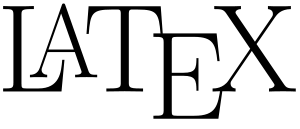
\includegraphics[width=4cm]{logo}}
%  
%% If you are not creating a PDF then use the following. The default is PDF.
%\else
%  \author{YourName}
%%  \cityofbirth{born in XYZ}
%  \collegeordept{CollegeOrDept}
%  \university{University}
%  \crest{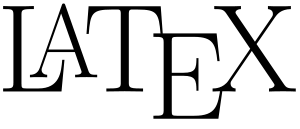
\includegraphics[width=4cm]{logo}}
%\fi

\ifpdf
%  \author{\href{mailto:hami0003@ntu.edu.sg}{Hamid Reza Sharifzadeh}}
  \author{{Thanh-Hai Le}}
%  \cityofbirth{born in XYZ} % uncomment this if your university requires this
%  % If city of birth is required, also uncomment 2 sections in PhDthesisPSnPDF
%  % Just search for the "city" and you'll find them.
%  \collegeordept{\href{http://www.something.net}{CollegeOrDepartment}}
  \collegeordept{{School of Computer Engineering}}
%  \university{\href{http://www.something.net}{University}}
  \university{{Nanyang Technological University}}
 
  % The crest is a graphics file of the logo of your research institution.
  % Place it in ./0_frontmatter/figures and specify the width
  \crest{
\includegraphics[height=2.6cm,width=6.5cm]{Picture1}}
% 
%% If you are not creating a PDF then use the following. The default is PDF.
\else
  \author{{Thanh-Hai Le}}
%%  \cityofbirth{born in XYZ}
  \collegeordept{{School of Computer Engineering}}
  \university{{Nanyang Technological University}}
  \crest{
\includegraphics[height=2.6cm,width=6.5cm]{Picture1}}
\fi

%\renewcommand{\submittedtext}{change the default text here if needed}
\degree{Doctor of Philosophy (PhD)}
\degreedate{Feb 2013}

% ----------------------------------------------------------------------
       
% turn of those nasty overfull and underfull hboxes
\hbadness=10000
\hfuzz=50pt

%: --------------------------------------------------------------
%:                  FRONT MATTER: dedications, abstract,..
% --------------------------------------------------------------
\makenomenclature

\begin{document}

%\language{english}

% sets line spacing
\renewcommand\baselinestretch{1.2}
\baselineskip=18pt plus1pt


%: ----------------------- generate cover page ------------------------

\maketitle  % command to print the title page with above variables


%: ----------------------- cover page back side ------------------------
% Your research institution may require reviewer names, etc.
% This cover back side is required by Dresden Med Fac; uncomment if needed.

%\newpage
%\vspace{10mm}
%1. Reviewer: Name
%
%\vspace{10mm}
%2. Reviewer: 
%
%\vspace{20mm}
%Day of the defense:
%
%\vspace{20mm}
%\hspace{70mm}Signature from head of PhD committee:



%: ----------------------- abstract ------------------------

% Your institution may have specific regulations if you need an abstract and where it is to be placed in the document. The default here is just after title.


% Thesis Abstract -----------------------------------------------------


%\begin{abstractslong}    %uncommenting this line, gives a different abstract heading
\begin{abstracts}        %this creates the heading for the abstract page

In the past decades, the exponential growth in computational power has made the once overly-excessive computationaly-demanding SAR technology now become a feasible and preferred earth observation solution.
As state-of-the-art technology, the SAR technique has been extended in a few directions, one of which is the polarimetric SAR or POLSAR.
POLSAR is the natural extension from SAR exploiting the natural polarization property of Electro-Magnetic (EM) waves.
Similar to the extension from black-and-white images to color photography, the polarimetric extension brought about the multi-channels POLSAR data as compared to the traditional one-channel SAR data.

With (POL)SAR data becomes cheaper and more available, the recent research emphasis is on understanding and developing applications for the data. %it is of great important to understand the data.
The SAR data, however is stochastic by nature, due to the interference phenomena of EM waves. %, SAR measurements are stochastic by nature.
Under this condition, it is very important to understand the statistical models for SAR data.
It is these models that form the foundation for different SAR data processing techniques,
  for example speckle filtering, target detection, image segmentation, and other clustering, classification techniques.
Central to these machine learning or signal processing algorithms is the need for consistent discrimination measures which are derived from the statistical models.

While the statistical models for homogeneous SAR areas have long been developed and widely used,
  in extending the model toward heterogeneous images, the impact of the heteroskedastic property in these models has virtually been ignored.
Specifically the concept of distance as a measure of dis-similarity is seriously flawed,
  as it is widely known that ratio offers a better discrimination measure for SAR \cite{Rignot_1993_TGRS_896}.
This thesis starts off by proposing the logarithmic transformation which is shown converting the SAR data into an homoskedastic model.
Within this log-transformed domain, a few consistent measures of distance is proposed. 
In a sense the distance concept is re-emerged, as the log-transformation converts the widely used ratio into standard subtractive distance.

In extending our statistical understanding of SAR data towards multi-dimensional POLSAR data, an important issue needs to be addressed.
The trouble that the high dimensional data bring about is that there exists not one, as the intensity in the one-channel SAR, but many observables quantities in multi-channel POLSAR.
While different statistical models have been developed for different POLSAR observables,
  for a statistical model to be useful, scalar discrimination measures need to be derived from.
Thus on the one hand, practical application for POLSAR data processing requires the measure to be scalar, consistent and preferably homoskedastic. % on the one hand.
On the other hand, the observable quantity being modelled needs to be naturally representative for the high dimensional POLSAR data.

In this thesis, the determinant of the POLSAR covariance matrix is proposed as an observable quantity to study.
The representative power of this observable is demonstrated when the multi-dimensional POLSAR data is collapsed into the traditional one-dimensional SAR scenario, the determinant then is transformed into the standard SAR intensity.
Statistical models for this heteroskedastic POLSAR determinant and homoskedastic log-determinant are then derived.
And since POLSAR can be viewed as a multi-dimensional extension of SAR, the thesis describes how the standard statistical models for SAR can be put within the natural coverage of this generic models for POLSAR.
%Subsequently logarithmic transformation is investigated for this generalized SAR model,
%  which lead to the proposal for several linear and additive measures of distance for POLSAR.

%There are a few benefits of using the homoskedastic measures of distance for POLSAR.
In short, to address the dual-problem described above,
  this thesis proposes several scalar, additive and homoskedastic measures of distance for the multi-dimensional, multiplicative and heteroskedastic POLSAR data. 
%The proposed statistical models and the homoskedastic measures of distance for POLSAR bring about a couple of benefits. 
There are a couple of benefits in using these homoskedastic measures of distance for (POL)SAR.
First, compared to the multiplicative dis-similarity measure of ratio, these additive measures of distance fit more naturally with the linear nature of digital imagery.
Second, within the homoskedastic log-transformed domain, where the distance concept as well as the Gauss-Markov theorem is again applicable,
  the use of Mean Squared Error (MSE) as universal objective function deserves to be reviewed. % as a reliable objective function / criteria for (POL)SAR estimators.
%This may open up a number of different research directions for future studies of (POL)SAR.
As example applications of how these statistical models and distance measures,
  a novel clustering algorithm, a new speckle filter and various procedures in using MSE to evaluate speckle filters are also presented as part of the thesis.

\end{abstracts}
%\end{abstractlongs}


% ---------------------------------------------------------------------- 

%\pagenumbering{arabic}

% The original template provides and abstractseparate environment, if your institution requires them to be separate. I think it's easier to print the abstract from the complete thesis by restricting printing to the relevant page.
% \begin{abstractseparate}
%   
% Thesis Abstract -----------------------------------------------------


%\begin{abstractslong}    %uncommenting this line, gives a different abstract heading
\begin{abstracts}        %this creates the heading for the abstract page

In the past decades, the exponential growth in computational power has made the once overly-excessive computationaly-demanding SAR technology now become a feasible and preferred earth observation solution.
As state-of-the-art technology, the SAR technique has been extended in a few directions, one of which is the polarimetric SAR or POLSAR.
POLSAR is the natural extension from SAR exploiting the natural polarization property of Electro-Magnetic (EM) waves.
Similar to the extension from black-and-white images to color photography, the polarimetric extension brought about the multi-channels POLSAR data as compared to the traditional one-channel SAR data.

With (POL)SAR data becomes cheaper and more available, the recent research emphasis is on understanding and developing applications for the data. %it is of great important to understand the data.
The SAR data, however is stochastic by nature, due to the interference phenomena of EM waves. %, SAR measurements are stochastic by nature.
Under this condition, it is very important to understand the statistical models for SAR data.
It is these models that form the foundation for different SAR data processing techniques,
  for example speckle filtering, target detection, image segmentation, and other clustering, classification techniques.
Central to these machine learning or signal processing algorithms is the need for consistent discrimination measures which are derived from the statistical models.

While the statistical models for homogeneous SAR areas have long been developed and widely used,
  in extending the model toward heterogeneous images, the impact of the heteroskedastic property in these models has virtually been ignored.
Specifically the concept of distance as a measure of dis-similarity is seriously flawed,
  as it is widely known that ratio offers a better discrimination measure for SAR \cite{Rignot_1993_TGRS_896}.
This thesis starts off by proposing the logarithmic transformation which is shown converting the SAR data into an homoskedastic model.
Within this log-transformed domain, a few consistent measures of distance is proposed. 
In a sense the distance concept is re-emerged, as the log-transformation converts the widely used ratio into standard subtractive distance.

In extending our statistical understanding of SAR data towards multi-dimensional POLSAR data, an important issue needs to be addressed.
The trouble that the high dimensional data bring about is that there exists not one, as the intensity in the one-channel SAR, but many observables quantities in multi-channel POLSAR.
While different statistical models have been developed for different POLSAR observables,
  for a statistical model to be useful, scalar discrimination measures need to be derived from.
Thus on the one hand, practical application for POLSAR data processing requires the measure to be scalar, consistent and preferably homoskedastic. % on the one hand.
On the other hand, the observable quantity being modelled needs to be naturally representative for the high dimensional POLSAR data.

In this thesis, the determinant of the POLSAR covariance matrix is proposed as an observable quantity to study.
The representative power of this observable is demonstrated when the multi-dimensional POLSAR data is collapsed into the traditional one-dimensional SAR scenario, the determinant then is transformed into the standard SAR intensity.
Statistical models for this heteroskedastic POLSAR determinant and homoskedastic log-determinant are then derived.
And since POLSAR can be viewed as a multi-dimensional extension of SAR, the thesis describes how the standard statistical models for SAR can be put within the natural coverage of this generic models for POLSAR.
%Subsequently logarithmic transformation is investigated for this generalized SAR model,
%  which lead to the proposal for several linear and additive measures of distance for POLSAR.

%There are a few benefits of using the homoskedastic measures of distance for POLSAR.
In short, to address the dual-problem described above,
  this thesis proposes several scalar, additive and homoskedastic measures of distance for the multi-dimensional, multiplicative and heteroskedastic POLSAR data. 
%The proposed statistical models and the homoskedastic measures of distance for POLSAR bring about a couple of benefits. 
There are a couple of benefits in using these homoskedastic measures of distance for (POL)SAR.
First, compared to the multiplicative dis-similarity measure of ratio, these additive measures of distance fit more naturally with the linear nature of digital imagery.
Second, within the homoskedastic log-transformed domain, where the distance concept as well as the Gauss-Markov theorem is again applicable,
  the use of Mean Squared Error (MSE) as universal objective function deserves to be reviewed. % as a reliable objective function / criteria for (POL)SAR estimators.
%This may open up a number of different research directions for future studies of (POL)SAR.
As example applications of how these statistical models and distance measures,
  a novel clustering algorithm, a new speckle filter and various procedures in using MSE to evaluate speckle filters are also presented as part of the thesis.

\end{abstracts}
%\end{abstractlongs}


% ---------------------------------------------------------------------- 

% \end{abstractseparate}


%: ----------------------- tie in front matter ------------------------

\frontmatter
% Thesis Dedictation ---------------------------------------------------

\begin{dedication} %this creates the heading for the dedication page

To those in need, 

With love and hard work.
%from the love for humanity!!!

\end{dedication}

% ----------------------------------------------------------------------

% Thesis Acknowledgements ------------------------------------------------


%\begin{acknowledgementslong} %uncommenting this line, gives a different acknowledgements heading
%\begin{acknowledgements}      %this creates the heading for the acknowlegments

\section*{Acknowledgement} %this results in an overhead bar,  
\pagestyle{empty} %this removes the bar
%\addcontentsline{toc}{chapter}{Acknowledgement}

\epigraph{\textit{``Not many appreciate the ultimate power and potential usefulness of basic knowledge accumulated by obscure, unseen investigators who, in a lifetime of intensive study, may never see any practical use for their findings but who go on seeking answers to the unknown without thought of financial or practical gain.''}}%
{\textit{}\\ \textsc{Eugenie Clark}}

\onehalfspacing

Before anything, I would like to express my gratitude towards my family, specifically my wife, my parents and my kids,
  whose constant love and unconditional support I have greatly relied upon. 
Their immeasurable sacrifices together with their continous encouragement have always been the motivation for me to follow this academic pursuit.
%venture further. 
%It is ultimately to them that this work is dedicated.
They are the first and foremost people that this work is dedicated upon.

This thesis would also not have been possible without the patient and helpful guidance of Assoc. Prof. Ian McLoughlin and Assoc Prof. Nicholas Vun Chan Hua, 
	under whose supervision I am gratefully being under. 
The supervisors have been providing firm support, as well as spot-on guidance. 
During all the stages of my research work, 
	be it conceptualization or result analysis, be it writing, presentation or publishing ..
	their kind attention and wise advices command my utmost respect and admiration.

%The author also wish to thank Dr. Timo Brestchneider and Dr. Lee Ken Yoong, whose suggestions and knowledgable feedbacks have always been greatly appreciated. 
%Their continued efforts, together with EADS's various other contributions have greatly enhanced the quality of this research. 

Special thanks go to my friends and colleagues, whose friendship and companion have made the journey a truly enjoyable one. 
They include but not limited to: Brian Nguyen Quang Huy, Erwin Anggadjaja and Hamid Reza Sharifzadeh ...

Last but not least I would like to give my appreciations to all NTU staffs at PDCC, SCE and GSO whose quiet but continous supporting efforts played a very important role in any measure of success this dissertation may be associated with.

\begin{flushright}
	\parbox[t]{1\textwidth}{%b
	\begin{flushright}
		\emph{{}``The roots of education are bitter, but the fruit is sweet.''}\\
		\emph{--} Aristotle\\
	\par\end{flushright}%
	}	
\par\end{flushright}

%\end{acknowledgements}
%\end{acknowledgmentslong}

% ------------------------------------------------------------------------



\pagenumbering{roman}

%: ----------------------- contents ------------------------

%\addcontentsline{toc}{chapter}{Table of Contents}
\setcounter{secnumdepth}{3} % organisational level that receives a numbers
\setcounter{tocdepth}{3}    % print table of contents for level 3

\phantomsection
\addcontentsline{toc}{chapter}{Content Tables}
\tableofcontents            % print the table of contents
% levels are: 0 - chapter, 1 - section, 2 - subsection, 3 - subsection

%: ----------------------- glossary ------------------------

% Tie in external source file for definitions: /0_frontmatter/glossary.tex
% Glossary entries can also be defined in the main text. See glossary.tex
%% this file is called up by thesis.tex
% content in this file will be fed into the main document

% Glossary entries are defined with the command \nomenclature{1}{2}
% 1 = Entry name, e.g. abbreviation; 2 = Explanation
% You can place all explanations in this separate file or declare them in the middle of the text. Either way they will be collected in the glossary.

% required to print nomenclature name to page header
\markboth{\MakeUppercase{\nomname}}{\MakeUppercase{\nomname}}


% ----------------------- contents from here ------------------------

\nomenclature{SAR}{Synthetic Aperture Radar} 
% chemicals
\nomenclature{DAPI}{4',6-diamidino-2-phenylindole; a fluorescent stain that binds strongly to DNA and serves to marks the nucleus in fluorescence microscopy} 
\nomenclature{DEPC}{diethyl-pyro-carbonate; used to remove RNA-degrading enzymes (RNAases) from water and laboratory utensils}
\nomenclature{DMSO}{dimethyl sulfoxide; organic solvent, readily passes through skin, cryoprotectant in cell culture}
\nomenclature{EDTA}{Ethylene-diamine-tetraacetic acid; a chelating (two-pronged) molecule used to sequester most divalent (or trivalent) metal ions, such as calcium (Ca$^{2+}$) and magnesium (Mg$^{2+}$), copper (Cu$^{2+}$), or iron (Fe$^{2+}$ / Fe$^{3+}$)}



 
%
%\begin{multicols}{2}  %\begin{multicols}{#columns}[header text][space]
%\begin{footnotesize}  %scriptsize(7) < footnotesize(8) < small (9) < normal (10)
%
%\printnomenclature[1.5cm]  %[] = distance between entry and description
%\label{nom}  %target name for links to glossary
%
%\end{footnotesize}
%\end{multicols}

\chapter*{List of Symbols}
\addcontentsline{toc}{section}{List of Symbols}

\section*{1. Glossary}

\begin{multicols}{2}
  
%Glossary: includes term: definition

%Acronym: includes acronym: full term; definition?

{\bf Polarimetric Synthetic Aperture Radar:} the extension of single-channel SAR imaging solution to multiple-channel imagary using polarimetric properties.\\

{\bf POLSAR:} Polarimetric Synthetic Aperture Radar \\

{\bf SAR:} Synthetic Aperture Radar\\

{\bf Synthetic Aperture Radar:} an active side-looking-radar remote sensing solution based on doppler-effect\\

\label{glossary} % target name for links to glossary

\end{multicols}

\newpage

\section*{2. Nomenclatures}

\begin{multicols}{2} % \begin{multicols}{#columns}[header text][space]  produces a 2 column page for a compact glossary
%\begin{footnotesize} % scriptsize(7) < footnotesize(8) < small (9) < normal (10)

$C_v$: denotes the {\bf polarimetric covariance matrix}\\

$C_h$: denotes the {\bf polarimetric coherency matrix}\\

$M^{*T}$: denotes the {\bf complex conjugate transpose} of matrix $M$ \\

$pdf(x;k)$: denotes the {\bf probability density function} of the {\bf random variable} $x$,
  given the known and {\bf constant} $k$\\

$cdf(x;k)$: denotes the {\bf cumulative distribution function} of the {\bf random variable} $x$,
  given the known and {\bf constant} $k$\\  

$cf(x;k)$: denotes the {\bf characteristic function} of the {\bf random variable} $x$,
  given the known and {\bf constant} $k$\\  

$X \sim Y$: denotes the observable values $X$,
  which behaves as a single or a combination of random process(es) $Y$. 
  
$|M|$: denotes the {\bf determinant} of the matrix $M$, also denoted as $det|M|$\\

$Z$: denotes the {\bf scaled polarimetric covariance matrix}, $Z=LC_v$ (see: $C_v$)\\

$\Gamma(x)$: denotes the {\bf Gamma function}.\\

$tr(M)$: denotes the {\bf trace} of matrix $M$.\\

$\chi^2(2L)$: denotes the {\bf Chi-Square distribution} with $2L$ degrees of freedom.\\

$\Lambda(2L)$: denotes the {\bf Log-Chi-Square distribution} with $2L$ degrees of freedom.\\
  
  
%\end{footnotesize}
\end{multicols}

%: ----------------------- list of figures/tables ------------------------

%\pagenumbering{roman}
\newpage
\listofmyequations
\addcontentsline{toc}{section}{List of Equations}
%\phantomsection
%\addtocontents{toc}{List of Equations}

\newpage
\renewcommand\lstlistlistingname{List of Source Code}
%\renewcommand\lstlistingname{Algorithm}
\lstlistoflistings
\addcontentsline{toc}{section}{List of Source Code}

\newpage
\listoffigures	% print list of figures
\addcontentsline{toc}{section}{List of Figures}

\newpage
\listoftables  % print list of tables
\addcontentsline{toc}{section}{List of Tables}

%\chapter*{List of Mathematic Symbols}
%\addcontentsline{toc}{section}{List of Mathematic Symbols}
%
%\begin{multicols}{2} % \begin{multicols}{#columns}[header text][space]  produces a 2 column page for a compact glossary
%\begin{footnotesize} % scriptsize(7) < footnotesize(8) < small (9) < normal (10)
%
%%Nomenclature: includes math term: definition
%
%$C_v$: Polarimetric Covariance Matrix\\
%
%$C_h$: Polarimetric Coherence Matrix\\
%
%\label{nom2} % target name for links to glossary
%
%\end{footnotesize}
%\end{multicols}

%: --------------------------------------------------------------
%:                  MAIN DOCUMENT SECTION
% --------------------------------------------------------------

% the main text starts here with the introduction, 1st chapter,...
\mainmatter
\pagestyle{plain}
\pagenumbering{arabic}

%\renewcommand{\chaptername}{} % uncomment to print only "1" not "Chapter 1"


%: ----------------------- subdocuments ------------------------

% Parts of the thesis are included below. Rename the files as required.
% But take care that the paths match. You can also change the order of appearance by moving the include commands.

%: ----------------------- introduction file header -----------------------
\chapter{Introduction}

%What is the situation, the background context of your research? the BIG problem!
Synthetic Aperture Radar is a technology with many advantages.
%Compared to optical remote sensors, which are passive, active SAR sensors provide weather independent and night-inclusive operational capabilities.
Compared to optical remote sensors - which are passive, SAR uses active sensors to provide weather independent and night-inclusive operational capabilities. 
Compared to other radar based active sensors,
for example Real Aperture Radar (RAR), SAR provides state-of-the-art resolution
and coverage.
In the past decades, the exponential growth in computational power has made the once overly excessive computationally demanding SAR technology to become a feasible and preferred earth observation solution \cite{Cumming_2005_Artech}.
Thus SAR has now become the preferred choice for continuous and autonomous large-scale
remote surveillance solutions.

As state-of-the-art technology, the SAR technique has been extended in a few directions, one of which is polarimetric SAR or POLSAR. POLSAR is the natural
extension from SAR, exploiting the natural polarization property of Electromagnetic
(EM) waves. It extends the SAR acquisition information from the traditional single
SAR channel to multi-channel polarimetric SAR data, corresponding to a different combination of transmitted and received polarizations. Similar to the extension from black-and-white images to colour photography, the polarimetric extension brought about
multi-channel POLSAR data as compared to the traditional one-channel SAR data.

With both SAR and POLSAR data becoming cheaper and more available, the recent research emphasis is on understanding and developing applications for the data. However, both SAR 
and POLSAR suffer from speckle phenomena, which hampers the human capabilities
to understand SAR images. Speckle arises due to the random interference of many
de-phased but coherent backscattered waves. Thus both SAR and POLSAR data are
stochastic by nature.

\section{Research Motivation}

%Given the BIG problem, Why it is important to solve this problem?
The
                big picture, as introduced above, is that POLSAR data is multi­dimensional,
                stochastic, multiplicative and heteroskedastic.
%Under
%                this context, the motivation is to gain a better
%                understanding of the data,
%which
%                hopefully will lead to better information that can be
%                extracted from these data.
Under this condition, it is very important to understand the statistical models for SAR
data. It is these models that form the foundation for different SAR data processing
techniques, for example speckle filtering, target detection, image segmentation, and
other clustering, classification techniques.
In fact, due to the random nature of speckle, all of these techniques are essentially based on statistical estimation theory,
which comprises statistical modeling and validation, estimator design and development
as well as evaluation of different estimators’ accuracy. And central to this statistical
estimation theory is the need for statistically consistent discrimination measures which
are commonly derived from the statistical models.

That is, while different statistical models have been developed for different POLSAR
observables, for a statistical model to be useful, scalar discrimination measures need to
be derived from it. At the same time, the extension from SAR to POLSAR brings about
a representation difficulty in that: there exists not one, like the intensity in SAR, but
many observable quantities in POLSAR. Thus on the one hand, practical application for
POLSAR data processing requires the measure to be scalar, consistent and preferably
homoskedastic. On the other hand, the observable quantity being modeled needs to
be naturally representative of the high dimensional POLSAR data.

%Solving these dual-problem is both important and interesting.
%The statistical models are undoubtedly important in understanding the stochastic nature of the data. 
%At the same time, the statistical properties of the input data set greatly affect the choice and the performance of information extraction and statistical estimation techniques.
In addition, most of these data processing techniques are traditionally designed for additive and homoskedastic data.
In fact, unless proven otherwise, it is both convenient and acceptable to assume that the additive white noise model is appropriate for any given set of data samples.
This is due to a number of reasons, for example the prevalence of the normal distribution which results from the central limit theorem, or the prevalence of the additive noise model which probably arises due to the linear and additive nature of digital data. % dear Ian I changed this back 
%of the Additive White Gaussian Noise (AWGN) model in natural processes.
%of the additive noise model which probably arises due to the linear and additive nature of digital data.%****IVM I'm not sure about this - you seem to assume (in this sentence) that digital data is linear and additive. However this is definitely not true - your POLSAR data is digital and yet is not additive. Maybe you can say "or the prevalence of AWGN in the majority of sensing or sampling systems, and electronic devices."
%OR PERHAPS THIS: "... the prevalence of AWGN in natural processes."
It should be noted that even for the case of SAR data which is digital and not additive,
  the above statement is still true as SAR actually has two components, real and imaginary part,
  and all of them follows the standard Additive White Gaussian Noise model.

Both SAR and POLSAR data however is multiplicative and heteroskedastic by nature.
While there is no doubt that a number of data processing techniques have been proposed to handle certain aspects of the data, the breadth and depth of these studies trails in comparison to that of the more familiar additive and homoskedastic model.
This leads to the fact that a lot of times, existing statistical or computational techniques initially designed for additive and homoskedastic models are applied on multiplicative and heteroskedastic data, in ignorance of the incompatibility. 
An example is the use of mean, variance and squared error criteria, which are linear by nature and works excellently on additive and homoskedastic models, being applied on multiplicative and heteroskedastic distribution such as the gamma distribution.
Such use, however, is known to be not very robust for these so-called heavy tailed distributions.

Similarly speaking, heteroskedasticity poses numerous negative impacts on the usual framework of statistical estimation, which most of the time makes use of various different techniques and criteria known to work very well on the usual models.
For example, in modelling, it is very common to use subtractive differences to discriminate and to make decisional inferences. However for heteroskedastic SAR, it is known that such use should be avoided in preference to a ratio-based discrimination measure.
Another example is in the normal performance evaluation stage of statistical estimators, where the Ordinary Least Square (OLS) is widely used as the best evaluation criteria which is probably due to the Gauss Markov theorem.
For SAR data, however, its heteroskedasticity directly violates the homoskedastic assumption of the theorem and thus many different ways to evaluate SAR speckle filters were proposed.

Furthermore, since POLSAR can be considered as the multi-dimensional extension of
traditional SAR, a common problem exists for both SAR and POLSAR data. That
is: the sense of subtractive distance is seriously flawed in the original multiplicative
and heteroskedastic domain of both types of data. 
In contrast, the digital technologies which range from image processing and display to artificial intelligence and machine learning algorithms used to process (POL)SAR data are linear
and additive in nature. 
This linear and additive nature is manifested, for example, in a
large number of algorithms in the field of computational intelligence which make use of
MSE as an objective function, as well as the extensive use of variance and
contrast in digital image processing. 
Thus it is very exciting to derive homoskedastic models for this heteroskedastic data
  so that the benefits of an additive and homoskedastic statistical estimation framework can be explored.

%Specifically, 
%  this thesis focuses on providing a solution for the
%                dual-problem of: 1) developing scalar and
%                representative statistical models for the
%                multi-dimensional and inter-correlated POLSAR data and
%                2) establishing at consistent measures of distance for both
%                SAR and POLSAR data which allow the benefits of the
%                homoskedastic statistical estimation framework to be
%                demonstrated.


\section{Research Objective}

%The research objectives 
%helps to 1) define and focus your effort, 2) identify variables to be measured 3) identify steps to be performed 4) establish the limits of the study 5) avoid any data collection, argument development that is not necessarily needed.
%Should be stated in action verbs specific enough to be measurable. Avoid vague, non-active verbs which is hard to evaluate if the objectives have been achieved.
%4. Research methodologies (How the research is/was/will be conducted)
%5. Result interpretation and evaluation (describe how the results is expected to look like, how they are going to be evaluated

%How do others solve this problem?
%Briefly What are their solution? what problems they cannot yet solve?
While
                the statistical model for SAR is quite well understood,
the
                understanding of the POLSAR statistical model trails behind.
The
                complex POLSAR data have been statistically modelled as
                following the complex Wishart distribution, which
                apparently is multi­dimensional, complex and
                un­intuitive.
There
                has been a few published scalar statistical models for
                POLSAR, but none of them fit the dual criteria of being
                highly representative of the data and at the same time
                lead to scalar discrimination measures.
There
                are also a few POLSAR discrimination measures proposed,
                but all of them are based on the likelihood test
                statistics, which so far have only shown to be based on an
                asymptotic distribution.

 In
                another thread of study, to combat the negative
                impacts caused by multiplicative and heteroskedastic
                properties for SAR data, experienced researchers of the
                field have developed numerous ingenious ways to tackle
                these issues.
For
                example, when the sense of subtractive distance is not
                consistent for SAR data, the ratio is proposed as its
                discrimination measure \cite{Rignot_1993_TGRS_896}.
Or
                when the MMSE criteria is not very suitable to evaluate
                SAR speckle filters, other criteria likes radiometric
                preservation and speckle suppression power evaluation
                are employed. 
Unfortunately,
                these counter­intuitive measures are not very popular
                outside the SAR community, and newcomers to the field
                are frequently found being trapped in these pitfalls.

%In what way is your solution different ? What is the novelty in your approach and hence solution?
Some of the problems described above have been studied using different approaches in the literature.
However, the set of problems has not been presented in a systematic manner nor with a strong underlying foundational theory.
In
                this thesis, the statistical model for the determinant
                of the POLSAR covariance matrix is proposed and
                validated.
Out
                of many different possible scalar projections of the
                multi-dimensional data, the proposed projection is
                highly representative.
When the dimension number is collapsed to one, the
                special case of the proposed model matches perfectly
                with the commonly used statistical model for SAR
                intensity.
Furthermore,
                the proposed statistical model also leads to the
                derivation of existing as well as the newly proposed
                discrimination measure: determinant-ratio which is the
                generalized multi dimensional version of the widely used
                SAR intensity ratio.

 Another
                novelty of the contributions in this thesis comes from the systematic
                treatment towards the problem of statistical estimation
                of heteroskedastic SAR data.
While
                many different ways to combat the negative impacts
                caused by multiplicative and heteroskedastic properties
                for SAR data have been proposed over the years, they have often been
                handled in a piecemeal manner.
Here,
                a systematic homoskedastic framework of statistical
                estimation is developed, where not only homoskedastic
                statistical models are proposed, the impacts of
                homoskedasticity on estimator development and
                performance evaluation of statistical estimators is also
                studied.
This
                comprehensive treatment not only explains why the
                original SAR data requires special treatment very
                different to the common practice of computational
                sciences, 
it
                also allows thorough and unique discussion, for example on
                evaluating different evaluation criteria for statistical
                estimators.  % ;-)).
And
                since the POLSAR data can be considered as the multi
                dimensional extension of traditional SAR data, these
                treatments are shown extensible towards POLSAR data
                which is definitely yet another novelty. 

%precise problem statement
With this approach, the \textbf{main problem statement} of this thesis arise. %it is important to emphasize again the main problem statement of this thesis.
That is
                this thesis focuses on providing a solution for the
                dual-problem of: 1) establishing scalar and
                representative statistical models for the
                multi-dimensional and inter-correlated POLSAR data and
                2) providing consistent measures of distance for both
                SAR and POLSAR data which allow the benefits of the
                homoskedastic statistical estimation framework to be
                demonstrated.

\section{Research Methodology}
%To achieve the stated objectives, what is your plan of attack? Describe How your actions are to be conducted? How your argument is developed?                
%****IVM Hai, I removed this sentence. I don't think it adds anything useful...
%The bottom up development of the research effort for this long-term study, admittedly is not as straightforward as the top down layout of the stated objectives.
The
                overall research methodology is to first focus on the
                simpler one dimensional SAR domain, and then extend the
                obtained insights and processing techniques 
towards the more complex multi dimensional
                POLSAR data domain.
%***IVM   what OPEN LOOP??? I'm not sure that this is an open loop!! Can't you just say "This is achieved when....."
This
                is achieved as the theoretical models for
                POLSAR are shown to be the multi dimensional extensions of
                the one dimensional SAR model.

The
                development of these models are based on
                rigorous statistical mathematics transformations. % and theory. 
The
                assumptions used are minimal and widely
                acknowledged for this type of data.
Then, the variable change theorem is applied to derive the statistical model for these transformed observables. %log-transformed SAR data.
The
                derived theoretical models are validated against
                real life data.
And
                the imperfect conditions found in practice (in
                comparison to the theoretical assumption) are also
                investigated, and the models are shown to be robust, capable of
                handling these imperfections.
The
                theoretical properties of these models, as well as many
                of their benefits, are also proven using rigorous
                mathematical principles.

%The theoretical statistical models are derived from the commonly used statistical models for SAR and POLSAR.
%Then, as mentioned above, the variable change theorem is applied to derive the statistical model for log-transformed SAR data.
%A similar methodology is then followed for the multi-dimensional POLSAR data.
%The POLSAR theoretical foundation used is the Complex Wishart distribution applicable on the covariance matrix.
%In this thesis, the statistical model for the determinant of this covariance matrix,
%  is derived from this foundation.
%The variable change theorem is again applied to derive the discrimination measures from these derived basic models.
  
As both the SAR and POLSAR data are stochastic in nature, many of the associated data processing techniques, such as speckle filtering has been put into the framework of statistical estimation.
For such application, the research methodology is based extensively on the statistical estimation framework. 
The framework consists of three stages:

%***IVM Hai, I changed your list type to make it look better
\begin{description}
\item{Stage 1:} data statistical analysis. 
We propose a preferred data transformation and decomposition that may allow applications of existing computer science techniques. 
The statistical models built after such a transformation are validated against real-life data.
\item{Stage 2:} predictor and estimator development.
Various statistics-based computational intelligence and/or signal processing methods are to be applied. 
\item{Stage 3:} results analysis and performance evaluation.
Experiment results are evaluated both qualitatively on real images and quantitatively through simulated data. 
\end{description}

\subsection{Statistical Estimation Framework for (POL)SAR data}

Even though the research topic seems to spread across different sub-fields, the common framework that binds them all together is the application and development of statistical estimators.
For speckle filtering, it is the estimation of underlying back-scattering coefficients being corrupted with stochastic noise.
For the problem of target detection or classification,
  it is the estimation of the likelihood that the target belongs to a certain category.

Thus a significant portion of this research effort focuses on developing a computational framework for simulation, evaluation, processing and classification of target polarimetric signatures.
The benefits of such a framework are many fold.
Firstly, simulation allows one to quickly carry out experiments on small synthesized and well-designed scenarios, without the need for highly expensive satellite imagery.
Secondly, simulation provides ground-truth, without which quantitative evaluation of estimators would have been impossible.
Last but certainly not least, such a framework allow one to apply estimators repeatedly, and results from different estimators can be statistically and reliably compared. For example, allowing different authors to compare results quantitatively.

The objective of such framework being:
\begin{enumerate}
\item To build, develop and validate statistical models for different stochastic processes that are inherent within the polarimetric SAR domain.
\item To allow easy, fast and repeatable simulations and experiments of various stochastic processes in designed, focused, as well as broad-based scenarios.
\item To allow easy application of different existing estimators as well as various transformations into focused and simulated scenarios as well as into practical real measured data.
\item To allow development and calculation of good performance indices for estimators. 
\item To allow visualization and analysis of the performance of different stochastic estimators.
\item Ultimately, to allow development of better and more accurate estimators, whose results can be verified: not only qualitatively on real life images, but also quantitatively through rigorous simulations.
\end{enumerate}

The possible benefits of this computational framework are:
\begin{enumerate}
\item Practical benefits
\begin{enumerate}
\item The computational frameworks allow for faster, quicker and more focused experiments. 
Often, a statistical hypothesis can be observed or rejected by designing and implementing an appropriate computational experiment.
\item The framework allows for easier analysis, and thus more insight to be gained, on the performance of an estimator. 
This, in turn, allows for design and development of better estimators.
\end{enumerate}
\item Academic benefits
\begin{enumerate}
\item The computational framework allows for quantitative evaluation and comparison of estimators.
With fast and repeated experiments, the framework allows one to not only compute a single performance value on a single experiment, but also to analyze the whole behaviour of such performance measures over repeated stochastic simulations.
\item Thus the computational framework provides significant help in deriving new performance evaluation criteria for statistical estimators.
\end{enumerate}
\end{enumerate}

\subsection{Data Collection}

This work has made extensive use of simulated data, which have a number of advantages listed below:
\begin{enumerate}
\item Once the model is validated against real-life data, simulated experiments can be carried out on more focused scenarios.
This allows smaller data sets to be generated and analysis can become faster and more accurate.
\item Contrary to real-life images where underlying coefficients are to be estimated, ground truth is readily available in simulated experiments.
\item Quantitative evaluation is possible not only via a single experiment on a single real-image but via repeated stochastic runs. 
\item Thus not only single values of mean or mean-squared-error are to be evaluated. 
As the whole response PDF is available, statistical bias or heteroskedasticity can also be reported.
\end{enumerate}

Besides simulated  data, we have gathered a large amount of real-life data.
Table \ref{tbl:collected_data} lists data made available to us, courtesy of EADS Innovation Works Singapore. 

\begin{table}
\centering
\begin{tabular}{|c|c|c|}
\hline
Radar Platform & Polarization Mode & Data Capture Time \\
\hline
RadarSat 2 & Full Quad Pol & 29 Apr 2009 \\
RadarSat 2 & Full Quad Pol & 05 Apr 2009 \\
RadarSat 2 & Full Quad Pol & 12 Mar 2009 \\
RadarSat 2 & Full Quad Pol & 23 Jan 2009 \\
RadarSat 2 & Full Quad Pol & 30 Dec 2008 \\
RadarSat 2 & Full Quad Pol & 06 Dec 2008 \\
RadarSat 2 & Full Quad Pol & 19 Oct 2008 \\
RadarSat 2 & Full Quad Pol & 12 Nov 2008 \\
RadarSat 2 & Full Quad Pol & 25 Sep 2008 \\
TerraSar-X & Dual Pol (HH-VV) & 18 Apr 2008 \\
NASA-JPL AirSar & Full Quad Pol & 2001 \\
\hline
\end{tabular}
\caption{Collected imagery data}
\label{tbl:collected_data}
\end{table}

\subsection{Result Interpretation and Evaluation}

%How do you evaluate your solution? 
The
                achievement of the research objectives stated above not only provides
                novel solutions to the stated problem, it also
                illustrates the advantages and beneficial implications
                of the proposed theory.  
Compared
                to existing published techniques, the advantage of the
                proposed theory is qualitative, which does not require
                direct quantitative comparisons.
Instead
                a straightforward binary evaluation would be sufficient.
For
                the POLSAR scalar model, its advantages are that not
                only does it lead to consistent discrimination measures, it
                also generalizes the traditional model for one
                dimensional SAR intensity.
For
                the homoskedastic models, their advantage is that they
                enable an additive and homoskedastic statistical
                framework, which is not only capable of overcome various
                negative impacts of heteroskedasticity, but also results
                in a single better evaluation criteria that can combine
                and represent many different existing performance
                criteria.
                
To validate the theoretical models,  real-life data are used in this work.
Specifically, estimated theoretical PDFs are plotted against the histogram of real data,
  and a good visual match indicates a good validation.
In cases where theoretical PDF cannot be derived, simulated data are then generated
  and their histograms are matched against real-life practical data for validation.

%***IVM This was all said before...
%Simulated experiments allows evaluation of estimators against ground-truth.
%Errors can be quantitatively analyzed and methods to reduce such errors can be developed.
%Thus simulated experiments could produce quick results, which may provide faster analysis and 
%further insights for developing more accurate estimators.

To evaluate the models’ application in statistical estimation framework, a practical point of view is adopted.
Practically, all estimators would eventually need to be applied on and work for real images.
Contrary to experiments on simulated data, experiments on real images often can only be compared qualitatively.
This however is critical and will always be included in our investigations.
The reason is that this helps to guard against any systematic errors in the various assumptions and approximations made in developing the theoretical models.
Towards that end, real-data can help to build and validate statistical models.

\section{Research Contributions}
% How do you know if the problem is solved?   State your research objectives
Interestingly, the dual-problem stated above are found to have a single solution.
They are the derivation of scalar, representative and homoskedastic measures of distance for the POLSAR data
  which is multidimensional, inter-correlated and heteroskedastic

Specifically, the following sub-objectives are to be achieved
\begin{enumerate}
\item                 To derive scalar and representative statistical models
                for the multi-dimensional and inter-correlated POLSAR
                data.
                \begin{enumerate}
                \item \label{itm:polsar_model} To derive a scalar statistical model for the
                POLSAR observable, being the determinant of the
                covariance matrix.
                \item \label{itm:polsar_discrimination_measure} To derive consistent discrimination measures for
                the observable being modeled 
                \item \label{itm:polsar_include_sar} To illustrate its representation power by showing
                that when the multi-channel POLSAR data is collapsed
                into the traditional one-channel SAR data, this
                determinant is transformed into the representative SAR
                intensity.
                \item \label{itm:polsar_validation} To validate the model against practical real-life
                captured POLSAR data.
                \item \label{itm:extend_sar_to_polsar} To demonstrate an example where an existing SAR
                processing technique is extensible towards POLSAR data
                \end{enumerate}
\item                To derive homoskedastic statistical models for the
                heteroskedastic (POL)SAR data. 
                \begin{enumerate}
                \item \label{itm:log_transform} To show that (POL)SAR data are heteroskedastic in
                the original domain and logarithmic transformation
                can convert this into a homoskedastic model.
                \item \label{itm:sar_measures_distance} To derive homoskedastic measures of distance for
                the multi dimensional POLSAR as well as for the one
                dimensional SAR data.
                \item \label{itm:sar_validation} To validate these statistical models against both
                practical SAR and POLSAR data
                \item To illustrate the beneficial applications of these
                statistical models. Specifically:
                \begin{enumerate}
                \item \label{itm:filter_vicious_circle} To show how the consistent sense of variance
                helps break the vicious cycle in the problem of SAR
                speckle filtering: a new statistical test for
                homogeneity and a new speckle filter is derived.
                \item \label{itm:log_mse} To show how the consistent sense of subtractive
                distance helps in the problem of evaluating (POL)SAR
                speckle filters: the log-MSE is proposed to combine the
                evaluation of radiometric preservation and speckle
                suppression power.
                \end{enumerate}
                \end{enumerate}
\end{enumerate}

In summary, the first main objective is to derive a scalar and representative statistical model for POLSAR data.
%The theoretical foundation is the commonly agreed Circular Complex Normal distributions proposed in \cite{Goodman_JOptSocAm_76}. %***IVM you need a reference here!!
%Theory development is based on applying the statistical variable change theorem on the proposed scalar observable.
%The theoretical model is validated by matching the functional PDF or the simulated histogram with real-life captured data.
The second main objective is to derive homoskedastic measures of distance despite its multiplicative and heteroskedastic nature.
This is first applied on the simpler case of SAR data. %devided into a few smaller objectives.
%For this purpose, first log transformation is shown to not only convert the multiplicative noise model into an adaptive one, 
%  it also results in a homoskedastic statistical model.
%From this consistent sense of variance, the second step illustrates the consistent sense of contrast and distance.
%After these models are validated against practical data, their beneficial applications are further explored.
To combine these two seemingly disconnected threads of research, the above results for SAR are extended to POLSAR,
  since the thesis also shows that the POLSAR models are a generic multi-dimensional superset of the traditional SAR data.%***IVM I changed "version" to "superset" in the sentence above. Please check if you are comfortable with that change, and if not, change it back!
Thus the homoskedastic theoretical models and their benefits are extended from SAR to POLSAR.   
%The 3 paragraphs are collapsed into 1: to address Prof Vun's comment:
%(comment: you are stating the objectives repetitively so far – I counted three time so far, and confuse the results obtained with the objectives. There is no need to re-emphasize the objective if the write-up is clear)


\section{Organisation of the Thesis}
The rest of this thesis is organized into five chapters, as follows:
The next chapter will survey the related publications
  and state-of-the-art techniques in modelling, processing, filtering and evaluating (POL)SAR speckle filter will be presented.
It will also discuss the different measures of distance for both SAR and POLSAR data, together with their extensive applications. 
Through these discussion, the need for a homoskedastic and scalar model for the multivariate and heteroskedastic POLSAR is brought forward.

%\section{Research Contributions}

%1 show that the results is not only new but also useful
%2 let the reader read the contribution and says: “gosh, if they can really deliver this, that’s exciting; I’d better read on” 
%new theory or hypotheses, writers will need to explain shortcomings in existing theories.
%new solution, writers will need to explain 1) existing problems and clarify how their solutions solve these problems 2) they also need to compare and contrast a range of alternative solutions and explain why their solution is the best among these alternatives.
%new territory, writers need to make a case for why this new territory is important to study and show that it has been overlooked by previous research.
%new methodology, then writers need to 1) critique the methods of previous studies (or characterize them as inconclusive) and 2) explain how they will address these flaws.

%Show that you deliver on the objectives 
%****IVM   Hai, again I've deleted this sentence because it is slightly negative:
%Even
%                though there are small differences between the bottom up
%                development of the research efforts and the top down
%                stated objectives, the research results of each section
%                contribute to the achievement of the objectives.
%Specifically,
The heart of is thesis contains several contributions which meet the stated objectives.
                Chapter \ref{chap:sar} begins by by highlighting that SAR
                data are heteroskedastic in the original domain, whereas
                logarithmic transformation converts this into a
                homoskedastic model (Research Contribution \ref{itm:log_transform}). 
It
                also drives consistent and homoskedastic measures of
                distance for the one dimensional SAR data (Research Contribution \ref{itm:sar_measures_distance}).
These
                models for SAR are then validated against real-life
                practical data (Research Contribution \ref{itm:sar_validation})

 Chapter
                \ref{chap:polsar} then derives several scalar statistical models for the
                determinant of the POLSAR covariance matrix (Research Contribution \ref{itm:polsar_model}) and
                shows that this is heteroskedastic in the original
                domain as well as homoskedastic in the log-transformed
                domain (Research Contribution \ref{itm:log_transform}).
It
                also derives the heteroskedastic discrimination measures
                (Research Contribution \ref{itm:polsar_discrimination_measure}) as well as several homoskedastic measures of
                distance for the data (Research Contribution \ref{itm:sar_measures_distance}).
Then
                the models for SAR are shown to be a special case of
                the proposed models for POLSAR (Research Contribution \ref{itm:polsar_include_sar}) and finally it
                validates these proposed models (Research Contribution \ref{itm:polsar_validation})

 The
                beneficial applications of these models is presented in
                chapter \ref{chap:applications}, where the consistent sense of variance
                property helps to break the vicious cycle in SAR
                speckle filtering (Research Contribution \ref{itm:filter_vicious_circle}).
It
                also shows how MSE can be again applicable in the
                additive and homoskedastic domain to evaluate SAR
                speckle filters (Research Contribution \ref{itm:log_mse}).
An
                example of extending existing techniques from SAR to
                POLSAR is also demonstrated in this chapter where the
                MSE evaluation criteria is also shown capable of
                evaluating POLSAR speckle filters (Research Contribution \ref{itm:extend_sar_to_polsar}).
Finally, the contribution of the thesis with respect to the research objectives and research impact is discussed in the concluding chapter \ref{chap:conclusions}.


%The heart of the thesis lies in chapters \ref{chap:sar} and \ref{chap:polsar}.
%While chapter \ref{chap:sar} presents the initial homoskedastic model for SAR data, 
%chapter \ref{chap:polsar} illustrates the more recent and more generic model for POLSAR.
%Chapter \ref{chap:polsar} also specifically describes how the initial model for SAR can be considered as a special case of the POLSAR model.
%
%Chapter \ref{chap:applications} presents several of our published techniques in handling both SAR and POLSAR data.
%Theses techniques can all be considered as applications of the theoretical model presented in chapters \ref{chap:sar} and \ref{chap:polsar}.
%Demonstrated applications include clustering algorithms, speckle filtering techniques and a novel methodology to evaluate (POL)SAR speckle filters.

	% background information
%\chapter{Introducing The Research Question}
%STATE: structure stabilized
%TODO: review the content text

%\chapter{Current Methods in Processing SAR and POLSAR Data} %chapter 2
\label{chap:lit_survey}

This chapter 
reviews the published literature for SAR and POLSAR data processing.
Specifically, its first section describes the multi-dimensional and stochastic nature of the POLSAR data.
The second section then illustrates the different approaches that have been published to address the grand challenge of modelling, processing and ultimately understanding these types of data.

\section{The Stochastic and Multivariate Nature of POLSAR data}

\subsection{The Stochastic Nature of SAR data}

%\subsubsection{ Traditional Single-Channel SAR and the Speckle phenomena} 

The stochastic nature of SAR data arises due to the process of SAR image formation. Specifically, since one SAR resolution cell is very big in comparison to the radar wavelength, it normally consists of many elementary scatterers. The data point of each SAR pixel then arises from the combined interference effect of the backscattered waves from these different scatterers. This effect causes natural variation in SAR intensity image even when the underlying scene is highly homogeneous.

SAR speckle phenomena are explained as the interference of many coherent but dephased backscattering components;
  each reflecting from different and distributed elementary scatterers \cite{Oliver_ProcIEEE_1963, Leith_ProcIEEE_1971}. 
The random nature of the SAR data arises
  due to the unknown and varying location, height and thus distance of each elementary scatterer;
  which, in turn, generates random phases in their back-scattering responses.
Assuming the number of these elementary back scatterers is sufficiently large,
  then the Central Limit Theorem is applicable \cite{Goodman_Springer_1975}.
Consequently the interference of these randomly phased responses can be considered as
  a random walk on the 2D complex plane \cite{Goodman_JOptSocAm_76}.  
Specifically the real part $A_r$ as well as the imaginary part $A_i$ of the observed SAR signal $A$ can be considered as
  random variables from uncorrelated Gaussian distributed stochastic processes with zero means and indentical variances $\sigma^2/2$  \cite{Lee_CRCPress_2009}. 
Their probability density functions (PDF) are given as:

\begin{equation}
\label{eqn:SAR Real and Imaginary Components PDF}
\caption{eqn:SAR Real and Imaginary Components PDF}
pdf(A_x)=\frac{1}{\sqrt{\pi} \sigma} e^{\left( \frac{A_x^2}{\sigma^2} \right) }
\end{equation}

It can then be shown that the measurable amplitude $A=\sqrt{A_r^2+A_i^2}$ is a random variable of Rayleigh distribution.
Subsequently the SAR intensity $I=A^2=(A_r^2+A_i^2)$ is a random variable of a negative exponentially distributed random process. The PDFs of these two properties can then be expressed as:

%\begin{eqnarray}
%pdf(A) &=& \frac{2A}{\sigma^2}e^{ \left( -\frac{A^2}{\sigma^2} \right) }\\
%pdf(I) &=& \frac{1}{\sigma^2}e^{\left( -\frac{I}{\sigma^2} \right) }
%\end{eqnarray}
\begin{equation}
\label{eqn:SAR Amplitude PDF}
\caption{eqn:SAR Amplitude PDF}
pdf(A) = \frac{2A}{\sigma^2}e^{ \left( -\frac{A^2}{\sigma^2} \right) }
\end{equation}
\begin{equation}
  \label{eqn:SAR Intensity PDF}
  \caption{eqn:SAR Intensity PDF}
pdf(I) = \frac{1}{\sigma^2}e^{\left( -\frac{I}{\sigma^2} \right) }
\end{equation}

%\subsubsection{The Stochastic nature of SAR  and SAR speckle filtering }

%The stochastic nature SAR arises from the speckle phenomena.
As SAR speckle phenomena arises from the stochastic nature of SAR, it seriously hinders the interpretation and understanding of SAR images.
Speckle noise on SAR images are hence routinely reduced through a speckle filtering process for easier human interpretation and more accurate post-processing.
%***IVM: Hai, I added "human" before 'interpretation'. Also added the text afterwards, please check that the sense of the edited text is still correct in terms of what you wanted to say.

\subsection{The Multivariate Nature of POLSAR data}

\subsubsection{The polarization property of Electro-Magnetic waves}

The propagation of Electro-Magnetic (EM) wave in space is governed by Maxell’s equations. 
The general solution to these equations is a linear superposition of waves, each having the form of:
\begin{eqnarray*}
 \vec{E}(\vec{r},t) &=& g(\phi(\vec{r},t)) = g(\omega t - \vec{k} \cdot \vec{r}) \\
 \vec{B}(\vec{r},t) &=& g(\phi(\vec{r},t)) = g(\omega t - \vec{k} \cdot \vec{r})
\end{eqnarray*}
where
	$g$ is any well-behaved function of a dimensionless argument $\phi$,
	%for virtually any well-behaved function g of dimensionless argument φ, where
	$\omega$ is the angular frequency (in radians per second), and
	$\vec{k}= (k_x,k_y,k_z)$ is the wave vector (in radians per meter).

Because of the divergence between the electric and the magnetic fields, there will be no fields in the direction of wave propagation.
Thus if we define the z direction as the travelling direction of the EM wave,
  then both the electric and the magnetic fields are fluctuating in the x,y plane.
Furthermore, when considering wave propagation, it is conventional that only the electric field vector is described and the magnetic field is ignored since it is perpendicular to the E field and is proportional to it.
Projecting this vector into x,y directions, we have:

\begin{equation*}
\vec{E}(z,t) 
= 
\left(
	\begin{array} {c}
		E_x^0 \cos{ \left( wt - kz  + \phi_x^0 \right) } \\
		E_y^0 \cos{ \left( wt - kz  + \phi_y^0 \right)} \\
		0
	\end{array}
\right)
= 
\left(
	\begin{array} {c}
		\xi_x(t) \\
		\xi_y(t) \\
		0
	\end{array}
\right)
\end{equation*}
where $\phi_0$ is the initial phase angle, that is dependent on the choice of space-time origin.

In other words, the EM vector can oscillate in more than one orientation, and this denote the polarization property of EM wave.
The exact shape traced out in a fixed projective plane by the tip of the electric vector as the plane propagate is a description of the polarization state.
This shape is characterized by the formula: 
\begin{equation*}
 \frac{\xi_x^2(t)}{|E_x^0|^2} + \frac{\xi_y^2(t)}{|E_y^0|^2} - 2 \frac{\xi_x \xi_y}{E_x^0 E_y^0} \cos (\Delta \phi) = \sin^2(\Delta \phi)
\end{equation*}
where
	$\Delta \phi = \phi_y^0 - \phi_x^0$
The formula characterizes what is termed as the polarization ellipse.

The parameters that describe the polarization ellipse are: 
\begin{equation*}
\tan (\theta ) = \frac{E_y^0}{E_x^0}
\end{equation*}
with
	$0 \leq \theta \leq \pi/2$. 
The orientation angle, which is the angle between the major semi-axis of the ellipse and the x-axis, is given by:
\begin{equation*}
\tan (\Psi) = \tan (2 \theta) \cos(\Delta \phi)
\end{equation*}
with
	$0 \leq \Psi < \pi$. 
The ellipticity, $\epsilon$ is the major-to-minor-axis ratio.
The ellipticity angle which is defined as $\chi = \arctan (1/\epsilon)$ can be calculated as:
\begin{equation*}
\sin (2 \chi) = \sin(2 \theta) \sin( \Delta \phi)
\end{equation*}
with
	$0 \leq \chi \leq \pi/2$, and $0 \leq \epsilon \leq \infty$

Ignoring the scale of the electrical fields, the elementary wave polarization can be completely described by two parameters, i.e. $E_y^0/E_x^0$ and $\Delta \phi = \phi_y^0 - \phi_x^0$. 
Similarly, ignoring the scale of the ellipse, the polarization ellipse can be completely described by two angles $\Psi$ and $\chi$.

Other parameters includes:
\paragraph{ Complex polarization ratio }
This ratio is important in explaining polarization basis changes.

It is defined as:
\begin{equation}
\rho = \frac{E_y^0}{E_x^0} e^{i \Delta \phi} = \frac{\cos(2 \chi) + i \sin(2 \chi)}{1 - \cos(2\Psi) \cos(2\chi)}
\end{equation}

\paragraph{Jones Vector}

%Let the total wave power:
%\begin{equation}
%|E|^2 = (E_x^0)^2  + (E_y^0)^2
%\end{equation}
%and phase 
%\begin{equation}
%\theta = \tan^{-1} \left( \frac{E_y^0}{E_x^0} \right)
%\end{equation}

The Jones vector is defined as 
\begin{equation}
J = 
\left(
\begin{array}{c}
	\xi_x(t) \\
	\xi_y(t) 
\end{array}
\right)
= \xi_x(t)
\left(
\begin{array}{c}
	1 \\
	\rho
\end{array}
\right)
\end{equation}

Thus the normalized Jones vector can be given as:
\begin{equation}
J = 
\left(
\begin{array}{c}
	\cos(\theta) \cdot e^{i \phi_x^0} \\
	\sin(\theta) \cdot e^{i \phi_y^0}
\end{array}
\right)
=
\left(
\begin{array}{c}
	1\\
	\tan(\theta) \cdot e^{i \Delta \phi}
\end{array}
\right)
=
\left(
\begin{array}{c}
	\cos(\Psi) \cos(\chi) - i \sin(\Psi) \sin(\chi) \\
	\sin(\Psi) \cos(\chi) + i \cos(\Psi) \sin(\chi)
\end{array}
\right)
\end{equation}

The two parameters in the Jones vector can completely describe the polarization state (ellipse) of any elementary wave.
This same Jones vector finds extensive use in quantum machenics, and is interpreted as quantum state vector.
Its bra-ket notation formula, which is normally used in quantum computation contexts is:
\begin{equation}
J = | \Psi \rangle 
= 
\left(
\begin{array}{c}
	\cos(\theta) \cdot e^{i \phi_x^0} \\
	\sin(\theta) \cdot e^{i \phi_y^0}
\end{array}
\right)
\end{equation}

By definitions, the horizontal linear polarized wave is defined as: $J_h = \left(
\begin{array}{c}
 1 \\
 0
\end{array}
\right)$, similarly the vertical linear polarized wave: $J_v = \left(
\begin{array}{c}
 0 \\
 1
\end{array}
\right)$, the $\pm \pi/4$ linear polarized waves $J_{\pm} = \pm \frac{1}{\sqrt{2}} \left(
\begin{array}{c}
 1 \\
 1
\end{array}
\right)$, the left circular polarized wave: $J_l = |L\rangle = \frac{1}{\sqrt{2}} \left(
\begin{array}{c}
 1 \\
 -i
\end{array}
\right)$ and the right circular polarized wave: $J_r = |R\rangle = \frac{1}{\sqrt{2}} \left(
\begin{array}{c}
 1 \\
 i
\end{array}
\right)$

\paragraph{ Stokes Vector}

Another way to look at polarization is through the coherency matrix, and equivalently the Stokes matrix.
The wave coherency matrix is defined as:
\begin{equation*}
W_c = \left<
\left(
\begin{array}{c}
 \xi_x \\
 \xi_y
\end{array}
\right)
\left(
\begin{array}{c}
 \xi_x \\
 \xi_y
\end{array}
\right)^{\dagger}
\right>
= \left<
\left(
\begin{array}{c c}
 \xi_x \xi_x^* 	& \xi_x \xi_y^* \\
 \xi_y \xi_x^* 	& \xi_y \xi_y^* 
\end{array}
\right)
\right>
= \left<
\left(
\begin{array}{c c}
 |\xi_x|^2 	& |\xi_x| |\xi_y| e^{-i \Delta \phi} \\
 |\xi_x| |\xi_y| e^{i \Delta \phi} 	& |\xi_y|^2
\end{array}
\right)
\right>
\end{equation*}

The Stokes vector is then defined as:
\begin{equation*}
S_t = 
\left(
\begin{array}{c}
 S_0 \\
 S_1 \\
 S_2 \\
 S_3
\end{array}
\right)
=
\left(
\begin{array}{c}
 |\xi_x|^2 + |\xi_y|^2 \\
 |\xi_x|^2 - |\xi_y|^2 \\
 2\Re(\xi_x \xi_y^*) \\
 2\Im(\xi_x \xi_y^*)
\end{array}
\right)
\end{equation*}

In the case of elementary (or fully polarized) waves, the Stokes vector can be written as:
\begin{equation*}
S_t = 
\left(
\begin{array}{c}
 S_0 \\
 S_0 \cos(2\Psi) \cos(2\chi) \\
 S_0 \sin(2\Psi) \cos(2\chi) \\
 S_0 \sin(2\chi)
\end{array}
\right)
\end{equation*}

%It should be noted that: the factor of two before the polarization ellipse's angles indicate the fact that
%	any polarization ellipse is practical indistinguishable from on rotated by $180^o$ 
%	or with on with the axis lengths swapped accompanied by a $90^o$ rotation.

At this point, a distinction needs to be highlighted. %explaination is warranted.
%The naive view is that Stokes vector, which has four values are redundant in describing wave's polarization. 
%In contrary, Stokes vector are preferred to Jones vector, as Jones vector is based on the assumption that the wave is elementary and very well behaved.
In comparison to the two-element Jones vector, Stokes vectors have more data, namely four elements. 
The Jones vector can completely describe the polarization states of an elementary wave, whose formulation is based on the assumption that the wave is very well behaved.
In practice, that is not normally the case, because reflected waves are generally combinations of multiple waves which ranged over certain areas of time and frequency. 
As such, the polarization of the waves are normally not fully polarized.
One simple analogy is that the field ratio, i.e. $\xi_x/\xi_y$, or the phase difference, i.e. $\Delta \phi$, are not constant at all times.
%The phenomena can be loosely called wave depolarization. %****IVM: Hai, is this your term or is it also used by others for the same thing? In that case, it might be good to put a reference here. I think the word "loosely" is one of those trigger words that causes the examiner to sit up and read it critically.

The analysis above is especially prevalent in the remote sensing community, where the area of a single resolution cell (pixel) is very large compared with the radar's wavelength.
In such cases, the wave field is very stochastic and only statistical information about the variations and correlations between polarization components can be gathered. 

%(comment: I think it would be better if you can link the two paragraphs together, such as
%�Closely related to the Stoke vector is the concept of Degree of polarization p, which is a quantity used to describe��, or something like this )

\paragraph{Degree of polarization}

Closely related to the Stokes vector is the concenpt of ``Degree of polarization'' $p$, which is a quantity used to describe the portion of an EM wave which is polarized.
A perfectly polarized wave has $p=100\%$, while a fully depolarized wave is characterized by $p=0\%$.
A wave which is partially polarized can be represented as a superposition of a polarized and another unpolarized component.
Thus $0 \leq p \leq 1$.

Depolarization phenomena are explained from the fact that most sources of EM radiation contain a large number of ``elementary'' sources.
The polarization of the electric fields produced by the emitters may not be correlated, which leads to depolarization effects.
If there is partial correlation among the ``elementary'' sources, the light is partially polarized. 
One may then describe the received EM wave polarization in terms of the degree of polarization and the parameters of the polarization ellipse.

In fully polarized wave, the following equation holds:
\begin{equation*}
S_0^2 = S_1^2 + S_2^2 + S_3^2
\end{equation*}

In depolarized wave, it becomes an in-equation
\begin{equation*}
S_0^2 > S_1^2 + S_2^2 + S_3^2
\end{equation*}

Then the degree of polarization is defined as
\begin{equation*}
p = \frac{\sqrt{ S_1^2 + S_2^2 + S_3^2 }}{S_0}
\end{equation*}

In such general case, the Stokes Vector is written as:
\begin{align*}
S_t &= 
\left(
\begin{array}{c}
 I \\
 I p \cos(2\Psi) \cos(2\chi) \\
 I p \sin(2\Psi) \cos(2\chi) \\
 I p \sin(2\chi)
\end{array}
\right) \\
 &= I (1 - p)
\left(
\begin{array}{c}
 1 \\
 0 \\
 0 \\
 0
\end{array}
\right) 
+ I p
\left(
\begin{array}{c}
 1\\
 \cos(2\Psi) \cos(2\chi) \\
 \sin(2\Psi) \cos(2\chi) \\
 \sin(2\chi)
\end{array}
\right)
\end{align*}

Alternatively, if the Stokes vector is measured and known, then the polarization characteristics of a wave are given as:
$I$, the total power of the measured beam is $I=S_0$,
$p$, the degree of polarization is calculated as $p = \frac{\sqrt{ S_1^2 + S_2^2 + S_3^2 }}{S_0}$,
$2\Psi = \tan^{-1} (S_2/S_1) $ and $2 \chi = \tan^{-1} (S_3 / \sqrt{S_1^2 + S_2^2})$ are the angles that characterize the wave polarization state.

\subsubsection{Full Polarimetry and the Polarimetric Signatures}

This section describes the core concept of POLSAR, i.e. the target's polarimetric signature, 
	and illustrates why research into partial polarimetry is warranted.

POLSAR radar measures the back-scattered echo received as the result of transmitting a signal.
The scattering matrix relates the received signal $E^{Rx}$ with the transmitted $E^{Tx}$ signal as:
\begin{equation*}
 E^{Rx} = \frac{e^{ikr}}{r} S E^{Tx}
\end{equation*}
%***IVM: Hai, do you need to explain the k & r terms?

Normally, horizontal and vertical linear polarization are used for transmission, and thus the scattering matrix, i.e. $S$, would normally have the following expanded form:
\begin{equation*}
 \left( 
\begin{array}{c}
 E_h^{Rx} \\
 E_v^{Rx}
\end{array}
 \right) = \frac{e^{ikr}}{r} 
\left( 
\begin{array}{c c}
 S_{HH} & S_{HV} \\
 S_{VH} & S_{VV}
\end{array}
 \right) 
\left( 
\begin{array}{c}
 E_h^{Tx} \\
 E_v^{Tx}
\end{array}
 \right) 
\end{equation*}

The scattering matrix can be called the Jones matrix (relating to the Jones vector) in the forward scattering alignment.
The matrix is normally called the Sinclair matrix in SAR literature, as backward scattering alignment is normally adopted for SAR \cite{Sinclair_1950_ProcsIRE}.
In the case of mono-static SAR, i.e. both radar transmitter and receiver can be considered as located in a single place, physical reciprocity leads to $S_{HV}=S_{VH}$ \cite{Nghiem_1992_RadioSci}.

The matrix can also be ``stratified'' to define the target scattering vector as: 
\begin{equation}
  \label{eqn:Covariance Target Vector of Full Polarimetric SAR}
  \caption{eqn:Covariance Target Vector of Full Polarimetric SAR}
T_{cv} = \left( 
\begin{array}{c}
 S_{HH} \\
 \sqrt{2} S_{HV} \\
 S_{VV}
\end{array}
 \right) 
\end{equation}
or 
\begin{equation}
  \label{eqn:Coherence Target Vector of Full Polarimetric SAR}
  \caption{eqn:Coherence Target Vector of Full Polarimetric SAR}
T_{ch} = \frac{1}{\sqrt{2}} \left( 
\begin{array}{c}
 S_{HH} + S_{VV}\\
 S_{HH} - S_{VV} \\
 S_{HV}
\end{array}
 \right) 
\end{equation}

Similar to the reason that Stokes vectors are preferred to Jones vector in wave polarization, 
	second order statistics of the target scattering matrix are normally preferred.
The covariance matrix is defined as:
\begin{equation}
  \label{eqn:Covariance Matrix of Full Polarimetric SAR}
  \caption{eqn:Covariance Matrix of Full Polarimetric SAR}
\tiny{
C_v = \left< T_{cv} T_{cv}^{*T} \right> = 
\left( 
\begin{array}{c c c}
 S_{HH}S_{HH}^* 	& \sqrt{2}S_{HH}S_{HV}^*	& S_{HH}S_{VV}^* \\
 \sqrt{2}S_{HV}S_{HH}^* & 2 S_{HV}S_{HV}^* 		& \sqrt{2}S_{HV}S_{VV}^* \\		
 S_{VV}S_{HH}^*		& \sqrt{2}S_{VV}S_{HV}^*	& S_{VV}S_{VV}^*
\end{array}
 \right) 
}
\end{equation}
while the coherency matrix is defined as:
\begin{equation}
  \label{eqn:Coherence Matrix of Full Polarimetric SAR}
  \caption{eqn:Coherence Matrix of Full Polarimetric SAR}
\tiny{
C_h = \left< T_{ch} T_{ch}^{*T} \right> = \frac{1}{2}
\left( 
\begin{array}{c c c}
 (S_{HH}+S_{VV})(S_{HH}+S_{VV})^* 	& (S_{HH}+S_{VV})(S_{HH}-S_{VV})^*	& (S_{HH}+S_{VV})S_{HV}^* \\
 (S_{HH}-S_{VV})(S_{HH}+S_{VV})^* 	& (S_{HH}-S_{VV})(S_{HH}-S_{VV})^* 	& (S_{HH}-S_{VV})S_{HV}^*\\		
 2S_{HV}(S_{HH}+S_{VV})^*		& 2S_{HV}(S_{HH}-S_{VV})^*		& S_{HV}S_{HV}^*
\end{array}
 \right) 
}
\end{equation}


Evidently the two matrices are related:
\begin{equation*}
C_h = N C_v N^T
\end{equation*}
where
	$N = \frac{1}{\sqrt{2}}
\left( 
\begin{array}{c c c}
 1 & 0		& 1\\
 1 & 0		& -1\\
 0 & \sqrt{2}	& 0
\end{array}
\right)$ 

The off-diagonal values in both covariance and coherence matrices are normally complex numbers. 
Equivalent matrices with all real value entries which carry the same information are called the Mueller and the Kennaugh matrix, which are to be used in forward and backward scattering alignment respectively\cite{Guissard_1994_TGRS}. 
They are defined as the matrix that relates the Stokes matrix of sent and received signals.
\begin{equation*}
S_t^{Rx} = K S_t^{Tx}
\end{equation*}

Since the Stokes and Jones matrices are related, the Kennaugh and Sinclair matrices are also related, and this relationship is given by:
\begin{equation*}
K = 1/2 Q^* S \otimes S^* Q^{T*}
\end{equation*}
where
	$\otimes$ denotes the Kronecker product, and
	$Q = 
\left( 
\begin{array}{c c c c}
 1 & 0 & 0 &  1 \\
 1 & 0 & 0 & -1\\
 0 & 1 & 1 &  0\\
 0 & i & i &  0
\end{array}
\right)$ 

POLSAR aims to measure the target's polarimetric response.
%Depending on the satellite instrument and processing, either Sinclair matrix or Kennaugh matrix elements are provided.
Typically, the radar transmitter will separately send different horizontal and vertical polarized waves, and measure the response also in horizontal and vertical polarization directions.
The full polarimetric data, will then have four channels, i.e. $\{ S_{HH}, S_{VV}, S_{HV}, S_{VH} \}$. 
The four channel, or quad-pol data, is considered full polarimetric data since it allows one to synthesize the target's response for any given pair of transmitted and received polarization.
Such a process is called polarization synthesis.
The formula is given as:
\begin{equation}
  \label{eqn:Polarization Synthesis Process of Full-Pol data}
  \caption{eqn:Polarization Synthesis Process of Full-Pol data}
I^{Rx} = 
\left( 
\begin{array}{c }
 1 \\
 \cos(2\chi^{Rx}) \cos(2\Psi^{Rx}) \\
 \cos(2\chi^{Rx}) \sin(2\Psi^{Rx}) \\
 \sin(2\chi^{Rx}) 
\end{array}
\right)^T
K
\left( 
\begin{array}{c }
 1 \\
 \cos(2\chi^{Tx}) \cos(2\Psi^{Tx}) \\
 \cos(2\chi^{Tx}) \sin(2\Psi^{Tx}) \\
 \sin(2\chi^{Tx}) 
\end{array}
\right)
\end{equation}
where $I^{Rx}$ is the intensity of the target's response in a given combination of transmitted and received polarizations.

In a full polarimetric implementation, an alternate pulsing scheme is normally used to share a single time slot for transmitting two different polarizations' pulses.
In partial polarimetry modes only a single polarization is sent.
Since the transmitting time-slot no longer needs to be shared in the partial polarimetry modes, higher operating frequency become possible which leads to better (almost double) resolution or coverage.
Clearly in such cases, only two out of four data channels is available, i.e. either $\{S_{HH},S_{HV}\}$ or $\{S_{VH},S_{VV}\}$.
%The limitation in payload is expected to be around for years to come, with new polarimetric projects being planned by various space agencies.
This trade-off is based on limitations of physics, and hence is likely to be around for years to come.

\subsubsection{Partial Polarimetry and the Stokes Vector}

%***IVM: Hai your citations are wrong in this paragraph, they should be \cite (I think I've fixed them all though)
Early works from the radar community had focused on the theoretical introduction of the scattering matrix such as the Sinclair matrix or Mueller matrices, for full, i.e. quad, polarimetric measurements \cite{Sinclair_1950_ProcsIRE}.
%(Sinclair, 1950), (TODO) 
These works were continued by Boerner, and the first polarimetric images were captured by NASA JPL at Caltech in 1991 \cite{Zebker_1991_ProcsIEEE}.

Systems were then engineered and commercial POLSAR satellites, e.g. RadarSat, TerraSAR, Alos-PalSAR were launched.
However due to operational restrictions on payload, power and data-downlink, the satellites also offer dual-channel polarimetric SAR modes as a compromise between theoretical polarimetric requirements and practical limitations.
Initially, to the end user, while dual-channel partial polarimetry may not provide the complete polarimetric signature of the target, the loss is compensated for by either better resolutions or higher coverage and lower cost.  

Until very recently, these partial polarimetry modes were not formally taken up by scientists and academia. 
In his pioneer paper in 2005, Souyris\cite{Souyris_2005_TGRS} introduced the so-called compact polarimetry mode and suggested that it may be possible to reconstruct full polarimetric information from compact polarimetric data.
Raney\cite{Raney_2006_IGARSS} also showed that dual-channel polarimetry is not only capable of measuring the complete polarization information of the back-scattered EM wave (via Stokes parameters), it is also capable of detecting the basic target's polarimetric characteristic, e.g. odd or even bounce phenomena.

While the dual-polarization mode sensing has been available operationally for quite some time, partial polarimetry has only recently been investigated in the scientific community. 
In comparison, 
	partial polarimetry measures dual-polarized response from incoming pulses of a single polarization channel,
	while full polarimetry measures the same response from two (generally orthogonal) polarisation channels.
Mathematically, the process is modelled as:
\begin{equation*}
 \left( 
\begin{array}{c}
 E_h^{Rx} \\
 E_v^{Rx}
\end{array}
 \right) = \frac{e^{ikr}}{r} 
\left( 
\begin{array}{c}
 S_{H} \\
 S_{V}
\end{array}
 \right) E^{Tx}
\end{equation*}

\cite{Souyris_2005_TGRS} pioneered the field with a paper on compact polarimetry.
This essentially describes a partial polarimetry mode in which the incoming pulse is of linear polarization, 
	but is of neither fully horizontal nor vertical angle.
%	rather it is of an odd angle of 
Instead, its incoming polarization of linear polarisationhas an odd angle of $\pi/4$.
%The $\pi/4$ mode has not been implemented in real-hardware, but only been simulated using polarization basis change principles.
The partial polarimetric covariance matrix is then given as
%\begin{equation}
%J = 
%\left(	
%\begin{array}{c c}
%	|s_{HH}|^2 + |s_{HV}|^2 + 2 \Re{(s_{HH}s_{HV}^*)}
%& 	s_{HH}s_{VV}^* + |s_{HV}|^2 + s_{HH}s_{HV}^* + s_{HV}s_{VV}^*\\
%	s_{HH}^*s_{VV} + |s_{HV}|^2 + s_{HV}s_{HH}^* + s_{VV}s_{HV}^*
%& 	|s_{VV}|^2 + |s_{HV}|^2 + 2 \Re{(s_{VV}s_{HV}^*)}
%\end{array}
%\right)
%\end{equation}

%****IVM: Hai, the equation doesn't fit - can you do something like this instead? (and same for the next eqn too)-> 
%\begin{equation}
%J = 
%\left(	
%\begin{array}{c c}
%	|s_{HH}|^2 + |s_{HV}|^2 }              		& 	{s_{HH}s_{VV}^* + |s_{HV}|^2} \\
%	{+ 2 \Re{(s_{HH}s_{HV}^*)}          		&  {+ s_{HH}s_{HV}^* + s_{HV}s_{VV}^*}\\
%\vspace{0.1}
%	{s_{HH}^*s_{VV} + |s_{HV}|^2}         		& 	{|s_{VV}|^2 + |s_{HV}|^2}\\
%	{+ s_{HV}s_{HH}^* + s_{VV}s_{HV}^*} 	& { + 2 \Re{(s_{VV}s_{HV}^*)}}
%\end{array}
%\right)
%\end{equation}

\begin{equation*}
J = 
\left(	
\begin{array}{c c}
	|s_{HH}|^2 + |s_{HV}|^2               		& 	{s_{HH}s_{VV}^* + |s_{HV}|^2} \\
	+ 2 \Re{(s_{HH}s_{HV}^*)}          		&  {+ s_{HH}s_{HV}^* + s_{HV}s_{VV}^*}\\
        \vspace{0.01 in} & \vspace{0.01 in}\\
	{s_{HH}^*s_{VV} + |s_{HV}|^2}         		& 	{|s_{VV}|^2 + |s_{HV}|^2}\\
	{+ s_{HV}s_{HH}^* + s_{VV}s_{HV}^*} 	& { + 2 \Re{(s_{VV}s_{HV}^*)}}
\end{array}
\right)
\end{equation*}


%*** IVM, I changed the following reference to a \citet
In \cite{Raney_2006_IGARSS}, Raney demonstrated a different perspective by proposing a hybrid architecture.
He argued that the dual polarisation measurements effectively capture the polarisation states of the single back-scattered signal resulting from a single incoming pulse.
Thus the polarisation choice of the receiving antenna is trivial (as long as they are orthogonal).
The important parameter is the choice of the polarisation to be used for the incoming pulse.
His hybrid architecture is again a kind of partial polarimetry in which the incoming pulse is of circular polarisation, instead of the normally encountered linear polarisation.
The partial covariance matrix then becomes:
\begin{equation*}
J = \frac{1}{2} \left(	
\begin{array}{c c}
	|s_{HH}|^2 + |s_{HV}|^2 
& 	s_{HH}s_{HV}^* - s_{HV}s_{VV}^* \\
        + i (s_{HH}s_{HV}^* - s_{HV}s_{VV}^*)
&       - i (|s_{HV}|^2 + s_{HH}s_{VV}^*) \\ 
        \vspace{0.01 in} & \vspace{0.01 in}\\
	s_{HH}s_{HV}^* - s_{HV}s_{VV}^* 
& 	|s_{VV}|^2 + |s_{HV}|^2  \\
        + i (|s_{HV}|^2 + s_{HH}s_{VV}^*)
&       + i (s_{HV}s_{VV}^* - s_{VV}s_{HV}^*)  
\end{array}
\right)
\end{equation*}

The benefits of this hybrid architecture, according to Raney are that it can measure certain physical polarimetric phenomena such as the odd and even bounce phenomena.
The suggestion is evidenced by calculating the response of known odd-bounce trihedral and even-bounce dihedral when the incident wave is right circular polarized.
\begin{equation*}
\Gamma_{tri} = \left(
\begin{array}{c c}
1 & 0 \\
0 & -1
\end{array}
\right)
\end{equation*}
Then the response will be reversed as it can be calculated as:
\begin{equation*}
J_r = \left(
\begin{array}{c c}
1 & 0 \\
0 & -1
\end{array}
\right) \cdot
\left(
\begin{array}{c}
1 \\
-i
\end{array}
\right) = \left(
\begin{array}{c}
1 \\
i
\end{array}
\right) 
\end{equation*}
with
	$ \left( \begin{array}{c} 1 \\ -i \end{array} \right) $ indicating right circular polarization transmitted, and
	$ \left( \begin{array}{c} 1 \\ i \end{array} \right) $ indicating left circular polarization received.

For a dihedral target, whose main axis is at an angle $\theta$ with respect to the horizontal direction, the Sinclair matrix is given as:
\begin{equation*}
\Gamma_{dih} = 
\left(
\begin{array}{c c}
\cos(2\theta) & \sin(2\theta) \\
\sin(2\theta) & \cos(2\theta)
\end{array}
\right)
\end{equation*}
The even bounce phenomena is detectable as its polarimetric response, which is then:
\begin{equation*}
J_r = \left(
\begin{array}{c c}
\cos(2\theta) & \sin(2\theta) \\
\sin(2\theta) & \cos(2\theta)
\end{array}
\right) \cdot
\left(
\begin{array}{c}
1 \\
-i
\end{array}
\right) = \left(
\begin{array}{c}
1 \\
-i
\end{array}
\right) 
\end{equation*}
In \cite{Raney_2007_IGARSS}, Raney shows that hybrid circular modes bring many conveniences to hardware calibration.
Also in a follow up study \cite{Raney_2007_TGRS}, he demonstrated the classification power of hybrid polarimetry.
Furthermore, Lardeux \cite{Lardeux_2007_ESASP} found that for target classification using SVM techniques, compact polarimetry mode shows comparable results to full polarimetric data.
Notably, the hybrid architectural concept has been adopted and brought towards implementation by NASA's upcoming Desdynl satellite \cite{Raney_2009_RadarConf}.

The research into partial polarimetry is convenient as its data can be simulated using polarisation basis transformations such as those described above.
Hardware realisation may not be needed until the final physical prototype stages.
This methodology has been demonstrated and is widely used in the community.
%We hypothesize that the partial polarimetric covariance matrix, which is essentially a variant of the Stokes vector, can be speckle filtered, using the familiar intensity speckle filtering algorithms.
The focus into partial polarimetry allows analysis with a smaller matrix, while its implications can be extended not only to full polarimetry modes but also towards bi-static polarimetric scenarios.
Besides that, a number of research questions in this new field are still open, relevant and exciting.

Souyris, in 2005, published a paper \cite{Souyris_2005_TGRS} which claimed and presented an algorithm to reconstruct full polarimetric information from the given partial compact polarimetric data.
The algorithm is claimed to work on natural surfaces.
In \cite{Nord_2009}, Nord reviewed the reconstruction problem for various different partial polarimetry modes, and an improved algorithm is given. %****IVM: Hai are Nord / Ainsworth single author? If not, you need an "et. al."
In \cite{Ainsworth_2009_ISPRS}, Ainsworth reviewed performance of target classification on different partial modes, reconstructed pseudo-full mode and full polarimetric data.
Chapter 3 will review this sub-topic further and introduce our work on expanding the reconstruction to urban man-made structures and surfaces (from the original system which was relevant to natural cover only).

For the tasks of target detection and classification, we believe that partial dual polarization provides a unique proposition.
Compared with single-channel systems, the dual channel provides additional and useful polarimetric information. 
Compared with full polarimetric data, the better spatial resolution of dual channel systems could compensate for the loss of reconstructed polarimetric information, especially for the purpose of target detection and classification.

%In fact, this project is intended to provide help for a new project at EADS Innovation Works Singapore to investigate the use of polarimertic data in ship monitoring over the oceans.
%It is hypothesized that using polarimetric information would improve the possibilities of detecting ships travelling in the open seas.
%Evidently partial polarimetric modes are good candidates for better detection rates.
%
%The scientific application of POLSAR include: 
%	oil slick detection \cite{Nunziata_2009_IGARSS, Gambardella_2007_ESASP}, 
%	ship monitoring \cite{Kozai_2004_OCEANS}, 
%	sea ice monitoring \cite{Wakabayashi_2004_TGRS, Nakamura_2005_IGARSS}, 
%	volcano lava-flow monitoring \cite{Dierking_1998_IGARSS}, 
%	agricultural crop monitoring \cite{Bouvet_2009_TGRS, Hajnsek_2008_IGARSS}, 
%	planetary exploration \cite{Rosenbush_2009_JQuantSpecRadTransfer} 
%	and other surface parameter estimations \cite{TruongLoi_2009_TGRS, Touzi_2009_TGRS, Hajnsek_Thesis_2001}. 
%The remaining text of this chapter briefly look at recent literature in the context of ship detection and monitoring.
%The topic of ship detection and monitoring has already been tackled quite extensively for single channel SAR data \cite{Tello_2005_IGARSS, Tello_2006_ISPRSJPhotogrammetryRemoteSensing}.
%In fact, a number of countries have reported to implement such systems, and some uses them in everyday operations.
%The countries includes: USA \cite{Montgomery_1998_IGARSS}, Canada \cite{Vachon_2000_JHUApplPhysics}, France \cite{Losekoot_2005_IGARSS}, Norway \cite{weydahl_2007_RemoteSenseGISGeology} and Spain \cite{Margarit_2009_RemoteSensing}.
%The common scenarios in use are normally: 
%	a designated area is continuously monitored through the use of some automatic ship detection algorithm.
%If an unknown ship is detected, some manual intervention is to be applied, normally in the form of a navy ship being sent to further investigate.
%The reports however did not elaborate about the accuracy of the detection algorithms.
%
%A recent trend that is reported in the literature is the use of AIS (Automatic Identification System).
%In 2007, Vachon \cite{Vachon_2007_IGARSS} reported his study in Canada, which aimed to match ships detectable in SAR images with AIS reported locations.
%In 2009, Grasso \cite{Grasso_2009_ISDA} evaluated the performance of ship detection algorithms using AIS as ground truth.
%In our planned approach, we are prepared to study the performance improvement through using partial polarimetry data in comparison to normal single-channel SAR approaches.
%Ground truth for such study will also be using synchronized AIS data.

\subsubsection{The Polarization Basis Transformation}

Assuming that the polarization states are known, the wave representation can be given in terms of $\xi_x$ and $\xi_y$ as:%****IVM, you need to mention A_0.... as well as \phi
\begin{equation*}
\left( 
\begin{array}{c}
 \xi_x \\
 \xi_y
\end{array}
\right) 
= A_0 e^{-i \phi_0} \left(
\begin{array}{c c}
 \cos(\Psi) & -\sin(\Psi) \\
 \sin(\Psi) & \cos(\Psi)
\end{array}
\right) 
\left(
\begin{array}{c}
 \cos(\chi) \\
 i \sin(\chi)
\end{array}
\right) 
\end{equation*}
The representation of a wave, however, depends on the choice of orthogonal reference frame basis.

Consider two different orthogonal basis, $\{ x,y \}$ and $\{ h,v \}$.
A given Jones vector can be measured in both basis as:
$J_{xy}= 
\left(
\begin{array}{c}
 \xi_x \\
 \xi_y
\end{array}
\right) $ and 
$J_{hv}
= \left(
\begin{array}{c}
 \xi_h \\
 \xi_v
\end{array}
\right)$�
.
The transformation from $\{h,v\}$ to $\{x,y\}$ is governed by a unitary transformation matrix $U_2$, which is given as:
\begin{equation*}
\left(
\begin{array}{c}
 \xi_x \\
 \xi_y
\end{array}
\right)
= U_2
\left(
\begin{array}{c}
 \xi_h \\
 \xi_v
\end{array}
\right)
\end{equation*}

Boerner \cite{Boerner_1991_ProcsIEEE} has given $U_2$ as:
\begin{equation*}
U_2 = \frac{1}{\sqrt{1+\rho\rho^*}}
\left(
\begin{array}{c c}
 1 & -\rho^* \\
 \rho & 1
\end{array}
\right)
\left(
\begin{array}{c c}
 e^{-i\delta} & 0 \\
 0 & e^{i\delta}
\end{array}
\right)
\end{equation*}
where
	$\rho$ is the complex polarisation ratio of the Jones vector for the first new basis, and
	$\delta = \tan^{-1}(\tan(\Psi) \tan(\chi)) - \phi_0$ is the phase reference for the new basis, 
	and $\delta$ is required for the determination of the initial phase of the Jones vector in the new reference basis.

In the same vein, \cite{Pottier_2008_IGARSS} gives %****IVM pls change this to a proper \cite{}
\begin{equation*}
U_2 = \left(
\begin{array}{c c}
 \cos(\Psi) & -\sin(\Psi) \\
 \sin(\Psi) & \cos(\Psi)
\end{array}
\right)
\left(
\begin{array}{c c}
 \cos(\chi) & i\sin(\chi) \\
 i\sin(\chi) & \cos(\chi)
\end{array}
\right)
\left(
\begin{array}{c c}
 e^{-i \phi_0} & 0 \\
 0 & e^{i \phi_0}
\end{array}
\right)    
\end{equation*}

From these results, it is then possible to derive equations for the transformation of the scattering matrix.
Noting that by definition, $J_{xy}^r=S_{xy} J_{xy}^t$, $J_{hv}^r=S_{hv} J_{hv}^t$ 
and that $J_{xy}^*= U_2 J_{hv}^*$, also that $(U_2)^{-1} = (U_2)^T$,
it is then trivial to show that:
\begin{equation*}
S_{xy} = U_2 S_{hv} U_2^T
\end{equation*}

%***IVM: again, I think you need to introduce some of the variables below, like delta, rho. Is rho* the complex conjugate? Better to mention that too....
Using the result above, we then have:
\begin{equation*}
S_{xx} = \frac{1}{1+\rho \rho^*} 
\left( 
S_{HH} e^{-2i\delta} - \rho^* (S_{HV}+S_{VH}) + (\rho^*)^2 S_{VV} e^{2i\delta}
\right)
\end{equation*}
\begin{equation*}
S_{xy} = \frac{1}{1+\rho \rho^*} 
\left( 
\rho S_{HH} e^{-2i\delta} + S_{HV} -\rho \rho^* S_{VH} - \rho^* S_{VV} e^{2i\delta}
\right)
\end{equation*}
\begin{equation*}
S_{yx} = \frac{1}{1+\rho \rho^*} 
\left( 
\rho S_{HH} e^{-2i\delta} - \rho \rho^* S_{HV} + S_{VH} - \rho^* S_{VV} e^{2i\delta}
\right)
\end{equation*}
\begin{equation*}
S_{yy} = \frac{1}{1+\rho \rho^*} 
\left( 
\rho^2 S_{HH} e^{-2i\delta} + \rho (S_{HV} + S_{VH}) + S_{VV} e^{2i\delta}
\right)
\end{equation*}

In the case of mono-static POLSAR, i.e. $S_{HV}=S_{VH}=S_{XX}$ and $S_{xy}=S_{yx}$, the equations become
\begin{equation*}
S_{xx} = \frac{1}{1+\rho \rho^*} 
\left( 
S_{HH} e^{-2i\delta} - 2 \rho^* S_{XX} + (\rho^*)^2 S_{VV} e^{2i\delta}
\right)
\end{equation*}
\begin{equation*}
S_{yx} = S_{xy}= \frac{1}{1+\rho \rho^*} 
\left( 
\rho S_{HH} e^{-2i\delta} + (1-\rho \rho^*) S_{XX} - \rho^* S_{VV} e^{2i\delta}
\right)
\end{equation*}
\begin{equation*}
S_{yy} = \frac{1}{1+\rho \rho^*} 
\left( 
\rho^2 S_{HH} e^{-2i\delta} + 2 \rho S_{XX} +  S_{VV} e^{2i\delta}
\right)
\end{equation*}

The results here, together with Stokes Vector's formula, can be used to prove the following identity,
  which can form the basis of a novel approach in POLSAR speckle filtering: %used throughout this thesis:
\begin{equation*}
S_t = 
\left(
	\begin{array} {c}
		S_hS_h + S_vS_v \\
		S_hS_h - S_vS_v \\
		2 \Re{(S_hS_v^*)} \\
		2 \Im{(S_hS_v^*)}
	\end{array}
\right)
= 
\left(
	\begin{array} {c}
		S_hS_h + S_vS_v \\
		S_hS_h - S_vS_v \\
		S_+S_+ - S_-S_- \\
		S_lS_l - S_rS_r
	\end{array}
\right)
\end{equation*}
where $S_t$ is the Stokes vector and $S_+S_+$, $S_-S_-$, $S_rS_r$, $S_lS_l$ are the intensity of received signals in $+45^o$ linear, $-45^o$ linear, right circular and left circular polarization respectively.

%The transformation from $\{h,v\}$ to $\{+\pi/4,-\pi/4\}$ as well as from $\{h,v\}$ to circular basis $\{l,r\}$ are special cases of the above formula.
%Ignoring the determination of initial phases, we have: 
%	the measured signal at $\pi/4$ linear polarizer / projection as: $\xi_+ = \frac{\xi_h + \xi_v}{\sqrt{2}}$,
%	at $-\pi/4$ linear polarizer as: $\xi_- = \frac{\xi_h - \xi_v}{\sqrt{2}}$, 
%	at left circular polarization as: $\xi_l = \frac{\xi_h + i \xi_v}{\sqrt{2}}$, 
%	and at right circular polarization as $\xi_r = \frac{\xi_h - i \xi_v}{\sqrt{2}}$.
%
%The Stokes vectors, when aligned at these transformed projections are given by the following well-known equations
%\begin{equation}
%S_t = \left(
%\begin{array}{c}
% |\xi_h|^2 + |\xi_v|^2 \\
% |\xi_h|^2 - |\xi_v|^2 \\
% 2 \Re( \xi_h \xi_v^* ) \\
% 2 \Im( \xi_h \xi_v^* ) 
%\end{array}
%\right)
%= \left(
%\begin{array}{c}
% |\xi_+|^2 + |\xi_-|^2 \\
% -2 \Re( \xi_+^* \xi_- ) \\
% |\xi_+|^2 - |\xi_-|^2 \\
% 2 \Im( \xi_+^* \xi_- ) 
%\end{array}
%\right)
%= \left(
%\begin{array}{c}
% |\xi_l|^2 + |\xi_r|^2 \\
% 2 \Re( \xi_l^* \xi_r ) \\
% -2 \Im( \xi_l^* \xi_r ) \\ 
% |\xi_l|^2 - |\xi_r|^2 
%\end{array}
%\right)  
%\end{equation}


%\subsection{The Stochastics Nature of SAR and POLSAR}
\section{Current methods in SAR and POLSAR Data Processing}

\subsection{Current Statistical Models for SAR and POLSAR data}

%In practice, discrimination measures are not the only way to carry out classification tasks in POLSAR.
%Another common approach is to use POLSAR observables identified by different target decomposition theorems.
Different target decomposition theorems have identified many possible scalar observables for the complex POLSAR data.
In \cite{Alberga_2008_IJRS_4129}, the performance of different scalar POLSAR observables for classification purposes are evaluated.
While many scalar observables for POLSAR were presented, their corresponding statistical models and classifiers were not available.
Furthermore, at its conclusion, the paper indicated that ``it is impossible to identify the best one''
  as these ``representations ... do not show a precise trend''.
%Instead an MLP classification approach were employed. 
Although, to be fair, these observables are identified to describe a decomposed portion of the complex POLSAR data,
  and thus they were not precisely defined to be used individually for the purpose of single-handedly representing POLSAR data.

Given that the joint distribution for POLSAR is known to be the multi-variate complex Wishart distribution,
  it is possible to derive the scalar statistical models for some univariate POLSAR observables.
However, such derivations are no trivial task,
  as the data is much more complex and the field is much less mature than that of traditional SAR statistical modelling.
Thus the strategy of the pioneering works tend to be to tackle simpler versions of polarimetry.

In the literature, POLSAR data is commonly represented by its covariance matrix.
For full polarimetric SAR data (full-pol) the covariance matrix has the form of
\begin{equation*}
C_3 = 
\begin{bmatrix}
S_{hh}^2 & \sqrt{2}S_{hh}S_{hv}^* & S_{hh}S_{vv}^* \\ 
\sqrt{2}S_{hh}^*S_{hv} &2S_{hv}^2  & \sqrt{2}S_{hv}S_{vv}^*\\ 
S_{hh}^*S_{vv} & \sqrt{2}S_{hv}^*S_{vv} & S_{vv}^2
\end{bmatrix}
\end{equation*}
For partial polarimetric SAR data (part-pol), it reduces to either of the two following equations:
\begin{equation*}
  C_{2,h} =
  \begin{bmatrix}
    S_{hh}^2 & S_{hh}S_{hv}^* \\
    S_{hh}^*S_{hv} & S_{hv}^2
  \end{bmatrix};
  C_{2,v} =
  \begin{bmatrix}
    S_{hv}^2 & S_{hv}S_{vv}^* \\
    S_{hv}^*S_{vv} & S_{vv}^2
  \end{bmatrix}
\end{equation*}
Obviously, the statistical behaviour of $C_3$ can be understood by understanding the behaviour of $C_{2h},C_{2v}$ and
\begin{equation*}
  C_{2,c} = 
\begin{bmatrix}
    S_{hh}^2 & S_{hh}S_{vv}^* \\
    S_{hh}^*S_{vv} & S_{vv}^2
\end{bmatrix}
\end{equation*}

While $C_{2v}, C_{2h}$ are physically related to the Stokes parameters of EM waves,
  $C_{2c}$ is %a totally made-up mathematical term from the full-pol covariance matrix.%***IVM changed it to:
  an artificial term derived from the ful-pol covariance matrix.
In fact, in the field of polarimetric SAR, $C_{2v}, C_{2h}$ are called cross-pol and $C_{2c}$ is called the co-pol covariance matrice.
Their main difference lies in investigating the so-called complex correlation coefficient, defined as:
\begin{equation*}
  \rho = \frac{E \left( S_{pq}S_{rs}^* \right) }{\sqrt{E \left( S^2_{pq} \right) E \left( S^2_{rs} \right) }} = |\rho| e^{j \phi}
\end{equation*}
with $\phi=arg(\rho)$ is the phase difference angle.
In $C_{2v}$ and $C_{2h}$ that are commonly used in optical physics, $|\rho_v|,|\rho_h|$ are insignificant,
  and $\phi_v,\phi_h$ are very random, due to little correlation existing between orthogonal polarizations in monochromatic EM waves.
%By analogy, in POLSAR ``natural surfaces'' data, it is common to consider: $|\rho_v|=|\rho_h|=0$
Their equivalent lies in the ``natural surface'' case of POLSAR,
  where  it is common to assume $|\rho_v|=|\rho_h|=0$.
This is, however, not true in the general case of POLSAR (i.e. including over built-up areas).
Specifically for $C_{2c}$, since there is correlation between the two co-pol channels,
  $|\rho_c|$ is almost always significant and $\phi_c$ is also not entirely random.

In the field of optical physics,
  under the assumption of no correlation between cross-polarized channels,
  \cite{Barakat_1985_IJOptics}, \cite{Eliyahu_1993_PhysRevE_2881} and \cite{Brosseau_1995_AppliedOptics_4788} derived the statistical models for $C_{2h},C_{2v}$.
The observables that have been studied are:
\begin{enumerate}
\item the polarization ellipse parameters \cite{Barakat_1985_IJOptics}: i.e.
  \begin{enumerate}
  \item the total power $S_0=C_{11}^2 + C_{22}^2$,
  \item the ratio of minor to major axis of the polarization ellipse  $\epsilon=\lambda_2/\lambda_1$,
  \item and $\psi$ the angle that the ellipse major axis makes with horizontal axis,
  \end{enumerate}
\item the Stokes parameters \cite{Eliyahu_1993_PhysRevE_2881}: i.e.
  \begin{enumerate}
  \item $S_0 = C_{11}^2 + C_{22}^2$
  \item $S_1 = C_{11}^2 - C_{22}^2$
  \item $S_2 = \Re (C_{12})$
  \item $S_3 = \Im (C_{12})$
  \end{enumerate}
\item and the normalized Stokes parameters $s_i=S_i/S_0, i>0$ \cite{Brosseau_1995_AppliedOptics_4788}
\end{enumerate}
In the field of POLSAR, under the assumption of significant correlation between polarized channels,
  \cite{Joughin_1994_TGRS_562}, \cite{Lee_1994_TGRS_1017} and \cite{Touzi_1996_TGRS_519} derived the statistical models for not only $C_{2h},C_{2v}$ but also $C_{2c}$.
Specifically the following observables were studied:  
  \begin{enumerate}
  \item cross-pol ratio $r_{HV/HH} = |S_{HV}|^2/|S_{HH}|^2$ \cite{Joughin_1994_TGRS_562},
  \item co-pol ratio $r_{VV/HH} = |S_{VV}|^2/|S_{HH}|^2$ \cite{Joughin_1994_TGRS_562},
  \item co-pol phase difference $\phi_{VV/HH} = arg(S_{VV}S_{HH}^*) $ \cite{Joughin_1994_TGRS_562,Lee_1994_TGRS_1017},
  \item magnitude $g=|avg(S_{pq}S_{rs}^*)|$ \cite{Lee_1994_TGRS_1017},
  \item normalized magnitude $\xi = \frac{|avg(S_{pq}S_{rs}^*)|}{\sqrt{avg(|S_{pq}|^2) avg(|S_{rs}|^2)}}$ \cite{Lee_1994_TGRS_1017},
  \item intensity ratio $w = avg(|S_{pq}|^2)/avg(|S_{rs}|^2)$ \cite{Lee_1994_TGRS_1017},
  \item and the Stokes parameters $S_i,0 \leq i \leq 3$ \cite{Touzi_1996_TGRS_519}. 
  \end{enumerate}

Furthermore, other studies have offered
  %\cite{Lopez-Martinez_2003_TGRS_2232} and \cite{Erten_2012_Sensors_2766} gives
  statistical model for
  each element of the POLSAR covariance matrix $S_{pq}S_{rs}^*$ \cite{Lopez-Martinez_2003_TGRS_2232}
  as well as the largest eigen-value of the covariance matrix $\lambda_1$ \cite{Erten_2012_Sensors_2766}.
While these models undoubtedly help in understanding SAR data,
  individually none of them statisfy the dual criteria of
  1) resulting in statistically consistent discrimination measures and
  2) being an representative observable for the complex POLSAR data, which are the objectives of this thesis.
  %that they model have the power to represent the multi-demensional POLSAR covariance matrix.

\subsection{Existing Discrimination Measures for (POL)SAR data}

The commonly used measure of distance for matrices are either the Euclidean or Manhattan distances, defined as:
\begin{align*}
  d(C_x,C_y) &= \sum_{i,j} |\mathbb{R} (C_x - C_y)_{i,j}| + \sum_{i,j} |\mathbb{I} (C_x - C_y)_{i,j}| \\
  d(C_x,C_y) &= \sqrt{\sum_{i,j} |C_x - C_y|_{i,j}^2 }
\end{align*}
where $C_{i,j}$ denotes the (i,j) elements of the POLSAR covariance matrix C,
 $||$ denotes absolute values
and $\mathbb{R},\mathbb{I}$ denote the real and imaginary parts respectively.
However, in the context of POLSAR% covariance matrix
, these dis-similarity measures are not widely used 
  mainly due to the multiplicative nature of the noisy data.

In the field of POLSAR, the Wishart distance is probably the most widely used, as part of the well-known Wishart classifier \cite{Lee_1999_TGRS}.
It is defined \cite{Lee_1994_IJRS_2299} as:
\begin{equation*}
  d(C_x,C_y) = \ln|C_y| + tr(C_xC_y^{-1})
\end{equation*},
where $tr(C)$ denotes the trace of the matrix C. 
As a measure of distance, its main disadvantage is that $d(C_y,C_y) = \ln|C_y| \neq 0$.

Recent works have suggested alternative dissimilarity measures including the symmetric and asymmetric refined Wishart distance \cite{Anfinsen_2007_ESA_POLINSAR},
\begin{align*}
  d(C_x,C_y) &= \frac{1}{2} tr(C_x^{-1}C_y + C_y^{-1}C_x) - d \\
    d(C_x,C_y) &= \ln|C_x| - \ln|C_y| + tr(C_xC_y^{-1}) - d
\end{align*}
the Bartlett distance \cite{Kersten_2005_TGRS_519},
  \begin{align*}
  d(C_x,C_y) &= 2 \ln |C_{x+y}| - \ln |C_x| - \ln |C_y| - 2d\ln2
  \end{align*}
the Bhattacharyya distance \cite{Lee_2011_IGARSS_3740},
\begin{equation*}
  r(C_x,C_y) = \frac{|C_x|^{1/2} |C_y|^{1/2}}{|(C_x+C_y)/2|}
\end{equation*}
and the Wishart Statistical test distance \cite{Cao_2007_TGRS_3454}
\begin{equation*}
  d(C_x,C_y) = (L_x + L_y) \ln|C| - L_x \ln|C_x| - L_y\ln|C_y|
\end{equation*}
.


Closer investigation of these dis-similarity measures reveals that most are related in some ways. %to each other.
The Bhattacharyya distance is easily shown to be related to the Barlett distance.
At the same time the Barlett distance can be considered a special case of the Wishart Statistical Test distance,
  when the two data sets have the same number of looks, i.e. $L_x=L_y$.
The close relation among the measures is further supported by the fact that
  all of their proposing papers refered the same statistical model developed in \cite{Conradsen_2003_TGRS_4} as a foundation.
In \cite{Conradsen_2003_TGRS_4}, to determine if the two scaled multi-look POLSAR covariance matrix $Z_x$ and $Z_y$,
  which have $L_x$ and $L_y$ as the corresponding number of looks,
  come from the same underlying stochastic process,
the likelihood ratio statistics for POLSAR covariance matrix is considered:  
\begin{equation*}
  Q = \frac{(L_x+L_y)^{d \cdot (L_x+L_y)}}{L_x^{d \cdot L_x} L_y^{d \cdot L_y}} \frac{|Z_x|^{L_x} |Z_y|^{L_y} }{|Z_x+Z_y|^{(L_x+L_y)}}
\end{equation*}

Taking the log-transformation of the above equation, and note that $C_{vx} = Z_x / L_x$, $C_{vy} = Z_y / L_y$ and $C_{vxy} = (Z_x + Z_y)/(L_x + L_y)$ then:
\begin{equation}
  \label{eqn:Complex Wishart Distribution Likelihood Test Statistics}
  \caption{eqn:Complex Wishart Distribution Likelihood Test Statistics}
  Q = \frac{|C_{vx}|^{L_x} \cdot |C_{vy}|^{L_y} }{|C_{vxy}|^{L_x + L_y}}  
\end{equation}
\begin{equation}
  \label{eqn:Complex Wishart Distribution Likelihood Test Statistics (Log Domain)}
  \caption{eqn:Complex Wishart Distribution Likelihood Test Statistics (Log Domain)}
  \ln Q = L_x \ln |C_{vx}| + L_y \ln |C_{vy}| - (L_x + L_y) \ln |C_{vxy}| 
\end{equation}

To detect changes, a test statistic is developed based on this measure of distance.
This means a distribution is to be derived for the dissimilarity measure.
However, in the original work \cite{Conradsen_2003_TGRS_4}, only an asymptotic distribution has been proposed.

\subsection{Current Methods for SAR speckle filtering}

%This section starts with a description of the stochastic nature of SAR data. (Comment: as mentioned � this should be at the beginning of the chapter)
%SAR speckle filtering is then reviewed within a statistical estimation theory framework. 
%Various different approaches to SAR speckle filtering are reviewed, 
%	ranging from Generalized Least Squared Error algorithms
%	%ranging from a discrete cartoon like algorithm 
%	to the more convoluted Maximum A Posteriori (MAP) approaches.
%	%to recent more continous multi-resolution wavelet or partial differental equations based algorithms. 

Although speckle has been extensively studied for decades, speckle reduction remains one of the major issue in SAR imaging process. 
Many reconstruction filters have been proposed, and they can be classified into two main categories: 
	Weighted Least-Square Error de-speckling using the speckle model; 
	and maximum a posteriori (MAP) de-speckling using the product model. 
In this section, various different approaches to SAR speckle filtering are reviewed.
%The famous Lee, Kuan, and Frost ����ए�lters in the ����ए�rst category provide MMSE reconstructions based on measured local statistics.
%In the second category, di����ए�erent scene distributions are used: Gaussian, Gamma, and parameter-based distributions.

In the first category the speckle random process is assumed to be stationary over the whole image. 
Then speckle models are proposed, such as the multiplicative speckle model is first approximated by a linear model.
A class of speckle reduction filters is formulated 
as follows: 
\begin{equation}
  \label{eqn:Weighted Least-Square Error}
  \caption{eqn:Weighted Least-Square Error}
\hat{R}(t) = I(t) \cdot W(t) + \bar{I}(t) \cdot (1 - W(t)) 
\end{equation}
where
	$\hat{R}(t)$ is the filter response,
	$I(t)$ is the intensity at the centre of the moving window,
	$\bar{I}(t)$ is the averaged intensity for the whole processing window,
	$W(t)$ is a weight function,

For the Lee filter \cite{Lee_PAMI_1980}, the weight function is proposed to be:
\begin{equation*}
W(t) = 1 - \frac{C_u^2}{C_I^2} 
\end{equation*}
where
	$C_u$ is the variational coefficient of noise, i.e. $C_u=std(u)/avg(u)$, and
	$C_I$ is the variational coefficient of the true image, i.e. $C_I=std(I)/avg(I)$.

In the approach of the Kuan filter \cite{Kuan_1985_PAMI}, the multiplicative speckle model is first transformed into a single-dependent additive noise model, and then the MMSE criterion is applied. 
The speckle filter thus has the same form as the Lee filter but with a different weighting function 
\begin{equation*}
W(t) = \frac{1 - \frac{C_u^2}{C_I^2} }{1+ C_u^2} 
\end{equation*} 
The Kuan filter takes into account the dependency of noise on the signal. 
In the special case of noise being independent of the underlying signal, the Kuan filter would be exactly the same as the Lee filter.
From this point of view, it can be considered to be superior to the Lee filter.

The Frost filter \cite{Frost_PAMI_1982} is different from the Lee and Kuan filters, where the scene reflectivity is estimated by convolving the observed image with the impulse response of the SAR system. 
The impulse response of the SAR system is obtained by minimizing the mean square error between the observed image and the scene reflectivity model which is assumed to be an autoregressive process. 
The filter impulse response can, after some simplification, be written as:
\begin{equation*}
H(t) = K_1 e^{-K_2 C_I^2(t)}
\end{equation*}
where
	$K_1$ is some normalizing coefficient to allow preservation of signal mean values, and
	$K_2$ is a user-selected filter parameter.

As can be seen from these three most recognised algorithms in this field, they share similar principles.
When the variation coefficient $C_I$ is small, the filter behaves like a low pass filter smoothing out the speckles. 
When $C_I$ is large, it has a tendency to preserve the original observed image.
The choice of functions relating speckle suppression power to local variations may be different, 
	the weighted average as well as the weighted least square principles are apparently common.

As will be discussed at length in Chapter 4, SAR data is heteroskedastic.
Our literature search yielded only a single article \cite{Amirmazlaghani_2009_TIP} tackling SAR data's heteroskedastic feature, suggesting a lack of appropriate attention within the research community about such characteristic and its effects.
%However, the community appears to be oblivious of the fact, evidenced by the fact that we could only find very few researcher (Just a comment: it could also imply that the concept is not significantly useful)  \cite{Amirmazlaghani_2009_TIP} tackling heteroskedasticity in SAR data
Under such conditions, Ordinary Least Square methods may not provide optimal results \cite{Woods_PAMI_1984}. 
In fact, as is shown by Eqn. \ref{eqn:Weighted Least-Square Error}), weighted average formulae were being used.
This is consistent with the knowledge that, when variance of heteroskedastic data is available, weighted least squares is an optimal estimator.
However, in SAR data, this variance is not available directly and can only be estimated. 
Since heteroskedasticity means that this variance is dependent on the under-lying signal, thus estimating this variance is evidently as hard as estimating the un-speckled signal itself.
%However, it will also be shown 
% that log transformation would help to break  this circle of ambiguity.

%***IVM: Hai, to be clear, when you mention "the second approach" below, do you mean "In our second approach"??? In which case, please say so!!
In the MAP approach, the filters assume that speckle is not stationary globally but is only stationary locally within the moving processing window.
Such filters operate based on the MAP principle, which is given as:
\begin{equation*}
f(x|z) = \frac{f(z|x) f(x)}{f(z)}
\end{equation*}
where
	$x$ is the underlying signal that needs to be estimated, and
	$z$ is the observed signal.
The underlying signal is found by
\begin{equation*}
x = argmax \{ \log(f(z|x)) + \log(f(x))  \} 
\end{equation*}

As evidenced, these classes of filter require the knowledge of the \textit{a-priori} PDF $f(x)$. 
As such, various PDFs for the underlying back-scattering coefficient have been assumed. 

If a normal distribution is assumed \cite{Medeiros_1998_IAI}, then:
\begin{equation*}
f(x) = \frac{1}{\sigma_x \sqrt{2 \pi} } e^{\frac{1}{2} \left( \frac{x-\mu}{\sigma_x} \right)^2 }
\end{equation*}
and the underlying signal is found by solving the equation
\begin{equation*}
x^4 \Gamma^2(N) - x^3 \Gamma^2(N) \mu_x + x^2 \Gamma^2(N) 2N \sigma^2_x - 2 \sigma^2_x z^2 \Gamma^2(N+1/2) = 0
\end{equation*}

If a Gamma distribution is assumed \cite{Lopes_1990_IGARSS}, then: 
\begin{equation*}
f(x) = \frac{\sigma_x}{\Gamma(\lambda)} (x \sigma_x )^{\lambda-1} e^{-x \sigma_x}
\end{equation*}
For $\lambda=1$, the Gamma distribution is identical to the exponential distribution. 
For $\lambda=n/2$ and $\sigma=1/2$ the Gamma distribution is equivalent to the chi-square distribution.
The underlying signal is found by solving the equation:
\begin{equation*}
x^3 \Gamma^2(N) \sigma_x + x^2 \Gamma^2(N) (2N - \lambda + 1) - 2 z^2 \Gamma^2(N+1/2) = 0
\end{equation*}

If an exponential distribution is assumed, then:
\begin{equation*}
 f(x) = \sigma_x e^{-x \sigma_x}
\end{equation*}
and the underlying signal is found by solving the equations
\begin{equation*}
 x^3 \Gamma^2(N) \sigma_x + x^2 \Gamma^2(N) 2N - 2 z^2 \Gamma^2(N+1/2) = 0
\end{equation*}

If a Chi squared distribution is assumed, then:
\begin{equation*}
 f(x)=\frac{1}{2^{n/2} \Gamma(n/2)} x^{n/2-1} e^{(-x/2)}
\end{equation*}
and the true signal is found by solving the equation
\begin{equation*}
 x^3 \Gamma^2(N) + x^2 \Gamma^2(N) (4N-n+2) - 4 z^2 \Gamma^2(N+1/2) = 0
\end{equation*}

If a log-normal distribution is assumed \cite{Medeiros_2003_IJRS}, then:
\begin{equation*}
 f(x) = \frac{1}{\sigma_x \sqrt{2 \pi}} x^{-1} e^{\frac{-1}{2 \sigma_x} (\ln(x) - \mu_x)^2}
\end{equation*}
and
\begin{equation*}
 x^2 \Gamma^2(N) (-2N \sigma^2_x - \sigma^2_x -\log(x) + \mu_x) + 2 z^2 \Gamma^2(N+1/2)=0
\end{equation*}
%Some of them being: Gaussian PDF, Gamma PDF, chi square, Rayleigh, beta, log-normal ... 

%Clearly should such PDF being estimatable from the data it-self, that would potentially presents an good opportunity for this class of speckle filters.
Other distributions that have been proposed include the heavy tailed Rayleigh distribution \cite{Sun_2006_ICVES}, Weibull distribution \cite{Nezry_1997_IGARSS}, beta distribution \cite{Nezry_1997_IGARSS}, Rician distribution \cite{Lewinski_1983_TAntennaPropagation} \dots 
Evidently, the performance of these filters are dependent on the underlying distribution of the back-scattering coefficient on the particular surface being imaged. 
In this context, the community appears to focus on using Bayesian inference to choose the most suitable distributions \cite{Walessa_2000_TGRS}.
One of the additive and homoskedastic SAR model's benefits is the possible hypothesis that the underlying distribution of the back scattering coefficient is estimable discussed in subsequent chapters.
%In our approach, we hypothesize that the underlying distribution of the back scattering coefficient is estimable, at least in the log-transformed domain, as will be described later.

Other approaches that have recently been actively pursued in the research community and in published literature include: 
	%recently there has been an increase publications about the applicability of
\begin{itemize}
\item	wavelets \cite{Gagnon_SPIEProc_1997, VidalPantaleoni_2004_IJRS, Moulin_1993_JMathImageVision, Hervet_1998_SPIE, Hebar_2009_TGRS, Chen_2007_IET, Bianchi_TGRS_2008, Argenti_2006_TGRS}, 
\item	curvelets \cite{Wang_2007_ICWAPR, Saevarsson_2003_IGARSS, Guo_2008_ICARCV}, 
\item	contourlets \cite{Foucher_2006_IGARSS}, 
\item	ridgelets \cite{Saevarsson_2004_IGARSS},
\item	fuzzy logic \cite{Cheng_ETCS_2009}, 
\item	anisotropic kernels \cite{DHondt_2006_TGRS}, 
\item	and autoregressive conditional heteroskedasticity \cite{Amirmazlaghani_2009_DSPWorkshop}. 
\end{itemize}
%***IVM it might be good to make the above into an un-numbered list, I think it will look nicer!!	

Central to wavelet techniques is the discovery of a consistent and optimal choice for the wavelet coefficients.
Similarly, the development of kernel methods depends strongly on the discovery of consistent predictive kernels.
Evidently the choice of such coefficients are dependent on the underlying statistical characteristics of SAR signals.
This variety of approaches further emphasises the importance of investigating consistent statistical properties of SAR signals.
Not only is statistical analysis important in speckle filtering, the technique is also important for  information extraction \cite{Oliver_1991_JPhysDApplPhys}, target detection \cite{Luttrell_1986_JPhysDApplPhys} and classification \cite{Nyoungui_2002_IntlJRemoteSense}. 

\subsection{Current Methods for POLSAR speckle filtering }

Compared to SAR technologies, most POLSAR techniques are relatively recent. 
Published literatured on POLSAR speckle filtering indicate that filtering the covariance matrix off-diagonal elements is still an open problem.
The problem can be traced back to the lack of a statistical model for the covariance matrix in polarimetry.
%This has the consequences that very few methodologies to statistically simulate POLSAR is porposed in literature and validations for such proposals are pretty primatives.
%is the application of such framework is shown to be beneficial academically. 

In the first systems that captured POLSAR data, multi-look processing was used as a method of choice for speckle filtering, at the cost of spatial resolution.
Novak \cite{Novak_1990_TAES} pioneered the concept of speckle reduction, and proposed the polarimetric whitening filter (PWF) to produce a single speckle reduced intensity image. 
The main disadvantages of the PWF filter is that polarimetric information is not well-preserved.
Multi-look processing polarimetric results also exhibit bias and distortion \cite{Lee_2008_TGRS}.

Lee \cite{Lee_1991_TGRS} proposed a new filtering algorithm which does suppress speckle for the diagonal elements, however the off-diagonal elements remain un-filtered.
Later, Touzi et. al. \cite{Touzi_1994_TGRS} drew out the principles of speckle filtering of POLSAR data, which they summarised as:
\begin{enumerate}
	\item Speckle can be filtered if ALL elements of the covariance matrix are filtered.
	\item Single-channel SAR speckle filtering is only applicable to diagonal elements of the covariance matrix.
	\item Speckle filtering needs also to be performed on off-diagonal elements, as correlation among the elements needs to be exploited, and the elements do not exist independently.
\end{enumerate}

In 1999, Lee \cite{Lee_1999_TGRS} extended his refined-Lee filters to POLSAR data, and argued that all covariance matrix elements should be filtered by the same amount to preserve polarimetric properties. 
He then proposed to apply the weighted averaging on the full covariance matrix instead of single-channel intensities values:
\begin{equation*}
C_{out} = C_{avg} + w (C_{curr} - C_{avg})
\end{equation*}
where
	$C_{out}$ is the filtered covariance matrix output,
	$C_{avg}$ is the average covariance matrix using an edge-aligned window, and
	$C_{curr}$ is the covariance matrix of the current processing pixel.
The weight $w$ is computed within the edge aligned window from the total power image $y$ as:
\begin{equation*}
w = \frac{\sigma^2_y - \mu^2_y \sigma^2_v}{\sigma^2_y - \sigma^2_y \sigma^2_n}
\end{equation*}
where 
	$\sigma^2_y$ and $\mu_y$ are the variance and mean computed within the edge aligned window, respectively,
	$\sigma^2_n$ is the user specified noise variance. 

Further attempts have been made towards statistically modelling the off-diagonal elements but the application of these results for speckle suppression of off-diagonal element have not been conclusive.
For instance Martinez et. al.\cite{Lopez_2008_TGRS} proposed a model based polarimetric filter.
They first proposed to model $S_hS_v^*$ as having both additive and multiplicative components:
\begin{equation*}
S_pS_q^* = \psi |\rho | e^{i \theta} + \psi \bar{z}_n N_c (1-n_m) e^{i \theta} + \psi (n_{ar} + i n_{ai}) 
\end{equation*}
where
	$\psi = \sqrt{ E \left( |S_p|^2 \right) E \left( |S_q|^2 \right) }$ represents the average joint power in the two channels, 
	$\rho = |\rho| e^{i \theta} = \frac{E \left( S_pS_q^* \right)}{ \sqrt{ E \left( |S_p|^2 \right) E \left( |S_q|^2 \right) } }$ is the complex correlation coefficient that characterises the correlation among the channels,
	$N_c = \frac{\pi}{4} |\rho| F_{1,2} ( 1/2,1/2,2,|\rho|^2 )$ basically contains the same information as the complex correlation coefficient.
	$F_{1,2} ( a,b,c,d )$ is the Gauss hyper-geometric function,
	$n_m$ is the first speckle noise component that is multiplicative with $E(n_m)=1$ and $var(n_m)=1$,
	$n_{ar} + i n_{ai}$ is the second additive speckle noise component with $E(n_{ar}) = E(n_{ai}) = 0$ and $var(n_{ar}) = var(n_{ai}) = \frac{1}{2} (1-|\rho|^2)^{1.32}$.

The model is overly complicated and to do speckle filtering, various approximations have to be used.

Another different approach is proposed bu Lee \cite{Lee_CRCPress_2009}  to model $S_hS_v^*$.
In this method, the phase difference is defined as:
\begin{equation*}
\phi = \arg{ \left( S_pS_q^* \right) }
\end{equation*}
and the PDF for the phase difference as:
\begin{equation*}
pdf(\phi) = \frac{\Gamma(3/2) (1-|\rho|^2) \beta}{2 \sqrt{\pi} \Gamma(1) (1-\beta^2)} + \frac{(1-|\rho|^2)}{2 \pi} F_{1,2}(1,1,1/2,\beta^2)
\end{equation*}
where
	$\beta = |\rho| cos(\phi-\theta)$ and
	$F_{1,2} ( a,b,c,d )$ is the Gauss hyper-geometric function.

The normalized magnitude, is defined as:
\begin{equation*}
\xi = \frac{E \left( S_pS_q^* \right)}{\sqrt{ E \left( |S_p|^2 \right) E \left( |S_q|^2 \right) }}
\end{equation*}
and the PDF is found to be:
\begin{equation*}
pdf(\xi) = \frac{4\xi}{\Gamma(1)(1-|\rho|^2)} I_0 \left( \frac{2 |\rho| \xi}{1-|\rho|^2} \right) K_0 \left(  \frac{2 \xi}{1-|\rho|^2} \right)
\end{equation*}
	$I_0$ and $K_0$ are modified Bessel functions.

Again the equations looks overwhelmingly complex, and as admitted by the authors themselves:
	this does not allow for easy speckle filtering as the model is too complex and 
	the complex correlation coefficient $\rho$ is not easily estimated \cite{Lee_CRCPress_2009}

There have been several other attempts to filter POLSAR data.
Vasile, proposed a region growing adaptive neighbourhood approach in 2006, where averaging is performed on an adaptive homogenous neighbour.
The main drawback of the approach is that only the intensity was used to determine homogeneity and a primitive averaging filter is performed on off-diagonal elements \cite{Vasile_TGRS_2006}.
%J.S. Lee is also very active in POLSAR speckle filtering.
In \cite{Lee_2006_TGRS}, J.S. Lee proposed to group homogenous pixels based on their underlying scattering model. 
While the work is interesting, it is believed that pixels having similar underlying models, for example volume scattering, can still be of a very different nature.
Similar to Lee's previous work, a simple weighted average filtering is applied on both diagonal and off-diagonal elements.
Vasile, in 2010, published a complicated spherically invariant random vector estimation scheme to estimate the underlying target POLSAR signature \cite{Vasile_2010_TGRS}.
While polarimetric information is estimated independently from the power span, its output results no longer follow established Wishart distribution.

%In summary, it is evident that further research into designing speckle filters for POLSAR data, especially for off-diagonal elements is warranted. 
%We will discuss our approach in the next section.
In summary, while off-diagonal elements, which carry phase information, are known to be important in interpreting POLSAR data \cite{Rodionova_2009_ESASP}, their estimation and filtering is under-developed in the current research literature.
%We will discuss our approach ??) based on polarization basis transformation in the next section. (comment: This chapter is about background. So your �approach� should not be included in this chapter. From our today conversation, I now know that the various sections are �assembled� from the various conference papers you published. But you will need to re-arrange the various parts into the appropriate Chapter for the Thesis)   

%\subsection{ Simulating Compact Polarimetry data and the reconstruction of POLSAR signature }

%\subsection{ Target Detection and Classification using SAR-based images }

\subsection{Current Methods to Evaluate SAR Speckle Filters}

Because of the variaties of  speckle filtering available, it is hence crucial to have a framework for 
	(a) modelling and simulation, which provide the ground-truth data in different scenarios of underlying distribution, and
	(b) analysing the interdependency between noise and the underlying signal, as well as the dependence of each filter's performance on the different underlying distribution scenarios and
	(c) establishing consistent criteria to evaluate speckle suppression power as well as the adaptive capabilities in reconstructing the underlying signal.

This section reviews the published literature for the different techniques used to evaluate SAR speckle filters.
%In general, any metric to evaluate speckle filters should be relevant to the normal usage of such filters.
%Furthermore, the application of any speckle filter in a SAR processing framework
%   should enable an improvement in the measurement, 
%	detection or classification of the underlying radiometric features.
% (??? I suggest move these sections to Chapter 3 or 4, if they are really in this Chapter), 
%.
% (The above is your proposal. It should not appear here in Chpater 2)
The overall requirement of speckle filtering can be broken down into two smaller requirements.
On the one hand, speckle filters should preserve the underlying radiometric signal (namely the radiometric 
	preservation requirement).
On the other hand, they should reduce the variation of the additive noise (i.e. speckle suppression power).
One metric that can be used to detect radiometric distortion is the ratio between the estimated and the 
	original value $r = X_{est} / X_{org}$ \cite{Oliver_2004_SciTech,Medeiros_2003_IJRS}.
A somewhat similar metric is used in \cite{Wang_2005_MIPR} as $r_w = (X_{est} - X_{org} )/ X_{org}$.
%For homogeneous scenes, Shi et al. \cite{Shi_IGARSS_1994} found that 
%	in the original domain the ``standard'' filters (boxcar, Lee \cite{Lee_PAMI_1980}, 
%	Kuan \cite{Kuan_1985_PAMI}, Frost\cite{Frost_PAMI_1982}, 
%	MAP\cite{Lopes_IGARSS_1990}) and the enhanced version \cite{Lopes_TGRS_1990} can achieve negligible bias. 
%In this paper, %****IVM you need to search for the word "paper" in case you have more of these
Several metrics have also been developed to evaluate speckle suppression power.
The most common measure is the Equivalent Number of Looks (ENL) index 
$ENL=avg(I)^2/var(I)$
that was proposed by Lee \cite{Lee_1981_CGIP}.
Another very similar metric is the ratio of mean to standard deviation, $R=avg(I)/std(I)$ \cite{Gagnon_SPIEProc_1997} 
%****IVM: the section reference below is not found (is displayed as ??)

It is customary to divide the performance evaluation of speckle filters into two distinct classes of 
	homogeneous and heterogeneous region evaluation.
Across homogeneous areas, speckle filters are expected to be estimated with negligible radiometric bias.
As such, evaluating speckle filters over homogeneous areas has traditionally focused on evaluating the variation of the estimators'
	output (a.k.a the speckle suppression power).
%In contrast, the methodologies used to evaluate speckle filters over heterogeneous areas are much more complicated, 
%	due in part to the following difficulties.
%The first obstacle is to determine an absolute ground-truth against which quantitative criteria can be measured.
%The second challenge is to then define a quantifiable metric that allows the performance of different speckle filters 
%	to be measured and compared.
        
Real-life and practical images, however, are not homogeneous.
Thus there are a number of associated difficulties in evaluating speckle filters over heterogeneous scenes.
The first difficulty in evaluating speckle filters for heterogeneous scenes is to select the basis for comparison. 
It is trivially easy to estimate the underlying radiometric coefficient if an area is known to be homogeneous.
However, without simulation or access to solid ground-truth, it is practically impossible to do so for 
	real-life images.
And hence, the need for speckle filter estimation is warranted.

Without ground truth, one way to evaluate radiometric preservation of filters is to compute the ratio image mentioned above. 
Under a multiplicative model, the ratio image is expected to comprise solely of
    the noise being removed (i.e. it should be completely random). 
Being random, this should display as little ``visible'' structure as possible. 
However, when displaying such images for visual evaluation, the ratios that are smaller than unity are much 
harder to distinguish than those that are bigger \cite{Medeiros_2003_IJRS}. 


%There are two main ways that ground truths are used in evaluating speckle filters.
%A simple method is to embed speckle noise into an existing optical image, and then use the filters to estimate noise-free imagary from this. 
%Normally the image is large, with a number of different features and test conducted in once. 
%The benefit of this method is that a wide range of features can be tested, which is probably closer to the real-life situation. 
%The main drawback is that, since the noise embedding process is stochastic in nature, reporting only a single experimental is probably not providing a very representative result. 
%It is of course, also dependent upon the nature of the test image and noise embedded process employed.
%
%Another method is to evaluate using a patterned, structured and repeated ground truth which may be artificial or real.
%Since the structure is repeated many times, the combined results become more representative. Also, the patterns can be pre-designed and lead to the possibility of repeatable evaluations between research groups.
%The drawback is that only a single type of target can be tested per image. These types may normally be point targets, edges and lines (all features that are currently used to evaluate speckle filters).

Even with known ground-truth, evaluating metrics need to be defined for quantitative measurements.
This is the second difficulty in evaluating speckle filters for heterogeneous scenes.
Under the conditions of heterogeneity, the standard speckle filters still introduce radiometric loss, 
	normally at local or regional levels.
In fact, the common consensus is that a powerful speckle suppression filter (for example the boxcar filter) 
	is likely to perform poorly in terms of preserving underlying radiometric differences 
	(e.g. causing excessive blurring).
Furthermore, we have not found many published articles combining the evaluation
  of these two seemingly contradicting requirements.


%Similar to the ENL index in homogeneous area, in establishing an evaluation metric, 
%	it is desirable that the criteria should also be scene-independent\cite{Shi_IGARSS_1994}.
%The most common measure of difference in image processing methods is to compute some substractive distances, either in intensity or in amplitude domain. 
%However since SAR noise is multiplicative in the original domain, these differences are not only dependent on the noise level but also on the amplitude level of the signal itself.
%Shi \cite{Shi_IGARSS_1994} define sharpness as the ratio between
%Shi define the mid-point position of an edge as the intensity value between the nominal values of the two regions, $M= { E(X_t) + E(X_b)}/{2}$
%	and the sharpness of an edge as the slope between the two nominal intensities value, $S=E(X_t)-E(X_b)$, 
%	where $E()$ denotes expectation operator. 

Overall, many different methods and metrics have been proposed to evaluate various aspects of speckle filters. 
However it is clearly advantageous to have a single metric that is able to judge if one filter is better than another. 
Wang \cite{Wang_2005_MIPR} proposed using fuzzy membership to weight opinions of an expert panel. 
Although this provides a potential solution, we consider it to be tedious in implementation, fuzzy in concept and 
	subjective in nature.

Another approach is to apply a universal mean squared error criteria into the context of SAR data. 
However since SAR data is heteroskedastic, which violates the assumptions of the Gauss-Markov theorem, 
	the use of MSE is not straightforward. 
Thus Gagnon \cite{Gagnon_SPIEProc_1997} suggested the use of
  the ratio between the expected mean of the signal and the RMSE of the removed noise. 
The metric is argued to be similar in interpretation to the standard signal-to-noise ratio (SNR). 
Others have suggested the use of normalised MSE, which is essentially the ratio between MSE and the expected mean.

In general, any metric to evaluate speckle filters should be relevant to the normal usage of such filters.
Furthermore, the application of any speckle filter in a SAR processing framework
   should enable an improvement in the measurement, 
	detection or classification of the underlying radiometric features.
Thus, another way to evaluate speckle filters is by comparing the feature preservation characteristics 
of the original noised data and those of the filtered image.
This can be applied not only whether or not the ground-truth is available precisely.
When there is no ground-truth given, the feature are estimated in both the original noised and the filtered images.
Evaluation would then determine how closely related the two feature maps are. 

Various methods may be applied to extract features; examples of those that have been used are the 
	Hough Transform \cite{Medeiros_2003_IJRS}, Robert gradient edge detector \cite{Gagnon_SPIEProc_1997} 
	and edge map \cite{Frost_PAMI_1982}.
While significant effort has been spent on these evaluations, serious doubts remain concerning the precision 
of these methodologies.
This is because feature extraction algorithms are only approximations,
	whose accuracy is not only dependent upon the characteristics of the original image 
		but also heavily affected by 
		the inherent noise.
Unfortunately, speckle filters invariably alter the noise characteristics.
Thus, without a clear understanding of these dependencies and no absolute ground truth, 
	using feature extraction algorithms to evaluate speckle filters would leave serious questions on 
	how to interpret the results, especially in terms of accuracy.
As such, the problem of establishing an single evaluation criteria to evaluate the overall performance of speckle filters remains open for improvement.

%Thus we propose the use of MSE in the homoskedastic log-transformed domain to evaluate eps. 
%This is similar to the investigation of residual image in log-transformed domain and also agrees with the log-transformed variance metric in homogeneous area (assuming that the filters have no problem preserving the mean). We also show experimentally that this MSE measure is inversely correlated with the AUC index mentioned earlier, suggesting that the lower the MSE index a filter can achieve, the better its feature preservation capability can be.

%In this paper, 
%	Section \ref{sec:log_transform} provides a brief discussion on logarithmic transformation for SAR images.
%****IVM:  Hai, please be consistent in using "Section" or "section". My advice would be to use the capitalised form whenever you talk about a section number, and the lower case form for discussing a section. For example: "look at Section 1.4 or consider the previous section". This instance is fine, but I noticed a few above that might need to be changed.

%\subsection{Existing Discrimination Measures for (POL)SAR data}
%
%(comment: you need to have a lead-in paragraph to link this section from the other)
%To detect if the two scaled multi-look POLSAR covariance matrix $Z_x$ and $Z_y$,
%  which have $L_x$ and $L_y$ as the corresponding number of looks,
%  come from the same underlying stochastic process,
%Conradsen \cite{Conradsen_2003_TGRS_4} considered the following POLSAR statistics
%\begin{equation*}
%  Q = \frac{(L_x+L_y)^{d \cdot (L_x+L_y)}}{L_x^{d \cdot L_x} L_y^{d \cdot L_y}} \frac{|Z_x|^{L_x} |Z_y|^{L_y} }{|Z_x+Z_y|^{(L_x+L_y)}}
%\end{equation*}
%
%Taking the log-transformation of the above statistics, and noting that $C_{vx} = Z_x / L_x$, $C_{vy} = Z_y / L_y$ and $C_{vxy} = (Z_x + Z_y)/(L_x + L_y)$ then we have;
%\begin{eqnarray*}
%  Q &=& \frac{|C_{vx}|^{L_x} \cdot |C_{vy}|^{L_y} }{|C_{vxy}|^{L_x + L_y}} \nonumber \\
%  \ln Q &=& L_x \ln |C_{vx}| + L_y \ln |C_{vy}| - (L_x + L_y) \ln |C_{vxy}| \nonumber
%\end{eqnarray*}
%
%Since both $Z_x$ and $Z_y$ follow complex Wishart distributions with $L_x$ and $L_y$ degrees of freedom,
%  $Z_x+Z_y$ also follows the complex Wishart distribution with $L_x + L_y$ degrees of freedom.
%In view of the models denoted later in Eqn. \ref{eqn:log_determinant_distribution},   
%%***IVM: Hai, can you please check this equation reference (it comes out as eqn. 4.9 which I don't have in this document)
%  it is evident that not only the bound for $\ln Q$, or equivalently $Q$, can be derived
%  but the whole statistical distribution for it can be simulated as well:
%\begin{eqnarray*}
%%  Q &\sim& \frac{(\chi^d_{L_x})^{L_x} \cdot (\chi^d_{L_y})^{L_y} \cdot (2(L_x+L_y))^{d (L_x + L_y)}}{(2 L_x)^{d \cdot L_x} \cdot (2 L_y)^{d \cdot L_y} (\chi^d_{L_x + L_y})^{L_x + L_y}} \\
%%    &=& \frac{(L_x+L_y)^{d (L_x + L_y)}}{(L_x)^{d \cdot L_x} \cdot (L_y)^{d \cdot L_y} } \frac{(\chi^d_{L_x})^{L_x} \cdot (\chi^d_{L_y})^{L_y}}{(\chi^d_{L_x + L_y})^{L_x + L_y}} \\
%  \ln{Q} &\sim&  q + L_x \Lambda^d_{L_x} + L_y \Lambda^d_{L_y} - (L_x + L_y) \Lambda^d_{(L_x + L_y)} \\
%  Q &\sim& e^q \frac{(\chi^d_{L_x})^{L_x} \cdot (\chi^d_{L_y})^{L_y}}{(\chi^d_{L_x + L_y})^{L_x + L_y}}  
%\end{eqnarray*}
%where $q = d \left[ (L_x + L_y) \ln(L_x + L_y) - L_x \ln{L_x} - L_y \ln{L_y} \right]$.
%
%In the special case of $L_x = L_y$, the Conradsen statistics become
%$\ln Q = \ln |C_{vx}| + \ln |C_{vy}| - 2 |\ln C_{vxy}|$.
%%Our approach suggest a slightly simpler statistics which probably will work just as well: the contrast
%The contrast model which is written as $\mathbb{C} = \ln C_{vx} - \ln C_{vy}$ and presented above should, under exactly the same assumptions, provides another consistent and equivalent approach,
%  with probably simpler conceptual model and computational derivations. 
%%a slightly simpler statistics.
%The detailed application of this for the task of edge-detection however is outside the scope of this thesis.%paper.  (Commet: I suggest this section to be removed since it would not be referred to in the remainig of the thesis)
%
%%\subsection{The need for Scalar Representative and Homoskedastic Models}
%%	We will show our originality and significance here!
%
%%This section surveys recent developments in the research landscape. 
%%First, the stochastic nature of SAR speckle phenomena is explained. 
%%Then, the topic of SAR speckle is reviewed from the perspective of statistical estimation theory. 
%%An opportunity for contribution in proposing a stochastic simulation and evaluation framework is identified. 
%%Next, the applications of such a framework into the problem of POLSAR speckle filtering is described. 
%%Recently, the practicality of Partial Polarimetry has been noticed and studied. 
%%The need for reconstruction of Full Polarimetric signatures is highlighted and the possible application of the proposed framework is described. 
%%Last but not least will be an illustration on the applicability of such a framework to the topic of target detection and classification.
%
%%\subsection{POLSAR speckle filter}
%        
%	%\section{The Need for Scalar Consistent Measures of Distance}
%
%	%\section{Research Framework: Originality and Significance}

\section{Summary }

This chapter has
  not only described the multi-dimensional and stochastic nature of the POLSAR data, but
  also illustrates the different published approaches to address the grand challenge of modelling, processing and understanding this type of data.   
Specifically it shows that
while the statistical model for SAR is quite well understood,
the understanding of the complex POLSAR statistical model trails behind.
The complex POLSAR data have been statistically modelled as following the complex Wishart distribution, which apparently is multi-dimensional, complex and thus un-intuitive.
There have been a few published scalar statistical models for POLSAR,
but none of them is highly representative of the multi-dimensional data.
None of them have so far led to published discrimination measures. 
%but none of them fit the dual criteria of being highly representative of the data and at the same time lead to scalar discrimination measures.
A few POLSAR discrimination measures have also been proposed, but all of them are based on likelihood test statistics, which so far have only shown to be based on an asymptotic distribution.

The chapters also illustrated many different ways to combat  the negative impact caused by multiplicative and heteroskedastic properties on the statistical estimation process,
  which includes statistical modelling of the data, estimator development and the estimator performance evaluation.
Specifically, it showed that when the sense of subtractive distance is not consistent for SAR data, the ratio is proposed as its discrimination measure \cite{Rignot_1993_TGRS_896}.
It also showed that while the MMSE criteria is not very suitable to evaluate SAR speckle filters, other criteria such as radiometric preservation and speckle suppression power evaluation are employed.
Unfortunately, these counter-intuitive measures are fragmented and thus not very popular outside the SAR community.

In the next chapters, theoretical models are built to form the foundation required to systematically tackle these issues. 








%STATE: structure more or less stablized
%TODO: attack portion 1

%\chapter{Consistent Measures of Distance for Univariate SAR Data} %chapter 3
\label{chap:sar}

%\section{SAR speckle statistic model}
%\label{sec:heteroskdastic_model}

Useful and robust statistical estimators require un-assuming models. 
In this chapter a homoskedastic model for the usually heteroskedastic SAR is proposed. %speckle filtering.
In the first section the heteroskedastic nature of original amplitude and intensity SAR data will be explained. 
Relying solely on statistical principles,
  log-transformed SAR data is shown to be homoskedastic.
Together with the consistent sense of variance, a few consistent measures of distance are proposed for the traditional SAR data.  

\section{Original Heteroskedastic Model of SAR data}

SAR speckle phenomena are explained as the interference of many coherent but dephased back-scaterring components;
  each reflecting from different and distributed elementary scaterers \citep{Oliver_ProcIEEE_1963, Leith_ProcIEEE_1971}. 
The random nature of the SAR data arises
  due to the unknown and varying location, height and thus distance of each elementary scaterer;
  which, in turn, generates random phases in their back-scattering responses.
Assuming the number of these elementary back scatterers is sufficiently large,
  then the Central Limit Theorem is applicable \citep{Goodman_Springer_1975}.
Consequently the interference of these randomly phased responses can be considered as
  a random walk on the 2D complex plane \citep{Goodman_JOptSocAm_76}.  
Specifically the real part $A_r$ as well as the imaginary part $A_i$ of the observed SAR signal $A$ can be considered as
  random variables from uncorrelated Gaussian distributed stochastic processes with zero means and indentical variances $\sigma^2/2$  \citep{Lee_CRCPress_2009}. 
Their probability density functions (PDF) are given as:

\begin{equation}
\label{eqn:SAR Real and Imaginary Components PDF}
\caption{eqn:SAR Real and Imaginary Components PDF}
pdf(A_x)=\frac{1}{\sqrt{\pi} \sigma} e^{\left( \frac{A_x^2}{\sigma^2} \right) }
\end{equation}

It can then be proved that the measurable amplitude $A=\sqrt{A_r^2+A_i^2}$ is a random variable of Rayleigh distribution
  and subsequently the SAR intensity $I=A^2=(A_r^2+A_i^2)$ is a random variable of a negative exponentially distributed random process.
That is:

\begin{eqnarray}
pdf(A) &=& \frac{2A}{\sigma^2}e^{ \left( -\frac{A^2}{\sigma^2} \right) }\\
pdf(I) &=& \frac{1}{\sigma^2}e^{\left( -\frac{I}{\sigma^2} \right) }
\end{eqnarray}

From a statistical viewpoint, the multiplicative nature of amplitude and intensity data can be explained as follows. 
Let us consider two fixed, independent to $\sigma$ unit distributions given below:

\begin{eqnarray}
pdf(A_1) &=& 2A_1 e^{ \left( A_1^2 \right) }\\
pdf(I_1) &=& e^{ \left( -I_1 \right) }
\end{eqnarray}

Using the variable change theorem,
%  it is then trivial to show that:
    it can be shown that:
    the SAR amplitude and intensity are equal to %are simply
    a scaled version of these unit variables,
    specifically $A= \sigma A_1 $ and $I= \sigma^2 I_1 $. 
These relationships evidently manifest a mutiplicative nature. 
In fact, the condition has long been noted,
  but from different perspectives,
  in various proposed SAR models (e.g. \cite{Jakeman_1980_JPhysAMathGen}).

Let us now consder the population expected mean and variance of the four distributions.
They are given in Table \ref{tbl:orginal_sar_avg_var}. 
If spatial homogeneity is defined as an imaging areas having the same back-scattering coefficient $\sigma$,
  then over a homogeneous scene, the measured values can then be considered as samples coming from a single stochastic process.
However, over heterogeneous areas where $\sigma$ varies significantly,
  it is then evidently clear that: the amplitude ($A$) as well as the intensity ($I$) of SAR data suffer from hetoroskedastic phenomena,
  which is defined as the dependence of conditional expected variance of SAR data on the conditional expectation of mean. 
In the context of speckle filtering which aims to estimate the unknown parameter $\sigma$,
  Table \ref{tbl:orginal_sar_avg_var} also clearly indicates the ambiguous circle.
That is, in the original domain, estimating variance is equal to estimating the mean
  and is as hard as the main problem itself.
  %, i.e. estimating the unknown parameter $\sigma$

\begin{table}[!h]
\normalsize
\centering
\begin{tabular}{|l|l|}
\hline
Mean & Variance \\
\hline
$avg(A_1) = \frac{ \sqrt{\pi}}{2}$ & $var(A_1) = \frac{(4-\pi)}{4}$ \\
$avg(I_1) = 1$ & $var(I_1) = 1$ \\
$avg(A) = \frac{\sqrt{\pi}}{2} \cdot \sigma $ & $var(A) = \frac{(4-\pi)}{4} \cdot \sigma^2 $ \\
$avg(I) = \sigma^2 $ & $ var(I) = \sigma^4$ \\
\hline
\end{tabular}
\caption{ Mean and Variance of Original SAR data }
\label{tbl:orginal_sar_avg_var}
\end{table}

The formulas above have long been noted in this research field. 
In fact while pioneering the estimation of the equivalent number of look (ENL) index, 
 it has been noted that the ratio of expected standard deviation to mean is a constant in both cases (i.e. $snr(A)=\sqrt{\frac{4}{\pi}-1}$ and $snr(I)=1$) \cite{Lee_1992_IMA_298}.
Here we just offer a different perspective,
  one that avoids the negative effects of heteroskedasticity in SAR data processing.
%Here, we just offer a different interpretation, which sets the stage for the discussion of logarithmic transformation. 

\section{The Effects of Heteroskedasticity in SAR Data Processing}

%\subsection{Statistical Heteroskedasticity of SAR data}

The nature of SAR speckle is stochastic over homogeneous areas and heteroskedastic heterogeneously. 
Statistical models are used to describe how the underlying back-scattering coefficient ($\sigma$) affects the distribution of the observable SAR data. 
%For about 30 years, speckle filtering has been an active research area, with new methods being introduced steadily \cite{Lee_TGRS_2009}. 
%That is because
And while the statistical model within individual resolution cells is well established,
  the applicability of these models, however, are restricted to homogeneous areas. 
Practical images, nevertheless, are heterogeneous. 
Crucially it is this spatial variation that is of high interest. 
This fact gives rise to the question that seemed obvious:
  %how to call an analysis area heterogeneous and subsequently
  what to do in the case of heterogeneity.

Various statistical models for heterogeneous areas have been proposed (see \cite{Touzi_2002_TGRS} for a detailed review). 
Unfortunately, while most of the models highlight the multiplicative nature of sub-pixel or homogeneous original SAR data, in extending the model to heterogeneous images, virtually none has noted that spatial variation also gives rise to heteroskedasticity phenomena. 
Heteroskedasticity, as explained later, is defined as the dependence of conditional expected variance of original SAR data on the conditional expectation of its mean or equivalently its underlying back-scattering coefficient $(\sigma)$. 

Speckle filtering, by and large, are estimators attempting to estimate the unknown coefficient $\sigma$ from the observable SAR signal $(A)$. 
Thus, SAR speckle-filtering can be and has been positioned within the context of estimation theory \cite{Touzi_2002_TGRS}. 
The statistical framework attempts to estimate unknown statistical parameters from the observable data. 
The stages consist of statistical modelling, estimator development and evaluating the performance of the statistical estimators. 
%In this section, the negative effects of heteroskedasticity on speckle filtering is analysed.
It is believed that heteroskedasticity, in its turn, give rise to serious negative impacts on various stages of speckle-filtering. 

In modelling, heteroskedasticity has direct consequences in the central question of homogeneity or heterogeneity. 
In optical images, the contrast or variance among neighboring pixels have been used to measure homogeneity. 
Unfortunately such techniques do not appear to be effective under the heteroskedastic condition of original SAR data. 
In SAR images, both of these measures are dependent on the underlying signal $(\sigma)$. 
This make the problem of estimating variance equal to the problem of estimating the mean and is the same as the main problem: estimating $\sigma$. 
The fact give rise to the ambiguity circle in SAR speckle filtering.

A case in point can be found in the recently published improved sigma filter\cite{Lee_TGRS_2009}. 
The technique determines outlying points as being too far away from the standard deviation. 
However, as is done in \cite{Lee_TGRS_2009}, to estimate standard deviation, an estimator of the mean is required and used. 
It is interesting to note that the MMSE estimator used to estimate the mean in \cite{Lee_TGRS_2009}, itself alone, is a rather successful speckle-filter \cite{Lee_PAMI_1980}.

Heteroskedasticity also poses numerous challenges in designing an efficient estimator. Heteroskedasticity directly violates Gauss-Markov theorem's homoskedastic assumption. 
Thus it renders the efficiency of any naive Ordinary Least Square estimator in serious doubt. 
If the variance is known \textit{a priori}, it has been proven \cite{Aitken_1934_ProcsRoyalSocEdinburg}, that a weighted mean estimator is the best linear unbiased estimator. 
Interestingly, as noted by Lopes \cite{Lopes_TGRS_1990}, most known common successful adaptive filters \cite{Lee_PAMI_1980, Kuan_1985_PAMI, Frost_PAMI_1982} do make use of weighted mean estimations. 
The caveat however is that in SAR speckle filtering, variance is not known \textit{a priori}. 
And even though variance can be estimated from observable values, as the ambiguity circle goes, estimating the variance is as hard as estimating the underlying coefficient $\sigma$ itself.

Heteroskedasticity also affects the performance evaluation stage of such a framework.
Statistical estimators are routinely evaluated using their bias and variance performance,
  which when combined normally results in MSE evaluation.
Unfortunately, under heteroskedastic conditions, Least Squared Error estimation may not be optimal.   
In other words, Minimal Squared Error can no longer serves as a reliable evaluation metric.
A number of different evaluation metrics have been proposed for SAR speckle filters,
  however, none have appeared capable of taking on the MSE's previous role.

%Heteroskedasticity also decrease the effectiveness of estimators by increasing the variance of even the best possible estimations. 
%This fact makes it tricky to evaluate the performance of different estimators, even if quantitative experimental results are reported.
%In fact several quantitative simulated experiments has been carried out to compare the performance of different estimators\cite{Lee_TGRS_2009}. 
%However only results of single experiments were reported. 
%Due to the stochastic nature of the simulated experiment process, more experiments should be done to report the effectiveness, i.e. variance, of each estimators' results.

Last but certainly not least, is the bad impact of heteroskedasticity on SAR image interpretation. 
Most of the task to be carried out in interpreting SAR images almost invariably involve target detection, target segmentation and/or target classification. 
All of these tasks require good discriminant functions. 
Foundational to all of these is the need for a consistence sense of distance. 
Unfortunately, by definition, heteroskedasticity provides inconsistent measures of distance. 
This inconsistent sense of distance coupled with the failure of the ordinary least square regression methods are believed to have caused a large class of artificial neural networks as well as a number of other computational intelligence methods to under-perform on SAR data.

%In our work, we aim to neutralize these various negative impacts. 
%The paper is organized as follows. 
%Section \ref{sec:heteroskdastic_model} will be devoted to discussion of the heteroskedastic phenomena in the original per-pixel SAR amplitude and intensity model. 
%Logarithmic transformation is extended to the model and the homoskedastic property of it is asserted. 
%Section \ref{sec:variance_in_log_domain} will discuss how sampling distribution of variance in the log-transformed domain can be used to model various degrees of homogeneity. 
%Section \ref{sec:k_mle} will presents a novel speckle filtering algorithm developed from heterogenous inference made possible by statistical testing of sample variances.
%Section \ref{sec:k_mle_result} will present evaluation of our estimator both quantitatively through simulated experiments and qualitatively on real-life images.

\section{The Homoskedastic Effect of Logarithmic Transformation}

%\subsection{Homoskedastic effect of Logarithmic Transformation }

In this chapter, a base-2 logarithmic transformtion is proposed for SAR data. 
The choice of base-2 is due to implementation reasons
  since base-2 logarithm can be computed faster on digital computer than either natural or decimal logarithms,
  and yet the ability to transform heterskedactic speckle into a homoskedastic relationship is still maintained.
Under base-2 log-transformation, the original variables become:

\begin{eqnarray}
L_{1}^{A} &=& \log_2(A_1) = L_{1}^{I} / 2 \\
L_A &=& \log_2(A) 	= L_{1}^{A} + \log_2\sigma \\
L_{1}^{I} &=& \log_2(I_1) = 2 L_{1}^{A} \\
L_I &=& \log_2(I) 	= L_{1}^{I} + 2 \log_2\sigma
\end{eqnarray}

The equations above highlight the relationships among random variables in the log-transformed domain. 
Two conclusions become evident from these formulae. 
Firstly, in the log-transformed domain, working on either amplitude or intensity will tend to give identical results. 
Secondly, the effects of converting the multiplicative nature to an additive nature through logarithmic transformation
is clearly manifested. 
Now, bearing the relationship among the random variables in mind, it is then trivial to 
show that the probability distribution of these log-transformed variables are related as follows:

\begin{eqnarray}
pdf(L_{1}^{A}) &=& 2 \cdot 2^{\left( 2 L_{1}^{A} \right)}e^{-2^{\left( 2 L_{1}^{A} \right) }} \\
pdf(L_A) &=& 2 \cdot 2^{\left( 2 L_A - 2 \log_2 \sigma \right)}e^{-2^{\left( 2 L_A - 2 \log_2 \sigma \right)}} \\ 
pdf(L_{1}^{I}) &=& 2^{L_1^I} e^{-2^{L_1^I}}  \\
pdf(L_I) &=& 2^{\left( L_I - 2 \log_2 \sigma \right)} e^{-2^{\left( L_I - 2 \log_2 \sigma \right)} }  
%pdf(L_{1}^{A}) &=& 2 \cdot 2^{\left[ 2 L_{1}^{A} - 2^{2 L_{1}^{A}} \right]} \\
%pdf(L_A) &=& 2 \cdot 2^{\left[ \left( 2 L_A - 2 \log_2 \sigma \right) - 2^{\left( 2 L_A - 2 \log_2 \sigma \right)} \right]} \\ 
%pdf(L_{1}^{I}) &=& 2^{\left[ L_{1}^{I} - 2^{L_{1}^{I}} \right]} \\
%pdf(L_I) &=& 2^{\left[ \left( L_I - 2 \log_2 \sigma \right) - 2^{\left( L_I - 2 \log_2 \sigma \right)} \right]} \label{eqn:log_intensity_base_2_dist}
\end{eqnarray}

Noting that these distributions belong to the Fisher-Tippet family, the population expected mean and variances 
are obtained and presented in Table \ref{tbl:sar_log_domain_avg_var}, with $\gamma \approx 0.577$ being the Euler-Mascheroni constant. 
Most importantly, it can be seen that the means are biased and the variances are no longer related to $\sigma$ 

\begin{table}[h]
\normalsize
\centering
%\begin{center}

\begin{tabular}{|l|l|}
\hline
Mean & Variance \\
\hline
$avg(L_{1^A}) = \frac{ - \gamma }{2} \cdot \frac{1}{\ln2}$ & $var(L_{1^A}) = \frac{ \pi ^2}{24} \cdot \frac{1}{(\ln2)^2}$ \\
$avg(L_{1^I}) = - \gamma \cdot \frac{1}{\ln2} $ & $var(L_{1^I}) = \frac{ \pi ^2}{6} \cdot \frac{1}{(\ln2)^2} $ \\
$avg(L_A) = \frac{ - \gamma }{2} \cdot \frac{1}{\ln2} + \log_2{\sigma}$ & $var(L_A) = \frac{ \pi ^2}{24} \cdot \frac{1}{(\ln2)^2}$ \\
$avg(L_I) = - \gamma \cdot \frac{1}{\ln2} + 2 \log_2{\sigma}  $ & $ var(L_I) = \frac{ \pi ^2}{6} \cdot \frac{1}{(\ln2)^2}$ \\
\hline
\end{tabular}

\caption{ Mean and Variance of Log Transformed values: here the variance is no longer dependent on $\sigma$ }
\label{tbl:sar_log_domain_avg_var}
%\end{center}
\end{table}

Table \ref{tbl:sar_log_domain_avg_var} confirms the condition of homoskedasticity,  
defined as the independence of the conditional expected variance on the conditional expectation of the mean. 
This result is consistent with findings in \cite{Arsenault_JOptSocAm_1976}. 
The main difference would be the use of base-2 logarithm which is preferred here for more efficient computation. 

Table \ref{tbl:sar_variables_properties} summarizes the discussion so far. 
It can be seen that while the original data, especially intensity values, should be preferred for 
multi-look processing, the log-transformed domain with its homoskedastic distribution offers consistent sense of variance. 

\begin{table*}[t]
%\normalsize
%\footnotesize -2
\scriptsize
\centering

\begin{tabular}{|l|l|l|l|}
\hline
 RV & Relationships  & Variance (skedasticity) & Mean (biasness) \\
\hline
$A$ 
	& $A=\sigma A_1 $ 
	& Heteroskedastic $var(A) = \frac{(4-\pi)}{4} \cdot \sigma^2 $ 
	& Unbiased $avg(A) = \frac{\sqrt{\pi}}{2} \cdot \sigma $ \\
$I$ 
	& $I=A^2=\sigma^2 I_1 $ 
	& Heteroskedastic $ var(I) = \sigma^4$ 
	& Unbiased $avg(I) = \sigma^2 $\\
$L_A$ 
	& $L_A=\ln(A)=L_{1^A} + \log_2{\sigma}$ 
	& Homoskedastic $var(L_A) = \frac{ \pi ^2}{24} \cdot \frac{1}{(\ln2)^2}$ 
	& Biased $avg(L_A) = \frac{ - \gamma }{2} \cdot \frac{1}{\ln2} + \log_2{\sigma}$ \\
$L_I$ 
	& $L_I=\ln(I)=L_{1^I} + 2 \log_2{\sigma}$  
	& Homoskedastic $var(L_I) = \frac{ \pi ^2}{6} \cdot \frac{1}{(\ln2)^2}$ 
	& Biased $avg(L_I) = - \gamma \cdot \frac{1}{\ln2} + 2 \log_2{\sigma}  $ \\
\hline
\end{tabular}

\caption{ The properties of observable SAR random variables }
\label{tbl:sar_variables_properties}

\end{table*}

To experimentally validate this theoretical discussion, Fig. \ref{fig:modelled_response} plots the histogram of observable data within a 
known homogenous area (from a RADARSAT2 image) against modelled PDF response. 
An excellent agreement is observable in the graph which validate the log-transformed model. 
%In fact, this modelling has been used successful in explaining speckle phenomena, also verified 
%through scientific experiments \cite{Ulaby_TGRS_1988}.

\begin{figure}[!h]
\centering
%\centerline{
\begin{tabular}{c}
	\subfloat[amplitude]{
		 \epsfxsize=2.5in
		 \epsfysize=2.5in
		 \epsffile{images/amplitude_histogram.eps} 	
		 \label{amplitude}
	} 
	\hfill	
	\subfloat[intensity]{
		 \epsfxsize=2.5in
		 \epsfysize=2.5in
		 \epsffile{images/intensity_histogram.eps} 	
		 \label{intensity}
	} \\
	\subfloat[log amplitude]{
		 \epsfxsize=2.5in
		 \epsfysize=2.5in
		 \epsffile{images/log_amplitude_histogram.eps} 	
		 \label{amplitude}
	} 
	\hfill	
	\subfloat[log intensity]{
		 \epsfxsize=2.5in
		 \epsfysize=2.5in
		 \epsffile{images/log_intensity_histogram.eps} 	
		 \label{intensity}
	} 
\end{tabular}
%}
\caption{Observed histogram in homogenous area and modelled pdf response}
\label{fig:modelled_response}
\end{figure}

\section{Consistent Measures of Distance in the Log-Transformed Domain}
        
%\subsection{Consistent measures of distance in Log-Transformed domain}

The consistent feature is explored and illustrated in this section from two different perspectives. 
First, the back-scattering coefficient $\sigma$ is assumed to be \textit{known a priori}.
With that, let us consider the dispersion random 
variable defined as the distance between an observable sample and its expected value:

\begin{eqnarray}
D_A &=& A - avg(A) \\
D_I &=& I - avg(I) \\
D_{L^A} &=& L_A - avg(L_A) \\
D_{L^I} &=& L_I - avg(L_I) 
\end{eqnarray}

Noting the results from the previous section, the PDF for these variable can be derived as follows:

\begin{eqnarray}
pdf(D_A) &=& 2 \cdot \frac{\left( D_A + \sigma \sqrt{\pi}/2 \right)}{\sigma^2}e^{ \left[ - \frac{\left( D_A + \sigma \sqrt{\pi}/2 \right)^2}{\sigma^2}   \right] } \\
pdf(D_I) &=& \frac{1}{\sigma^2}e^{\left[ -\left( D_I + \sigma^2 \right) / \sigma^2 \right] } \\
pdf(D_{L^A}) &=& 2 \cdot 2^{\left( 2 D_{L^A} + 2 \frac{\gamma}{2 \ln2} \right)} e^{-2^{\left( 2 D_{L^A} + 2 \frac{\gamma}{2 \ln2} \right)}}\\
pdf(D_{L^I}) &=& 2^{\left( D_{L^I} + \frac{\gamma}{\ln2} \right)} e^{-2^{\left( D_{L^I} + \frac{\gamma}{\ln2} \right)}}
%pdf(D_{L^A}) &=& 2 \cdot 2^{\left[ \left( 2 D_{L^A} + 2 \frac{\gamma}{2 \ln2} \right) - 2^{\left( 2 D_{L^A} + 2 \frac{\gamma}{2 \ln2} \right)} \right]} \\
%pdf(D_{L^I}) &=& 2^{\left[ \left( D_{L^I} + \frac{\gamma}{\ln2} \right) - 2^{\left( D_{L^I} + \frac{\gamma}{\ln2} \right)} \right]}
\end{eqnarray}

From these equations, it is clear that these distributions, which are dependent on $\sigma$ in the original domain, 
are now independent of it when processed in the log-domain.

Let us investigate SAR data from the second perspective,
  where two adjacent resolution cells are known to have \textit{an identical but unknown} back-scattering coefficient $\sigma$.
Now, the contrast random variable is defined, also in the log-transformed domain, as the distance between two measured samples.

%From a second perspective, given two adjacent resolution cells that are known to have \textit{identical but unknown} back-scattering coefficient $\sigma$,
%  consider the contrast random variable defined, also in the log-transformed domain, as the distance between two 
%measured samples: 

\begin{eqnarray}
C_A &=& A_1^\sigma - A_2^\sigma \\
C_I &=& I_1^\sigma - I_2^\sigma \\
C_{L^A} &=& L_1^{A_\sigma} - L_2^{A_\sigma} = log_2 { \left( {A_1}/{A_2} \right) }\\
C_{L^I} &=& L_1^{I_\sigma} - L_2^{I_\sigma} = log_2 { \left( {I_1}/{I_2} \right) }
\end{eqnarray}

Noting that $C_x = D_1^x - D_2^x$, it should come as no suprise that the measure of contrast is also consistent in the 
log-domain but inconsistent in the original domain. The PDF of the log-transformed variables can be expressed as:

\begin{eqnarray}
pdf(C_{L^A}) &=& 2 \frac{2^{\left(2 C_{L^A} \right)}}{\left[ 1+2^{\left( 2 C_{L^A} \right)} \right]^2} \ln2  \\
pdf(C_{L^I}) &=& \frac{2^{\left( C_{L^I} \right)}}{\left[ 1+2^{\left( C_{L^I} \right)} \right]^2} \ln2 
%pdf(C_{L^A}) &=& 2 \frac{2^{\left(2 C_{L^A} \right)}}{1+2^{\left( 2 C_{L^A} \right)}} \ln2  \\
%pdf(C_{L^I}) &=& \frac{2^{\left( C_{L^I} \right)}}{1+2^{\left( C_{L^I} \right)}} \ln2 
\end{eqnarray}

Evidently these distributions are also consistent, i.e. they are independent of $\sigma$.
To illustrate this property, Fig. \ref{fig:residual_as_noise} is generated using the data extracted from a homogeneous area in a RADARSAT-2 image.
As can be seen, it shows excellent agreement between the analytical PDF and the observable histogram of dispersion and contrast computed from an homogeneous area in the image. 
%To illustrate this property, Fig. \ref{fig:residual_as_noise} is generated by using data from the RADARSAT-2 
%image. As can be seen, it shows excellent agreement between the analytical pdf and the observable histogram of dispersion
%and contrast of an homogeneous area in the image. 
%Distance is calculated as the difference between each value point and the average value of that region, 
%while contrast is calculated as the difference between two horizontally adjacent values in the log-transformed domain.

\begin{figure}[h]
\centering
\begin{tabular}{c}
	\subfloat[dispersion]{
		 \epsfxsize=2.5in
		 \epsfysize=2.5in
		 \epsffile{images/log_intensity_dispersion_histogram.eps} 	
		 \label{amplitude}
	} 
	\hfill
	\subfloat[contrast]{
		 \epsfxsize=2.5in
		 \epsfysize=2.5in
		 \epsffile{images/log_intensity_contrast_histogram.eps} 	
		 \label{intensity}
	}
\end{tabular}
\caption{Observed and modelled pdf of dispersion 
and contrast in homogenous log-transformed intensity images.}
\label{fig:residual_as_noise}
\end{figure}

Given that real SAR images are heterogenous and the back-scattering coefficient is unknown, it is evident that 
the measure of observable contrast in original SAR data differs, i.e. is inconsistent, across different homogenous 
areas. On the other hand, the observable contrast in the log-transformed domain is consistently the same across 
different homogenous areas. As such, one possible benefit is that should the sigma filter \cite{Lee_TGRS_2009} be 
designed against the $pdf(C_{L^I})$, then the scale estimator would probably no longer be required. 

\subsection{Sampling distribution of Variance in Log-Transformed domain}

From the previous section result, two sample variance distribution ($V_x = C_x^2$) can be given analytically as

\begin{eqnarray}
pdf(V_{L^I}) &=& 
	\frac{\ln2}{2} \frac{1}{\sqrt{V_{L^I}}} \left( \frac{2^{\sqrt{V_{L^I}}}}{\left( 1+2^{\sqrt{V_{L^I}}} \right)^2} + \frac{2^{-\sqrt{V_{L^I}}}}{\left( 1+2^{-\sqrt{V_{L^I}}} \right)^2} \right)\\
pdf(V_{L^A}) &=&
	\frac{\ln2}{4} \frac{1}{\sqrt{V_{L^A}}} \left( \frac{2^{\sqrt{4 V_{L^A}}}}{\left( 1+2^{\sqrt{4 V_{L^A}}} \right)^2} + \frac{2^{-\sqrt{4 V_{L^A}}}}{\left( 1+2^{-2\sqrt{V_{L^A}}} \right)^2} \right)
\end{eqnarray}

It could be seen that, in the log-transformed domain, not only the expected value (mean) of the observable variance is constant, its distribution is also independent of $\sigma$. 
%We have seen this analytically
The above analysis is applicable for two sample variances. 
For larger number of samples $n > 2$, Monte-Carlo simulation is used to visualise the distribution of sample variances. 
The simulation is described as follows:

\begin{enumerate}
\item A large number of input samples are generated ($n \cdot 10^6$ in the figure \ref{fig:variance}) from the PDF given in Eqn. \ref{eqn:log_intensity_base_2_dist}.
\item The input samples are the divided into $10^6$ independent sets, each set consists of $n$ samples.
\item For each input set, the sample variance is calculated.
\item For all input sets, a histogram of the calculated values is then plotted.
\item The consistent variance property is observable when the same plots are obtained, regardless of the value $\sigma$ used in simulations.
\end{enumerate}

\begin{figure}[h!]
\centering
\begin{tabular}{c}
	\subfloat[simulation match analysis]{
		 \epsfxsize=2.5in
		 \epsfysize=2.5in
		 \epsffile{images/log_intensity_variance_hist_model_cdf_scene1.eps} 	
		 \label{amplitude}
	} 
	\hfill
	\subfloat[simulation for different number of samples]{
		 \epsfxsize=2.5in
		 \epsfysize=2.5in
		 \epsffile{images/log_intensity_variance_no_of_samples_cdf.eps} 	
		 \label{intensity}
	}
\end{tabular}
\caption{ Sample Variance: Observable and Modelled CDF Response }
\label{fig:variance}
\end{figure}

Fig. \ref{fig:variance} not only provides evidence for the validity of the simulation process,
  it also visualizes the shapes of the CDF for sample variance distribution of different look numbers. 

\subsection{Sample variance as a statistical measure of homogenity}

The discussion in the previous sub-section is based on the assumption of single stochastic processes, and thus homogeneity.  
In a real given analysis area in SAR images, such condition is unknown. 
The principle of SAR speckle filtering however is to group pixels into homogeneous areas, allowing stochastic components to be removed. 
In order to do that, a methodology is required to assert a partitioned area as being homogeneous. 
Fortunately the sampling distribution of log-variance provides a consistent method for testing this homo/hetero-geneity condition.

Under the null hypothesis that the given analysis area is homogeneous,
  the theoretical distribution of sample variance has been given earlier. 
The PDF, and equivalently the CDF, of this distribution can be visualized from Monte-Carlo simulations, as shown in Fig. \ref{fig:variance}. 
Thus, given a computed value of the sample variance in the log-transformed domain,
  the notion that a given analysis area is heterogeneous or homogeneous can be put to test. 
%This forms the basis of the statistical homogeneity hypothesis testing. 
%The test statistic to be used is the sample variance. 
%Figure \ref{fig:variance} shows the simulated CDF for sampling distribution of variance. 
%It is clear that,
Specifically given a pre-determined threshold-value and number of samples,
  if the observable sample variance is higher than a cut-off value, the null hypothesis can be rejected. 
%The collection of cut-off values for a certain threshold-value (a column in table \ref{tab:var_cut_off_values}) form a threshold-vector.

The steps for finding these cut-off values are given below:

\begin{enumerate}
\item For each number of samples, a CDF plot is derived using the Monte-Carlo simulation described earlier.
  \item Intrapolating from the CDF plot, a corresponding cut-off value is derived for each threshold-level.
  \item The combined results form a table, similar in structure to Table \ref{tab:var_cut_off_values}.
  \item The first 3 steps are repeated a few times,
     and the summary statistics (i.e. mean and variance) of the cut-off values for each combination of threshold-value and look-number is reported.  
\end{enumerate}

Table \ref{tab:var_cut_off_values} gives the result of one such such experiment for an arbitrarily chosen set of threshold values.
The table is useful in cases when an area is to be tested for homogeneity,
  for example in the kMLE speckle filter \cite{Le_2010_ACRS}

\begin{table}
\centering

%awk -F"&" '{print $4}' tmp.0.txt | awk -F"(" '{print $1}'
\begin{tabular}{c|c|c|c|c|c}
No  & 70\%            &75\%             &80\%             &85\%             &90\%\\
\hline
2   &2.9024 (0.0252)  &3.7088 (0.0261)  &4.7960 (0.0327)  &6.3488 (0.0242)  &8.7974 (0.0370)\\
3   &3.4698 (0.0141)  &4.1308 (0.0177)  &4.9585 (0.0245)  &6.1176 (0.0136)  &7.9207 (0.0316)\\
4   &3.6505 (0.0225)  &4.2096 (0.0386)  &4.9392 (0.0347)  &5.9195 (0.0341)  &7.4209 (0.0162)\\
5   &3.7421 (0.0134)  &4.2513 (0.0165)  &4.8967 (0.0297)  &5.7729 (0.0170)  &7.0725 (0.0250)\\
6   &3.7850 (0.0149)  &4.2588 (0.0242)  &4.8611 (0.0160)  &5.6449 (0.0162)  &6.8062 (0.0282)\\
7   &3.8274 (0.0119)  &4.2686 (0.0102)  &4.8179 (0.0117)  &5.5447 (0.0114)  &6.6049 (0.0158)\\
8   &3.8468 (0.0110)  &4.2591 (0.0124)  &4.7747 (0.0176)  &5.4519 (0.0087)  &6.4370 (0.0085)\\
9   &3.8610 (0.0081)  &4.2503 (0.0125)  &4.7430 (0.0120)  &5.3688 (0.0085)  &6.2829 (0.0112)\\
10  &3.8663 (0.0089)  &4.2423 (0.0126)  &4.6967 (0.0102)  &5.3015 (0.0103)  &6.1574 (0.0116)\\
11  &3.8707 (0.0089)  &4.2284 (0.0109)  &4.6693 (0.0078)  &5.2387 (0.0111)  &6.0473 (0.0122)\\
12  &3.8763 (0.0063)  &4.2228 (0.0072)  &4.6370 (0.0139)  &5.1805 (0.0050)  &5.9502 (0.0044)\\
13  &3.8808 (0.0048)  &4.2089 (0.0083)  &4.6096 (0.0055)  &5.1315 (0.0092)  &5.8654 (0.0070)\\
14  &3.8761 (0.0048)  &4.1920 (0.0112)  &4.5816 (0.0069)  &5.0845 (0.0058)  &5.7870 (0.0106)\\
15  &3.8806 (0.0048)  &4.1901 (0.0063)  &4.5592 (0.0088)  &5.0372 (0.0076)  &5.7158 (0.0119)\\
16  &3.8774 (0.0032)  &4.1778 (0.0060)  &4.5397 (0.0049)  &4.9985 (0.0087)  &5.6483 (0.0083)\\
17  &3.8760 (0.0043)  &4.1682 (0.0035)  &4.5149 (0.0060)  &4.9652 (0.0051)  &5.5919 (0.0078)\\
18  &3.8708 (0.0083)  &4.1584 (0.0026)  &4.4951 (0.0030)  &4.9273 (0.0043)  &5.5319 (0.0083)\\
19  &3.8694 (0.0055)  &4.1464 (0.0037)  &4.4755 (0.0039)  &4.8961 (0.0027)  &5.4838 (0.0031)\\
20  &3.8687 (0.0051)  &4.1364 (0.0041)  &4.4555 (0.0072)  &4.8673 (0.0042)  &5.4371 (0.0076)\\
21  &3.8672 (0.0064)  &4.1268 (0.0049)  &4.4401 (0.0052)  &4.8360 (0.0045)  &5.3927 (0.0027)\\
22  &3.8637 (0.0046)  &4.1215 (0.0037)  &4.4253 (0.0050)  &4.8136 (0.0043)  &5.3499 (0.0060)\\
23  &3.8610 (0.0032)  &4.1110 (0.0039)  &4.4093 (0.0057)  &4.7870 (0.0059)  &5.3118 (0.0056)\\
24  &3.8571 (0.0033)  &4.1015 (0.0051)  &4.3942 (0.0060)  &4.7650 (0.0026)  &5.2732 (0.0054)\\
25  &3.8541 (0.0054)  &4.0931 (0.0052)  &4.3803 (0.0032)  &4.7416 (0.0024)  &5.2453 (0.0045)
\end{tabular}

\caption{Cut off values}
\label{tab:var_cut_off_values}
\end{table}

%\section{Chapter Conclusion}

%It could be seen that, in the log-transformed domain, not only is the expected mean of the observable variance 
%constant, the sampling distribution of this random variable is also independent of $\sigma$. 
%While we have observed this analytically for variances based on two samples, for a larger number of samples, 
%Monte-Carlo simulation can be used to visualise the PDF of samples' variances. 

\textbf{In summary}, a few measurements of distance, being dispersion and contrast, are shown to agree with the consistent sense of variance and homoskedasticity.
The dispersion measurement can be used to test 
if a pixel belongs to a ``known'' class of physical scatterer \cite{Le_2010_ACRS}.
The consistent sense of contrast can be used to test if any pair of measured data points belong to  the same homogeneous class.
An example application of this is described in our fMLE speckle filter \cite{Le_2011_ACRS}.
%It may also explain why, in the original SAR domain, the ratio based 
%  detector / classifier is preferred to differential measures, which are not consistent. 
The consistent sense 
of contrast also gives rise to consistent measures of sample variances, which for example, can be used to test 
if a group of pixels can form a homogenous area.
This was applied in a clustering algorithm described in  \cite{Le_2010_ACRS}.

%\section{Original Heteroskedastic Model}

%\section{The effects of Heteroskedasticity}

%\section{The Homoskedastic effect of Logarithmic Transformation}

%\section{Consistent Measures of Distance in Log-transformed domain}

%\section{Consistent Measures of Variance in Log-Transformed Domain}


%STATE: Waiting for Ian, Nick to come back

%\chapter{Scalar Models for the Multidimensional POLSAR data} %chapter 4
\label{chap:polsar}

This chapter derives several scalar statistical models for the
                determinant of the POLSAR covariance matrix and
                show that they are heteroskedastic in their original
                domain as well as homoskedastic in the log-transformed
                domain.
It
                also derives a heteroskedastic discrimination measures
                 as well as several homoskedastic measures of
                distance for the data.
Subsequently the statistical models for SAR are shown to be a special case of
                the proposed models for POLSAR
And finally these proposed models are validated against real-life practical data.
Mathematical derivations of the proposed models are presented in the Appendix. %***IVM: should say "Appendix A" or whatever it is?
%The last section of this chapter details the mathematical derivations of these proposed models,
%  which may only be helpful for mathematically inclined readers.

\section{POLSAR statistical analysis}

In this section, the POLSAR scattering vector is denoted as $s$.
In the case of partial polarimetric SAR (single polarization in transmit and dual polarization in receive),
  the vector is two-dimensional ($d=2$) and is normally written as: 
%\begin{equation}
\begin{align*}  
s_{part}=\begin{bmatrix}
S_h\\ 
S_v
\end{bmatrix}
%\end{equation}
\end{align*}

In the case of full and monostatic POLSAR data,
  the vector is three-dimensional ($d=3$) and is presented as:
\begin{align*}
s_{full}=\begin{bmatrix}
S_{hh}\\
\sqrt{2}S_{hv}\\
S_{vv}
\end{bmatrix}
\end{align*}

Let $\Sigma=E [ss^{*T}]$ denotes the population expected value of the POLSAR covariance matrix,
  where $s^{*T}$ denotes the complex conjugate transpose of $s$. 
Assuming all the elements in $s$ are independent
  and $s$ is jointly circular complex Gaussian with the given covariance matrix $\Sigma$,
  then the probably density function (PDF) of $s$ can be written as:
\begin{equation}
  \label{eqn:POLSAR Target Vector: Complex Gaussian Distribution PDF}
  \caption{eqn:POLSAR Target Vector: Complex Gaussian Distribution PDF}
  pdf(s;\Sigma)=\frac{1}{\pi^d|\Sigma|} e^{-s^{*T}\Sigma^{-1}s}
\end{equation}
where $|M|$ denotes the determinant of the matrix $M$.

As the covariance matrix is only defined on multiple data points,
  the sample covariance matrix of POLSAR data is commonly presented in ``ensemble'' format.
These are formed as the mean Hermitian outer product of single-look scattering vectors
\begin{align*}
  C_v = \langle ss^{*T} \rangle = \frac{1}{L} \sum^L_{i=1}s_is_i^{*T}
\end{align*}
with $s_i$ denotes the single-look scattering vector,
  which equals $s_{part}$ in the case of partial POLSAR and
  $s_{full}$ in the case of full polarimetry,
and $L$ is the number of looks.

Complex Wishart distribution statistics, however, are normally written for the scaled covariance matrix
$Z=LC_v$, whose PDF is given as:
\begin{equation}
  \label{eqn:POLSAR Covariance Matrix: Complex Wishart Distribution PDF}
  \caption{eqn:POLSAR Covariance Matrix: Complex Wishart Distribution PDF}
  pdf(Z;d,\Sigma,L)=\frac{|Z|^{L-d}}{|\Sigma^L|\Gamma_d(L)}e^{-tr(\Sigma^{-1}Z)}
\end{equation}
with $\Gamma_d(L) = \pi^{d(d-1)/2} \prod^{d-1}_{i=0}\Gamma(L-i)$
and $d$ is the dimensional number of the POLSAR covariance matrix.

Our approach differs by applying the homoskedastic log transformation
  on the determinant of the covariance matrix.
In \cite{Goodman_1963_AMS_178}, %Goodman
it has been proven that the ratio between the observable and the expected values of the sample covariance matrix's determinants
  behaves like a product of $d$ chi-squared random variables with different degrees of freedom 
\begin{equation}
\label{eqn:prod_chi_squared_rv}  
\caption{eqn:Determinant Ratio and the Product of Chi-Squared Distributions}
\chi^d_L = (2L)^d \frac{|C_v|}{|\Sigma_v|} \sim \prod_{i=0}^{d-1} \chi^2 (2L-2i)
\end{equation}

Its log-transformed variable consequently 
  behaves like a summation of $d$ log-chi-squared random variables with the same degrees of freedom  
\begin{equation}
\label{eqn:sum_log_chi_squared_rv}
\caption{eqn:Logarithm of Determinant Ratio and the Sum of Log-Chi-Squared Distributions}
\Lambda^d_L = ln \left[ (2L)^d \frac{|C_v|}{|\Sigma_v|} \right] \sim \sum_{i=0}^{d-1} \Lambda^\chi (2L-2i)
\end{equation}
with
  $\Lambda^\chi (k) \sim \ln \left[ \chi^2 (k) \right]$

\section{Heteroskedastic POLSAR data and the Homoskedastic Log-Transformation}
\label{sec:polsar_heterosked_model_and_log_transform}

In this section the multiplicative nature of POLSAR data is illustrated.
Log-transformation is shown able to convert this into a more familiar additive model.
Heteroskedasticity, which is defined as the dependence of variance upon the underlying signal,
  is proved to be the case for the original POLSAR data.
In log-transformed domain, the case for a homoskedastic model,
  whose variance is fixed and be independent of the underlying mean,
  is demonstrated.
To keep the section flowing, the mathematical derivation is only presented here in major sketches.
For more detailed derivation, please refer to Appendix \ref{chap:appendix_a}.

From Eqn. \ref{eqn:prod_chi_squared_rv} and Eqn. \ref{eqn:sum_log_chi_squared_rv}
we have:
\begin{equation}
  |C_v| \sim |\Sigma_v| \cdot \frac{1}{(2L)^d} \cdot \prod_{i=0}^{d-1} \chi^2 (2L-2i)
  \label{eqn:determinant_distribution}
  \caption{eqn:POLSAR Covariance Matrix Determinant Distribution PDF}    
\end{equation}
\begin{equation}
  \ln|C_v| \sim \ln|\Sigma_v| - d \cdot \ln(2L) + \sum^{d-1}_{i=0} \Lambda(2L-2i)
  \label{eqn:log_determinant_distribution}  
  \caption{eqn:POLSAR Covariance Matrix Log-Determinant Distribution PDF}    
\end{equation}

Over a given homogeneous POLSAR area, the parameters $\Sigma_v$, $d$ and $L$ can be considered as constants.
Thus Eqn. \ref{eqn:determinant_distribution} gives the theoretical explanation that, 
  in the original POLSAR domain, a multiplicative speckle noise pattern is present.
At the same time, Eqn. \ref{eqn:log_determinant_distribution} shows that
  the logarithmic transformation converts this into a more familiar additive noise.  

Since chi-squared random variables $X\ \sim\ \chi^2(k)\ $ follows the PDF:
\begin{equation}
pdf(x;k) =
  \frac{x^{(k/2)-1} e^{-x/2}}{2^{k/2} \Gamma\left(\frac{k}{2}\right)}
\label{eqn:chi_squared_dist_pdf:chap4}
\caption{eqn:Chi-Squared Distribution PDF}
\end{equation}
Applying the variable change theorem, 
  its log-transformed variable follows the PDF of:
\begin{equation}
  pdf(x;2L=k) = \frac{e^{Lx-e^x/2}}{2^{L}\Gamma(L)}
\label{eqn:Log-Chi-Squared Distribution PDF}
\caption{eqn:Log-Chi-Squared Distribution PDF}
\end{equation}

Given the probability distribution function, the characteristic function of both the chi-squared and log-chi-squared random variables
  can be written as:
  \begin{equation}
    CF_\chi(t) = (1-2it)^{−L}  
    \label{eqn:Log-Chi-Squared Distrbution: Characteristic Function}
    \caption{eqn:Log-Chi-Squared Distribution: Characteristic Function}
  \end{equation}
  \begin{equation}
    CF_\Lambda(t) = 2^{it} \frac{\Gamma(L+it)}{\Gamma(L)}
    \label{eqn:log_chi_squared_characteristic_function}
    \caption{eqn:Log-Chi-Squared Distribution: Characteristic Function}
  \end{equation}
Subsequently their means and variances can be computed from the given characteristic functions as:
  \begin{align*}
    avg \left[ \chi(2L) \right]&= 2L \\
var \left[ \chi(2L) \right]&= 4L \\
avg \left[ \Lambda(2L) \right] &= \psi^0(L) + \ln2 \\
var \left[ \Lambda(2L) \right] &= \psi^1(L)
  \end{align*}
  where $\psi^0()$ and $\psi^1()$ stands for digamma and trigamma functions respectively.

Since the average and variance of both chi-squared distribution and log-chi-squared distribution are constant,
  the product and summation of these random variables also has fixed summary statistics.
Specifically:
\begin{eqnarray*}
  avg \left[ \prod^{d-1}_{i=0} \chi^2(2L-2i) \right] &=& 2^d \cdot \prod^{d-1}_{i=0} (L-i), \\
  var \left[ \prod^{d-1}_{i=0} \chi^2(2L-2i) \right] &=& \prod^{d-1}_{i=0} 4(L-i)(L-i+1) - \prod^{d-1}_{i=0} 4(L-i)^2, \\
  avg \left[ \sum^{d-1}_{i=0} \Lambda(2L-2i) \right] &=& d \cdot \ln{2} + \sum^{d-1}_{i=0} \psi^0(L-i), \\
  var \left[ \sum^{d-1}_{i=0} \Lambda(2L-2i) \right] &=& \sum^{d-1}_{i=0} \psi^1(L-i)
\end{eqnarray*}

Combining these results with Eqns. \ref{eqn:determinant_distribution} and \ref{eqn:log_determinant_distribution}, we have:
%\begin{eqnarray}
%  avg \left[ |C_v| \right]  &=& \frac{|\Sigma_v|}{L^d} \prod^{d-1}_{i=0} (L-i)\\
%  var \left[ |C_v| \right]  &=&   \frac{|\Sigma_v|^2 \left[ \prod^{d-1}_{i=0} (L-i)(L-i+1) - \prod^{d-1}_{i=0} (L-i)^2 \right] }{L^{2d}} \label{eqn:var_det_is_heteroskedastic}\\
%  avg \left[ \ln |C_v| \right] &=& \ln |\Sigma_v| - d \cdot \ln{L}  + \sum^{d-1}_{i=0} \psi^0(L-i) \label{eqn:avg_log_det} 
%  var \left[ \ln |C_v| \right] &=&  \sum^{d-1}_{i=0} \psi^1(L-i) \label{eqn:var_log_det_is_homoskedastic} \caption{eqn:POLSAR Log Variance is independent from the underlying signal}
%\end{eqnarray}
\begin{equation}
avg \left[ |C_v| \right]  = \frac{|\Sigma_v|}{L^d} \prod^{d-1}_{i=0} (L-i)
\label{eqn:POLSAR Determinant is not biased}
\caption{eqn:POLSAR Determinant is not biased}
\end{equation}
\begin{equation}
  var \left[ |C_v| \right]  =   \frac{|\Sigma_v|^2 \left[ \prod^{d-1}_{i=0} (L-i)(L-i+1) - \prod^{d-1}_{i=0} (L-i)^2 \right] }{L^{2d}}
  \label{eqn:var_det_is_heteroskedastic}
  \caption{eqn:Variance of POLSAR Determinant is Heteroskedastic}
\end{equation}
\begin{equation}
  \label{eqn:avg_log_det}
  \caption{eqn:POLSAR Log-Determinant is biased}
  avg \left[ \ln |C_v| \right] = \ln |\Sigma_v| - d \cdot \ln{L}  + \sum^{d-1}_{i=0} \psi^0(L-i)  
\end{equation}
\begin{equation}
  \label{eqn:var_log_det_is_homoskedastic}
  \caption{eqn:The Variance of POLSAR Log-Determinant is homoskedastic}
  var \left[ \ln |C_v| \right] =  \sum^{d-1}_{i=0} \psi^1(L-i)
\end{equation}

For a real captured image, while the parameters $d$ and $L$ do not change for the whole image,
  the underlying $\Sigma_v$ is expected to differ from one region to the next.
Thus over an heterogeneous scene, the stochastic process for $|C_v|$ and $\ln |C_v|$ varies depending on the underlying signal $\Sigma_v$. 
In such a context, Eqn. \ref{eqn:var_det_is_heteroskedastic} indicates that the variance of $|C_v|$ also differs depending on the underlying signal $\Sigma_v$, which indicates its heteroskedastic property.
At the same time, in the log-transformed domain, Eqn. \ref{eqn:var_log_det_is_homoskedastic} shows that
  the variance of $\ln |C_v|$ is invariant and independent of $\Sigma_v$, hence exhibiting its homoskedastic nature.

\section{Consistent Measures of Distance for POLSAR data}

This section introduces the consistent sense of distance from a few different perspectives.
First assuming that the true value of the underlying signal $\Sigma_v$ is known \textit{a priori},
the following random variables,
  namely ratio ($\mathbb{R}$) and log-distance ($\mathbb{L}$),
  are observables according to their definitions:

\begin{equation}
 \label{eqn:determinant_ratio_observables}
 \caption{eqn:POLSAR Determinant-Ratio Observable}
 \mathbb{R} = \frac{|C_v|}{|\Sigma_v|}
\end{equation}
\begin{equation}
 \label{eqn:log_distance_observables}
 \caption{eqn:POLSAR Log-Distance Observable}
 \mathbb{L} = \ln|C_v| - \ln|\Sigma_v|  
\end{equation}

From another perspective where the POLSAR is known as having come from an homogeneous area, but the true value of the underlying signal $\Sigma_v$ is \textit{unknown}, consider the dispersion ($\mathbb{D}$) and contrast ($\mathbb{C}$) random variables being defined as:
\begin{eqnarray}
\end{eqnarray}
\begin{equation}
 \label{eqn:dispersion_observable}
 \caption{eqn:POLSAR Dispersion Observable}
 \mathbb{D} = \ln{|C_v|} - avg(\ln{|C_v|})  
\end{equation}
\begin{equation}
  \label{eqn:contrast_observable}
  \caption{eqn:POLSAR Contrast Observable}
  \mathbb{C} = \ln(|C_{v1}|) - \ln(|C_{v2}|)
\end{equation}

Applying Eqns. \ref{eqn:determinant_distribution}, \ref{eqn:log_determinant_distribution} and \ref{eqn:avg_log_det}, Eqns \ref{eqn:determinant_ratio_observables} to \ref{eqn:contrast_observable} becomes:
\begin{equation}
 \label{eqn:determinant_ratio_distribution}
 \caption{eqn:POLSAR Determinant Ratio Distribution PDF}
 \mathbb{R} \sim \frac{1}{(2L)^d} \cdot \prod_{i=0}^{d-1} \chi^2 (2L-2i) 
\end{equation}
\begin{equation}
\mathbb{L} \sim  \sum^{d-1}_{i=0} \Lambda(2L-2i) - d \cdot \ln(2L)
\label{eqn:log_determinant_distance_distribution}  
 \caption{eqn:POLSAR Log-Distance Distribution PDF}
\end{equation}
\begin{equation}
 \mathbb{D} \sim \sum^{d-1}_{i=0} \Lambda(2L-2i) - d \cdot \ln{2} + k_D
\label{eqn:dispersion_distribution}  
 \caption{eqn:POLSAR Dispersion Distribution PDF}
\end{equation}
\begin{equation}
 \mathbb{C} \sim \sum^{d-1}_{i=0} \Delta(2L-2i)
\label{eqn:contrast_distribution}  
 \caption{eqn:POLSAR Contrast Distribution PDF}
\end{equation}
with $\Delta(2L) \sim \Lambda(2L) - \Lambda(2L)$
and $k_D=\sum^{d-1}_{i=0} \psi^0(L-i)$

Also given the characteristic functions (CF) for the elementary components $\Lambda(2L)$ written in Eqn. \ref{eqn:log_chi_squared_characteristic_function}, 
  %Section \ref{sec:appendix_b} derives
  the characteristic functions for the summative random variables can be derived as:
\begin{align*}
  CF_{\Lambda^d_L}(t) &= \frac{2^{idt}}{\Gamma(L)^d} \prod^{d-1}_{j=0} \Gamma(L-j+it) \\
  CF_{\mathbb{L}}(t) &= \frac{1}{L^{idt} \Gamma(L)^d} \prod^{d-1}_{j=0} \Gamma(L-j+it) \\
  CF_{\mathbb{D}}(t) &= \frac{e^{ikt}}{\Gamma(L)^d} \prod^{d-1}_{j=0} \Gamma(L-j+it) \\
  CF_{\Delta(2L)} &= \frac{\Gamma(2L) B(L-it,L+it)}{\Gamma(L)^2} \\
  CF_{\mathbb{C}}(t) &=  \prod^{d-1}_{j=0} \frac{\Gamma(2L-2j) B(L-j-it,L-j+it)}{\Gamma(L-j)^2}
\end{align*}

Since each elementary simulation component follows fixed distributions (i.e. $\chi^2(2L), \Lambda(2L), ... $),
  it is natural that these variables also follow fixed distributions.
Moreover, they are independent of $\Sigma_v$.
This serves as conclusive evidence that
  these random variables follow consistent and fixed distributions,
  regardless of the underlying signal $\Sigma_v$.

\section{SAR as the Special Case of Polarimetric SAR}
\label{sec:sar_special_case_of_polsar}

The prevous section has validated the use of our models for 3-dimensional (d = 3)
full polarimetric and 2-dimensional (d = 2) partial polarimetric SAR cases. In this
section, the focus is on the limit case where the dimensional number is reduced to 1,
i.e. d = 1. Physically this means that when the multi-dimensional POLSAR dataset is collapsed
into the one dimension, it becomes conventional  SAR data. Mathematically, the sample covariance
matrix is reduced to the sample variance and the determinant equates the scalar value.
Since  it is well known that, for SAR data, variance equals intensity,
the special case of the d = 1 result should be consistent
with previous results for SAR intensity data. This can be thought of either as a cross-validation evidence for the proposed POLSAR models, or alternatively as having SAR
as the special case of POLSAR.

The results so far for our models can be summarized as:
\begin{align*}
  \mathbb{R} &= \frac{|C_v|}{|\Sigma_v|} \sim \frac{1}{(2L)^d} \prod^{d-1}_{i=0} \chi^2(2L-2i) \\% \label{eqn:polsar_ratio_det_cov_dist} \\
  \mathbb{L} &= \ln{|C_v|} - \ln{|\Sigma_v|} \sim \sum^{d-1}_{i=0} \Lambda(2L-2i) - d \cdot \ln{2L} \\ %\label{eqn:polsar_dispersion_log_det_cov_dist} \\
  \mathbb{D} &= \ln{|C_v|} - avg(\ln{|C_v|}) \sim \sum^{d-1}_{i=0} \Lambda(2L-2i) - d \ln{2} + k\\
  \mathbb{C} &= \ln{|C_{1v}|} - \ln{|C_{2v}|} \sim \sum^{d-1}_{i=0} \Delta(2L-2i) \\
  \mathbb{A} &= avg(\mathbb{L}) = \sum^{d-1}_{i=0} \psi^0(L-i) - d \cdot \ln{L} \\ %\label{eqn:polsar_dispersion_averages} \\
  \mathbb{V} &= var(\mathbb{L}) = \sum^{d-1}_{i=0} \psi^1(L-i) \\ %\label{eqn:polsar_dispersion_variance} \\
  \mathbb{E} &= mse(\mathbb{L}) =\left[ \sum^{d-1}_{i=0} \psi^0(L-i) - d \cdot \ln{L} \right]^2 +  \sum^{d-1}_{i=0} \psi^1(L-i) %\label{eqn:polsar_dispersion_mse} 
\end{align*}

Upon setting d = 1 into the above models,
  Section \ref{sec:appendix_sar_special_case_of_polsar} shows that the reduced results
are consistent with not only the following results for single-look SAR derived earlier, i.e. $d =1,  L = 1$,
\begin{align*}
  I &\sim \bar{I} \cdot pdf \left[ e^{-R} \right] \\
  \log_2{I} &\sim \log_2{\bar{I}} + pdf \left[ 2^xe^{-2^x}\ln2 \right] \\
  \mathbb{R} &= \frac{I}{\bar{I}} \sim pdf \left[ e^{-x} \right]  \\
  \mathbb{L} &= \log_2{I} - \log_2{\bar{I}} \sim pdf \left[ 2^xe^{-2^x}\ln2 \right]\\
  \mathbb{D} &= \log_2{I} - avg(\log_2{I}) \sim pdf \left[ e^{-(2^xe^{-\gamma})} 2^xe^{-\gamma} \ln2 \right] \\
  \mathbb{C} &= \log_2{I_1} - \log_2{I_2} \sim pdf \left[ \frac{2^x}{(1+2^x)^2} \ln2 \right] \\
  \mathbb{A} &= avg(\mathbb{L}) = -\gamma / \ln{2} \\
  \mathbb{V} &= var(\mathbb{L}) = \frac{\pi^2}{6} \frac{1}{ \ln^2{2}} \\
  \mathbb{E} &= mse(\mathbb{L}) = \frac{1}{\ln^2{2}}( \gamma^2 + \pi^2/6 ) = 4.1161 
\end{align*}
but also the following well-known results for multi-look SAR, i.e. $d=1,L>1$:
  \begin{align*}
I &\sim pdf \left[ \frac{L^L x^{L-1} e^{-Lx/\bar{I}}}{\Gamma(L) \bar{I}^L} \right] \\
N = \ln{I} &\sim pdf \left[ \frac{L^L}{\Gamma(L)} e^{L(x-\bar{N})-Le^{x-\bar{N}}} \right]
  \end{align*}
Furthermore, the following results for multi-look SAR data, which can be thought of
either as extensions of the corresponding single-look SAR results or as simple cases of
the POLSAR results can also be derived and shown to be as follows:

  \begin{align*}
    \mathbb{R} &= \frac{I}{\bar{I}} \sim pdf \left[ \frac{ L^{L} x^{L-1} e^{-Lx}}{ \Gamma(L)} \label{eqn:multi_look_SAR_ratio_dist} \right]\\
    \mathbb{L} &= \ln{I} - \ln{\bar{I}} \sim pdf \left[ \frac{L^Le^{Lt-Le^t}}{ \Gamma(L)}  \right] \\
    \mathbb{D} &= \ln{I} - avg(\ln{I}) \sim pdf \left[ \frac{e^{L[x-\psi^0(L)]-e^{[x-\psi^0(L)]}}}{\Gamma(L)} \right] \\
    \mathbb{C} &= \ln{I_1} - \ln{I_2} \sim pdf \left[ \frac{e^{x}}{(1+e^x)^{2}} \right] \\
    \mathbb{A} &= avg(\mathbb{L}) = \psi^0(L) - \ln{L} \\
    \mathbb{V} &= var(\mathbb{L}) = \psi^1(L) \\
    \mathbb{E} &= mse(\mathbb{L}) = \left[ \psi^0(L) - \ln{L} \right]^2 + \psi^1(L)
  \end{align*}

This newly derived model for multi-look SAR data can also be validated against real-life data.
Fig. \ref{fig:verify_multi_look_SAR_dispersion_contrast_models} presents the the results of an experiment carried out for the stated purpose.
In the experiment, the intensity of a single-channel of SAR data (HH) for an homogeneous area in the AIRSAR Flevoland dataset is extracted.%***IVM do you need to give a ref to the dataset?
Then the histograms for the log-distance and and contrast are plotted against the theoretical PDF given above.
The ENL is set to the nominal number of 4.
A good visual match is apparent in the final plotted results.

\begin{figure}[h]
\centering
\begin{tabular}{c}
	\subfloat[Verification of multi-look SAR log-distance]{
		 \epsfxsize=2.5in
		 \epsfysize=2.5in
		 \epsffile{images/verify_multi_look_sar_dispersion_pdf.eps} 	
		 \label{multi_look_dispersion}
	} 
	\hfill	
	\subfloat[Verification of multi-look SAR contrast]{
		 \epsfxsize=2.5in
		 \epsfysize=2.5in
		 \epsffile{images/verify_multi_look_sar_contrast_pdf.eps} 	
		 \label{multi_look_contrast}
	}
\end{tabular}
\caption{Multi-Look SAR dispersion and contrast showing that the modelled response matches very well with the histograms from real-life captured data.}
\label{fig:verify_multi_look_SAR_dispersion_contrast_models}
\end{figure}
      
\section{Validating the models against real-life data}
\label{sec:polsar_models_validation}

\subsection{Explaining practical data with the given Number-of-Looks}

This section describes the test to validate the proposed models  against real-life captured data. The validation procedure is as follows. Using the stochastic
models  derived in the previous sections, 
histogram plots of its simulated data are generated graphically. This is then compared against  the histogram plots of the  real-life captured data samples extracted from an homogeneous area.   

As such,  the theoretical models can be validated if, for the
same parameters, the two plots match each other reasonably well.
For this verification, an homogeneous area was chosen from the AIRSAR Flevoland POLSAR data. Theoretical models are then verified against the  real life data. The validations include the following models: the determinant and
its log-transformed models, together with the various dissimilarity measures, namely: the determinant ratio, the log-distance, the dispersion and the contrast measures of distance.
  
These models are also closely related.
Given the same parameter set, the determinant and determinant ratio are just scaled versions of each other.
Meanwhile, the log-determinant, the log-distance and the dispersion are also just shifted versions of each other.
Thus ideally speaking,
  if one model is validated all the other models can also be,
  assuming that all the parameters of the image are known exactly.
Nevertheless, all the models will be investigated separately in this section.  

Among all these models, the least-assumed stochastic process for dispersion and contrast measures of distance are validated first.
From the real-life data, for each pixel in the region, the determinant of the covariance matrix is computed and the log-transformation is applied.
The average of POLSAR covariance matrix determinants in the log-transformed domain, i.e. $avg(ln|C_v|)$, is then used to calculate the dispersion. Next, the observable samples of dispersion and contrast are computed according to Eqns. \ref{eqn:dispersion_observable} and \ref{eqn:contrast_observable}. Finally,  their histograms are generated.

Theoretical simulations of the models based on Eqns. \ref{eqn:dispersion_distribution} and \ref{eqn:contrast_distribution} are also performed.
The nominal value of 4 was taken as the dataset's number of looks, $L$, while the
dimensional number $d$ is set to 3 for the full polarimetric SAR dataset, and 2 for the partial polarimetric SAR dataset. 
The histogram plots of the theoretical models and the real-life dataset are presented in Fig. \ref {fig:verify_polsar_2x2_simulation_dispersion_contrast}. A visual match is clearly observable which verifies the applicability of
the theoretical models for the dispersion and contrast measures of distance.

\begin{figure}[h]
\centering
\begin{tabular}{c}
	\subfloat[part-pol (2x2) dispersion]{
		 \epsfxsize=2.5in
		 \epsfysize=2.5in
                 \epsffile{images/verify_polsar_2x2_dispersion_distribution.eps} 
		 \label{dispersion_2x2}
	} 
	\hfill	
	\subfloat[part-pol (2x2) contrast]{
		 \epsfxsize=2.5in
		 \epsfysize=2.5in
		 \epsffile{images/verify_polsar_2x2_contrast_distribution.eps} 	
		 \label{contrast_2x2}
	} \\
	\subfloat[full-pol (3x3) dispersion]{
		 \epsfxsize=2.5in
		 \epsfysize=2.5in
                 \epsffile{images/verify_polsar_3x3_dispersion_distribution.eps} 
		 \label{dispersion_3x3}
	} 
	\hfill	
	\subfloat[full-pol (3x3) contrast]{
		 \epsfxsize=2.5in
		 \epsfysize=2.5in
		 \epsffile{images/verify_polsar_3x3_contrast_distribution.eps} 	
		 \label{contrast_3x3}
	}
\end{tabular}
\caption{Validating the dispersion and contrast models against both partial and full polarimetric AIRSAR Flevoland data.}
\label{fig:verify_polsar_2x2_simulation_dispersion_contrast}
\end{figure}

Apart from dispersion and contrast,
the other four models to be investigated require an estimation of the ``true'' underlying signal $|\Sigma_v|$. 
There are two ways to estimate this quantity over an homogeneous area.
The traditional way is to simply assume that the true signal is equal to the average of the POLSAR covariance matrix in its original domain, i.e. $\Sigma_v = avg(C_v$).
Another approach is to estimate the true signal from the average of the log-determinant of the POLSAR covariance matrix (i.e. $avg[ln|C_v|]$) using Eqn. \ref{eqn:avg_log_det}.
Both approaches will be explored in this section.
However, given that the log-determinant average has already been computed earlier, 
  the second approach is used first for the validation of determinant-ratio and log-distance.

Fig. \ref{fig:verify_polsar_2x2_simulation_det_ratio_log_distance} shows the various plots for the models of determinant-ratio and log-distance against real-life data.
In this test, the theoretical models are simulated from Eqns \ref{eqn:determinant_ratio_distribution} and \ref{eqn:log_determinant_distance_distribution},
  while the observable samples are computed using Eqns \ref{eqn:determinant_ratio_observables} and \ref{eqn:log_distance_observables}
  with the true signal estimated from the log-determinant average, i.e. $avg(\ln|C_v|)$.
Again a reasonable match is observed, which validates the models for log-distance and determinant ratio.  
 
\begin{figure}[h!]
\centering
\begin{tabular}{c}
	\subfloat[part-pol (2x2) determinant ratio]{
		 \epsfxsize=2.5in
		 \epsfysize=2.5in
                 \epsffile{images/verify_polsar_2x2_determinant_ratio_distribution.eps} 
		 \label{determinant_ratio_2x2}
	} 
	\hfill	
	\subfloat[part-pol (2x2) log distance]{
		 \epsfxsize=2.5in
		 \epsfysize=2.5in
		 \epsffile{images/verify_polsar_2x2_log_distance_distribution.eps} 	
		 \label{log_distance_2x2}
	} \\
	\subfloat[full-pol 3x3 determinant ratio]{
		 \epsfxsize=2.5in
		 \epsfysize=2.5in
                 \epsffile{images/verify_polsar_3x3_determinant_ratio_distribution.eps} 
		 \label{determinant_ratio_3x3}
	} 
	\hfill	
	\subfloat[full-pol 3x3 log distance]{
		 \epsfxsize=2.5in
		 \epsfysize=2.5in
		 \epsffile{images/verify_polsar_3x3_log_distance_distribution.eps} 	
		 \label{log_distance_3x3}
	}
\end{tabular}
\caption{Validating determinant-ratio and log-distance models with $|\Sigma_v|$ is computed using $avg(\ln|C_v|)$}
\label{fig:verify_polsar_2x2_simulation_det_ratio_log_distance}
\end{figure}

Since the models for the determinant and log-determinant are just scaled or shifted versions of the models for determinant-ratio and log-distance, similar validation results are to be expected. 
And if the  true signals are computed in the same manner as described before then in fact a similar match can be easily observed. 

However, a more interesting  phenomena is to be described.
It happens in the validation process for determinant and its log-transformed model,
  where the theoretical response is taken from the simulated stochastic process described by Eqns. \ref{eqn:determinant_distribution} and \ref{eqn:log_determinant_distribution}.
The phenomena occurs when the true signal is estimated by the first approach i.e. equal to the average of the sample covariance matrix in its original domain.
Using this approach, a different estimation for the true signal arises.

Subsequently the validation plots, which are presented in Fig \ref{fig:verify_polsar_2x2_simulation_det:log_det_3x3}, exhibit some small discrepancies.
The differences are easier to observe in the log-determinant plots. 
Except for the shifted effect, the shapes of the models and the real-life data are practically similar.

\begin{figure}[h!]
\centering
\begin{tabular}{c}
	\subfloat[verification of POLSAR 2x2: determinant]{
		 \epsfxsize=2.5in
		 \epsfysize=2.5in
                 \epsffile{images/verify_polsar_2x2_determinant_distribution.eps} 
		 \label{determinant_2x2}
	} 
	\hfill	
	\subfloat[verification of  POLSAR 2x2: log-determinant]{
		 \epsfxsize=2.5in
		 \epsfysize=2.5in
		 \epsffile{images/verify_polsar_2x2_log_det_distribution.eps} 	
		 \label{log_det_2x2}
	} \\ 
	\subfloat[verification of  POLSAR 3x3: determinant]{
		 \epsfxsize=2.5in
		 \epsfysize=2.5in
                 \epsffile{images/verify_polsar_3x3_determinant_distribution.eps} 
		 \label{fig:verify_polsar_2x2_simulation_det:determinant_3x3}
	} 
	\hfill	
	\subfloat[verification of  POLSAR 3x3: log-determinant]{
		 \epsfxsize=2.5in
		 \epsfysize=2.5in
		 \epsffile{images/verify_polsar_3x3_log_det_distribution.eps} 	
		 \label{fig:verify_polsar_2x2_simulation_det:log_det_3x3}
	} 
\end{tabular}
\caption{Validating determinant and log-determinant models with $\Sigma_v = avg(C_v)$}
\label{fig:verify_polsar_2x2_simulation_det}
\end{figure}

In summary, the dispersion and contrast measures of distance are shown to match reasonably well with the real-life data. 
The same can be stated for the other four models, namely: determinant, log-determinant, determinant ratio and log-distance,
  if the underlying parameters can be estimated reasonably well for the given image.   
However as described above a single ``true signal'' $|\Sigma_v|$ can have two different estimated values,
  depending on which estimation method is chosen.
The discrepancy suggests that at least one parameter for the models was wrongly employed.
But which model parameter was used wrongly, and even if that can be corrected, would
a better match become observable? This question will be discussed further in the next section.

\subsection{Comparing Theoretical Assumptions and Practical Implementations}
\label{sec:improve_the_match_bw_theory_practice}

While the assumptions used for the proposed models are intentionally kept to the minimum, 
  like all other similar models, they are still built upon certain presumptions.
Practical conditions however may not always satisfy these prerequisites.
In this section, certain gaps between the conditions found in practical real-life data and the theoretical assumptions are discussed.
It will be shown that the theoretical model proposed can handle the practical data, even when these ``imperfections''  are taken into account.

There are two main ``imperfections'' that are usually found in practical POLSAR data with reference to the theoretical model.
The first is the mutually independent assumption for each component in the POLSAR target vector $s$.
However, in practice, high correlation is routinely observable between the POLSAR data components,
  specifically between $S_{hh}$ and $S_{vv}$.
This phenomena is also present in our AIRSAR dataset, where $\Sigma_v = avg(C_v) = \begin{vmatrix} 0.0084 & 1 \cdot 10^{-6} + 4 \cdot 10^{-4} i & 0.0071 - 0.0017 i \\ 1 \cdot 10^{-6} - 4 \cdot 10^{-4} i & 0.0017 & -3 \cdot 10^{-4} - 2 \cdot 10^{-4} i \\ 0.0071 + 0.0017 i & -3 \cdot 10^{-4} + 2 \cdot 10^{-4} i & 0.0122 \end{vmatrix}$.
Despite the mismatch, the proposed model  is still valid under such conditions, as observed in the part-pol (HH-VV) and full-pol
plots in Figs. \ref{fig:verify_polsar_2x2_simulation_dispersion_contrast} to \ref{fig:verify_polsar_2x2_simulation_det}.

Another assumption of the model (for both SAR and POLSAR) is that the samples are statistically independent of each other.
This is a reasonable assumption given that 
  the transmission and receipt of analogue signals are done independently for each radar pulse, i.e. for each resolution cell.
Thus theoretically speaking, adjacent pixels in an image can be assumed to be statistically independent.

However, the actual imaging mechanism of a real-life (POL)SAR processor is that of digital nature,
where the analogue signal is to be converted into a digital data-set. 
Specifically, the analogue signal in SAR 
  which is characterized by the pulse bandwidth measurement,
  is fed into an analogue-to-digital sampling and conversion process 
  which is characterized by its sampling rate.
Theoretically it is possible to define a sampling rate to ensure that each digital pixel corresponds exactly to an analogue physical cell resolution.
Practically however, to ensure ``perfect reconstruction'' of the analogue signal, the sampling rate is normally set at a slightly higher value than the theoretical mark.
This results in a higher number of samples / pixels than the number of physical cells available in the scene.  

Stated differently, in practical data, each physical radar cell influences more than one pixel,
  and each pixel is not completely defined by one physical analogue cell.
This high sampling rate results in 
  a significantly higher correlation between pairs of pixels that would be found between within a single physical cell resolution, 
  compared to the correlation between pairs of pixels that are further away and hence having less physical relation to each other.
It also results in a reduction in the effective number of looks, 
  which means for example that a window of 3x3 pixels actually contains less than 9 physical analogue cells.
  
The former phenomena is partially explained in \cite{Raney_1988_TGRS_666} for SAR,
  while the later has been experimentally observed for POLSAR data in \cite{Lee_1994_TGRS_1017} and \cite{Anfinsen_2009_TGRS_3795}.
The oversampling practice is also documented by the producers of SAR processors.
For AIRSAR, the sampling rate and pulse bandwidth combinations are either 90/40MHz or 45/20MHz \cite{JPL_2013_Web_AIRSAR_Impl}.
While for RadarSat2, the pixel resolution and range--azimuth resolutions for SLC fine-quad mode is advertised as $(4.7 \cdot 5.1)m^2/(5.2 \cdot 7.7)m^2$ \cite{MDA_2013_Web_RadatSat2_Description}


The proposed model in this thesis can handle this imperfection that is found in practical data through the use of an ENL estimation procedure, as will be described in the next section.
  
\subsection{Estimating the Effect Number-of-Looks (ENL)}

A number of techniques are available to estimate the Effective Number of Looks (ENL) for a given POLSAR dataset.
The common approach is by investigating the summary statistics of a known homogeneous area in the given data
  before making inferences about the inherent ENL.
The summary statistics for $|C_v|$ and $\ln|C_v|$ have been derived in Section \ref{sec:polsar_heterosked_model_and_log_transform}.
In fact Eqn. \ref{eqn:avg_log_det} indicates that there is a relationship among $|avg(C_v)|,avg(\ln|C_v|),d,L$.
Recall that in carrying out validation process for AIRSAR Flevoland data using the nominal look number of 4, this relationship was broken.
The reason for such broken relationship is due to an inexact look number being taken.
In a given POLSAR dataset, since values of $|avg(C_v)|,avg(\ln|C_v|),d$ are all known,
  it is possible to estimate the ``effective'' number of look, by finding $L$ that ensures the above relationship is valid.

This approach was also used in \cite{Anfinsen_2009_TGRS_3795}, where the same equation 
  as Eqn.  \ref{eqn:avg_log_det} was used to estimate the ENL.
Unfortunately, the only known way to solve the equation for the unknown $L$ requires the use of an ``iterative numerical method''.
Instead of relying on the equations for statistical mean to find ENL,
  the approach here makes use of the variance statistics in the homoskedastic log-domain to find ENL.
Specifically, Eqn. \ref{eqn:var_log_det_is_homoskedastic} can be rewritten as: 
\begin{equation*}
  var \left[ ln|C_v| \right] = f(L) = \sum^{d-1}_{i=0} \psi^1(L-i)
\end{equation*}
where $\psi^1()$ denotes tri-gamma function.

Thus theoretically, given some measurable value for $var  \left[ ln|C_v| \right]$, one could solve the above equation for the unknown $L$.
However, that would also require some iterative computations.
%***IVM: Hai, what does this mean "var [ln|Cv |]"? Is it an equation? You show it in text mode!!!
A more practical approach is to use a look-up graph approach
  where for each value of $var [ln|Cv|]$, a corresponding pre-computed value for L can be found by referencing the variance value on the graph.
An approximation can also be used  to find the L value based on a back-of-the-envelope calculation using the following equation  
  \begin{equation}
    \hat{L} = d \left( \frac{1}{var(\ln{|C_v|})} + 0.5 \right)
    \label{eqn:enl_estimation_formula}
    \caption{eqn:ENL Estimation Formula for POLSAR data}
  \end{equation}
Fig. \ref{fig:plot_enl_var_relation_1x1_and_2x2}
  shows the shapes of the function defined in Eqn. \ref{eqn:var_log_det_is_homoskedastic} for SAR and partial-POLSAR data $f_{d=1}(L)$ and $f_{d=2}(L)$,
  together with the   approximation formula (Eqn. \ref{eqn:enl_estimation_formula}).
It can be seen that they are practically the same, hence the validity of Eqn \ref{eqn:enl_estimation_formula}.
In the next section, the estimated ENL will hence be used to demonstrate the accuracy of the proposed model.
  
\begin{figure}[h!]
\centering
\begin{tabular}{c}
	\subfloat[ENL and variance log-intensity relations for SAR data]{
		 \epsfxsize=2.5in
		 \epsfysize=2.5in
                 \epsffile{images/plot_enl_var_relation_1x1.eps} 
		 \label{plot_enl_var_relation_1x1}
	} 
	\hfill	
	\subfloat[ENL and var(log-det) relations for partial POLSAR data]{
		 \epsfxsize=2.5in
		 \epsfysize=2.5in
		 \epsffile{images/plot_enl_var_relation_2x2.eps} 	
		 \label{plot_enl_var_relation_2x2}
	} 
\end{tabular}
\caption{The relationships between ENL and the sample variance of log-determinant and log-intensity}
\label{fig:plot_enl_var_relation_1x1_and_2x2}
\end{figure}

\subsection{Using the estimated ENL to better explain practical data}
  
For this test a sample RADARSAT2 dataset is used. 
The dataset is in its Fine-Quad mode Single-Look format,
  and nine-look processing is applied.
The dispersion histogram in the log-transformed domain is computed over an homogeneous area.
The histograms generated by the theoretical models for  nominal ENL value
  of 9 are then plotted %for both one-dimensional SAR and two-dimensional partial POLSAR data are plotted
in Fig. \ref{fig:handling_radarsat2_oversampling_practice}. The nine-look histogram is the narrower and higher curve.
As can be seen, the match is not very good between this and the observed data, displayed as points.

A much better match can be achieved by estimating the ENL from the observable variance of the log-determinant, using the approximation formula given in Eqn. \ref{eqn:enl_estimation_formula}.  
This is then used to re-calculate the histogram, which is plotted in the same figure (Fig. \ref{fig:handling_radarsat2_oversampling_practice}).
 As can be seen, the $L=3.4241$ curve exhibits a much closer match to the real-life data.
This procedure can always be carried out for any given dataset,
  as long as an area of homogeneous area can be identified.
  
\begin{figure}[h!]
\centering
\begin{tabular}{c}
	\subfloat[Handling over-sampling consequences in Radarsat2 one-dimensional SAR data (HH)]{
		 \epsfxsize=2.5in
		 \epsfysize=2.5in
		 \epsffile{images/handling_radarsat2_oversampling_practice.sar.eps} 	
		 \label{sar}
	} 
	\hfill	
	\subfloat[Handling over-sampling consequences in Radarsat2 partial POLSAR data (HH-HV)]{
		 \epsfxsize=2.5in
		 \epsfysize=2.5in
		 \epsffile{images/handling_radarsat2_oversampling_practice.part_pol.eps} 	
		 \label{part_pol}
	}   
\end{tabular}
\caption{9-look processed Radarsat2 data does not exactly exhibit 9-look data characteristics. An homoskedastic model in the log-transformed domain can be used to successfully estimate the effective ENL and thus offer a better model of the data.}
\label{fig:handling_radarsat2_oversampling_practice}
\end{figure}

Fig. \ref{fig:handling_airsar_oversampling_practice_full_pol}
  shows that the over-sampling issue is also present in AIRSAR Flevoland
dataset, although to a much lesser extent.
Using the  effective number-of-looks value, the reconstructed model exhibits a better match to the real-life data.

\begin{figure}[h!]
\centering
\begin{tabular}{c}
	\subfloat[Handling over-sampling consequences in AIRSAR full-pol dataset]{
		 \epsfxsize=2.5in
		 \epsfysize=2.5in
		 \epsffile{images/handling_airsar_oversampling_practice_full_pol_determinant_ratio.eps} 	
		 \label{sar}
	} 
	\hfill	
	\subfloat[Handling over-sampling consequences in AIRSAR full-pol dataset]{
		 \epsfxsize=2.5in
		 \epsfysize=2.5in
		 \epsffile{images/handling_airsar_oversampling_practice_full_pol_log_distance.eps} 	
		 \label{part_pol}
	}   
\end{tabular}
\caption{AIRSAR Flevoland also exhibits the over-sampling phenomena, though to a much smaller extent than the RADARSAT 2 data.}
\label{fig:handling_airsar_oversampling_practice_full_pol}
\end{figure}

\section{Discussion}

Let us consider the different theoretical properties of the proposed models.
First, the use of covariance matrix log-determinant may be related to the standard eigen-decomposition method of the POLSAR covariance matrices.
In fact, the log-determinant can also be computed as the sum of log-eigenvalues.
Specifically $\ln{|M|} = \sum \ln{\lambda_M}$ where $\lambda_M$ denotes all the eigenvalues of M.
Thus similar to other eigenvalue based approaches (e.g. entropy/anisotropy, ...),
  the models presented here are invariant to polarization basis transformations.

Second, the models are developed for the POLSAR covariance matrix.
However, since the POLSAR coherency matrix is related to the covariance matrix via a unitary transformation which preserves the determinant,
  the model should also be applicable to the coherency matrix.

It should be noted that the models are far from complete.
% It reduces the multi-dimensional POLSAR data to a scalar value.
%While this is probably desirable for a wide range of application,
%  such a reduction is unlikely to be lossless.
While it is desirable to reduce the multi-dimensonal POLSAR data to a scalar value for many applications,
  such a reduction is unlikely to be lossless.  
Thus %to better understand POLSAR data
the use of this technique could be complemented with some high-dimensional POLSAR target-decomposition techniques, such as the Freeman Durden decomposition \cite{Freeman_1998_TGRS_963} or the entropy/anisotropy decomposition \cite{Cloude_1997_TGRS_68} or similar.

Nevertheless the proposed models are promising.
Even though initially developed for partial and monostatic POLSAR data,
  this was shown to be applicable to traditional SAR data as well.
Since the model assumptions are quite minimal, they may potentially be applicable to bi-static and interferometric data, although that would require further study.

%If move to chapter 4, can add these paragraphs
%The thesis also derives the homoskedastic models for both SAR and POLSAR heteroskedastic data.
%Within this consistent variance models, several consistent sense of subtractive distance is proposed.
%These can be thought of as the linear and subtractive versions of the commonly used ratio discrimination measure in the original multiplicative SAR model.
%
%Theses additive and homoskedastic models should be beneficial to all the steps of the computational and statistical estimation framework in particular as well as to many existing digital technologies and algorithms in general.
%This thesis also includes several published studies which illustrate several of such benefits.
%These include the use of the consistent variance to break the vicious circle of speckle filtering, as well as the use of MSE in evaluating (POL)SAR Statistical estimators within the additive and homoskedastic model.
%

 \subsection{Beneficial}

%How to exploit the advantages of these new results? What
%                are their benefit? And
%                to whom? OK, assuming your solution is novel and it can
%                hold water, is it useful? How is it better than the
%                state-of-the-art? And to whom does this matter? Why
%                should they use your solutions instead of other?
The over-arching strategic benefit is to enable the application of existing and established techniques from one matured field into another less-than-developed new field.
An example is between the fields of SAR and POLSAR, where obviously SAR data processing has been studied in much further detail than the more newly derived field of POLSAR data processing.
%As is shown, the one-dimensional SAR neatly falls into the limit special case of the multi-dimensional POLSAR.
By putting both SAR and POLSAR into one consistent theory, this thesis opens up the opportunities to apply many of the existing SAR processing technique to POLSAR.
Another example is between the fields of computer science and SAR-based remote sensing.
Evidently while the number of different digital image processing, computational intelligence or signal processing techniques for digital input data is many times higher than the number of available techniques applicable to (POL)SAR data.
And the proposed homoskedastic models, together with the consistent measures of distance,  %a solution for the second problem
could potentially allow this currently small portion to grow larger.
%a plethoria number of digital image processing algorithms as well as artificial intelligence and machine learning techniques to be applicable for both SAR and POLSAR data.

%Speaking from the author's experience since he first being introduced to this field, the solution for these problem should be important for the next generation of new-comers to the field of (POL)SAR.
%This should also be interesting for experienced experts in the field %as it will increase our capabilities in understanding and processing of (POL)SAR data.
The proposed homoskedastic statistical estimation framework provides a firm foundation
to overcome the various negative impacts of heteroskedasticity on statistical estimations.
This
                is demonstrated in both stages of developing new
                statistical estimators (e.g. speckle filters) as well as evaluating their estimating performance.
Specifically
                in the context of SAR speckle filters: consistent
                variance and homoskedasticity is shown to help in
                breaking the vicious circle of speckle filtering.

At
                the same time, a consistently meaningful sense of
                distance leads to our proposal of using the familiar
                MSE in the homoskedastic domain to evaluate SAR speckle
                filters.
Intuitively,
                this comes about as the speckle suppression power of
                speckle filters can be evaluated via variance estimation
                practice, while the radiometric preservation can be
                evaluated via the normal bias evaluation.
Combined,
                while there are many different evaluation criteria in
                the heteroskedastic SAR speckle filter evaluation
                framework, the MSE is proposed as the single unified
                evaluation criteria for SAR speckle filters.
%***IVM: not sure about the above paragraph... can you check it? Why the 'combined'?
In
                short, it is shown that in the homoskedastic domain, not
                only it is possible to find the equivalent of existing
                methods overcoming heteroskedastic drawbacks in the
                original domain, it is also possible to suggest further
                improvements based on existing techniques.

The
                proposed models for POLSAR also bring forward 
                important benefits.
Since
                the models, especially those for discrimination
                measures, can be considered as the multidimensional
                extension of the models for SAR, it makes many existing
                SAR processing techniques extensible towards POLSAR
                data.
The POLSAR determinant ratio, for example, can be considered as
                the extension of the ubiquitous SAR intensity ratio.
This
                thesis also illustrates how the MSE evaluation
                criteria can also be extended from SAR to POLSAR.

From another angle, the theoretical models for POLSAR also offer several benefits.
The theoretical models may also provide an alternative derivation for the widely used likelihood test statistics in POLSAR.
In view of the models given in Eqns \ref{eqn:determinant_distribution} \& \ref{eqn:log_determinant_distribution},
  the likelihood test statistics exposed in \cite{Conradsen_2003_TGRS_4} and rewritten in Eqns \ref{eqn:Complex Wishart Distribution Likelihood Test Statistics} \& \ref{eqn:Complex Wishart Distribution Likelihood Test Statistics (Log Domain)}
can be simulated as:
\begin{align*}
  \ln{Q} &\sim  k + L_x \Lambda^d_{L_x} + L_y \Lambda^d_{L_y} - (L_x + L_y) \Lambda^d_{(L_x + L_y)} \\
  Q &\sim e^k \frac{(\chi^d_{L_x})^{L_x} \cdot (\chi^d_{L_y})^{L_y}}{(\chi^d_{L_x + L_y})^{L_x + L_y}}   
\end{align*}
where $k = d \left[ (L_x + L_y) \ln(L_x + L_y) - L_x \ln{L_x} - L_y \ln{L_y} \right]$.
As a by-product of this exact derivation, the paper also proposed several simpler discrimination measures for the common case of $L_x=L_y$.%***IVM: Hai, by "paper" in this sentence, are you referring to the Conradsen 2003 TGRS paper?

Similar to the way that other measures of distance can be used to derive POLSAR classifiers \cite{Lee_1999_TGRS}, change detectors \cite{Conradsen_2003_TGRS_4}, edge detectors \cite{Schou_2003_TGRS_20} or other clustering and speckle filtering techniques \cite{Le_2010_ACRS} \cite{Le_2011_ACRS}, 
new detection, classification, clustering or speckle filtering algorithms can be derived using the models proposed.

%While some of these obstacles have been overcome by various experienced researcher in the field proposing different genuine approaches, 
%  the additive and homoskedastic transformation approach proposed in this thesis suggests that these problems also have equivalent handling techniques which usually are more familiar.
%Furthermore competitive and even sometimes better proposal are made making use of this familiarity.
%For example, not only it is shown that both radiometric preservation and speckle suppression evaluation of SAR speckle filters can be carried out equivalently well under both domain, 
%  MSE is in the additive and homoskedastic domain is shown capable of combining the two evaluations, which so far have not been figured out in the original heteroskedastic domain.
%Elsewhere, the application of wavelet in this same transformed domain has resulted in a new class of speckle filters which performs respectably in comparison to other well established filters.
%The familiarity of this transformed domain should also be very helpful for the new comers of the field, who is much more likely to find comfort ability in this derived domain in comparison to the original multiplicative and heteroskedastic domain. 

\subsection{Limitations}

%What are their limitations? What problems this appears
%                to solve, but actually is not?

The
                proposed scalar models for POLSAR also have limitations.
They
                involve a dimensional reduction operation, which is
                probably not lossless.
Thus
                while the determinant of the POLSAR covariance matrix could be described as
                ``highly representative'', it is definitely not
                \textit{fully representative} of the data.
Intuitively,
                this is similar to the use of magnitude as being
                representative of a complex number, which also is not
                fully representative of the two-dimensional number.
But it is important to emphasize that,
                just like the magnitude is invariant to the rotation of
                the reference frame, the POLSAR determinant is also
                invariant to polarization basis transformation.

While
                the proposed homoskedastic measures of distance have
                their own benefits, their biggest challenge probably
                lies in changing the hard learned lessons that
                previous generation of researchers have experienced tackling
                the multiplicative and heteroskedastic SAR data.
At
                the same time, while the logarithmic transformation has
                the advantages of converting the multiplicative and
                heteroskedastic model into an additive and homoskedastic
                data, such transformation does not arrive conveniently
                to the common additive white noise model.
In fact, figures presented in the previous chapters show that 
	they are not even centred around the origin. 
This may explain why averaging filters in the log-transformed domain (e.g. \cite{Arsenault_JOptSocAm_1976}) do not 
	work very well in practice, as the operation is biased and statistically inconsistent.
To counter this, the use of maximum likelihood estimation, instead of simple averaging, 
	is suggested \cite{Le_2011_ACRS}.
While averaging is also the MLE operator in SAR's original domain,
                the MLE operation in the log-transformed domain is admittedly more complex in comparison.

%\section{Simulating All Elements of POLSAR Covariance Matrix}
%
%Jong sen lee simulation procedures is applied and verified in 2x2 partial polsar AIRSAR Flevoland image.
%Pipia method explicitly indicates cholesky decomposition,
%  while the exponential notion in Lee's book appear to suggest svd decomposition
%
%\begin{figure}[h]
%\centering
%\begin{tabular}{c}
%	\subfloat[verify polsar 2x2 simulation: S11]{
%		 \epsfxsize=3in
%		 \epsfysize=3in
%                 \epsffile{images/verify_polsar_2x2_simulation.S11.eps} 
%		 \label{S11}
%	} 
%	\hfill	
%	\subfloat[verify polsar 2x2 simulation: S22]{
%		 \epsfxsize=3in
%		 \epsfysize=3in
%		 \epsffile{images/verify_polsar_2x2_simulation.S22.eps} 	
%		 \label{S22}
%	} \\
%	\subfloat[verify polsar 2x2 simulation: S12r]{
%		 \epsfxsize=3in
%		 \epsfysize=3in
%                 \epsffile{images/verify_polsar_2x2_simulation.S12r.eps} 
%		 \label{S12r}
%	} 
%	\hfill	
%	\subfloat[verify polsar 2x2 simulation: S12i]{
%		 \epsfxsize=3in
%		 \epsfysize=3in
%		 \epsffile{images/verify_polsar_2x2_simulation.S12i.eps} 	
%		 \label{S12i}
%	}        
%\end{tabular}
%\caption{verifying polsar 2x2 simulation: the components}
%\label{fig:verify_polsar_2x2_simulation_components}
%\end{figure}
%
%The same procedure does not appear to work on 3x3 full polarimetric POLSAR image.
%Despite all other elements match nicely, the ShhSvv* element does not appear to match.
%However, the log-det still appears to be consistent
%  and more importantly all dis-similarity measures still match.
%  
%\begin{figure}[h!]
%\centering
%\epsfxsize=6.0cm
%\epsffile{images/verify_polsar_3x3_svd_simulation.13element_on_2x2_simulation.eps} 
%\caption{3x3 svd simulation: 13 element mismatch}
%\label{fig:verify_polsar_3x3_svd_simulation.13element_on_2x2_simulation}
%\end{figure}
%
%\begin{figure}[h]
%\centering
%\begin{tabular}{c}
%	\subfloat[C11]{
%		 \epsfxsize=2in
%		 \epsfysize=2in
%                 \epsffile{images/verify_polsar_simulation_3x3.11.eps} 
%		 \label{11}
%	} 
%	\hfill	
%	\subfloat[C22]{
%		 \epsfxsize=2in
%		 \epsfysize=2in
%                 \epsffile{images/verify_polsar_simulation_3x3.22.eps} 
%		 \label{22}
%	} 
%	\hfill	
%	\subfloat[C33]{
%		 \epsfxsize=2in
%		 \epsfysize=2in
%                 \epsffile{images/verify_polsar_simulation_3x3.33.eps} 
%		 \label{33}
%	} \\
%	\subfloat[C12r]{
%		 \epsfxsize=2in
%		 \epsfysize=2in
%                 \epsffile{images/verify_polsar_simulation_3x3.12r.eps} 
%		 \label{12r}
%	} 
%	\hfill	
%	\subfloat[C13r]{
%		 \epsfxsize=2in
%		 \epsfysize=2in
%                 \epsffile{images/verify_polsar_simulation_3x3.13r.eps} 
%		 \label{13r}
%	} 
%	\hfill	
%	\subfloat[C23r]{
%		 \epsfxsize=2in
%		 \epsfysize=2in
%                 \epsffile{images/verify_polsar_simulation_3x3.23r.eps} 
%		 \label{23r}
%	}  \\
%	\subfloat[C12i]{
%		 \epsfxsize=2in
%		 \epsfysize=2in
%                 \epsffile{images/verify_polsar_simulation_3x3.12i.eps} 
%		 \label{12i}
%	} 
%	\hfill	
%	\subfloat[C13i]{
%		 \epsfxsize=2in
%		 \epsfysize=2in
%                 \epsffile{images/verify_polsar_simulation_3x3.13i.eps} 
%		 \label{13i}
%	} 
%	\hfill	
%	\subfloat[C23i]{
%		 \epsfxsize=2in
%		 \epsfysize=2in
%                 \epsffile{images/verify_polsar_simulation_3x3.23i.eps} 
%		 \label{23i}
%	}
%\end{tabular}
%\caption{verify polsar 3x3 simulation with polarization basis change}
%\label{fig:verify_polsar_svd_3x3_simulation_polarization_basis_change}
%\end{figure}
%

In \textbf{summary}, this chapter proposes the determinant of the POLSAR covariance matrix as the scalar and representative observable for the both partial and full polarimetric SAR data.
Out of many different scalar projections of the multi-dimensional POLSAR data, this observable is proposed together with its underlying statistical model, from which consistent discriminant measures are also proposed.
The derived models are shown to be heteroskedastic in the original domain, and logarithmic transformation is shown to convert these into homoskedastic models.
The representative power of the observable is explained in a few different ways.
Firstly, the determinant observable neatly transforms into the representative and widely-used SAR intensity when the dimensional number is collapsed to one, putting the commonly-used statistical models for SAR intensity to fall within this generic proposed models.
Secondly, this observable is also  widely used in existing discrimination measures for POLSAR.
In fact, this chapter also proposes several new discrimination measures for POLSAR,
  which together with the proposed statistical models help to link the existing discriminant measures for POLSAR to the widely-used intensity ratio for SAR.
Thus this theory should help in a wide range of applications, where a single scalar observable is required to represent the complex, multi-dimensional and inter-correlated POLSAR data.
It also builds a bridge allowing  certain existing classes of SAR data processing technique to be applicable towards POLSAR data.
%Such applications are briefly explored in the next chapter. 
The next chapter will briefly explore such applications as well as presents further validation of the proposed models.
                
	
%\chapter{Consistent Measures of Distance for Multivariate POLSAR Data} %chapter 4
%STATE: structure stablized
%TODO: add latest contents into the section, ready this for sending to Ian,Nick

%\chapter{Applications of The Proposed Models} %chapter 5
\label{chap:applications}

In this chapter, some beneficial applications of the proposed models are presented,
  which demonstrate how the models' consistent sense of variance capability can help to break the vicious circle encountered in SAR speckle
filtering .
This chapter also shows how the MSE can then be 
applicable in the additive and homoskedastic domain to evaluate SAR speckle filters, and further extends the concept to also evaluate
 POLSAR speckle filters. 

\section{Clustering SAR images using the consistent measures}
\label{sec:k_mle}

Given an area to be analyzed, 
  the question of whether it is homogeneous or not can be investigated using
the statistical hypothesis test described in chapter \ref{chap:sar}. 
If that is found to be the case, clustering algorithm can then be applied to partition the area into smaller regions. 
Thus an image can be segmented into homogeneous areas by applying the process repeatedly.

\subsection{Developing k-MLE clustering Algorithm}

\subsubsection{Homogeneous Maximum Likelihood Estimation}

In a window of analysis, intensity dataset $X^I=\{x^I_1,...,x^I_n\}$ follows the exponential distribution given in Eqn. \ref{eqn:SAR Intensity PDF}. 
Assuming prior knowledge of it being homogeneous, thus having a single $\sigma$, the objective then is to estimate $\sigma$. 
This section shows how $\sigma$ can be estimated in log-transformed domain.

It has already been proven that the log-transformed dataset $X^l=\log_2 \sigma$ follows a Fisher-Tippet distribution $pdf(x)= \ln 2 \frac{ 2^d }{ e^{2^d} }$, with $d=x-\mu$, and $\mu=2 \log_2 \sigma$. 
Thus the problem of estimating $\sigma$, casting into the log-transformed domain, equals to the problem of estimating $\mu$. 
The PDF given in Eqn. \ref{eqn:conditional_prob} can then be interpreted as
  the conditional probability of observing a single value of $x^l_i$ when the underlying coefficient equals $\mu$: %is estimated, $\sigma$ can also be estimated $\sigma=2^{ \frac{\mu}{2} }$.

%\begin{eqnarray}
%\displaystyle{ \frac{ \partial }{\partial{ \mu }} P(x^l_i | \mu )  }
%	&=& - \ln^2{2} \frac{ 2^{x^l_i - \mu} (2^{x^l_i - \mu}-1) }{ e^{2^{ x^l_i -\mu }} } 
%\end{eqnarray}
\begin{equation}
\label{eqn:conditional_prob}
\caption{eqn:Conditional Probability of SAR Pixel Intensity}
P(x^l_i | \mu ) 
	= \ln 2 \frac{ 2^{x^l_i - \mu} }{ e^{2^{ x^l_i -\mu }} }
\end{equation}

Since log-transformed variables are biased, an MLE approach is used to estimate $\mu$. 
The MLE strategy aims to maximize the conditional (likelihood) probability of observing a set of value X found in the area, given the underlying coefficient equals $\mu$: $P(X^l | \mu )$. 
Assuming the values of $x^l_i$ are independent, the statistical product rule indicates that $P(X^l | \mu )=\displaystyle{\prod^n_{i=1}{P(x^l_i | \mu ) }}$, with  $P(x^l_i | \mu)$ as given in Eqn. \ref{eqn:conditional_prob}.   
%$P(x^l_i | \mu ) = \ln 2 \frac{ 2^{x^l_i - \mu} }{ e^{2^{ x^l_i -\mu }} }$. 
Maximize $P(X^e | \mu )$ also maximizes $\ln[P(X^l | \mu )]$, which can be written as:

\begin{eqnarray*}
\ln[P(X^l | \mu )] 
	= \displaystyle{\sum^n_{i=1}{ \ln(P(x^l_i | \mu )) }} 
	= \displaystyle{\sum^n_{i=1}{ \ln \left[ \ln 2 \frac{ 2^{x^l_i - \mu} }{ e^{2^{ x^l_i -\mu }} } \right] }} 
%	&=& n \ln \ln 2 +  \displaystyle{\sum^n_{i=1}{ \ln \left( 2^{x^l_i - \mu} \right) - \ln \left( e^{2^{ x^l_i -\mu }} \right) }} 
\end{eqnarray*}

The parameter $\mu$ which maximizes the likelihood is found by setting its derivatives to zero:
\begin{eqnarray*}
\displaystyle{ \frac{ \partial{ \ln[P( X^l | \mu )] }  }{\partial{ \mu }} }
	&=& 0 \\
\displaystyle{ \frac{ \partial }{\partial{ \mu }} \sum^n_{i=1}{ \ln( 2^{x^l_i - \mu}) - \ln( e^{2^{ x^l_i -\mu }} ) } }
	&=& 0 
%\displaystyle{ \frac{ \partial }{\partial{ \mu }} \sum^n_{i=1}{ \ln( 2^{x^l_i - \mu}) } }
%	&=& - n \cdot \ln2  \\
%\displaystyle{ \frac{ \partial }{\partial{ \mu }} \sum^n_{i=1}{ \ln( e^{2^{ x^l_i -\mu }} )i } }
%	&=& - \ln2 \cdot \sum^n_{i=1}{ 2^{ x^l_i -\mu } } \\
%	&=& - \ln2 \cdot \frac{ \sum^n_{i=1}{ 2^{ x^l_i } }}{2^\mu}  
\end{eqnarray*}

Thus $\mu$ can be found by:
\begin{equation}
2^\mu 
	= \frac{ \displaystyle{ \sum^n_{i=1}{ 2^{ x^l_i } }} }{n}  
\label{eqn:mle_log_transform}
\caption{eqn:MLE Estimation in the Log-Transformed Domain}  
\end{equation}

This result in the log-transformed domain is consistent with the analysis result in the original domain where $\sigma^2 = \frac{\sum^n_{i=1}{x^e_i}}{n} $, with $x^e_i = 2^{x^l_i}$

\subsubsection{Heterogeneous k-MLE Clustering}

In order to apply MLE into a given heterogeneous analysis window ($L^w$), one would need to partition the area into groups of homogeneous pixels ($G$). 
Assuming for now that the number of homogeneous groups ($c=size(C)$) is known \textit{a priori}, this section will describe the proposed clustering algorithm. 
The basic template is similar to the k-means clustering algorithms (Listing \ref{lst:k_mle_algo_template})

\begin{enumerate}
\item Initialize the cluster centres
\item Assign each sample to a centre $C_i$ that has the highest probability $P(x|C_i)$ (as in equation \ref{eqn:conditional_prob})
%(winner take all)
\item Recalculate cluster centres for each $C_i$ (as in equation \ref{eqn:mle_log_transform})
\item Iterate above 2 steps until there is no more changes in cluster centres' locations
\end{enumerate}

\lstset{language=Matlab,caption=k-MLE Clustering Algorithm Template,label=lst:k_mle_algo_template}
\definecolor{darkgray}{rgb}{0.95,0.95,0.95}
\lstset{backgroundcolor=\color{darkgray}}
\begin{lstlisting}[frame=tb]
function optimized_clusters = k_mle_clustering(l, c_init) 
  c_prev = c_init;
  c_new = find_new_centers(l, c_prev);

  while (c_new != c_prev) do
    c_prev = c_new;
    c_new = find_new_centers(l, c_prev);
  end while

  return optimized_clusters = c_new
end function
\end{lstlisting}

Due to the special characteristics of the log-transformed domain, 
an MLE estimator is used in lieu of the standard averaging estimation for cluster centers. 
Consequently the k-MLE algorithm is presented in Listing \ref{lst:k_mle_algo_cluster_centers}.

\lstset{language=Matlab,caption=Iteratively find better cluster centers,label=lst:k_mle_algo_cluster_centers}
\definecolor{darkgray}{rgb}{0.95,0.95,0.95}
\lstset{backgroundcolor=\color{darkgray}}
\begin{lstlisting}[frame=tb]
function c_new = find_new_centers(l, c)
  for (i = 1 to size_of(l))
    for (j = 1 to size_of(c))
      m[i,j] = 0; %reset memberships
      p[i,j] = conditional_probability_of( l[i]|c[j] );
    end for
   
    j_0 = argmax( p[i,:] );
    m[j_0] = 1; %assign membership to a cluster
  end for

  for ( j = 1 to size(c) )
    c_new[j] = maximum_likelyhood_of( l[i] with m[i,j]==1 );
  end for

  return c_new;
end function
\end{lstlisting}

Compared with using the standard k-means algorithm, the following differences are noted:
%When compared with standard k-means the following differences are evident:
\begin{enumerate}
  \item In k-means, data points are grouped into clusters with minimum distance. 
In our specific situation, as the dispersion PDF is non-symmetric around the cluster center, log-transformed data points are assigned to the cluster that gives them highest likelihood probability.
  \item The calculation of new cluster centers is also different. 
In k-means, new cluster centres are estimated as the average of all membered data points. 
Here, due to the bias of the PDF, maximum likelihood estimations are preferred.
  \item All the design decisions are made possible by the knowledge of the statistical PDF in the log-transformed domain.
\end{enumerate}

\subsubsection{Determining number of clusters}

In the last section the algorithm was designed with the assumption that the number of clusters are known \textit{a priori}. 
In practice, this is not the case. This section will describe how the issue is to be tackled.

The basic idea is to start with an assumption that the whole area is homogeneous.
Then such an assumption is put to test using the hypothesis testing procedure described earlier. 
If the assumption appears to be violated, the area is broken down by introducing a new cluster center. 
The clustering algorithm is again performed and the new clusters are again assumed to be homogeneous, and tested. 
The process iterates until all partitions are confirmed to be homogeneous. 
The pseudo code for such a procedure is given in Listing \ref{lst:k_mle_algo_partition_number}

\lstset{language=Matlab,caption=Homogenous partitions number growing,label=lst:k_mle_algo_partition_number}
\definecolor{darkgray}{rgb}{0.95,0.95,0.95}
\lstset{backgroundcolor=\color{darkgray}}
\begin{lstlisting}[frame=tb]
function centers = partition_into_homogenous_groups(l, threshold)
  c_init = maximum_likelyhood_of(l);
  [further_partition_needed, c_new] = 
          check_homogeneity_status(l, c_init, threshold);

  while (further_partition_needed) do
    c_prev = c_new;
    c_new = k_mle_cluster(l, c_prev);
    [further_partition_needed, c_new] = 
            check_homogeneity_status(l, c_prev, threshold);    
  end while
  %after this: all paritions are homogenous

  return centers = c_new; 
end function

function [further_partition_needed, c_new] 
              = check_homogeneity_status(l, c, threshold_vector);    

  m[i,j] = get_membership_assigments(l, c);
  all_partitions_homogenous = true;
  c_new = c;
  for (j = 1 to size_of(c)) 
    g = {L[i] with m[i,j]==1};
    this_partition_homogenous = 
      (variance(g) < threshold_vector[size_of(g)]);

    if (NOT this_partition_homogenous) then
      % split non-homogenous partition
      c_new[j] = min(g);
      c_new[size_of(c_new) + 1] = max(g);

      all_partitions_homogenous = false;
    end if
  end for

  further_partition_needed = NOT all_partitions_homogenous;
end function
\end{lstlisting}

%\section{Experiment Results and Discussions}%describe analysis and compare
\subsection{Evaluating the k-MLE algorithm}
\label{sec:k_mle_result}

\subsubsection{Using the k-MLE clustering algorithm for speckle filtering}

In the context of statistical hypothesis testing, there is a difference between accepting the null hypothesis and simply failing to reject it. 
However, in the section that follows, the decision rule in use is that if the sample variance is lower than the cut-off value, the null hypothesis is accepted. 
This section illustrates that for the purpose of speckle-filtering the difference is negligible. 

The principle of speckle filtering is to group pixels into homogeneous areas so that the stochastics noise can be removed.
Hence the k-MLE clustering algorithm can be used to form the basis of a speckle filtering technique.
Specifically the clustered areas directly serves as the grouping of pixels into homogeneous areas, and
the cluster centers serves as the estimated backscattering coefficient for the analysis window.

Considering the case where some extreme threshold-values are used as the homogeneous criteria
If threshold-value is set to a very high value (close to 100\%), then a given partition would almost never be broken down.
The kMLE speckle filter effect would then equals to a box-car filter. 
Conversely, if the threshold-value is set to a very low value (close to 0\%), then a given partition would almost always be broken down to a single value.
The kMLE speckle filtering effect then would be virtually negligible.

Figure \ref{fig:k_mle_diff_threshold} shows various degrees of speckle filtering controllable by using different threshold-values.
Using the same moving window size of $3\times3$, the effect of filtering is clearly proportional to the threshold values employed.
This can be observed from Figs. \ref{fig:k_mle_threshold_original} to \ref{fig:boxcar_filter}
where the  visual quality  reflects the effects of the kMLE speckle filter when its  
threshold is set at 0\% (i.e. left untouched), 25\%, 80\% and 100\% (i.e. equals to the boxcar filter) respectively. 

\begin{figure}[h!]
\centering
\begin{tabular}{c}
	\subfloat[intensity image]{
		 \epsfxsize=2.5in
		 \epsfysize=2.5in
		  \epsffile{images/scene2_intensity.eps}
		 %\epsffile{images/scene2_log_intensity.eps} 	
		 \label{fig:k_mle_threshold_original}
	}
	\hfill
	\subfloat[3x3 25\% k-MLE filter]{
		 \epsfxsize=2.5in
		 \epsfysize=2.5in
		 \epsffile{images/scene2_filtered_LTH_config_04.eps}
		 %\epsffile{images/scene2_log_intensity.eps} 	
		 \label{fig:k_mle_threshold_25pc}
	}  \\
	\subfloat[3x3 80\% k-MLE filter]{
		 \epsfxsize=2.5in
		 \epsfysize=2.5in
		 \epsffile{images/scene2_filtered_LTH_config_03.eps}
		 %\epsffile{images/scene2_filtered_LTH_config_02.eps} 	5x5 k-MLE blur
		 \label{fig:k_mle_threshold_80pc}
	}
	\hfill
	\subfloat[3x3 boxcar filter]{
		 \epsfxsize=2.5in
		 \epsfysize=2.5in
		 \epsffile{images/boxcar_3x3.eps} %images/boxcar_5_blur.eps}
		 \label{fig:boxcar_filter}
	} 
\end{tabular}
\caption{Speckle filtering effects by various threshold-value}
\label{fig:k_mle_diff_threshold}
\end{figure}

One way to improve the speckle filtering  performance is to use a larger window size.
Fig. \ref{fig:boxcar_5x5} shows the visual quality performance of k-MLE filtering on $5 \times 5$ window.
As can be seen, the blurring effect in comparison to $3 \times 3$ filters is clearly visible.
To reduce the associated blurring effect, a threshold-value lower than 100\%  would help by providing an adaptive partitioning of the analysis
window (via the k-MLE clustering algorithm). 

\begin{figure}[h!]
\centering
\begin{tabular}{c}
	\subfloat[5x5 boxcar]{
		 \epsfxsize=2.5in
		 \epsfysize=2.5in
		  \epsffile{images/boxcar_5x5.eps}
		 %\epsffile{images/scene2_log_intensity.eps} 	
		 \label{fig:boxcar_5x5}
	} 
	\hfill
	\subfloat[5x5 k-MLE]{
		 \epsfxsize=2.5in
		 \epsfysize=2.5in
		 \epsffile{images/scene2_filtered_LTH_config_02.eps} 	
		 \label{variance}
	} 
\end{tabular}
\caption{Blur effects of larger window size}
\label{fig:k_mle_iterative_vs_boxcar}
\end{figure}

%\subsubsection{Quantitative Evaluation in Log-Transformed domain}

Another way to improve the raw k-MLE speckle filter is to apply it iteratively.
As can be seen in Fig. \ref{fig:k_mle_diff_threshold}, a normal 3x3 k-MLE filter would not filter as much noise as a 3x3 boxcar filter. 
At the same time, a 5x5 boxcar filter while having better speckle suppression power, would lose out by its blurring effects as can be seen in Fig. \ref{fig:boxcar_5x5}. 
To improve k-MLE filtering power while avoiding the blurring effect, the k-MLE speckle filter can be used iteratively. 
Presented in the figure \ref{fig:k_mle_filtering_power} is the result of a k-MLE filter configured in a 3x3 window with 25\% threshold-value, being applied iteratively for four times. 
From the plot, the $3 \times 3$ iterative k-MLE filter appears to have similar quantitative performance with the $5 \times 5$ boxcar filter,
  while its visual imagery output appears much sharper, qualitatively speaking.

\begin{figure}[h!]
\centering
\begin{tabular}{c}
	\subfloat[3x3 25\% 4 iteration k-MLE]{
		 \epsfxsize=2.5in
		 \epsfysize=2.5in
		 \epsffile{images/scene2_filtered_LTH_config_01.eps}
		 \label{variance}
	} 
	\hfill
	\subfloat[Homogenous Error in log-domain]{
		 \epsfxsize=2.5in
		 \epsfysize=2.5in
		 \epsffile{images/k_mle_filter_homogenous_performance.eps}
		 %\epsffile{images/scene2_filtered_LTH_ENL.eps} 
		 \label{variance}
	} 
\end{tabular}
\caption{Improving Homogenous error with iterative k-MLE filter}
\label{fig:k_mle_filtering_power}
\end{figure}

\subsubsection{Evaluation of the kMLE speckle filter on simulated targets}

A number of point targets were simulated on a homogeneous background clutter. 
In this test, the SNR between the target and background clutter is fixed at 9dB. 
%The original, speckled images are presented in Figure \ref{fig:sar_point_target_test_boxcar_k_mle}.
Subsequently, the kMLE speckle filter is to be benchmarked against the standard boxcar filters as shown in Fig. \ref{fig:sar_point_target_test_boxcar_k_mle}.
%Both qualitative and quantitative comparisons is done between boxcar filters and the proposed iterative k-MLE filter.
Qualitatively speaking, it is clear that the kMLE speckle filter delivers
a resultant image with both sharper edges than the 5x5 boxcar filter and a stronger visual contrast  than the 3x3 boxcar filter.
%a sharper image than the 5x5 boxcar filter, at the same time its result has better contrast than the 3x3 boxcar filter.
Quantitatively, the k-MLE also appears to have the best histogram response among the 3 filters compared.

\begin{figure}[h!]
\centering
\begin{tabular}{c}
	\subfloat[5x5 boxcar filter]{
		 \epsfxsize=2.5in
		 \epsfysize=2.5in
		  \epsffile{images/point_target_5x5_boxcar_filtered.eps}
		 \label{intensity}
	}
	\hfill
	\subfloat[iterative k-MLE]{
		 \epsfxsize=2.5in
		 \epsfysize=2.5in
		 \epsffile{images/point_target_iterative_k_mle_filtered.enhanced.eps}
		 \label{variance}
	} \\ 
	\subfloat[3x3 boxcar filter]{
		 \epsfxsize=2.5in
		 \epsfysize=2.5in
		  \epsffile{images/point_target_3x3_boxcar_filtered.eps}
		 \label{intensity}
	}
	\hfill
	\subfloat[histogram response]{
		 \epsfxsize=2.5in
		 \epsfysize=2.5in
		 \epsffile{images/point_target_histogram_preservation.eps}
		 \label{variance}
	} 
\end{tabular}
\caption{Qualitative evaluation on point targets }
\label{fig:sar_point_target_test_boxcar_k_mle}
\end{figure}

\subsubsection{Evaluation of the k-MLE speckle filter on Real Images}

The k-MLE filters are also applied on a SLC RadarSat 2 image covering the Muada Merbok area of Malaysia. 
Figure \ref{fig:k_mle_on_RADARSAT2_data} shows the patches of original and filtered images of both natural and urban landscape.
It is obvious that the kMLE speckle filter delivers a significantly ``better'' image than the original data.

\begin{figure}[h!]
\centering
\begin{tabular}{c}
	\subfloat[urban: intensity image]{
		 \epsfxsize=2.5in
		 \epsfysize=2.5in
		  \epsffile{images/scene2_intensity.eps}		  	
		 \label{intensity}
	}
	\hfill
	\subfloat[urban: 3x3 iterative k-MLE]{
		 \epsfxsize=2.5in
		 \epsfysize=2.5in
		 \epsffile{images/scene2_filtered_LTH_config_01.eps}
		 \label{variance}
	} \\ 
	\subfloat[natural: intensity image]{
		 \epsfxsize=2.5in
		 \epsfysize=2.5in
		  \epsffile{images/scene_natural_intensity_image.eps}
		 \label{intensity}
	}
	\hfill
	\subfloat[natural: 3x3 iterative k-MLE]{
		 \epsfxsize=2.5in
		 \epsfysize=2.5in
		 \epsffile{images/scene_natural_iterative_k_mle_filtered_image.eps}
		 \label{variance}
	} 
\end{tabular}
\caption{Qualitative evaluation on urban and agricultural areas}
\label{fig:k_mle_on_RADARSAT2_data}
\end{figure}

\section{SAR Speckle filtering using the consistent measures}

As mentioned earlier, speckle filters removes the stochastic noise by grouping data into homogeneous areas. 
In the boxcar filter, the filtering process can be described via Eqn. \ref{eqn:boxcar}, 
where 
	$I_i$ is the intensity value of pixel \textit{i} and
	$n$ is the total number of pixel in the surrounding areas.
The implicit assumption for this filter is that ALL pixels in the surrounding area belongs to the same homogeneous area with the estimating central point.
In the k-MLE filter presented in the previous section and in \citep{Le_2010_ACRS}, the surrounding region is partitioned into homogeneous areas and the approximation is based on Eqn. \ref{eqn:kmle},
where 
	$I_i$ is the intensity value of pixel \textit{i} and
	$k$ is the total number of pixels in the partitioned and homogeneous area covering the centre point.

%\begin{tabular}{c c}
%\begin{minipage}[c]{0.45\textwidth}
\begin{equation}
\label{eqn:boxcar}
\caption{eqn:Boxcar Speckle Filter Estimation}
f_{boxcar} = \displaystyle{\sum_{i=1}^n{I_i}} / n 
\end{equation}
%\end{minipage}
%\begin{minipage}[c]{0.45\textwidth}
\begin{equation}
\label{eqn:kmle}
\caption{eqn:k-MLE Speckle Filter Estimation}
f_{kMLE }= \displaystyle{\sum_{i=1}^k{I_i} } / k 
\end{equation}
%\end{minipage}
%\end{tabular}

While it appears logical to classify surrounding pixels as falling either inside or outside the same homogeneous area with the central point,
  the concept of ``homogeneous area'' lacks precise definition and boundaries.
In fact, the classification decisions between homogeneity and heterogeneity are probabilistic in nature.
This is evident in the statistical hypothesis testing used to support these decision makings \cite{Le_2010_ACRS}.

%The f-MLE speckle filter presented
In this section fuzzy logic approach is followed
  where, instead of fixing on a rigid two-member set of logical values (i.e. true and false),
  embraces truth values that range from 1 to 0.
Thus instead of making a YES/NO decision on whether or not a data point is in the same homogeneous region with the estimated central point, a fuzzy probabilistic scale is calculated.
Then the noise-removal impact of the surrounding data point will be scaled with this probability value.
This fuzzy logic approach give rise to the f-MLE speckle filter presented next,
  and its main benefit is that:  we no longer need to worry about the homogeneous / heterogeneous problem.

\subsection{The F-MLE SAR Speckle Filters}
  
The foundation of the fuzzy-estimation approach is the consistent sense of distance found in the log-transformed domain.
%It is shown in \cite{Le_2010_ACRS}
The consistent measure of distance states that given two SAR intensity samples coming from the same background, their distance in the log transformed domain follows a fixed distribution according to Eqn. \ref{eqn:SAR Log Intensity Contrast PDF}.

The base-2 log transformation is defined as:
${L_I}^i = \log_2{(I^i)}$ 
where 
	$I^i$ is the \textit{$i^{th}$} intensity sample in the originally measured domain,
	$L_I^i$ is the value of that sample in the log-transformed domain.
%Distance in log-transformed domain is defined as:
The contrast is then defined as:
$C= L_I^1 - L_I^2$. 
Assuming $I^i$ follows a negative exponential distribution \citep{Goodman_JOptSocAm_76}, 
  then this dis-similarity distance will follow the distribution 
$pdf(C)= \frac{2^C}{(1+2^C)^2} \ln2$,
  which is consistent.
This analysis is confirmed by real-life data validations (see \cite{Le_2010_ACRS}) and visually demonstrated in Fig. \ref{fig:consistent_contrast_log_domain}.

\subsubsection{F-MLE Estimation}

In this fuzzy logic approach, a pixel with intensity value $I_i$ in the surrounding area of the center point $I_0$ has a likelihood of being in the same homogeneous area given as: 
$p_i = pdf(C_i)$, with $C_i=log_2(I_i) - log_2(I_0)$.
The fMLE approximation is then proposed as written in Eqn. \ref{eqn:fmle_incl}. 

%We will see how this works in an homogeneous simulated area.
%The figures demonstrate speckle being filtering effects.
In implementing this statistical estimator, there are very noticeable black dots in the filtered output image.
These dots can be explained as the long-tailed nature of the intensity PDF, 
  which manifests itself in the significant existence of very small values in the population.
In this all-inclusive scheme, there is 
	a single $C_0=0$ (at $I_0$) in the middle of other very large $C_{i, (i > 0)}$, which results in
	a single significant $p_0$ (at $I_0$), and other probably insignificant $p_{i, (i>0)}$.
This marginalizes the filtering power of surrounding pixels.
One way to counter this effect is to exclude the centre point $I_0$ from its estimation,
  which results in the exclusive scheme written in Eqn. \ref{eqn:fmle_excl}.

%\begin{tabular}{c c}
%\begin{minipage}[c]{0.45\textwidth}
\begin{equation}
\label{eqn:fmle_incl}
\caption{eqn:F-MLE Estimation (Inclusive Version)}
FMLE_{incl}= \frac{\displaystyle{\sum_{i=0}^n{p_i * I_i} } }{\displaystyle{\sum_{i=0}^n{p_i } } }
\end{equation}
%\end{minipage}
%\begin{minipage}[c]{0.45\textwidth}
\begin{equation}
\label{eqn:fmle_excl}
\caption{eqn:F-MLE Estimation (Exclusive Version)}
FMLE_{excl}= \frac{\displaystyle{\sum_{i=1}^n{p_i * I_i} } }{\displaystyle{\sum_{i=1}^n{p_i } } } 
\end{equation}
%\end{minipage}
%\end{tabular}

%\subsection{Comparing the two schemes}
For visualization and comparison purposes, both filtering schemes are applied to an simulated single-look homogeneous scene.
The histogram of the filtered images are plotted in Fig. \ref{fig:compare_filters_histograms:Original} and Fig. \ref{fig:compare_filters_distance_histograms:Original},
  where the speckle suppression power is clearly visible.
%demonstrated in Figure \ref{fig:compare_filters_histograms:Original}.
%For comparison, the two schemes’ histogram are plotted in the same figure.
%In comparing the two schemes' histogram in the same figure,
And it is apparent that 
	the filtering performance of the excluding-centre-point scheme is at least as good as that of the centre-point-included scheme and
	the skewness in the histogram of the exclusive scheme is less than that of the inclusive estimation.
        
\begin{figure}[h!]
\centering
\subfloat[Intensity histogram]{
  \epsfxsize=6cm
  \epsfysize=6cm
  \epsffile{images/consistent_contrast_log_domain.made.eps}
\label{fig:consistent_contrast_log_domain}
  }
\caption{Consistent Distance Property and the F-MLE Estimations}
\end{figure}

\begin{figure}[h!]
\centering
\begin{tabular}{c}
\subfloat[Intensity histogram]{
		 \epsfxsize=6cm
		 \epsfysize=6cm
		 \epsffile{images/compare_filters_histograms.3.made.eps} 
\label{fig:compare_filters_histograms:Original}
	}
        \hfill 
	\subfloat[Distance histogram]{
		 \epsfxsize=6cm
		 \epsfysize=6cm
		 \epsffile{images/compare_filters_distance_histograms.3.made.eps} 
\label{fig:compare_filters_distance_histograms:Original}
	}\\ 
 	\subfloat[F-MLE (incl) outputs\label{fig:compare_filters_distance_histograms:Filtered:incl}]{
		 \epsfxsize=6cm
		 \epsfysize=6cm
		 \epsffile{images/consistency_preservation.d_incl.made.eps} 
	} \hfill
	\subfloat[F-MLE (excl) outputs\label{fig:compare_filters_distance_histograms:Filtered:excl}]{
		 \epsfxsize=6cm
		 \epsfysize=6cm
		 \epsffile{images/consistency_preservation.d_excl.made.eps} 
	} 
\end{tabular}
\caption{Consistent Distance Property and the F-MLE Estimations}
\label{fig:Consistent_Distance_Property_and_the_FMLE_Estimations}
\end{figure}

\subsubsection{Preservation of Log-Distance Histogram Consistency}

Fig. \ref{fig:compare_filters_distance_histograms:Filtered:incl} and \ref{fig:compare_filters_distance_histograms:Filtered:excl} plot the filtering treatment described above when applied on the inputs depicted in Fig. \ref{fig:compare_filters_histograms:Original}.
They clearly demonstrate that the F-MLE speckle filters preserves the consistent sense of distance.
This can be explained from the consistent histogram of the input log distance PDF.

Unfortunately, the filtering formula given in Eqn. \ref{eqn:fmle_incl} and Eqn. \ref{eqn:fmle_excl}, especially when applied to large image areas, involves large number of random variables.
%This renders the task of giving analytical PDF for the output log-distance impractical.
This renders the task of deriving an analytical PDF expression impractical for the  log-distance output. 
However, large scale computer simulations can be used to provide a usable histogram, from which a PDF can be estimated.
%from large scale simulations. 
%Simulating experiments with $10^6$ samples is carried out and the histogram information is saved.
Specifically, given a distance $d$, its corresponding probability $pdf(d)$ can be simulated by intrapolating from the saved histogram $y\equiv hist(x)$ at the value of $x \equiv d$.

\subsubsection{Recursively Applying The F-MLE Filters}

The preservation of consistent distance property is the enabling factor that allows the recursive application of F-MLE filters.
Additional execution of the filtering process is be expected to further reduce the random noise power / variance even further.
%In a sense, this scheme is similar to statistical asymptotic estimations, with the added advantage of spatial preservation.

In subsequent application of the filtering algorithm, the main different when compared with the initial iteration is the way the new fuzzy probabilities being calculated.
This subsequent computation of fuzzy probabilities is based on the output distance PDF, whose computation process is described in the previous section.
This process is repeated iteratively, with the histogram obtained from the previous iteration serves as the input fuzzy probability PDF in subsequent application of the filter.
%This scheme allows speckle to be further depressed, as illustrated in
Fig. \ref{fig:plot_incl_distance_pdf_by_iterations} illustrates the extra speckle suppression power of this scheme.

\begin{figure}[H]
\centering
	\subfloat[F-MLE (incl): 123]{
		 \epsfxsize=3.5cm
		 \epsfysize=3.5cm
		 \epsffile{images/incl_distance_pdf_by_iterations.123.made.eps} 
		 \label{fig:plot_incl_distance_pdf_by_iterations.123}
	}
	\subfloat[F-MLE (incl): 456]{
		 \epsfxsize=3.5cm
		 \epsfysize=3.5cm
		 \epsffile{images/incl_distance_pdf_by_iterations.345.made.eps} 
		 \label{fig:plot_incl_distance_pdf_by_iterations.345}
	} 
	\subfloat[F-MLE (excl): 123]{
		 \epsfxsize=3.5cm
		 \epsfysize=3.5cm
		 \epsffile{images/excl_distance_pdf_by_iterations.123.made.eps} 
		 \label{fig:plot_excl_distance_pdf_by_iterations.123}
	}
	\subfloat[F-MLE (excl): 456]{          
		 \epsfxsize=3.5cm
		 \epsfysize=3.5cm
		 \epsffile{images/excl_distance_pdf_by_iterations.345.made.eps} 
		 \label{fig:plot_excl_distance_pdf_by_iterations.345}
	}
\caption{Iteratively Improving in Distance Histograms}
\label{fig:plot_incl_distance_pdf_by_iterations}
\end{figure}


\subsection{Evaluating the F-MLE SAR speckle filters}

%Estimators are evaluated based on the bias and variance properties of their estimates. 
%The performance evaluation is usually based qualitatively on some real data and quantitatively through simulated experiments. 
%Due to the stochastic nature of simulation process, results of repeated experiments are normally preferred.

The performance of speckle filters are normally evaluated based on a number of criteria \citep{Nyoungui_2002_IntlJRemoteSense}.
The most widely used criteria is speckle suppression, 
  which is often evaluated over homogeneous area.
The other important criteria include radiometric preservation, something obviously desirable in the filtered output.
In practical terms, the most common usage of speckle filtered imagery include target and feature detection and classification.
In this section, the use of the ROC curve and the area under it as the statistical evidence of separability between target and clutter PDFs is briefly explored.

The performance of the F-MLE filter is evaluated both qualitatively against real
images and quantitatively via simulated experiments. 
Let us start with a qualitative visual evaluation of the speckle filter on real-captured images.

\subsubsection{Qualitative Evaluation on Real Images}

The filters are applied to a SLC RadarSat 2 image covering the Muda Merbok area of Malaysia.
Fig. \ref{fig:fmle.real.images} shows the patches of original and filtered images of both natural and urban landscape.
The filtering effects are clearly visible.
Apparently the second iteration outputs appears much better than the initial application.
Furthermore, they offer roughly the same level of speckle suppression power in comparison to that of boxcar filter.

\afterpage{\clearpage}

\begin{figure}
\centering  
      \begin{tabular}[h]{c}
	\subfloat[Original]{
		 \epsfxsize=6cm
		 \epsfysize=6cm
		 \epsffile{images/fmle.natural.incl.iter0.made.eps} 
		 \label{fig:fmle.natural.incl.iter0}
	} \hfill
	\subfloat[Boxcar]{
		 \epsfxsize=6cm
		 \epsfysize=6cm
		 \epsffile{images/boxcar.natural.3x3.made.eps} 
		 \label{fig:boxcar.natural}
	}\\
	\subfloat[F-MLE incl, iter 1]{
		 \epsfxsize=6cm
		 \epsfysize=6cm
		 \epsffile{images/fmle.natural.incl.iter1.made.eps} 
		 \label{fig:fmle.natural.incl.iter1}
	} \hfill
	\subfloat[F-MLE incl, iter 2]{
		 \epsfxsize=6cm
		 \epsfysize=6cm
		 \epsffile{images/fmle.natural.incl.iter2.made.eps} 
		 \label{fig:fmle.natural.incl.iter2}
	} \\
	\subfloat[F-MLE excl, iter 1]{
		 \epsfxsize=6cm
		 \epsfysize=6cm
		 \epsffile{images/fmle.natural.excl.iter1.made.eps} 
		 \label{fig:fmle.natural.excl.iter1}
	} \hfill
	\subfloat[F-MLE excl, iter 2]{
		 \epsfxsize=6cm
		 \epsfysize=6cm
		 \epsffile{images/fmle.natural.excl.iter2.made.eps} 
		 \label{fig:fmle.natural.excl.iter2}
	} 
	\end{tabular}
\caption{Qualitative Evaluation of F-MLE filter on Real Life Scene of Natural Surface}
\label{fig:fmle.real.images}
\end{figure}

\begin{figure}
\centering  
      \begin{tabular}{c}
	\subfloat[Original]{
		 \epsfxsize=6cm
		 \epsfysize=6cm
		 \epsffile{images/fmle.urban.excl.iter0.made.eps} 
		 \label{fig:fmle.urban.excl.iter0}
	} \hfill
	\subfloat[Boxcar]{
		 \epsfxsize=6cm
		 \epsfysize=6cm
		 \epsffile{images/boxcar.urban.3x3.made.eps} 
		 \label{fig:boxcar.urban}
	} \\
	\subfloat[F-MLE incl, iter 1]{
		 \epsfxsize=6cm
		 \epsfysize=6cm
		 \epsffile{images/fmle.urban.incl.iter1.made.eps} 
		 \label{fig:fmle.urban.incl.iter1}
	} \hfill
	\subfloat[F-MLE incl, iter 2]{
		 \epsfxsize=6cm
		 \epsfysize=6cm
		 \epsffile{images/fmle.urban.incl.iter2.made.eps} 
		 \label{fig:fmle.urban.incl.iter2}
	} \\ 
	\subfloat[F-MLE excl, iter 1]{
		 \epsfxsize=6cm
		 \epsfysize=6cm
		 \epsffile{images/fmle.urban.excl.iter1.made.eps} 
		 \label{fig:fmle.urban.excl.iter1}
	} \hfill
	\subfloat[F-MLE excl, iter 2]{
		 \epsfxsize=6cm
		 \epsfysize=6cm
		 \epsffile{images/fmle.urban.excl.iter2.made.eps} 
		 \label{fig:fmle.urban.excl.iter2}
	} 
	\end{tabular}
\caption{Qualitative Evaluation of F-MLE filter on Real Life Scene of Urban Landscape}
\label{fig:fmle.real.images}
\end{figure}

\subsubsection{Evaluating Speckle Suppression Effects}

We have found that variance in the log-transformed domain is related to the standard Equivalent Number of Look value.
Deriving from the results of \cite{Hoekman_1991_TGRS} and \cite{Xie_TGRS_2002_721}, the formula is given as:
$MSE = \frac{1}{(ENL - 0.5)ln^2(2)}$.
%An experiment is carried out to 
Fig. \ref{fig:verify_MSE_as_perf_index} demonstrates the relationship.
The use of iterative Fuzzy MLE estimations allows further suppression of speckle.
This is illustrated with ``tighter'' distance histograms and reducing MSE, as plotted in Fig. \ref{fig:Homogeneous_Area}


\begin{figure}
\centering
 \epsfxsize=9cm
 \epsfysize=9cm
 \epsffile{images/verify_MSE_as_perf_index.made.eps}
 \caption{MSE in the log-transformed domain is related to the ENL index}
 \label{fig:verify_MSE_as_perf_index}
\end{figure}

\begin{figure}
\centering
      \begin{tabular}[h]{c}
	\subfloat[MSE (incl, 3x3)]{
		 \epsfxsize=6cm
		 \epsfysize=6cm
		 \epsffile{images/distance_pdf_simulation_iterative.incl.made.eps} 
		 \label{fig:distance_pdf_simulation_iterative.incl}  
	} \hfill
	\subfloat[MSE (excl, 3x3)]{
		 \epsfxsize=6cm
		 \epsfysize=6cm
		 \epsffile{images/distance_pdf_simulation_iterative.excl.made.eps} 
		 \label{fig:distance_pdf_simulation_iterative.excl}
	} \\
	\subfloat[MSE (incl, 5x5)]{
		 \epsfxsize=6cm
		 \epsfysize=6cm
		 \epsffile{images/distance_pdf_simulation_iterative.5x5.incl.made.eps} 
		 \label{fig:distance_pdf_simulation_iterative.incl.5x5}
	} \hfill
	\subfloat[MSE (excl, 5x5)]{
		 \epsfxsize=6cm
		 \epsfysize=6cm
		 \epsffile{images/distance_pdf_simulation_iterative.5x5.excl.made.eps} 
		 \label{fig:distance_pdf_simulation_iterative.excl.5x5}
	}
     \end{tabular}
\caption{Homogeneous Area: MSE criteria and speckle suppression power of F-MLE filters}
\label{fig:Homogeneous_Area}
\end{figure}
\afterpage{\clearpage}

\subsubsection{Evaluating Target Detection Performance}

The normal application after applying filters on SAR images is to detect the existence of certain target within its surrounding clutters or other similar classification / discrimination tasks.
The most common type of detector (or classifier) employs a threshold based approach in determining whether an abnormal value signifies the existence of a target.
The Receiver Characteristic Curve (ROC) and the area under it (AUC) is typically used to evaluate the detectability of target features \citep{Mazurowski_2009_IJCNN}.

It is normally claimed that applying speckle filters increases the performance of subsequent target detection tasks.
The following experiment illustrates this point.
In this experiment, we apply a simple 3x3 boxcar filter to two different homogeneous and SLC noise corrupted scenes that are known to be 3dB apart.
And then the histograms as well as the resulting ROC curve are plotted between the pairs of target and background histogram for both cases of unfiltered and filtered data.
We noted that the ROC curve for the histograms in original domain matches perfectly with ROC for the histograms in the log-transformed domain (see Fig. \ref{fig:PDF_Discriminality}), as expected from theory.

%\afterpage{\clearpage}

\begin{figure}
\centering
      \begin{tabular}[h]{c}
 	\subfloat[SLC Intensity]{
		 \epsfxsize=6cm
		 \epsfysize=6cm
		 \epsffile{images/illustrate_ROC_curve.pdf.s.made.eps} 
		 \label{fig:illustrate_ROC_curve.pdf.s.made.eps}
	} \hfill
	\subfloat[9-Look Intensity]{
		 \epsfxsize=6cm
		 \epsfysize=6cm
		 \epsffile{images/illustrate_ROC_curve.pdf.m.made.eps} 
		 \label{fig:illustrate_ROC_curve.pdf.m.made.eps}
	} \\
 	\subfloat[SLC log-intensity]{
		 \epsfxsize=6cm
		 \epsfysize=6cm
		 \epsffile{images/log_illustrate_ROC_curve.pdf.s.made.eps} 
		 \label{fig:log_illustrate_ROC_curve.pdf.s.made.eps}
	} \hfill
	\subfloat[9-Look log-intensity]{
		 \epsfxsize=6cm
		 \epsfysize=6cm
		 \epsffile{images/log_illustrate_ROC_curve.pdf.m.made.eps} 
		 \label{fig:log_illustrate_ROC_curve.pdf.m.made.eps}
	}
   \end{tabular}
\caption{Histogram Discriminality and the ROC Curve}
\label{fig:PDF_Discriminality}
\end{figure}

%\subfloat[Invariant ROC Curve]{
%\afterpage{\clearpage}
\begin{figure}
\centering  
 \epsfxsize=6cm
 \epsfysize=6cm
 \epsffile{images/log_illustrate_ROC_curve.made.eps} 
 \label{fig:illustrate_ROC_curve.roc}
 \caption{Invariant ROC Curve}
\end{figure}

The most common types of target to be detected in image processing are point targets, line targets, and edge targets.
The detectability of these targets are measured using the AUC index which is tabulated against the MSE.
Fig. \ref{fig:Heterogeneous_Patterns} illustrates the evaluation result in benchmarking the performance of F-MLE filters for heterogenous regions.
Apparently the f-MLE filters have better performance than boxcar filters.
Also noticeable is the correlation between MSE and the Area Under the ROC curve criteria, 
  which is an interesting phenomena that will be investigated further in the next section.
%Even though the relationship is probably not linear,
%  the correlation between MSE and Area Under the ROC curve (AUC) is apparent,

\begin{figure}[h!]
\begin{minipage}[c]{0.48\textwidth}
%\captionsetup[subfigure]{labelformat=empty}
%\subfloat[]{%
%\captionsetup[subfigure]{labelformat=parens}
%\begin{figure}
%\centering
	\subfloat[Point Target]{
		 \epsfxsize=3cm
		 \epsfysize=3cm
		 \epsffile{images/641bcaad-f54b-4bb6-8d10-77784da522a5.made.eps} 
		 \label{fig:point_target_pattern}
	}
	\subfloat[Edge]{
		 \epsfxsize=3cm
		 \epsfysize=3cm
		 \epsffile{images/c5124949-1228-4749-a99e-caf9430e400a.made.eps} 
		 \label{fig:edge_pattern}
	}\\
	\subfloat[Line]{
		 \epsfxsize=3cm
		 \epsfysize=3cm
		 \epsffile{images/a2e330a8-3deb-4328-94d8-d18c43e4f7a1.made.eps} 
		 \label{fig:line_pattern}
	}
	\subfloat[Dotted Pattern]{
		 \epsfxsize=3cm
		 \epsfysize=3cm
		 \epsffile{images/38e79d4c-af61-4b1f-acc2-528ecedb96a7.made.eps} 
		 \label{fig:dotted_pattern}
	}
%\caption{Simulated Heterogeneous Patterns}
%\label{fig:distance_pdf_simulation_iterative}
%\end{figure}
\end{minipage}
%} & 
\begin{minipage}[c]{0.4\textwidth}
%\captionsetup[subfigure]{labelformat=empty}
%\subfloat[]{%
%\captionsetup[subfigure]{labelformat=parens}
%\begin{table}
%\centering
  \footnotesize
\begin{tabular}{|l|l|l|l|}
\hline
Scene 				& Filter 						& MSE 	& AUC \\
\hline
Point Target 	& F-MLE (incl, 3x3) 	& 1.38	& 0.901 \\
Point Target 	& F-MLE (excl, 3x3) 	& 1.47	& 0.893 \\
Point Target 	& boxcar (3x3) 			& 1.56	& 0.826 \\
Point Target 	& boxcar (5x5) 			& 2.67	& 0.502 \\
\hline
Edge 	& F-MLE (incl, 3x3) 	& 0.68	& 0.969 \\
Edge 	& F-MLE (excl, 3x3) 	& 0.73	& 0.964 \\
Edge 	& boxcar (3x3) 			& 1.03	& 0.942 \\
Edge 	& boxcar (5x5) 			& 1.51	& 0.934 \\
\hline
Line 	& F-MLE (incl, 3x3) 	& 1.89	& 0.791 \\
Line 	& F-MLE (excl, 3x3) 	& 2.02	& 0.767 \\
Line 	& boxcar (3x3) 			& 2.27	& 0.658 \\
Line 	& boxcar (5x5) 			& 2.88	& 0.375 \\
\hline
Dotted 			& F-MLE (incl, 3x3) 	& 2.28	& 0.639 \\
Dotted 			& F-MLE (excl, 3x3) 	& 2.32	& 0.621 \\
Dotted 			& boxcar (3x3) 			& 2.92	& 0.431 \\
Dotted 			& boxcar (5x5) 			& 3.35	& 0.382 \\
\hline
\end{tabular}
%\caption{The MSE \& ROC indices are correlated}
%\end{table}
\end{minipage}
%}
%\end{tabular}
\caption{Heterogeneous Patterns: MSE criteria and F-MLE performance}
\label{fig:Heterogeneous_Patterns}
\end{figure}

\subsubsection{Summary}

The nature of SAR speckle is stochastic. 
The speckle filtering problem has been casted into a statistical estimation theory framework. 
Speckle filtering, by and large, means the removal of stochastic component in SAR images. 
Log-transformation is shown to provide homoskedasticity in statistical models. 
Using speckle filtering as an applicative example, these homoskedastic features are shown to be useful. %here to improve speckle-filtering.

The log-transformed domain provides a consistent sense of distance. By embracing
a probabilistic approach, the proposed Fuzzy Maximum Likelihood Estimator makes
use of this consistency. Experimental results suggest that the estimator’s output also
exhibits this consistency property, which allows recursive application of the filter discussed above. 

The speckle filtering technique proposed here has been shown to work for single-look SAR images. 
Multi-look processed image speckle filtering should be possible to use this technique with some minor adaptations. 
The fMLE approach is developed from an easy to understand winner-take-all kMLE clustering approach. %to a more fuzzy probabilistic clustering algorithm. 
With the fuzziness be taken to a new level, fuzzy probabilistic speckle filters which requires no clustering have been specified and designed.

The filter is rigoriously evaluated.
Over homogeneous regions, the speckle suppression power is
evaluated by measuring the ubiquitous MSE on simulated and truth-grounded experiments. 
The results suggest that by applying the estimation recursively, this value can be reduced arbitrarily low, assuming that the number of iterations, and hence the available computational power, is sufficiently large.
For heterogeneous scenes, the robust Area Under the ROC Curve criteria is used as
statistical evidence for better performance in the subsequent tasks of target detection
and surface classification. 
Experiments confirm the power of F-MLE filters in various
heterogeneously simulated areas. 
A good correlation between the MSE and the AUC index is also exhibited. 
The result suggests that lower MSE achievable by F-MLE filters does lead to better performance in the subsequent tasks of target detection and classification.

%The nature of SAR speckle is stochastic. 
%The speckle filtering problem has been casted into a statistical estimation theory framework. 
%Speckle filtering, by and large, means the removal of stochastic component in SAR images. 
%Various negative effects of heteroskedasticity are discussed. 
%Log-transformation is shown to provide homoskedasticity in statistical models. 
%Using speckle filtering as an applicative example, these homoskedastic features are shown to be useful. %here to improve speckle-filtering.
%
%The speckle filtering technique proposed here has been shown to work for single-look SAR images. 
%Multi-look processed image speckle filtering should be possible to use this technique with some minor adaptations. 
%The filter is developed from an easy to understand winner-take-all clustering approach. %to a more fuzzy probabilistic clustering algorithm. 
%Should the fuzziness be taken to a new level, an optimal fuzzy probabilistic filter which requires no clustering may be specified and designed.

\section{Evaluating SAR Speckle Filters using the consistent measures of distance}

The nature of SAR speckle is that
	it is stochastic even if the underlying radiometry is constant. 
And when there are spatial radiometric variation, not only its expected value changes, its heteroskedastic variance varies as well.
Nevertheless, statistical models have been developed to derive the underlying back-scattering coefficient ($\sigma$) from measured SAR data. 
As such, speckle filters are, by and large, estimators that attempt to determine this unknown coefficient from observable SAR data. 

SAR speckle-filtering can be, and has been, positioned within the context of estimation theory \cite{Touzi_2002_TGRS}. 
The stages in this statistical framework consist of statistical modeling, estimator development and evaluation of the estimators' performance. 
%Estimators are typically evaluated based on the bias and variance properties of their estimates: 
%	with lower bias and / or lower variance, hence lower MSE indicates better accuracy.
Estimators are typically evaluated based on the bias and variance properties of their estimates:
  with lower bias and/or lower variance lead to lower MSE, which then indicates better accuracy.
Ideally, the evaluation of SAR speckle filters' performance should be based both qualitatively on some real data and quantitatively through simulated experiments. 
In addition, due to the stochastic nature of SAR-processing, and its simulating process, 
	statistical summaries of repeatedly-simulated experiments are preferred to single-run results.

%Our survey of SAR speckle filter research, however, indicates 
%	a different picture from the standard practice of the statistical framework, 
%	specifically, in the stage of performance evaluation.
However, current SAR speckle filter performance evaluations uses a different approach
  from the standard practice of the statistical estimation framework.        
Due to the multiplicative and heteroskedastic nature of speckle noise, 
	bias and variance evaluation would not be the most useful measures. 
Thus, the standard evaluation metric of mean-squared-error is not easily applicable,
	prompting alternative evaluation criteria to be proposed.
Although there are alternative evaluation criteria being  proposed,
  there is currently  no  single universally agreed quantitative metric for the performance of speckle filters.
%In fact, our survey of relevant literature fails to reveal 
%	a single universally agreed quantitative metric for the performance of speckle filters.

Most commonly, each newly proposed speckle filter tends to be published along with its own methodology for evaluating its 
	performance. 
As such, many papers lack a comparative basis beyond simple visual qualitative comparison on a few image scenes. 
While such visual comparison is useful, as an evaluative methodology, regrettably it lacks scientific objectivity. 
Some papers do present quantitative measurements. 
However, due to the lack of a standardized performance criteria, 
	the evaluation metrics can change significantly from one paper to the next.

To do quantitative evaluation of different speckle filters, it is necessary to compare a filtered result with a ground-truth image. 
Furthermore, it is desirable that the error, i.e. the difference between the filtered output and the original input, should be consistent and independent to the particular simulated scenario.

In general, the measure of difference for evaluation should be based on the original SAR intensity or amplitude domain. 
However owing to the additive and homoskedastic effects of the log-transformation,
  the error measured in log-transformed domain is preferred here.
This is because homoskedasticity would allow the use of standard Minimum Squared Error as a performance index.   
In this section, the use of MSE in the homoskedastic log-transformed domain to evaluate SAR speckle filters is proposed and validated.

\subsection{ Speckle Filtering Process And The Homoskedastic Log-transformed Domain}
\label{sec:schema_log_images}

\begin{figure}[h]
 \centering
 \epsfxsize=2.4in
 \epsfysize=1.2in
 \epsffile{images/simulation_schema.eps} 	
\caption{SAR simulation, processing and filtering schema}
\label{fig:simul_process_filter_schema}
\end{figure}

Fig. \ref{fig:simul_process_filter_schema} illustrates the general schema of SAR simulation / processing and 
SAR speckle filtering process.
%The ``SAR processor'' block indicates that either one of the following processes can occur.
There are two approaches that can be used to implement the  indicated ``SAR processor'' block.
First is the normal process of SAR processing where the unknown ground radiometric attribute ($X$) is recorded 
in $\tilde{X}$. Second is the simulation process where the noisy SAR data $\tilde{X}$ is simulated from a known 
ground-truth pattern $X$.
%In this paper, fully developed speckle assumption is employed, which allow for easier simulation process.	
%Eventhough different levels of noise can be simulated, in the experiments presented here, only single-look are simulated, and the similar boxcar filter is studied.

The ``SAR Speckle Filter'' block indicates the speckle filtering process, 
	which takes the noisy speckled SAR data $\tilde{X}$ as input
	and outputs $\hat{X}$ as a better estimation of the ground-truth (i.e. $X$).
The speckle filters employed in this section include: 
	the boxcar filter, the enhanced Lee filter, the enhanced Kuan filter, the enhanced Frost filter, the Gamma Map filter 
	and the PDE filter \cite{You_TIP_2000}.
%Evidently for the special case where there is no filter applied then $\hat{X}^{none} = \tilde{X}$.
%Thus $MSE_{residual}^{none} = MSE_{base}$

Logarithmic transformation offers several consistent measures of distance, which is hypothesized to be 
significant in evaluating speckle filters.
	A case in point is in visual evaluation of filtered results obtained from real captured SAR images.
Since the radiometric ground-truth is not available, %the most common 
%In real SAR captured images, the radiometric ground-truth normally is not available.
	the most common way to evaluate speckle filters then is by qualitative visual evaluation.
A conventional method is to investigate the ratio images between the filtered output and the noisy input images.
Since logarithmic transformation converts these ratio into subtractive residual which are consistent, residual 
analysis can be used to analyse and evaluate the performance of speckle filters.
The benefit of using log-residual over original-ratio is that the additive and homoskedastic nature of the log-residual signal fits better with the digital nature of imagery visualization.
%To compare the use of ratio images in the original domain and the residual image in the log-transformed domain, 

For visual comparison, Fig. \ref{fig:real_image_ratio_vs_residual} depicts the residual image in the log-transformed domain 
and the ratio images in the original domain, where a simple boxcar filter has been applied to data obtained from a 
real RADARSAT SAR image.
``Visible'' structure appears to be more easily discerniable in the log-2 residual random pictures than in 
the ratio images, although this conclusion is of course itself a subjective one.

%Our qualititative conclusion is that
%	a. it is apparently easier to notice the ``visible structure'' being removed in the residual noise pictures than the ratio mages, and
%	b. even so, the above conclusion is at best quite subjective.
%Thus to compare the filters against each other, 
%	quantitative measures are preferred.

\afterpage{\clearpage}
\begin{figure}[h!]
\centering  
\begin{tabular}{c}
	\subfloat[Original Patch]{
		 \epsfxsize=6cm
		 \epsfysize=6cm
		 \epsffile{images/heterogenous_real.eps} 	
		 \label{amplitude}
	} 
	\hfill	
	\subfloat[Boxcar Filtered Result]{
		 \epsfxsize=6cm
		 \epsfysize=6cm
		 \epsffile{images/heterogenous_real.boxcar.eps} 	
		 \label{intensity}
	} \\
	\subfloat[Ratio: Filtered / Original]{
		 \epsfxsize=6cm
		 \epsfysize=6cm
		 \epsffile{images/heterogenous_real.ratio2.eps} 	
		 \label{amplitude}
	} 
	\hfill	
	\subfloat[Ratio: Original / Filtered]{
		 \epsfxsize=6cm
		 \epsfysize=6cm
		 \epsffile{images/heterogenous_real.ratio1.eps} 	
		 \label{intensity}
	}  \\
	\subfloat[Log Residual: Filtered - Original]{
		 \epsfxsize=6cm
		 \epsfysize=6cm
		 \epsffile{images/heterogenous_real.residual2.eps} 	
		 \label{amplitude}
	} 
	\hfill	
	\subfloat[Log Residual: Original - Filtered]{
		 \epsfxsize=6cm
		 \epsfysize=6cm
		 \epsffile{images/heterogenous_real.residual1.eps} 	
		 \label{intensity}
	} 
\end{tabular}
\caption{Visualising Removed ``Noise'': Ratio images in the original domain vs. Residual images in the log-transformed domain}
\label{fig:real_image_ratio_vs_residual}
\end{figure}

\begin{subequations}
  \label{eqn:eval_metric}
  \caption{eqn:MSE Evaluation Metrics for SAR}
\begin{align}
MSE_{true} &= E \left[ (\hat{X}^L - X^L)^2 \right] \\
MSE_{base} &= E \left[ (\tilde{X}^L - X^L)^2 \right] \\
MSE_{noise} &= MSE_{residual} = E \left[ (\hat{X}^L - \tilde{X}^L)^2 \right] \\
MSE_{benchmark} &= \left| MSE_{residual} - MSE_{base} \right| 
\end{align}
\end{subequations}
%\begin{eqnarray}
%MSE_{true} = E \left[ (\hat{X} - X)^2 \right] \\
%MSE_{noise} = E \left[ (\hat{X} - \tilde{X})^2 \right] \\
%MSE_{base} = E \left[ (\tilde{X} - X)^2 \right] \\
%MSE_{benchmark} = \left| MSE_{noise} - MSE_{base} \right| 
%\end{eqnarray}

Compared to qualitative visual evaluation which is subjective by nature,
  %quantitative metrics and measurements are preferred, if relevant and possible.
  quantitative measurements are more objective and hence are usually preferred.
In quantitative evaluation, it is important that the quantitative metric is computable and relevant.
Different metrics to evaluate speckle filters, which will be investigated in subsequent sections, 
are given in Eqns. \ref{eqn:eval_metric}, all in log-transformed domain.
When the ground-truth is available, 
	either in simulated experiments or over homogeneous area where it can be reasonably estimated, 
	true MSE is the expected squared error between the estimated and true values.

However, in real captured SAR images where such ground truth is unknown,
  the evaluation can only be carried out through a benchmarked MSE. 
The idea is that since both the speckled values and the estimated values are available, the residual $MSE_{noise}$ 
can be computed, which can be thought of as the level of noise being removed by speckle filtering process.
Even as the ground-truth is not known in real SAR images, their speckle level (i.e. ENL) may be known or can be 
estimated reasonably well.
Thus the base MSE level, which is also a measure of the speckle noise level, can also be estimated.
Naturally, while the speckle filter should remove as much noise as possible, 
	it also should not remove more variations than that caused by the speckle noise.
%Assumming that the speckle level of the scene is known (e.g. ENL can be reasonably estimated) then the base 
That is $MSE_{noise}$ should track the base MSE as close as possible,
  making the $MSE_{benchmark}$ as close to 0 as possible.
        
\subsection{Evaluating SAR Speckle Filters Over Homogeneous Areas}
        
%\subsubsection{Evaluating Speckle Filters on Homogeneous Areas}
%\label{sec:eval_homo}

In this section, a methodology to evaluate speckle filters over homogeneous area in the log-transformed domain is 
illustrated. Under the condition of homogeneity, speckle filters are supposed to estimate with negligible bias.
Then the filters are traditionally compared by measuring their speckle suppression power using the ENL index.
Consequently, in the log-transformed domain, the first component of MSE evaluation (i.e. bias evaluation) is 
probably insignificant in comparison to the other components, namely, variance evaluation. 
%Subsection \ref{sec:homogeneous_theoretical} gives
The next section will give a theoretical justification for our methodology where variance 
methods of evaluation are shown to be mathematically related to the ENL index.
%The final subsection details how variance evaluation in the log-transformed domain to evaluate the levels of speckle 
over homogeneous areas.

\subsubsection{Estimating ENL from the log-variance index in homogeneous areas}
\label{sec:homogeneous_theoretical}

%In this subsection, we show that the variance in the log-transformed domain can be related mathematically to the ENL index.
%Over homogeneous area, the ground-truth is unchanged, i.e. $X^L_i=X^L \forall i$.
%Assuming the filters achieve negligible bias, i.e. $E(\hat{X}^L)=X^L$, 
%	then the MSE evaluation is reducced to variance evaluation.
%That is, for known homogeneous scenes, MSE can be estimated as the observable variance of the filtered 
%output in the log-transformed domain.

Let us consider the multi-look processing effect in the log-transformed domain. 
%Since multi-look processing is unbiased, we will take the variance of log-transformed multi-look processing output as the MSE performance index. 
Hoek \cite{Hoekman_1991_TGRS} and Xie \cite{Xie_2002_TGRS} have given the variance for L-look log-transformed random 
variables as: 
\begin{equation*}
var(\hat{X}^L)= \frac{1}{\ln^2(2)} \left( \frac{\pi^2}{6} - \sum^{L-1}_{i=1}{\frac{1}{i^2}} \right).
\label{eqn:perf_index_theoretical}
\end{equation*}

%Next we will be showing that the ENL, i.e. L, can be estimated from a given $var(Y^L)$. 
Based on the Euler proof for the Basel problem, we have
%$\frac{\pi^2}{6} = \sum^{\infty}_{i=1}{ \frac{1}{i^2} } $, then $var(Y^L)= \frac{1}{\ln^2(2)} \left( \sum^{\infty}_{i=L}{ \frac{1}{i^2} } \right) $.
%Noting that $ \frac{1}{i} - \frac{1}{i+1} = \frac{1}{i(i+1)} < \frac{1}{i^2} < \frac{1}{i(i-1)} = \frac{1}{i-1} - \frac{1}{i}$, then $ \frac{1}{L} - \frac{1}{\infty} < \sum^{\infty}_{i=L}{ \frac{1}{i^2} }  < \frac{1}{L-1} - \frac{1}{\infty} $.
%\setlength{\mathindent}{1cm}  
\begin{align*}
&\frac{\pi^2}{6} = \sum^{\infty}_{i=1}{ \frac{1}{i^2} } &\\
\noindent \text{then: } \\ 
&var(Y^L) = \frac{1}{\ln^2(2)} \left( \sum^{\infty}_{i=L}{ \frac{1}{i^2} } \right) &\\
\noindent \text{Noting that: }  \\
&\frac{1}{i} - \frac{1}{i+1} = \frac{1}{i(i+1)} < \frac{1}{i^2} < \frac{1}{i(i-1)} = \frac{1}{i-1} - \frac{1}{i} &\\
\noindent \text{then: } \\
&\frac{1}{L} - \frac{1}{\infty} < \sum^{\infty}_{i=L}{ \frac{1}{i^2} }  < \frac{1}{L-1} - \frac{1}{\infty} &
\end{align*}

In fact, we could estimate:
\begin{equation}
  var(\hat{X}^L) = \frac{1}{(L-0.5) \ln^2(2) }
\label{eqn:perf_index_analytic}
\caption{eqn:Approximation of Homoskedastic Log-Variance from given SAR ENL}
\end{equation}
Thus the ENL, i.e. $L$, can be estimated as:
\begin{equation}
\hat{L}_{est} = \frac{1}{var(\hat{X}^L) \ln^2(2)} + 0.5
\label{eqn:enl_analytic}
\caption{eqn:Estimation of SAR ENL from Variance in Log-Transformed Domain}
\end{equation}

The above analysis can be verified experimentally as follows.
First, a $512\times512$ homogeneous area is generated and 
corrupted with single look SAR-speckle PDF. 
Different multi-look processing filters are then applied to the image patch. 
The observable variance in the log-transformed domain is recorded, and 
	 ENL is then estimated from Eqn. \ref{eqn:enl_analytic} for each simulation.
This simulation is performed multiple times. %with Table \ref{tab:enl_in_log_domain} reporting
The results in terms of mean and standard deviation are consolidated in Table \ref{tab:enl_in_log_domain}.
The theoretical variances are calculated from Equation \ref{eqn:perf_index_theoretical}, 
	together with the analytical values from Eqn. \ref{eqn:perf_index_analytic}.
These experimental results evidently validate the analysis given above.
They also shows that 
	while the approximation in Eqn. \ref{eqn:enl_analytic} may not be perfect, 
	since ENL is supposed to be an integer, the value obtained actually corresponds very closely with the 
	nearest correct integer result.

\begin{table}[h]
\centering
\begin{tabular}{r|c|c|c|c}
ENL & Var (Theory) & Var (Analysis) & Var (Observed) & $\hat{L}_{est} $ \\
\hline
2  & 1.3423 & 1.3876 & 1.3452 (0.0031) & 2.047 (0.0036)\\
3  & 0.8221 & 0.8326 & 0.8191 (4.2e-5) & 3.041 (0.0001)\\
4  & 0.5907 & 0.5947 & 0.5941 (0.0059) & 4.004 (0.0351)\\
5  & 0.4607 & 0.4625 & 0.4622 (0.0010) & 5.003 (0.0099)\\
6  & 0.3774 & 0.3784 & 0.3800 (0.0009) & 5.977 (0.0131)\\
7  & 0.3196 & 0.3202 & 0.3188 (0.0037) & 7.029 (0.0769)\\
8  & 0.2771 & 0.2775 & 0.2786 (0.0002) & 7.970 (0.0065)\\
9  & 0.2446 & 0.2449 & 0.2455 (0.0007) & 8.979 (0.0244)\\
10 & 0.2189 & 0.2191 & 0.2183 (0.0012) & 10.035 (0.0538)\\
11 & 0.1981 & 0.1982 & 0.1975 (0.0001) & 11.038 (0.0063)\\
12 & 0.1809 & 0.1809 & 0.1810 (0.0022) & 12.001 (0.1419)\\
13 & 0.1664 & 0.1665 & 0.1661 (0.0002) & 13.031 (0.0191)\\
14 & 0.1541 & 0.1542 & 0.1534 (0.0016) & 14.068 (0.1387)\\
15 & 0.1435 & 0.1435 & 0.1432 (0.0019) & 15.036 (0.1967)\\
16 & 0.1342 & 0.1343 & 0.1342 (0.0009) & 16.006 (0.0987)\\
17 & 0.1261 & 0.1261 & 0.1249 (0.0005) & 17.159 (0.0636)\\
18 & 0.1189 & 0.1189 & 0.1192 (0.0010) & 17.959 (0.1406)\\
19 & 0.1125 & 0.1125 & 0.1126 (0.0004) & 18.976 (0.0788)\\
20 & 0.1067 & 0.1067 & 0.1074 (0.0005) & 19.889 (0.0937)\\
21 & 0.1015 & 0.1015 & 0.1017 (0.0002) & 20.975 (0.0357)\\
22 & 0.0968 & 0.0968 & 0.0970 (0.0002) & 21.952 (0.0337)\\
23 & 0.0925 & 0.0925 & 0.0924 (0.0006) & 23.027 (0.1386)\\
24 & 0.0886 & 0.0886 & 0.0887 (0.0002) & 23.957 (0.0507)\\
25 & 0.0849 & 0.0849 & 0.0846 (0.0007) & 25.094 (0.1934)
\end{tabular}
\caption{ Speckle Suppression Power: ENL and Variance }
\label{tab:enl_in_log_domain}
\end{table}

The relationship proposed here may also help to unite other seemingly unrelated results.
For example, 
	Solbo \cite{Solbo_2006_TGRS} used standard deviation in the log-transformed domain to measure homogeneity, 
	while Lopes \cite{Lopes_TGRS_1990} proposed the use of variation co-efficient index $C_v = std(I)/avg(I)$ 
	to evaluate scene heterogeneity.

\subsubsection{Using MSE criteria to evaluate speckle filters}

Over homogeneous area, the ground-truth is unchanged, i.e. $X^L_i=X^L \forall i$.
Assuming the filters achieve negligible bias, i.e. $E(\hat{X}^L)=X^L$, 
	then the MSE evaluation is reduced to variance evaluation.
Since the log-variance is related to the ENL, 
  this evaluation approach is equivalent the established ENL evaluation methodology.
In fact, a few more observations and analysis can be carried out as follows.

Fig. \ref{fig:log_consistency_model} plots the histograms of homogenous SAR data over different radiometric values.
Both single-look simulated and multi-look processed/box-car filtered data is displayed.
Specifically the plots show that the log-transformed domain is consistent,
  i.e. they retains similar shapes regardless of the underlying signal value,
  while the plots from the original domain are not.

\begin{figure}[h!]
\centering  
\begin{tabular}{c}
	\subfloat[Single Look (Intensity)]{
		 \epsfxsize=6cm
		 \epsfysize=6cm
		 \epsffile{images/orig_inconsistency_none.png.eps} 	
		 \label{amplitude}
	} 
	\hfill	
	\subfloat[Multi Look (Intensity)]{
		 \epsfxsize=6cm
		 \epsfysize=6cm
		 \epsffile{images/orig_inconsistency_boxcar.png.eps} 	
		 \label{intensity}
	} \\
	\subfloat[Single-Look in Log Domain]{
		 \epsfxsize=6cm
		 \epsfysize=6cm
		 \epsffile{images/log_consistency_none.png.eps} 	
		 \label{amplitude}
	} 
	\hfill	
	\subfloat[Multi-Look in Log Domain]{
		 \epsfxsize=6cm
		 \epsfysize=6cm
		 \epsffile{images/log_consistency_boxcar.png.eps} 	
		 \label{intensity}
	} 
\end{tabular}
%}
\caption{The Inconsistency evident in the original SAR domain and the Emerged Consistency demonstrated in the log-transformed domain}
\label{fig:log_consistency_model}
\end{figure}

Fig. \ref{fig:log_consistency_filters} shows that all of the standard filters (Lee, Kuan, Frost and Gamma MAP) 
preserve this consistency in their filtered output. Intuitively, as the boxcar filter is actually similar to 
multi-look processing, its output also exhibits this consistency.
The preservation of this consistent property is important in evaluating SAR speckle filters as
  it leads to the consistent sense of distance, contrast and variance described earlier.
It also ensures applicability of various target detection/classification algorithms 
which employ statistical properties in the unfiltered data, such as the ratio based discriminator 
in the original domain or the differential based discriminator in the log-transformed domain.
The consistent log-variance also leads to consistent and thus reliable ENL evaluation,
  regardless of the underlying radiometric value. 

\begin{figure}[h!]
\centering  
\begin{tabular}{c}
	\subfloat[Lee filter]{
		 \epsfxsize=6cm
		 \epsfysize=6cm
		 \epsffile{images/log_consistency_lee.png.eps} 	
		 \label{amplitude}
	} 
	\hfill	
	\subfloat[Kuan Filter]{
		 \epsfxsize=6cm
		 \epsfysize=6cm
		 \epsffile{images/log_consistency_kuan.png.eps} 	
		 \label{intensity}
	} \\
	\subfloat[Frost Filter]{
		 \epsfxsize=6cm
		 \epsfysize=6cm
		 \epsffile{images/log_consistency_frost.png.eps} 	
		 \label{amplitude}
	} 
	\hfill	
	\subfloat[Gamma MAP filter]{
		 \epsfxsize=6cm
		 \epsfysize=6cm
		 \epsffile{images/log_consistency_map.png.eps} 	
		 \label{intensity}
	} 
\end{tabular}
%}
\caption{Filtered results: consistency in log-transformed domain}
\label{fig:log_consistency_filters}
\end{figure}

\begin{table}[h!]
\centering
\begin{tabular}{c|c|r|c|r}
Filter & Set & Log-Variance & $\hat{L}_{est}$ & Avg Intensity \\
\hline
none & 1 & 3.4149 (0.0003) & 1.1095 (5.8e-5) & 3.4795 (0.0029)\\
pde & 1 & 1.2674 (0.0014) & 2.1423 (0.0018) & 3.4806 (0.0029)\\
map & 1 & 1.2651 (0.0055) & 2.1454 (0.0072) & 3.1627 (0.0002)\\
lee & 1 & 0.4604 (0.0027) & 5.0206 (0.0268) & 3.4835 (0.0022)\\
kuan & 1 & 0.2979 (0.0024) & 7.4864 (0.0574) & 3.4748 (0.0054)\\
frost & 1 & 0.2852 (0.0012) & 7.7975 (0.0299) & 3.4799 (0.0027)\\
boxcar & 1 & 0.2513 (0.0011) & 8.7819 (0.0353) & 3.4799 (0.0027)\\
\hline
none & 2 & 3.4191 (0.0068) & 1.1088 (0.0012) & 9.4925 (0.0049)\\
pde & 2 & 1.6071 (0.0026) & 1.7952 (0.0021) & 9.4930 (0.0048)\\
map & 2 & 1.2646 (0.0023) & 2.1459 (0.0029) & 8.6091 (0.0162)\\
lee & 2 & 0.4653 (0.0026) & 4.9731 (0.0254) & 9.4936 (0.0080)\\
kuan & 2 & 0.2999 (0.0026) & 7.4391 (0.0602) & 9.4761 (0.0014)\\
frost & 2 & 0.2867 (0.0005) & 7.7595 (0.0128) & 9.4912 (0.0039)\\
boxcar & 2 & 0.2532 (0.0006) & 8.7203 (0.0193) & 9.4914 (0.0040)\\
\hline
none & 3 & 3.4203 (0.0187) & 1.1068 (0.0033) & 25.6234 (0.0389)\\
pde & 3 & 2.0353 (0.0021) & 1.5226 (0.0010) & 25.6236 (0.0389)\\
map & 3 & 1.2799 (0.0091) & 2.1263 (0.0116) & 23.2628 (0.0304)\\
lee & 3 & 0.4633 (2.4e-5) & 4.9926 (0.0002) & 25.6406 (0.0488)\\
kuan & 3 & 0.2964 (0.0010) & 7.5225 (0.0244) & 25.6112 (0.0226)\\
frost & 3 & 0.2862 (0.0008) & 7.7714 (0.0202) & 25.6263 (0.0409)\\
boxcar & 3 & 0.2529 (0.0005) & 8.7296 (0.0178) & 25.6261 (0.0407)
\end{tabular}
\caption{ Filters' Performance: Homogeneous Area }
\label{tab:homogeneous_performance_filters}
\end{table}

Table \ref{tab:homogeneous_performance_filters} provides a quantitative comparison among the filters.
It shows that the filters can all preserve the underlying radiometric values, while their speckle suppression power can be equivalently measured using either variance in the log-transformed domain, or the standard ENL index.

\subsection{Evaluating SAR Speckle Filters over Heterogeneous Scenes }
\label{sec:eval_hetero}

%In this section, the MSE criteria ($MSE_{true}$) is validated through experiments and analysis. 
From a statistical estimation framework point of view, the use of MSE to evaluate statistical estimators is natural.
In this section, the MSE criteria ($MSE_{true}$) in the log-transformed domain is validated through experiments and analysis. 

%%We believe that the qualitative requirement of speckle suppression can be quantified as the variance in 
%%log-transformed domain. 
%The general requirements of feature preservation, for simple scenes with only targets and clutter, can be broken 
%down into the requirements of radiometric preservation and speckle suppression.
%In the log-transformed domain, these smaller requirements are equivalent to the bias and variance evaluation of 
%statistical estimators.
%Overall, while the MSE index combines the measurements of bias and variance evaluation, 
%	the feature preservation requirement, in the context of simple target and clutter scenes, can be measured by 
%	the standard metric for target detectability: the Area Under the ROC Curve (AUC).
%We show experimentally that MSE inversely correlates with the AUC index, for each of the simulated patterns.
%
%Since the filters are expected to be consistently behaved in the log-transformed domain, as we repeat a pattern 
%multiple times, the histograms of the target and background areas can be reliably obtained.
%%They are expected to be consistent in log-transformed domain.
%The target and background can then be seperated using a simple threshold based classification model.
%The separability of the two stochastic populations are judged by the standard ROC, 
%	and the quantitative and normalized metric of AUC can then be used as an evaluation metric.

The test patterns used in this section include the following pattern:
  point targets, line targets, edge targets and a heterogeneous checker board. 
These test patterns could of course be concatenated into a larger composite test image, 
although they will be considered separately to allow easier analysis of the results.
%However we would prefer to highlight the results separately for each individual area.
Each pattern comprises two classes of ground-truth: background and target areas,
with the target signified by the brighter area of the image as conventionally used in the 
radar community.
%We follow the convention used in the 
%radar community where the target is signified by the brighter area of the image. 
Fig \ref{fig:hetero_patterns} shows a small section ($32 \times 32$ window) of each pattern.

\begin{figure}[h!]
\begin{tabular}{c}
	\subfloat[Line: each line is 2 pixels wide, separated by 6 pixels background]{
		 \epsfxsize=6cm
		 \epsfysize=6cm
		 \epsffile{images/pattern_line2.png.eps} 	
		 \label{amplitude}
	} 
	\hfill	
	\subfloat[Edge: each stripe is 4 pixels in width]{
		 \epsfxsize=6cm
		 \epsfysize=6cm
		 \epsffile{images/pattern_edge.png.eps} 	
		 \label{intensity}
	} \\
	\subfloat[Point: each point is a $2 \times 2$ square spacing 6 pixels apart]{
		 \epsfxsize=6cm
		 \epsfysize=6cm
		 \epsffile{images/pattern_point.png.eps} 	
		 \label{amplitude}
	} 
	\hfill	
	\subfloat[Checker board: the squares are 4 pixels wide each side]{
		 \epsfxsize=6cm
		 \epsfysize=6cm
		 \epsffile{images/pattern_checker.png.eps} 	
		 \label{intensity}
	} 
\end{tabular}
%}
\centering
\caption{Example windows of ground truth patterns, each $32 \times 32$ pixels in size.}
\label{fig:hetero_patterns}
\end{figure}

Large patches of these patterns ($512 \times 512$) are first corrupted with single look speckle. The 
speckle filters are then applied onto these noised images.
Since the filters are expected to be consistently behaved in the log-transformed domain, as we repeat a pattern 
multiple times, the histograms of the target and background areas can be reliably obtained.
The target and background can then be separated using a simple threshold based classification model.
Using this method, the separability of the two stochastic populations are judged by the standard ROC, 
	and the normalized metric of AUC can then be used as an evaluation criteria.
        
Fig. \ref{fig:hetero_patterns_roc_auc} shows that feature preservation can be 
evaluated by examining the separability of the two background and target populations.
Figures \ref{fig:hetero_patterns_roc_auc:hist_unfiltered} and \ref{fig:hetero_patterns_roc_auc:hist_kuan_filtered} 
	allows visual evaluation of target and clutter histograms and their separability.
Quantitative evaluation of these separability is carried out by plotting the Receiver Operating Curve (ROC), 
in subfigures \ref{fig:hetero_patterns_roc_auc:roc_unfiltered} and \ref{fig:hetero_patterns_roc_auc:roc_kuan_filtered} 
respectively, and is measured by computing the Area Under these Curves (AUC).

\afterpage{\clearpage}
\begin{figure}[h!]
\centering  
\begin{tabular}{c}
	\subfloat[Simulated Image]{
		 \epsfxsize=6cm
		 \epsfysize=6cm
		 \epsffile{images/heterogenous_patterns.edge.none.fi.jpg.eps} 	
		 \label{fig:hetero_patterns_roc_auc:amplitude}
	} 
	\hfill	
	\subfloat[Kuan Filtered Image]{
		 \epsfxsize=6cm
		 \epsfysize=6cm
		 \epsffile{images/heterogenous_patterns.edge.kuan.fi.jpg.eps} 	
		 \label{fig:hetero_patterns_roc_auc:intensity}
	} \\
	\subfloat[Histograms: Unfiltered]{
		 \epsfxsize=6cm
		 \epsfysize=6cm
		 \epsffile{images/heterogenous_patterns.histograms.edge.none.fi.png.eps} 	
		 \label{fig:hetero_patterns_roc_auc:hist_unfiltered}
	} 
	\hfill	
	\subfloat[Histograms: Kuan Filtered]{
		 \epsfxsize=6cm
		 \epsfysize=6cm
		 \epsffile{images/heterogenous_patterns.histograms.edge.kuan.fi.png.eps} 	
		 \label{fig:hetero_patterns_roc_auc:hist_kuan_filtered}
	}  \\
	\subfloat[ROC: Unfiltered, AUC=0.738]{
		 \epsfxsize=6cm
		 \epsfysize=6cm
		 \epsffile{images/heterogenous_patterns.roc_auc.edge.none.fi.png.eps} 	
		 \label{fig:hetero_patterns_roc_auc:roc_unfiltered}
	} 
	\hfill	
	\subfloat[ROC: Kuan Filtered, AUC=0.885]{
		 \epsfxsize=6cm
		 \epsfysize=6cm
		 \epsffile{images/heterogenous_patterns.roc_auc.edge.kuan.fi.png.eps} 	
		 \label{fig:hetero_patterns_roc_auc:roc_kuan_filtered}
	} 
\end{tabular}
\caption{Target and Clutter Separability: Histograms and resulting ROC Curve visualisation}
\label{fig:hetero_patterns_roc_auc}
\end{figure}

Detailed examination of figures \ref{fig:hetero_patterns_roc_auc} and \ref{fig:hetero_patterns_mse} 
	can help to explain how the MSE is related to the histograms' separation capability.
In pre-filtered images, shown in figures \ref{fig:hetero_patterns_roc_auc:hist_unfiltered} and 
\ref{fig:hetero_patterns_mse:unfiltered}, there is no bias error visible.
Then the separability of background and target populations depends only on the variance of the additive noise. 
This variance is visualized as the horizontal spread of the histograms.
Naturally, given a fixed location (i.e. expectation) of the two populations, the smaller the spread (i.e. variance) of these sample histograms, 
the better the separation capability.

In post-filtered images, shown in figures \ref{fig:hetero_patterns_roc_auc:hist_kuan_filtered} and 
\ref{fig:hetero_patterns_mse:kuan_filtered}, the situation is more complicated.
Here, besides the effect of the histogram spread, one also needs to take into account the bias error.
A closer examination of Fig. \ref{fig:hetero_patterns_mse:kuan_filtered} indicates that the output of the 
Kuan filter, and in fact the outputs of all other filters (which are not reproduced here due to space constraints), 
also introduce bias errors.
Specifically, the target (brighter) populations are always under-estimated and the clutter (darker) population are 
always over-estimated. This is probably due to the entropy reduction effect of the speckle filters.
Apparently, assuming that the variances are fixed, the lower these bias errors, the better the separation capability.

In SAR domain terminology, the general requirements of feature preservation for SAR speckle filters can be broken 
down into the requirements of radiometric preservation and speckle suppression.
In the log-transformed domain, these smaller requirements are equivalent to the bias and variance evaluation of 
statistical estimators respectively.
Overall, while the MSE index combines the measurements of bias and variance evaluation, 
	the feature preservation requirement, in the context of simple target and clutter scenes, can be measured by 
	the standard metric for target detectability: the Area Under the ROC Curve (AUC).
        
Next the MSE is experimentally shown to be inversely correlated with the AUC index, for all simulated patterns.
Table \ref{tab:mse_auc_in_log_domain} provides the measurements of MSE and AUC performance for various filters and 
patterns.
It suggests that the MSE is inversely correlated to this separability index.
%The first column in Table \ref{tab:mse_auc_corr_coeff} quantitatively measures this statistical correlation.
This statistical correlation is quantitatively measured in the first column of Table \ref{tab:mse_auc_corr_coeff}.
%The results suggest that the lower MSE achievable by the filters would, in general, lead to better feature preservation.
The results suggest that the lower MSE achievable by a SAR speckle filter would, in general, lead to better feature preservation in its filtered output.

%\afterpage{\clearpage}
\begin{figure}[h!]
\centering  
\begin{tabular}{c}
	\subfloat[Error Image: Unfiltered]{
		 \epsfxsize=6cm
		 \epsfysize=6cm
		 \epsffile{images/heterogenous_patterns.edge.none.gt.jpg.eps} 	
		 \label{fig:hetero_patterns_mse:amplitude}
	} 
	\hfill	
	\subfloat[Error Image: Kuan Filtered]{
		 \epsfxsize=6cm
		 \epsfysize=6cm
		 \epsffile{images/heterogenous_patterns.edge.kuan.gt.jpg.eps} 	
		 \label{fig:hetero_patterns_mse:intensity}
	} \\
	\subfloat[Error Histograms: Unfiltered]{
		 \epsfxsize=6cm
		 \epsfysize=6cm
		 \epsffile{images/heterogenous_patterns.histograms.edge.none.gt.png.eps} 	
		 \label{fig:hetero_patterns_mse:unfiltered}
	} 
	\hfill	
	\subfloat[Error Histograms: Kuan-filtered]{
		 \epsfxsize=6cm
		 \epsfysize=6cm
		 \epsffile{images/heterogenous_patterns.histograms.edge.kuan.gt.png.eps} 	
		 \label{fig:hetero_patterns_mse:kuan_filtered}
	}  
\end{tabular}
\caption{Bias Error Investigation: Image and Histogram Visualisation}
\label{fig:hetero_patterns_mse}
\end{figure}

\begin{table}[h!]
\centering
\begin{tabular}{c|r|c|c|r}
Pattern  & Filter  & AUC & $MSE_{true}$   & $MSE_{noise}$      \\% &85\%             &90\%\\
\hline
 point  &  unfiltered  &  0.741 (0.7e-3)  &  4.101 (1.3e-3)  &  2e-33 (4e-36) \\
 point  &  pde  &  0.789 (1.3e-3)  &  1.291 (5.1e-3)  &  1.817 (2.2e-3)\\
 point  &  map  &  0.813 (1.4e-3)  &  1.679 (2.2e-3)  &  2.183 (7.4e-3)\\
 point  &  frost  &  0.836 (1.8e-3)  &  0.536 (2.4e-3)  &  4.976 (6.9e-3)\\
 point  &  lee  &  0.857 (0.9e-3)  &  0.615 (3.1e-3)  &  3.189 (0.9e-3)\\
 point  &  boxcar  &  0.871 (1.5e-3)  &  0.471 (1.7e-3)  &  4.503 (5.4e-3)\\
 point  &  kuan  &  0.882 (1.1e-3)  &  0.448 (2.3e-3)  &  3.859 (3.4e-3)\\
\hline
 edge  &  unfiltered  &  0.738 (1.5e-4)  &  4.128 (9.0e-3)  &  2e-33 (1e-35)\\
 edge  &  pde  &  0.783 (0.6e-4)  &  1.409 (0.3e-3)  &  1.589 (0.4e-2)\\
 edge  &  map  &  0.830 (0.6e-4)  &  1.712 (3.5e-3)  &  2.184 (0.8e-2)\\
 edge  &  frost  &  0.841 (0.6e-4)  &  0.551 (0.1e-3)  &  5.035 (1.3e-2)\\
 edge  &  boxcar  &  0.871 (0.2e-4)  &  0.486 (0.2e-3)  &  4.560 (1.3e-2)\\
 edge  &  lee  &  0.872 (0.7e-4)  &  0.619 (2.2e-3)  &  3.233 (1.3e-2)\\
 edge  &  kuan  &  0.885 (0.4e-4)  &  0.471 (2.0e-3)  &  3.909 (1.1e-2)\\
\hline
 checker  &  unfiltered  &  0.738 (4.5e-4)  &  4.11 (7.8e-3)  &  2e-33 (5e-36)\\
 checker  &  pde  &  0.785 (6.2e-4)  &  1.445 (2.6e-3)  &  1.586 (2.4e-3)\\
 checker  &  map  &  0.836 (4.0e-4)  &  1.663 (1.1e-3)  &  2.213 (4.6e-3)\\
 checker  &  frost  &  0.855 (5.6e-4)  &  0.528 (2.2e-3)  &  4.965 (9.3e-3)\\
 checker  &  lee  &  0.879 (2.2e-4)  &  0.605 (1.7e-3)  &  3.229 (2.8e-3)\\
 checker  &  boxcar  &  0.883 (6.4e-4)  &  0.466 (2.4e-3)  &  4.493 (9.1e-3)\\
 checker  &  kuan  &  0.894 (4.2e-4)  &  0.453 (0.9e-3)  &  3.860 (9.5e-3)\\
\hline
 line  &  unfiltered  &  0.737 (1.1e-3)  &  4.129 (7.3e-3)  &  2e-33 (6e-36)\\
 line  &  pde  &  0.752 (1.2e-3)  &  1.339 (2.0e-3)  &  1.885 (3.7e-3)\\
 line  &  map  &  0.801 (1.6e-3)  &  1.706 (5.8e-3)  &  2.188 (3.5e-3)\\
 line  &  frost  &  0.831 (1.3e-3)  &  0.551 (1.1e-3)  &  5.023 (0.5e-3)\\
 line  &  lee  &  0.847 (1.5e-3)  &  0.623 (2.9e-3)  &  3.228 (4.8e-3)\\
 line  &  boxcar  &  0.865 (1.3e-3)  &  0.486 (0.9e-3)  &  4.549 (0.9e-3)\\
 line  &  kuan  &  0.874 (1.9e-3)  &  0.464 (1.9e-3)  &  3.897 (4.9e-3)\\
\hline
\end{tabular}

\caption{Lower MSE suggest better feature detection, measured by the AUC index}
\label{tab:mse_auc_in_log_domain}
\end{table}

\begin{table}
\centering
\begin{tabular}{c|c|c}
Pattern  & AUC - $MSE_{true}$  & AUC - $MSE_{benchmark}$  \\
\hline
edge & -0.8958 (1.5e-05) &   -0.9778  (1.6e-09) \\
point &     -0.9012   (1.1e-05)   &    -0.9816        (5.3e-10) \\
checker &   -0.9077     (7.3e-06)  &  -0.9829       (3.5e-10) \\
line &      -0.8223     (3.1e-04)  &   -0.9421       (4.8e-07) \\
\hline
\end{tabular}

\caption{The correlation between MSE and AUC evaluation criteria (inside the brackets are corresponding p-values)}
\label{tab:mse_auc_corr_coeff}
\end{table}

Thus in this section, the MSE criteria in the log-transformed domain is validated through experiments and analysis.
Analytically, on clear-cut simple target-background patterns, MSE is shown to be related to the target / background separation capabilities. 
Because the log-transformation converts heteroskedastic SAR speckle into a homoskedastic distribution model, 
	the log-transformed domains MSE is much preferred to MSE in the original SAR domain.
Experimentally, the results that follow will indicate that
	the lower the MSE achievable by a speckle filter,
	the better the feature preservation performance recorded for its output.
        
\subsection{Using MSE to find the most suitable speckle filter for practical SAR images}
\label{sec:practical_conjecture}

In this section, our conjecture
of using MSE in the log-transformed domain to find the most suitable speckle filter 
for practical real-captured SAR images is described.
In these scenarios, the ground-truth, and hence the true MSE, is not available.
Therefore, only the residual MSE is computable.
Assuming the level of speckle noise (i.e. ENL or $MSE_{base}$) is known or can be estimated,
  then the benchmark MSE, which is defined as the absolute difference between the residual and the base MSE, is also measurable.	

The proposed heuristic rule is that the best filtered results are those that have minimal benchmarked MSE. 
This heuristic rule allow us to choose the ``best'' filtered results from an array of standard speckle filters 
for a captured SAR image, where the ground-truth and hence true MSE is not available.
The intuition for this conjecture is that the best speckle filter for a given scene is the one having its 
removed variation being closest to the inherent speckle noise.

Experimental results are presented as empirical evidence supporting the conjecture.
The experiments in the previous sections are repeated on single-look SAR images 
	which are simulated from given ground-truth aerial images. 
%The a heuristic rule is that 
%	if the best filtered results are those with minimal MSE 
%	then just by observing the residual MSE, 
%	the observable measure of these results will also achieve 
%		being the closest to the MSE of the inherent noise.
%Besides using visual evaluation to validate the conjecture, 
%	the full justification of this conjecture is outside the scope of this paper.
%Real images however are more complex than the patterns illustrated above. 
Then the filters are applied onto the simulated SAR images. 
Fig. \ref{fig:real_simulated_images} illustrates some of the images used for our experiments.

\begin{figure}[h!]
\centering  
\begin{tabular}{c}
	\subfloat[A Rural Area in Vietnam]{
		 \epsfxsize=6cm
		 \epsfysize=6cm
		 \epsffile{images/simulated_images.vietnam_rural.gt.jpg.eps} 	
		 \label{amplitude}
	} 
	\hfill	
	\subfloat[A Suburb of Ha Noi]{
		 \epsfxsize=6cm
		 \epsfysize=6cm
		 \epsffile{images/simulated_images.hanoi_suburb.gt.jpg.eps} 	
		 \label{intensity}
	} %\\
%	\subfloat[NTU Campus]{
%		 \epsfxsize=6cm
%		 \epsfysize=6cm
%		 \epsffile{src/Aerialcampus.eps} 	
%		 \label{amplitude}
%	} 
%	\hfill	
%	\subfloat[Chu Thap Island of Vietnam]{
%		 \epsfxsize=6cm
%		 \epsfysize=6cm
%		 \epsffile{src/fiery.eps} 	
%		 \label{intensity}
%	} 
\end{tabular}
\caption{Ground Truth Images for simulation}
\label{fig:real_simulated_images}
\end{figure}

The SAR speckle filters are then applied onto the simulated images, and the various MSE in the log-transformed domain are computed.
With the use of MSE being validated from previous experiments, 
	the most suitable filter is deemed as the one with the lowest true MSE.
The use of residual MSE is validated by examining the values shown in Table \ref{tab:mse_true_noise_log_domain}.
It shows that among the various filters used, 
	the most suitable filter is also the filter that 
		has its observable residual MSE value being closest to the noise MSE (4.1167 in the case of this example).
%We validate the idea by qualititative evaluation, an example of 
The conjecture is also validated using visual evaluation, an example of
	which is presented in Fig. \ref{fig:real_simulated_image_results}.

\begin{table}[h!]
\centering
\begin{tabular}{r|r|c|c}
Pattern  & Filter  & $MSE_{true}$   & $MSE_{noise}$      \\% &85\%             &90\%\\
%\hline
%chu thap island	& none		& 4.1066	& 1.2e-33\\
%chu thap island	& pde			& 1.7966	& 1.0866\\
%chu thap island	& lee			& 0.5772	& 3.2378\\
%chu thap island	& frost		& 0.4701	& 4.8608\\
%chu thap island	& kuan		& 0.4196	& 3.7945\\
%chu thap island	& boxcar	& 0.4165	& 4.3952\\
%\hline
%ntu campus	& none		& 4.1231	& 8.7e-35\\
%ntu campus	& pde			& 3.6598	& 0.0733\\
%ntu campus	& lee			& 0.6335	& 3.2673\\
%ntu campus	& frost		& 0.5776	& 5.0569\\
%ntu campus	& boxcar	& 0.5136	& 4.5839\\
%ntu campus	& kuan		& 0.4910	& 3.9444\\
\hline
Vietnam rural	& none		& 4.1174	& 4e-35\\
Vietnam rural	& pde			& 3.8022	& 0.0368\\
Vietnam rural	& lee			& 0.4984	& 3.2555\\
Vietnam rural	& frost		& 0.3490	& 4.6856\\
Vietnam rural	& kuan		& 0.3396	& 3.6877\\
Vietnam rural	& boxcar	& 0.3107	& 4.2328\\
\hline
Hanoi suburb	& none		& 4.1321	& 4e-35\\
Hanoi suburb	& pde			& 3.8004	& 0.0391\\
Hanoi suburb	& lee			& 0.5261	& 3.2598\\
Hanoi suburb	& frost		& 0.3811	& 4.7427\\
Hanoi suburb	& kuan		& 0.3619	& 3.7270\\
Hanoi suburb	& boxcar	& 0.3395	& 4.2882\\
\hline
\end{tabular}

\caption{If the best filters are the ones with smallest true MSE, then their observable noise-MSE are also the ones closest to the MSE of inherent noise}
\label{tab:mse_true_noise_log_domain}
\end{table}

%\afterpage{\clearpage}
\begin{table}[h!]
\centering
\begin{tabular}{c|r|r}
Filter & $MSE_{residual}$ & $MSE_{benchmark}$\\
\hline
pde & 0.2583 & 3.8584 \\
map & 2.6936 & 1.4231 \\
kuan & 3.3924 & 0.7243 \\
lee & 3.4172 & 0.6995 \\
boxcar & 3.6918 & 0.4249 \\
frost & 4.1191 & 0.0024 \\
\hline
none & $MSE_{base}$ & 4.1167 
\end{tabular}
\caption{Our Conjecture: Most Suitable Speckle Filter For The Scene Can Be Chosen Using The Residual MSE.}
\label{tab:mse_in_real_image}
\end{table}

\afterpage{\clearpage}
\begin{figure}[h!]
\normalsize
\begin{center}
\begin{tabular}{c}
	\subfloat[Ground-Truth Image ]{
		 \epsfxsize=6cm
		 \epsfysize=6cm
		 \epsffile{images/simulated_images.vietnam_rural.gt.jpg.eps} 	
		 \label{amplitude}
	} 
	\hfill	
	\subfloat[Unfiltered Image $MSE_{true}=MSE_{base}=4.1174$]{
		 \epsfxsize=6cm
		 \epsfysize=6cm
		 \epsffile{images/simulated_images.vietnam_rural.none.fi.jpg.eps} 	
		 \label{intensity}
	} \\
	\subfloat[PDE Result: $MSE_{true}=3.8022,MSE_{noise}=0.0073$]{
		 \epsfxsize=6cm
		 \epsfysize=6cm
		 \epsffile{images/simulated_images.vietnam_rural.pde.fi.jpg.eps} 	
		 \label{amplitude}
	} 
	\hfill	
	\subfloat[Lee Result: $MSE_{true}=0.4984,MSE_{noise}=3.25553$]{
		 \epsfxsize=6cm
		 \epsfysize=6cm
		 \epsffile{images/simulated_images.vietnam_rural.lee.fi.jpg.eps} 	
		 \label{intensity}
	} \\
	\subfloat[Frost Result: $MSE_{true}=0.3490, MSE_{noise} = 4.6856$]{
		 \epsfxsize=6cm
		 \epsfysize=6cm
		 \epsffile{images/simulated_images.vietnam_rural.frost.fi.jpg.eps} 	
		 \label{amplitude}
	} 
	\hfill	
	\subfloat[Boxcar Result: $MSE_{true} = 0.3107, MSE_{noise}= 4.2328$]{
		 \epsfxsize=6cm
		 \epsfysize=6cm
		 \epsffile{images/simulated_images.vietnam_rural.boxcar.fi.jpg.eps} 	
		 \label{intensity}
	}
\end{tabular}
\caption{Filtering Simulated Real Images: Qualititative Validation}
\label{fig:real_simulated_image_results}
\end{center}
\end{figure}

The results from the experiments in previous sections can also be used to validate the use of residual and 
benchmark MSE.
The AUC-$MSE_{benchmark}$ column in Table \ref{tab:mse_auc_corr_coeff} shows that the evaluation index is strongly 
correlated with feature classification capability, measured by the standard AUC index.

The conjecture is also validated in real SAR images.
Different speckle filters are applied onto a real RADARSAT-2 image.
In this case, since the ground-truth is not available, 
	only visual evaluation can be used to validate our conjecture.
Table \ref{tab:mse_in_real_image} tabulates the computed MSE of the ``removed'' additive noise.
Evidently all filters still leave some noise ``unremoved'', in which case, the higher removed noise MSE 
would probably suggest a more suitable filter.
Fig. \ref{fig:real_image_results} confirms this visually.
%IVMThe conclusion in this can be found through further experiments with more images, 
%IVM	which cannot be shown here due to space limitation.

\begin{figure}[h!]
\begin{tabular}{c}
	\subfloat[PDE Filter: $MSE_{benchmark}=3.8584$]{
		 \epsfxsize=6cm
		 \epsfysize=6cm
		 \epsffile{images/heterogenous_real.log.image.pde.jpg.eps} 	
		 \label{amplitude}
	} 
	\hfill	
	\subfloat[MAP Filter: $MSE_{benchmark}=1.4231$]{
		 \epsfxsize=6cm
		 \epsfysize=6cm
		 \epsffile{images/heterogenous_real.log.image.map.jpg.eps} 	
		 \label{intensity}
	} \\
	\subfloat[Lee Filter: $MSE_{benchmark}=0.6995$]{
		 \epsfxsize=6cm
		 \epsfysize=6cm
		 \epsffile{images/heterogenous_real.log.image.lee.jpg.eps} 	
		 \label{amplitude}
	} 
	\hfill	
	\subfloat[Frost Filter: $MSE_{benchmark}=0.0024$]{
		 \epsfxsize=6cm
		 \epsfysize=6cm
		 \epsffile{images/heterogenous_real.log.image.frost.jpg.eps} 	
		 \label{intensity}
	}
\end{tabular}
\caption{Filtering Real Images: Smaller $MSE_{benchmark}$ suggests visually better images}
\label{fig:real_image_results}
\end{figure}

\subsection{Discussion and Summary}

\subsubsection{Discussion}

Although it is widely known that log transformation transforms multiplicative SAR speckle into additive noise, 
	one should note that the noise is not Gaussian. In fact, figures presented in the previous sections show that 
	they are not even centered around the origin. 
This may explain why averaging filters in the log-transformed domain (e.g. \cite{Arsenault_JOptSocAm_1976}) do not 
	work very well in practice.
To counter this, the use of maximum likelihood estimation, instead of simple averaging, 
	is proposed in this thesis. %suggested \cite{Le_2011_ACRS}.
        Interestingly, averaging is also the MLE operator in the SAR's original domain.

Log transformation also brings about a few consistent measures of dissimilarity.
	This consistency can be found in single-look or multi-look SAR data, 
	as well as in filtered outputs of various ``standard'' speckle filters.
This allows a variety of target detection/classification algorithms
  - which exploit these consistent statistical properties -
  to perform brilliantly on pre-filtered as well as post-filtered data.
        
These consistent measures of distance in the log-transformed domain could probably have implications beyond speckle filtering.
For example, in the subsequent tasks of designing target detectors or classifiers,
  it is normally desirable for the solution to work on both unfiltered and post-filtered SAR data.
In such cases, these consistent dissimilarity measures found in the log-transformed domain could provide a sound theoretical
	basis. In fact, a number of proposed solutions have already appeared to exploit this feature. 
A case in point is the simple ratio based discriminator in the original SAR domain \cite{Rignot_1993_TGRS_896}.
Looking backwards, in designing new speckle filters,
  by ensuring that the filtered output preserves these consistent properties,
	the newly designed filters would be eligible to be employed as pre-processing step for properly designed classifiers / detector.
From a higher level perspective, the applicability of Gauss-Markov theorem and consequently a meaningful MSE 
  predict fruitful applications for a variety of least-squared-error algorithms in the homoskedastic log-transformed domain.
        
Of course, there are other speckle filters that do not preserve such consistency 
	(e.g. the PDE filter \cite{You_TIP_2000}). One could argue that it would not be fair to judge such filters 
	using the MSE criteria, which tend to favour the ``standard'' filters.
While we respect any other criteria that have been used, we reiterate the two salient points of our approach. 
Firstly, our MSE criteria is closely related to the basic ENL criteria.
As shown in previous sections, experimental results indicated that
  the ENL measures for such filter (i.e. the PDE filter) differ depending  on the radiometric values. 
Secondly, speckle filters need to serve a purpose, and evaluation criteria should be relevant to such purpose.
The MSE criteria is shown to be related to feature preservation requirements.
Thus it is relevant towards subsequent target detection / classification processing, 
	believed to be a common subsequent processing step. 
For these two reasons, the MSE criteria is advocated.

In the experiments above, speckle filters with a $3 \times 3$ sliding window were used 
	even though we are aware that the normal window size employed is much larger. 
The reasons for maintaining such a small window is that 
	smaller-sized filters facilitate the use of smaller patterns without too much concern for crosstalk 
	among adjacent targets.
In addition, we focused on the use of MSE in the log-transformed domain for the evaluation of speckle filters, 
	and do not wish to advocate any particular ``best'' filter. 
In other words, we addressed the methodology of evaluating speckle filters, 
	and did not directly address the design of speckle filters.
However, interested filter designers are invited to download the open Matlab source code used in this paper 
to evaluate their own designs
  \footnote{This can be found at \texttt{http://www.lintech.org/Hai/Matlab}}.

In this section, stochastic simulation is used extensively to evaluate the performance of statistical estimators 
(i.e. speckle filters).
The use of small and simple patterns allows detailed analysis
  which can then be done repeatedly and reliably against the 
stochastic nature of SAR data.
This also helps in mapping qualitative requirements for the speckle removal process into specific and quantitative 
requirements in the design of speckle filters.
Its use also provides an absolute ground-truth which can serves as a solid base for comparison of results across different papers.

The main drawback, of course, is that ground truth often does not exist in real-captured SAR images.
Thus the result extension towards real images is only analogical.
While the proposed rule is heuristic, 
	the experimental results presented in this paper are shown to be valid empirically.

We distinctively divided evaluation of SAR speckle filters into two distinct scenarios, that of homogeneity and heterogeneity.
While perfect homogeneous ground truth can be defined, 
	different heterogeneous patterns exhibits different levels of heterogeneity. 
As such, different measures have been proposed to evaluate heterogeneity levels.
Unfortunately, for real captured images, where the absolute ground-truth is not available, 
	there is no known and certain way to assert a given image as being perfectly homogeneous or 
	absolutely heterogeneous.
Thus while the distinction helps in clarifying the concepts, 
	it is probably a leaky abstraction.

The patterns used are chosen based on our experience, which may affects evaluation results. 
As different patterns result in different homogeneity/heterogeneity degrees, 
	they also appear to affect the performance and ranking of each speckle filters.
One extreme example is that of perfect homogeneity, where boxcar filters would exhibit a respectable performance.
While, at the other end of the spectrum: that of high heterogeneity, it is common knowledge that the boxcar filter 
	would not perform that well.
While the ranking of the speckle filters may change, the methodology to compare and choose the ``best’’ speckle filter should work regardless of the choice of patterns.

The current scheme of finding the most suitable speckle filter requires the application of all filters before 
a decision is made, which probably demands excessive processing. 
A possibly better alternative would be to predict the choice, escaping such massive requirements of computational power.
This, however, is outside the scope of this section.

\subsubsection{Summary}

To summarize, speckle filters are generally evaluated using many different qualitative criteria.
To compare the filters against each other, a methodology is needed
  to quantify these qualitative requirements,
  and subsequently to measure, compare and evaluate these quantities in the filtered results.
Central to all these is the need for a consistent sense of distance.

Logarithmic transformation has been shown 
  not only to convert multiplicative and heteroskedastic noise in the original SAR domain to additive and homoskedastic values,
  but also to offer a few consistent measures of distance.
With the Gauss-Markov theorem becoming applicable in this domain, we describe and propose the use of MSE in the 
log-transformed domain as a unifying criteria to quantitatively measure different requirements for speckle filters.

Our contribution is mainly centered around a few points. 
Firstly, a mathematical equation is established to link the ENL index to the variance in the log-transformed domain. 
We also illustrate the use of log-variance evaluation -
  which is shown to be equivalent to the standard ENL evaluation -
  in evaluating the speckle suppression effect of different speckle filters.
Secondly we show that MSE is inversely correlated to the AUC index for simulated heterogeneous areas.
The result suggests that the smaller MSE a filter could achieve, the better it would
be at discriminating between the underlying radiometric features.
%The result suggests that the smaller MSE a filter could achieve, the easier it would be discriminating the underlying radiometric features.
Thirdly, the practical contribution is to suggest an heuristic rules using the benchmark MSE to find 
the most suitable speckle filter for any given scene. 
Combined, we propose the use of MSE in log-transformed domain in evaluating the performance of different speckle filters in a variety of evaluation scenarios, and suggest several evaluation methodologies that may be useful in this regard.

It should also be noted that similar consistent measures of distance also exist in polarimetric SAR (POLSAR) data. 
Thus future work may explore the applicability of MSE approaches to POLSAR data analysis and processing.

%\afterpage{\clearpage}

\section{Evaluating POLSAR Speckle Filters using the consistent measures of distance}

This section describes how POLSAR filters can be evaluated
  using the consistent measures of distance found in the homoskedastic log-transformed domain.
The next subsection first illustrates theoretically how the consistent variance is linked to the ENL index.
%The second sub-section then demonstrate how the POLSAR speckle filters can practically and quantitatively be evaluated over homogeneous areas.
%The third sub-section finally illustrates how POLSAR speckle filters can be visually evaluated on heterogeneous areas.

\subsection{POLSAR ENL Estimation using the Homoskedastic Property}

This section discusses how ENL can be estimated using the log-variance approach in the homoskedastic, hence consistent variance, log-transformed domain.
%\begin{equation}
%  var \left[ ln|C_v| \right] = \sum^{d-1}_{i=0} \psi^1(L-i)
%\end{equation}
Theoretically speaking, the Eqn. \ref{eqn:var_log_det_is_homoskedastic} can be solved for the unknown L, which would require some iterative, and hence intensive, computation.
Extending the result in the previous sub-section for SAR, simpler estimation can be derived as:
\begin{equation}
  \label{eqn:Estimate ENL from log-variance of POLSAR homogeneous areas}
  \caption{eqn:Estimate ENL from log-variance of POLSAR homogeneous areas}
  L = d \left[ \frac{1}{var(\ln|C_v|)} + 0.5 \right]
\end{equation}
The subsequent paragraphs details the derivation of this approximation.

%In the case of one-dimensional SAR, d=1 then $|C_v|=I$ and
%$var(\ln{I}) = \psi^1(L)=\sum^{\infty}_{i=L}1/i^2$.
%Since $1/L < \sum^{\infty}_{i=L}1/i^2 < 1/(L-1)$, then $var(\ln{I})$ is bounded.
%Thus an approximation is made to compute L being:
%$L=1/var(\ln{I}) + 0.5 $ as $var(\ln{I}) \approx 1/(L-0.5)$.
The previous section has discussed the one-dimensional case of SAR.
The relation between ENL and the log-variance is depicted in Eqns. \ref{eqn:perf_index_analytic} and \ref{eqn:enl_analytic}.
This relationship forms the special case of Eqn. \ref{eqn:Estimate ENL from log-variance of POLSAR homogeneous areas} above, where $d=1$.


In the case of partial POLSAR, d=2, then
\begin{align*}
&  var_2 \left[ ln|C_v| \right] = \psi^1(L) + \psi^1(L-1)     = \sum^{\infty}_{i=L}1/i^2 + \sum^{\infty}_{i=L-1}1/i^2 &\\
\noindent \text{Similar to the SAR case: } \\
&  1/L + 1/(L-1) < var_2 \left[ \ln |C_v| \right] < 1/(L-1) + 1/(L-2) & \\
\noindent \text{Thus, approximately: } \\
& var_2 \left[ \ln |C_v| \right] = 2/(L-1) & \\
\noindent \text{Equivalently: } \\
& L = 2/var_2 \left[ \ln |C_v| \right] + 1 & \\
\end{align*}
%Similar to the SAR case, $var[ln|Cv|]$ is bounded: $1/L + 1/(L-1) < var_d \left[ \ln |C_v| \right] < 1/(L-1) + 1/(L-2)$.
%Thus an approximation can be made: $var_d \left[ \ln |C_v| \right] = 2/(L-1)$.
%Equivalently L can be estimated as:  $L = 2/var_d \left[ \ln |C_v| \right] + 1$

In the case of full POLSAR, d=3, then
\begin{align*}
&  var_3 \left[ ln|C_v| \right] = \psi^1(L) + \psi^1(L-1) + \psi^1(L-2)    = \sum^{\infty}_{i=L}1/i^2 + \sum^{\infty}_{i=L-1}1/i^2  + \sum^{\infty}_{i=L-2}1/i^2 & \\
\noindent \text{Again: }  \\
& 1/L + 1/(L-1) + 1/(L-2) < var_3 \left[ \ln |C_v| \right] < 1/(L-1) + 1/(L-2) + 1/(L-3) &\\
\noindent \text{With } L>3 \\
& var_3 \left[ \ln |C_v| \right] = 3/(L-1.5) &\\
\noindent \text{Or: }\\
& L = 3/var_3 \left[ \ln |C_v| \right] + 1.5 &
\end{align*}
%Again, $var[ln|Cv|]$ is bounded: $1/L + 1/(L-1) + 1/(L-2) < var_d \left[ \ln |C_v| \right] < 1/(L-1) + 1/(L-2) + 1/(L-3)$.
%With $L>3$, it is trivial to prove that $3/(L-1.5)$ is also bounded by the same limits. %also is bounded by the above thresholds.
%Thus a similar approximation can be written as: $var_d \left[ \ln |C_v| \right] = 3/(L-1.5)$
%or $L = 3/var_d \left[ \ln |C_v| \right] + 1.5$

In short, for all cases of SAR, partial-polarimetric and full-polarimetric SAR, Eqn. \ref{eqn:Estimate ENL from log-variance of POLSAR homogeneous areas} relates the ENL for an homogeneous POLSAR area to the variance of the log-determinant computed from POLSAR covariance matrices.
%The validation of this Eqn. has been carried out in Section TODO:REF.
Since the ENL has routinely been used to evaluate (POL)SAR speckle filters, this mathematical relationship suggests that the same procedure applied in the log-transformed domain can, at the least, also be used to evaluate the performance of (POL)SAR speckle filters over homogeneous area.
The next section will briefly explore this area.

%\begin{table}[h!]
%\centering
%\begin{tabular}{r|c|c}
% ENL & log-var(std)    & L est (enl)      \\
%\hline
%   2 & 2.2962 (0.1415) & 1.8734 (0.0509)  \\
%   3 & 1.0597 (0.0453) & 2.8899 (0.0812)  \\
%   4 & 0.6543 (0.0369) & 4.0646 (0.1831)  \\
%   5 & 0.4837 (0.0142) & 5.1373 (0.1239)  \\
%   6 & 0.3945 (0.0159) & 6.0755 (0.2129)  \\
%   7 & 0.3229 (0.0086) & 7.1966 (0.1640)  \\
%   8 & 0.2942 (0.0187) & 7.8209 (0.4616)  \\
%   9 & 0.2550 (0.0106) & 8.8517 (0.3200)  \\
%  10 & 0.2339 (0.0178) & 9.5867 (0.6273)  \\
%  11 & 0.2076 (0.0119) & 10.6565 (0.5543) \\
%  12 & 0.1839 (0.0112) & 11.9082 (0.6603) \\
%  13 & 0.1734 (0.0181) & 12.6228 (1.1593) \\
%  14 & 0.1555 (0.0085) & 13.8911 (0.6963) \\
%  15 & 0.1453 (0.0086) & 14.7963 (0.7803) \\
%  16 & 0.1316 (0.0083) & 16.2468 (0.9562) \\
%  17 & 0.1250 (0.0079) & 17.0421 (1.0042) \\
%  18 & 0.1146 (0.0035) & 18.4593 (0.5275) \\
%  19 & 0.1087 (0.0032) & 19.4153 (0.5420) \\
%  20 & 0.1056 (0.0060) & 19.9855 (1.1097) \\
%  21 & 0.0983 (0.0017) & 21.3548 (0.3492) \\
%  22 & 0.0945 (0.0056) & 22.2248 (1.2513) \\
%  23 & 0.0918 (0.0048) & 22.8346 (1.1785) \\
%  24 & 0.0845 (0.0043) & 24.7050 (1.2327) \\
%  25 & 0.0874 (0.0039) & 24.9125 (1.0243) \\
%\end{tabular}
%\caption{ POLSAR Speckle Suppression Power: ENL and Variance Log-Determinant }
%\label{tab:enl_in_log_domain}
%\end{table}
%
%Other fields in variance log-det table can include: var theory, and variance analysis

\subsection{Evaluating POLSAR Speckle Filters over Homogeneous Areas}

\begin{figure}[h!]
	\subfloat[preserving consistency property: boxcar filter]{
		 \epsfxsize=6cm
		 \epsfysize=6cm
                 \epsffile{images/AIRSAR_Flevoland.preserve_consistency.boxcar.eps} 
		 \label{dispersion_2x2}
	} 
	\hfill	
	\subfloat[preserving consistency property: fmle filter]{
		 \epsfxsize=6cm
		 \epsfysize=6cm
		 \epsffile{images/AIRSAR_Flevoland.preserve_consistency.fmle.eps} 	
		 \label{contrast_2x2}
	}      
  \caption{Checking the preservation of the consistency property for POLSAR speckle filters}  
\end{figure}

It has also been found in \cite{Rignot_1993_TGRS_896} that for SAR dataset in its original domain: 
   ratio offers a better dis-similarity measures than the standard substractive residual. 
However, the ratio is not considered as being natural for digital display \cite{Medeiros_2003_IJRS}.
As shown earlier, %Our previous work in the context of SAR speckle filtering found that
  in log-transformed domains, this ratio is transformed into a subtractive residual that is excellent at visual evaluation.
This section describes how the performance of POLSAR filters over homogeneous area can be evaluated
  using the consistent measures of distance found in the homoskedastic log-transformed domain.

%The previous section has illustrated theoretically how the variance of sample log-determinant is linked to the ENL index.
%This form the basis for evaluating POLSAR speckle filters over homogeneous areas.
%The procedure is simple and is described next.
To evaluate a given POLSAR speckle filter over homogeneous areas,
  the filter is applied over any known homogeneous areas and the sample variance of log-determinant is measured.
The Equivant Number of Look (ENL) is then estimated
  either by referencing the prepared graphs given by Eqn. \ref{eqn:var_log_det_is_homoskedastic}. %TODO:REF
  or alternatively by setting the measured variance value into $var[\ln{|C_v|}]$ in Eqn. \ref{eqn:Estimate ENL from log-variance of POLSAR homogeneous areas}.
The estimated ENL and equivalently the measured log-variance is finally used to evaluate the speckle suppression power of the filters.
It is common consensus that higher the ENL estimated,
  which also means lower the log-variance measured,
  leads to better POLSAR speckle filters in terms of suppressing speckle noise.
  
%In order for such a procedure to generic enough, however, it is important that the given POLSAR speckle filter to preserve the consistency property.
%That can be tested by applying the POLSAR filter into different sets of homogeneous area and investigate the plots of the dis-similarity measures presented above.
%Fig. TODO:REF presents two example plots for such a test.
%Experiment is carried out for the 3x3 POLSAR boxcar filter to show that it preserves the consistency property.
%The boxcar filter is applied into 2 sets of part-pol AIRSAR data over Flevoland (HH-HV and VH-VV).
%Log-determinant and the contrast measure is computed for the inputs and outputs filtered POLSAR data,
%  and their plots are presented in Fig. ???

However, in order for such a procedure to be generic, 
  it is important that the given POLSAR speckle filter preserve the consistency property in the log-transformed domain.
That can be tested by applying the POLSAR filter into different sets of homogeneous area and investigate the plots of the measures of distance presented above.
%Fig. \ref{fig:boxcar_3x3_preserves_consistency} presents two example plots to show that:
An experiment is carried out as follows to show that
  the 3x3 POLSAR boxcar speckle filter preserves the consistency property.
The boxcar filter is applied into 2 sets of part-pol AIRSAR data over Flevoland (HH-HV and VH-VV).
Log-determinant and the contrast measure is computed for the inputs and outputs filtered POLSAR data,
  and their plots are presented in Fig. \ref{fig:boxcar_3x3_preserves_consistency}.
%In fact, the test procedure can be applied on any of the models presented above.  
It is clear that for the log-determinant histograms,
  while the location of the filtered plots differs depending on the underlying signal $\Sigma_v$,
  the shape of the plots, for both pre-filtered and post-filtered data, is invariant to that underlying signal.
Contrast, and similarly dispersion, measures of distance have its location independent of $\Sigma_v$.
Thus, the contrast plots for the filtered output should overlap each other to show consistency.
Similar procedures can also be applied using any of the models presented above.
  
\begin{figure}[h!]
\centering
\begin{tabular}{c}
	\subfloat[Log-determinants histograms of boxcar 3x3 speckle filter]{
		 \epsfxsize=6cm
		 \epsfysize=6cm
		 \epsffile{images/boxcar_3x3_preserves_consistency.log_determinant.eps} 	
		 \label{log_determinant}
	} 
	\hfill	
	\subfloat[Contrast histograms of boxcar 3x3 speckle filter]{
		 \epsfxsize=6cm
		 \epsfysize=6cm
		 \epsffile{images/boxcar_3x3_preserves_consistency.contrast.eps} 	
		 \label{contrast}
	}   
\end{tabular}
\caption{POLSAR 3x3 boxcar filter preserves the consistency property. Consistency means: as long as the area is homogeneous, regardless of the underlying signal $\Sigma_v$ the shapes of the histograms should be the same.}
\label{fig:boxcar_3x3_preserves_consistency}
\end{figure}


%The consistency property of POLSAR speckle filter is important
%  not only to make the estimation of ENL become general enough
%  but also to ensure that any classification / detection algorithm
%    which is based on the scalar and consistent measures of distance would work on both pre-filtered and post-filtered data.
The consistency property of POLSAR speckle filter is important
  not only to make the estimation of ENL become general enough.
It is also important in ensuring that any classification / detection algorithm
    which is based on the scalar and consistent measures of distance would work on both pre-filtered and post-filtered data.
Otherwise if a POLSAR speckle filter gives different plots for different homogeneous areas,
  then not only its ENL estimation will be dependent on the underlying signal, 
  its output also shall not be consistent and homoskedastic. %follow the statistical distribution family that characterize multi-look POLSAR.
In short, the preservation of this consistency is believed to be an important consideration for POLSAR speckle filter
  which should also be evaluated together with the evaluation of speckle suppression power of POLSAR speckle filters.
  %if we want a host of detection and classification algorithms to work on our filtered data output.
  
\subsection{Evaluating POLSAR Speckle Filters over Heterogeneous Areas}

Over heterogeneous area, the consistent measures of distance may also be an important tools to help evaluating POLSAR speckle filters.
For a start, since the model for log-determinant is additive and homoskedastic,
  log-determinant images is naturally more suitable for gray-level digital images.
In particular for evaluation of statistical estimators,
  the estimators' error / residual plays an important role.
Specifically, it is both important and convenient to investigate the estimator's error and/or residual image(s).  

Ideally speaking, under the context of additive model,
  the perfect estimators' residual should only consists of random noise.
And Gauss-Markov theorem, which works under the assumption of homoskedasticity, states that the optimal estimator should have minimal Mean Squared Error.
When the underlying signal is not known apriori,
  the second best gauge is possibly having the MSE of residual being equals or being as close as possible to the MSE of the inherent noise.
  
%Our previous work TODO:CITE explored the hypothesis context of SAR data.
%Here an experiment is carried out to illustrate the use of the consistent and homoskedastic measures of distance in evaluating the performance of boxcar 3x3 and boxcar 5x5 POLSAR filter on the AIRSAR Flevoland partial POLSAR data (HH-HV).
%A square 740x740 portion of the AIRSAR dataset is extracted, and the two POLSAR speckle filters is applied.
%The log-determinant images of outputs are display in Fig. ???.
%For future further analysis, the residual defined as the distance between the log-determinants of the outputs and the original input is computed for both cases and the images are also displayed in the same figure.
%Assumming the quantitative evaluation of SAR speckle filters can also be extended to POLSAR speckle filters,
%  the Mean Squared Error (MSE) of the filters are computed.
%Using the value of 4 as the ENL for the AIRSAR Flevoland dataset,
%  the ``optimal'' value is computed as
%%  \begin{equation}
%%    %avg(\mathbb{L})^2 + var(\mathbb{L}) = mse(\mathbb{L}) =
%%    \left[ \psi^0(4) + \psi^0(3) - 2\ln4 \right]^2 + \left[ \psi^1(4) + \psi^1(3) \right] = 1.0312 
%%  \end{equation}
%by setting $d=2,L=4$ into Eqn. (TODO:REF) making the expected MSE being $mse(\mathbb{L})=1.0132$.

To illustrate the above analysis, an experiment is carried out to evaluate the performance of boxcar 3x3 and boxcar 5x5 POLSAR filter on the AIRSAR Flevoland partial polarimetric data (HH-HV).
A square 700x700 portion of the AIRSAR dataset is extracted,
  and the two POLSAR speckle filters are applied on to the patch.
Then the log-determinant images of the filtered outputs are presented in Fig. \ref{fig:visual_eval_part_pol_boxcar_speckle_filters_3x3_vs_5x5}.
At the same time the residual is computed for both filters and the images are also displayed in the same figure.
Assuming the quantitative evaluation of SAR speckle filters can also be extended to POLSAR speckle filters,
  the Mean Squared Error (MSE) of the filters residuals are computed and compared with the ``optimal'' value.
This optimal value is computed   
by setting $d=2,L=4$ into Eqn. \ref{eqn:polsar_dispersion_mse} making the expected MSE being $mse(\mathbb{L})=1.0132$.

\begin{figure}[h!]
\centering
\begin{tabular}{c}
	\subfloat[Log-determinant Image of boxcar 3x3 speckle filter]{
		 \epsfxsize=6cm
		 \epsfysize=6cm
		 \epsffile{images/visual_eval_part_pol_boxcar_3.filtered.eps} 	
		 \label{multi_look_dispersion}
	} 
	\hfill	
	\subfloat[Log-determinant Image of boxcar 5x5 speckle filter]{
		 \epsfxsize=6cm
		 \epsfysize=6cm
		 \epsffile{images/visual_eval_part_pol_boxcar_5.filtered.eps} 	
		 \label{multi_look_contrast}
	} \\
	\subfloat[Image of Log-determinant Residual for 3x3 filter (MSE=1.5594)]{
		 \epsfxsize=6cm
		 \epsfysize=6cm
		 \epsffile{images/visual_eval_part_pol_boxcar_3.residual.eps} 	
		 \label{multi_look_dispersion}
	} 
	\hfill	
	\subfloat[Image of Log-determinant Residual for 5x5 filter (MSE=2.1420)]{
		 \epsfxsize=6cm
		 \epsfysize=6cm
		 \epsffile{images/visual_eval_part_pol_boxcar_5.residual.eps} 	
		 \label{multi_look_contrast}
	} 
\end{tabular}
\caption{Visually Evaluating POLSAR Boxcar 3x3 vs. 5x5 Speckle Filters on AIRSA Flevoland part-pol data (HH-HV) with expected MSE=1.0312 at ENL=4. }
\label{fig:visual_eval_part_pol_boxcar_speckle_filters_3x3_vs_5x5}
\end{figure}
%Note if the picture does not look convincing enough
%another option here is to show 7x7 filter with more pronouced blurring MSE=2.5

In visual and qualitative evaluation, Fig. \ref{fig:visual_eval_part_pol_boxcar_speckle_filters_3x3_vs_5x5} shows that not only the log-determinant image can offer nice visualization of the scene, 
  the residual images also help in visualizing the distortion impact of the filter. % can also be made visible by the residual image.
Specifically, while it is quite hard to observe the worsening blurring-effects of the 5x5 boxcar speckle filter as compared to the 3x3 filter
in the additive log-determinant image of the filtered output, 
  such a conclusion can be made relatively easier by visually investigating the residual image.

And when quantified evaluation is carried out
  where the residual MSE is compared with the expected level of noise to be removed,
  the excessive blurring effects of the 5x5 filter become crystal clear.
In fact, even the 3x3 boxcar filter itself might be also a bit blurry,  as suggested by its relatively high residual values.
%A conclusion which is hard to make

In summary, while it may be hard to make such a conclusion just by looking at the filtered imagery,
  by investigating the residual between the unfiltered input and the filtered results in the additive and homoskedastic model, both visual and quantitative evaluations offer conclusive evidence.

%Much more detailed discussion on this topic, 
%  in the context of evaluating SAR speckle filters is given in our previous work \cite{Le_2013_TGRS_SAR_MSE}.
%However, due to space restriction, only a brief and critical exploration is explored here for POLSAR speckle filters.
%This section serves more as an illustration of how the proposed theoretical model can be applied to practical scenario,
%  as it is not as a full proposal for such an evaluation procedure for POLSAR speckle filters.
Specifically, this is an illustration of how the proposed theoretical model can possibly be applied to a practical scenario, rather than a full evaluation procedure proposal.

%Visually speaking, while the worse blurring effects of the boxcar 5x5 speckle filter is quite hard to be observed in the final image of the filtered output,
%  such detection can be made relatively easier by just by visually investigating the residual image.
%And when quantified number is taken out and compared with the expected level of noise to be removed,
%  the excessive blurring effects of the 5x5 filter become crystally clear.
%In fact, even the 3x3 boxcar filter itself might be also a bit blurry,  as suggested by its relatively high residual values.% of the 3x3 boxcar filter suggests that   
%But a full explaination for that is outside the scope of this paper.

%\begin{figure}
% 	\subfloat[boxcar filter: log-determinant image]{
%		 \epsfxsize=3in
%		 \epsfysize=3in
%                 \epsffile{images/AIRSAR_Flevoland.boxcar.eps} 
%		 \label{dispersion_2x2}
%	} 
%	\hfill	
%	\subfloat[boxcar filter: residual image]{
%		 \epsfxsize=3in
%		 \epsfysize=3in
%		 \epsffile{images/AIRSAR_Flevoland.boxcar.residual.eps} 	
%		 \label{contrast_2x2}
%	}  \\
% 	\subfloat[fmle filter: log-determinant image]{
%		 \epsfxsize=3in
%		 \epsfysize=3in
%                 \epsffile{images/AIRSAR_Flevoland.fmle.eps} 
%		 \label{dispersion_2x2}
%	} 
%	\hfill	
%	\subfloat[fmle filter: residual image]{
%		 \epsfxsize=3in
%		 \epsfysize=3in
%		 \epsffile{images/AIRSAR_Flevoland.fmle.residual.eps} 	
%		 \label{contrast_2x2}
%	}   
%  \caption{AIRSAR image in log-determinant format and its variance as an edge-indicator}  
%\end{figure}
%


%\chapter{Using the Consistent Measures of Distance} %chapter 5
%STATE: section 1: cleaned up
%TODO: section 4 (FMLE POLSAR) needs some fresh meat
%TODO: clean up section 2, 3, 5

\chapter{Conclusions} %chapter 7
\label{chap:conclusions}

%This section summarize 
%	the exciting overview and research motivations
%	the works that has been done
%	the significant contribution of the work 
%	the intrigue and feasible of future research project to extend the current work.

%Small recap on what I have done
%Then list out the results with
%their implications
%their limitation
%Then introduce what may be done next
%That is all, finally!

This chapter concludes the work, summarizes main contributions and lists possible directions for future research.


\section{Contributions of the Thesis}
\label{sec:conclusion_contribution}

The research sets out to seek the solution for the dual-problem of 
1) establishing scalar and representative statistical models for the multi-dimensional and inter-correlated POLSAR data 
and 
2) developing novel additive and homoskedastic measures of distance for both SAR and POLSAR data, which allow the benefits of the homoskedastic statistical estimation framework to be demonstrated. 
After different scalar statistical models, together with many different data processing techniques, is reviewed for both SAR and POLSAR data,
  chapter \ref{chap:lit_survey} highlights the needs for scalar, representative and homoskedastic statistical models for the multi-dimensional, complex and heteroskedastic data.

  Chapter \ref{chap:sar} then presents homoskedastic models that are derived for heteroskedastic SAR data. 
In chapter \ref{chap:polsar}, scalar and representative statistical models are proposed for the multi-dimensional and inter-correlated POLSAR data.
These two seemingly disconnected results are unified, when the statistical models for POLSAR are shown to be the generic multi-dimensional extension of the commonly used statistical models for SAR intensity.
This combination give rise to the main result: the proposal of scalar, representative and homoskedastic models for both SAR and POLSAR data.
These theoretical results are applied in chapter \ref{chap:applications} where a new clustering algorithm and a new SAR speckle filter are proposed together with our proposal of using MSE to evaluate both SAR and POLSAR speckle filters.

%What are the results?
Generally speaking, this thesis contributes solutions for the problem of how to interpret and process the multidimensional and stochastic (POL)SAR data.
%One way of contribution is to derive new and better techniques to help alleviate the situation.
%The most direct way of contributing to this problem is to
%as well as derives new and
%better techniques to process the data. %help alleviate the situation. 
%An even better way, however, is to derive new theoretical models from which novel data processing technique can be derived.
%In this thesis, new theoretical models are derived for the (POL)SAR data
%  in addition to several novel (POL)SAR data processing techniques
%  which are also proposed as beneficial applications of these models.
Specifically, the
                main theoretical results obtained in this thesis are novel statistical
                models, which subsequently lead to derivation of
                consistent and homoskedastic measures of distance, for
                both SAR and POLSAR data.
Compared
                to other scalar models for POLSAR the proposed models
                are highly representative of the multi dimensional data.
Its
                representative power is demonstrated as it lead to
                consistent discrimination measures as well as it
                generalizes the traditional representative model for SAR
                intensity towards the multidimensional domain.

%It is common-consensus that in the original multiplicative SAR domain,
%  the intensity ratio serves as the best available discrimination measure.
%Meanwhile, there are several proposed discrimination measures for POLSAR
%  but there are no apparent link between the two fields.
%This thesis shows that the logarithmic transformation not only converts multiplicative SAR into 
The proposal of using the determinant ratio as a POLSAR discrimination measure is also a novel contribution.
It can be considered as the extension of the SAR intensity ratio,
  which have long been considered as the best discrimination measures for traditional SAR data \cite{Rignot_1993_TGRS_896}.
It works consistently in the original multiplicative and heteroskedastic POLSAR domain,
  and the logarithmic transformation converts this ratio into a consistent subtractive measures of distance in the transformed additive and homoskedastic domain.
This
                derived consistent measures of distance for SAR and
                especially for POLSAR are also a novelty.
With regards to other existing discrimination measures for SAR and POLSAR,
                this thesis unite them, together with the new ones
                proposed herein, all into a consistent theory.
%More
%                over the homoskedastic models and their derived
%                consistent measures of distance bring about the benefits
%                of homoskedastic statistical estimation framework.

%The scalar POLSAR models are representative and lead to several consistent discrimination measures.
%This should be beneficial to a range of problems where single scalar number is required to represent complex multi dimensional POLSAR.
%These include. for example, target detection, surface cover classification, edge detection or POLSAR  speckle filters evaluations, etc 

%The scalar models for POLSAR are also shown to be the generic multi-dimensional models 
%which also encompass the traditional one-dimensional SAR intensity models under its natural coverage.
%Thus the additive and homoskedastic models initially developed for SAR are shown extensible to the generic multi-dimensional, multiplicative and heteroskedastic case of POLSAR.

In \textbf{summary}, to address the dual-problem stated earlier, this thesis proposes several
scalar, additive and homoskedastic models for the multi-dimensional, multiplicative
and heteroskedastic POLSAR data. 
The dis-similarity measures are computed for the determinant of the POLSAR covariance matrix,
  which when converted into one-dimensional data
  is gracefully transformed into the traditional SAR intensity.
The models are shown to be theoretically powerful.
Not only they include the one-dimensional SAR under their natural coverage 
they are also able to provide alternative and simpler explanations to a range of theoretical concepts. 
Consequently, these measures of dis-similarity may be employed in a wide range of applications
  where a scalar number is required to represent the complex multi-dimensional POLSAR data.
The proposed theoretical models are also versatile in practice
  as they cope well with imperfect conditions evident in real-life captured data.

\section{Discussion of the proposed models}

Let us consider the different theoretical properties of the proposed models.
First, the use of covariance matrix log-determinant may be related to the standard eigen-decomposition method of the POLSAR covariance matrices.
In fact, the log-determinant can also be computed as the sum of log-eigenvalues.
Specifically $\ln{|M|} = \sum \ln{\lambda_M}$ where $\lambda_M$ denotes all the eigenvalues of M.
Thus similar to other eigenvalue based approach (e.g. entropy/anisotropy, ...),
  the models presented here are invariant to polarization basis transformations.

Second, the models are developed for the POLSAR covariance matrix.
However, since the POLSAR coherency matrix is related to the covariance matrix via a unitary transformation which preserves the determinant,
  the model should also be applicable to the coherency matrix.

It should be noted that the models are far from complete.
% It reduces the multi-dimensional POLSAR data to a scalar value.
%While this is probably desirable for a wide range of application,
%  such a reduction is unlikely to be lossless.
While it is desirable to reduce the multi-dimensonal POLSAR data to a scalar value for many applications,
  such a reduction is unlikely to be lossless.  
Thus %to better understand POLSAR data
the use of this technique could be complemented with some high-dimensional POLSAR target-decomposition techniques, such as the Freeman Durden decomposition \cite{Freeman_1998_TGRS_963} or the entropy/anisotropy decomposition \cite{Cloude_1997_TGRS_68} or similar.

Nevertheless the proposed models are promising.
Even though initially developed for partial and monostatic POLSAR data,
  it was shown to be applicable to traditional SAR data as well.
Since the models assumptions are quite minimal, they may potentially applicable to bi-static and interferometric data, although that would require further study.

%If move to chapter 4, can add these paragraphs
%The thesis also derives the homoskedastic models for both SAR and POLSAR heteroskedastic data.
%Within this consistent variance models, several consistent sense of subtractive distance is proposed.
%These can be thought of as the linear and subtractive versions of the commonly used ratio discrimination measure in the original multiplicative SAR model.
%
%Theses additive and homoskedastic models should be beneficial to all the steps of the computational and statistical estimation framework in particular as well as to many existing digital technologies and algorithms in general.
%This thesis also includes several published studies which illustrate several of such benefits.
%These include the use of the consistent variance to break the vicious circle of speckle filtering, as well as the use of MSE in evaluating (POL)SAR Statistical estimators within the additive and homoskedastic model.
%

 \subsection{Beneficial implications of the proposed models}

%How to exploit the advantages of these new results? What
%                are their benefit? And
%                to whom? OK, assuming your solution is novel and it can
%                hold water, is it useful? How is it better than the
%                state-of-the-art? And to whom does this matter? Why
%                should they use your solutions instead of other?
The over-arching strategic benefit is to enable the application of existing and established techniques from one matured field into another less-than-developed new field.
An example is between the fields of SAR and POLSAR, where obviously the SAR data is studied in much further details than the newly derived POLSAR data.
%As is shown, the one-dimensional SAR neatly falls into the limit special case of the multi-dimensional POLSAR.
By putting both SAR and POLSAR into one consistent theory, this thesis opens up the opportunities to apply many of the existing SAR processing technique to POLSAR.
Another example is between the fields of computer science and SAR-based remote sensing.
Evidently while the number of different digital image processing, computational intelligence or signal processing techniques for digital input data is many times higher than the number of available techniques applicable to (POL)SAR data.
And the proposed homoskedastic models, together with the consistent measures of distance,  %a solution for the second problem
could potentially allows this currently small portion to grow larger.
%a plethoria number of digital image processing algorithms as well as artificial intelligence and machine learning techniques to be applicable for both SAR and POLSAR data.

%Speaking from the author's experience since he first being introduced to this field, the solution for these problem should be important for the next generation of new-comers to the field of (POL)SAR.
%This should also be interesting for experienced experts in the field %as it will increase our capabilities in understanding and processing of (POL)SAR data.
The proposed homoskedastic statistical estimation framework provides a firm foundation
to overcome the various negative impacts of heteroskedasticity on statistical estimations.
This
                is demonstrated in both stages of developing new
                statistical estimators (e.g. speckle filters) as well as evaluating their estimating performance.
Specifically
                in the context of SAR speckle filters: consistent
                variance and homoskedasticity is shown to help in
                breaking the vicious circle of speckle filtering.

At
                the same time, a consistently meaningful sense of
                distance leading to our proposal of using the familiar
                MSE in the homoskedastic domain to evaluate SAR speckle
                filters.
Intuitively,
                this comes about as the speckle suppression power of
                speckle filters can be evaluated via variance estimation
                practice, while the radiometric preservation can be
                evaluated via the normal bias evaluation.
Combined,
                while there are many different evaluation criteria in
                the heteroskedastic SAR speckle filter evaluation
                framework, the MSE is proposed as the single unified
                evaluation criteria for SAR speckle filters.
In
                short, it is shown that in the homoskedastic domain, not
                only it is possible to find the equivalent of existing
                methods overcoming heteroskedastic drawbacks in the
                original domain, it is also possible to suggests further
                improvements based on existing techniques.

The
                proposed models for POLSAR also bring forward an
                important benefits.
Since
                the models, especially those for discrimination
                measures, can be considered as the multidimensional
                extension of the models for SAR, it makes many existing
                SAR processing techniques extensible towards POLSAR
                data.
The POLSAR determinant ratio, for example, can be considered as
                the extension of the ubiquitous SAR intensity ratio.
This
                thesis also illustrates how the MSE evaluation
                criteria can also be extended from SAR to POLSAR.

From another angle, the theoretical models for POLSAR also offer several benefits.
The theoretical models may also provide an alternative derivation for the widely used likelihood test statistics in POLSAR.
In view of the models given in Eqns \ref{eqn:determinant_distribution} \& \ref{eqn:log_determinant_distribution},
  the likelihood test statistics exposed in \cite{Conradsen_2003_TGRS_4} and rewritten in Eqns \ref{eqn:Complex Wishart Distribution Likelihood Test Statistics} \& \ref{eqn:Complex Wishart Distribution Likelihood Test Statistics (Log Domain)}
can be simulated as:
\begin{align*}
  \ln{Q} &\sim  k + L_x \Lambda^d_{L_x} + L_y \Lambda^d_{L_y} - (L_x + L_y) \Lambda^d_{(L_x + L_y)} \\
  Q &\sim e^k \frac{(\chi^d_{L_x})^{L_x} \cdot (\chi^d_{L_y})^{L_y}}{(\chi^d_{L_x + L_y})^{L_x + L_y}}   
\end{align*}
where $k = d \left[ (L_x + L_y) \ln(L_x + L_y) - L_x \ln{L_x} - L_y \ln{L_y} \right]$.
As a by-product of this exact derivation, the current paper also proposed several simpler discrimination measures for the common case of $L_x=L_y$.

Similar to the way that other measures of distance can be used to derive POLSAR classifiers \cite{Lee_1999_TGRS}, change detectors \cite{Conradsen_2003_TGRS_4}, edge detectors \cite{Schou_2003_TGRS_20} or other clustering and speckle filtering techniques \cite{Le_2010_ACRS} \cite{Le_2011_ACRS}, 
new detection, classification, clustering or speckle filtering algorithms can be derived using the models proposed.

%While some of these obstacles have been overcome by various experienced researcher in the field proposing different genuine approaches, 
%  the additive and homoskedastic transformation approach proposed in this thesis suggests that these problems also have equivalent handling techniques which usually are more familiar.
%Furthermore competitive and even sometimes better proposal are made making use of this familiarity.
%For example, not only it is shown that both radiometric preservation and speckle suppression evaluation of SAR speckle filters can be carried out equivalently well under both domain, 
%  MSE is in the additive and homoskedastic domain is shown capable of combining the two evaluations, which so far have not been figured out in the original heteroskedastic domain.
%Elsewhere, the application of wavelet in this same transformed domain has resulted in a new class of speckle filters which performs respectably in comparison to other well established filters.
%The familiarity of this transformed domain should also be very helpful for the new comers of the field, who is much more likely to find comfort ability in this derived domain in comparison to the original multiplicative and heteroskedastic domain. 

\subsection{Limitations of the proposed models}

%What are their limitations? What problems this appears
%                to solve, but actually is not?

The
                proposed scalar models for POLSAR also have limitations.
It
                calls for a dimensional reduction operation, which is
                probably not lossless.
Thus
                while the determinant of POLSAR covariance matrix is
                said to be "highly representative", it is definitely not
                fully representative of the data.
Intuitively,
                this is similar to the use of magnitude as being
                representative of a complex number, which also is not
                fully representative of the two-dimensional number.
But it is important to emphasize that,
                just like the magnitude is invariant to the rotation of
                the reference frame, the POLSAR determinant is also
                invariant to polarization basis transformation.

While
                the proposed homoskedastic measures of distance have
                their own benefits, their biggest challenge probably
                lies in changing the hard learned lessons that
                previous generation of researchers have experienced tackling
                the multiplicative and heteroskedastic SAR data.
At
                the same time, while the logarithmic transformation has
                the advantages of converting the multiplicative and
                heteroskedastic model into an additive and homoscedastic
                data, such transformation does not arrive conveniently
                to the common additive white noise model.
In fact, figures presented in the previous chapters show that 
	they are not even centred around the origin. 
This may explain why averaging filters in the log-transformed domain (e.g. \cite{Arsenault_JOptSocAm_1976}) do not 
	work very well in practice, as the operation is biased and statistically inconsistent.
To counter this, the use of maximum likelihood estimation, instead of simple averaging, 
	is suggested \cite{Le_2011_ACRS}.
While averaging is also the MLE operator in the SAR's original domain,
                the MLE operation in the log-transformed domain is admittedly more complex in comparison.

\section{Possible Future Work}
\label{sec:conclusion_future_work}

%What is still lacking to solve these problems? What is
%                the future work to extend this theory? What can be done
%                next?

While
                the proposed models may have certain limitations, its
                potentials still mostly stays undiscovered.
Since
                the assumptions of partial and full monostatic POLSAR
                models are quite minimal, they are probably also
                applicable to other types of SAR-based data such as: Interferrometric SAR (InSAR), Polarimetric Interferrometric SAR (POLINSAR) 
                or bistatic POLSAR data.
In addition, further experiments can be done to determine whether some existing SAR data processing techniques for SAR can be equally applicable to POLSAR data.
%                Also,
%                it may be interesting time to choose some existing data
%                processing techniques for SAR and showing them
%                applicable to POLSAR data.

In
                the same vein, it is probably even more significant to
                investigate the applicability of some certain existing
                additive and homoskedastic based computational data
                processing techniques towards the multiplicative and
                heteroskedastic (POL)SAR data.
As the additive noise PDF in log-domain has been worked out, we hypothesize that the true back-scattering coefficient PDF, also in log-domain, can be estimated through regularized deconvolution algorithms.
If an algorithm could be designed to estimate such PDF, we believe this would present an improvement for a whole class of speckle filters, namely the Maximum-A-Priori (MAP) class, which up to now, still assumes the true PDF will follow certain known fixed distributions.

Furthermore, as the point spread function (PSF) is available in the log-transformed domain, it appears that, for the first time, the histogram of the underlying back-scattering coefficient may become estimate-able. 
In Fig. 
	\ref{fig:noise_pdf_as_psf:conv_inputs}, 
the underlying single channel grey image histogram is presented along with the noise PDF, in the log-transformed domain. 
As the noise is additive, it is expected that the noise PDF will act as a point spread function.
This makes the observable speckled image histogram mathematically equivalent to the convolution of the original image's histogram and the noise PDF.
This characteristic is reflected clearly in Fig. 
	\ref{fig:noise_pdf_as_psf:conv_output_observable}, 
where except for the un-calibrated shifting, the shapes of theoretical convolution and observed histogram are reasonably similar.
We hence hypothesize that: given the observable SAR data and its histogram, it should be possible to estimate the original underlying signal's histogram through some regularized deconvolution methods,
  such as using the Richardson-Lucy algorithm \cite{Richardson_1972_JOptSocAm, Lucy_1974_JAstronomical}.
%We intended to start by applying the Richardson-Lucy algorithm \cite{Richardson_1972_JOptSocAm, Lucy_1974_JAstronomical} for such estimations.

\begin{figure}[h!]
\centering
	\subfloat[Original image's histogram and PSF]{
		 \epsfxsize=2.5in
		 \epsfysize=2.5in
 		 \epsffile{images/log_PSF_NTU_gray_histogram.eps}
		 \label{fig:noise_pdf_as_psf:conv_inputs}
	} 
	\hfill
	\subfloat[Convoluted and speckled image histogram]{
		 \epsfxsize=2.5in
		 \epsfysize=2.5in
		 \epsffile{images/log_convoluted_NTU_speckled_histogram.eps} 	
		 \label{fig:noise_pdf_as_psf:conv_output_observable}
	}
\caption{Observable convolution of PSF}
\label{fig:noise_pdf_as_psf}
\end{figure}
  
For multi-channel SAR data, the short-term focus is to extend the existing statistical estimation framework for SAR towards POLSAR.
Specifically, the F-MLE speckle filter for SAR should be extensible towards POLSAR,
Similarly, the study to simulate POLSAR data as well as to use MSE to evaluate POLSAR speckle filters is also highly achievable.
Lastly, the representative models for POLSAR may also be further explored, such as to explain if the additional channels provided in POLSAR do indeed lead to improved information being captured.  
%Another way of extension is to investigate other types of multi-channel SAR like bi-static POLSAR or InSAR.
       
%\section{Conclusion}
%\label{sec:conclusion_final}
%
%The thesis sets out to provide the solution for the dual-problem of
%1) establishing scalar and representative statistical models for the multi-dimensional and inter-correlated POLSAR data
%and 2) developing novel additive and homoskedastic measures of distance for both SAR and POLSAR data which allow the benefits of the homoskedastic statistical estimation framework to be demonstrated.
%In chapter \ref{chap:sar}, this thesis presents homoskedastic models are derived for heteroskedastic SAR data.
%Subsequently in chapter \ref{chap:polsar}, scalar and representative statistical models are proposed for the multi-dimensional and inter-correlated for POLSAR data.
%These two seemingly disconnected results are unified, when the statistical models for POLSAR are shown to be the generic multi-dimensional extension of the commonly used statistical models for SAR intensity.
%These theoretical results are applied in chapter \ref{chap:applications} where a new clustering algorithm and a new SAR speckle filter are proposed together with our proposal of using MSE to evaluate both SAR and POLSAR speckle filters.
%

%STATE: the contents come from other papers & the report
%TODO: copy some discussions to the first section, rewrite the contribution the possibilities and the conclusion.

% --------------------------------------------------------------
%:                  BACK MATTER: appendices, refs,..
% --------------------------------------------------------------

% the back matter: appendix and references close the thesis
%\appendix

\chapter{Log-Chi-Square Distribution}
\label{chap:appendix_a}

This appendix provides the mathematical proofs for the log-transformed version of chi-squared random variables.

Chi-squared random variables $\chi\ \sim\ \chi^2(k)\ $ follows the pdf:
\begin{equation}
pdf(\chi;\,k) =
  \frac{\chi^{(k/2)-1} e^{-\chi/2}}{2^{k/2} \Gamma\left(\frac{k}{2}\right)}  
\label{eqn:chi_squared_dist_pdf:appdixA}
\end{equation}

Setting L=k/2 into Eqn. \ref{eqn:chi_squared_dist_pdf:appdixA}
\begin{equation}
pdf(\chi) = \frac{\chi^{L-1}e^{-\chi/2}}{2^L\Gamma(L)}
\end{equation}

Applying the variable change theorem, which states that: if $y=\phi(x)$ with $\phi(c)=a$ and $\phi(d)=b$, then:
\begin{equation}
 \int_a^b \! f(y) \, dy = \int_c^d \! f[\phi(x)] \frac{d\phi}{dx} dx
\end{equation}
into the log-transformation, which changes the random variables $\Lambda=ln(\chi)$, we have:
\begin{eqnarray*}
  d\chi &=& e^\Lambda d\Lambda \\
  \frac{\chi^{L-1}e^{-\chi/2}}{2^L\Gamma(L)} d\chi &=&  \frac{(e^\Lambda)^{L-1}e^{-e^\Lambda/2}}{2^L\Gamma(L)} e^\Lambda d\Lambda
\end{eqnarray*}
In other words, we have:
\begin{equation}
pdf(\Lambda;L) = \frac{e^{L \Lambda -e^\Lambda/2}}{2^L\Gamma(L)}
\label{eqn:log_chi_square_dist_pdf}
\end{equation}

From the PDF given in Eqn. \ref{eqn:log_chi_square_dist_pdf}, characteristics function can be computed.
By definition, the characteristic function (CF) $\varphi_X(t)$ for a random variable $X$ is computed as:
\begin{eqnarray*}
\varphi_X(t) = \operatorname{E}\big[e^{itX}\big] 
      &=& \int_{-\infty}^\infty e^{itx}\,dF_X(x) \\ 
      &=& \int_{-\infty}^\infty e^{itx} f_X(x)\,dx 
\end{eqnarray*}
with $\varphi_x(t)$ is the characteristic function,
     $F_X(x)$ is the CDF function of X and
     $f_X(x)$ is the PDF function of X.
Thus the characteristic function for log-chi-squared distribution is defined as: 
\begin{equation}
\varphi_\Lambda(t)=\int_0^\infty e^{itx} \frac{e^{Lx-e^x/2}}{2^L \Gamma(L)}\,dx 
\end{equation}

Gamma function is defined over complex domain as:
$\Gamma(z) = \int_0^\infty  e^{-x} x^{z-1} dx .$
Thus $\Gamma(L+it) = \int_0^\infty  e^{-x} x^{L+it-1} dx .$
Set $x=e^z/2$ then $dx=e^z/2dz$, we have $\Gamma(L+it)= \int_0^\infty  e^{itz} \frac{e^{Lz-e^z/2}}{2^{L+it}} dz$
%  \begin{eqnarray*}
%\Gamma(L+it)&=&\int_0^\infty  e^{-e^z/2} (e^z/2)^{L+it-1} e^z/2 dz \\
%  &=& \int_0^\infty  e^{-e^z/2} \frac{e^{z(L+it-1)}}{2^{L+it-1}} e^z/2 dz \\
%  &=& \int_0^\infty  e^{itz} \frac{e^{Lz-e^z/2}}{2^{L+it}} dz
%  \end{eqnarray*}

%Thus the characteristic function becomes
That is:
\begin{equation}
\varphi_\Lambda(t) = 2^{it} \frac{\Gamma(L+it)}{\Gamma(L)}  
\end{equation}

Consequently, the first and second derivative of log-chi-squared distribution can be computed.
The first derivative is given as:
\begin{equation}
  \frac{\partial \varphi_\Lambda(t)}{\partial t} = \frac{i 2^{it} \Gamma(L+it)}{\Gamma(L)} \left[ \ln{2} + \psi^0(L+it) \right]
\end{equation}
due to
\begin{eqnarray*}
  \frac{\partial \Gamma(x)}{\partial x} &=& \Gamma(x)\psi^0(x), \\
  \frac{\partial \Gamma(L+it)}{\partial t} &=& i\Gamma(L+it)\psi^0(L+it), \\
  \frac{\partial 2^{it}}{\partial t} &=& i2^{it}\ln(2), \\
  \partial (u \cdot v) / \partial t &=& u \cdot \partial v /\partial t + v \cdot \partial u/\partial t, 
\end{eqnarray*}
where $\psi^0()$ denotes di-gamma function.

Meanwhile, the second derivative can be written as:
\begin{equation}
  \frac{\partial ^2 \varphi_\Lambda(t)}{\partial t^2} = \frac{i^2 2^{it} \Gamma(L+it)}{\Gamma(L)} \left( \left[ \ln{2} + \psi^0(L+it) \right] ^ 2 + \psi^1(L+it) \right)
\end{equation}
due to:
\begin{eqnarray*}
  \frac{d 2^{it} \Gamma(L+it)}{dt} &=& i 2^{it} \Gamma(L+it) \left[ \ln{2} + \psi^0(L+it) \right], \\
  \frac{d \psi^0(t)}{dt} &=& \psi^1(t), \\
  \frac{d \psi^0(L+it)}{dt} &=& i \psi^1(L+it), \\
  \partial (u \cdot v) / \partial t &=& u \cdot \partial v /\partial t + v \cdot \partial u/\partial t,
\end{eqnarray*}
with $\psi^1()$ denotes tri-gamma function.

The $n^{th}$ moments of random variable $X$ can be computed from the derivatives of its characteristic function as:
\begin{equation}
\operatorname{E}\left(\Lambda^n\right) = i^{-n}\, \varphi_\Lambda^{(n)}(0)
  = i^{-n}\, \left[\frac{d^n}{dt^n} \varphi_\Lambda(t)\right]_{t=0} \,\!
\end{equation}

Thus
\begin{eqnarray*}
 \operatorname{E}\left(\Lambda\right) &=& i^{-1}\, \left[\frac{d\varphi_\Lambda(t)}{dt} \right]_{t=0} \,\! \\
  &=& i^{-1} \left[ \frac{i 2^{it} \Gamma(L+it)}{\Gamma(L)} \left[ \ln{2} + \psi^0(L+it) \right] \right]_{t=0}
% &=& 1/i \left[ \frac{d2^{it} \frac{\Gamma(L+it)}{\Gamma(L)} }{dt} \right]_{t=0} \\
% &=& \frac{1}{\Gamma(L)i} \left[ \Gamma(L+it) \frac{d 2^{it}}{dt} + 2^{it}\frac{d\Gamma(L+it)}{dt} \right]_{t=0} \\
% &=& \left[ \frac{\Gamma(L+it)}{\Gamma(L)i}i2^{it}\ln(2) \right]_{t=0} + \left[ \frac{2^{it}}{\Gamma(L)i}i\Gamma(L+it)\psi^0(L+it) \right]_{t=0} 
\end{eqnarray*}
That is
\begin{equation}
  avg(\Lambda) = \psi^0(L) + ln(2)
\end{equation}

Similarly,
\begin{eqnarray*}
 \operatorname{E}\left(\Lambda^2\right) &=& i^{-2}\, \left[\frac{d^2\varphi_\Lambda(t)}{dt^2} \right]_{t=0} \,\! \\
  &=& \left[ \frac{2^{it} \Gamma(L+it)}{\Gamma(L)} \left( \left[ \ln{2} + \psi^0(L+it) \right] ^ 2 + \psi^1(L+it) \right) \right]_{t=0}  
% &=& -1i \left[ \frac{d \left( \frac{2^{it}\Gamma(L+it)}{\Gamma(L)} (ln2 + \psi^0(L+it)) \right) }{dt}  \right]_{t=0} \\
% &=& \frac{-1i}{\Gamma(L)} \left[ \ln(2) \frac{d 2^{it}\Gamma(L+it)}{dt} + \frac{d 2^{it}\Gamma(L+it)\psi^0(L+it)}{dt}  \right]_{t=0} \\
% &=& + \ln(2) (\psi^0(L)+\ln(2)) - \frac{i}{\Gamma(L)} \left[ \frac{d 2^{it}\Gamma(L+it)}{dt} \psi^0(L+it) + 2^{it}\Gamma(L+it) \frac{d \psi^0(L+it)}{dt} \right]_{t=0}
\end{eqnarray*}
That is:
\begin{equation}
  E(\Lambda^2) = \left[ \psi^0(L)+\ln(2) \right]^2 + \psi^1(L)
\end{equation}
%since $\frac{d\psi^0(x)}{dx}=\psi^1(x)$ then
%$E(X^2) = (\psi^0(L)+\ln(2))(\psi^0(L)+\ln(2)) + \psi^1(L)$.

Thus
\begin{equation}
var(\Lambda)=E(\Lambda^2)-E^2(\Lambda)=\psi^1(L)
\end{equation}

\section{Averages and Variances of POLSAR Covariance Matrix Determinant and Log-Determinant}

In this section, the expected value and variance value of these mixture of random variables is derived
\begin{eqnarray}
\chi^d_L &\sim& \prod_{i=0}^{d-1} \chi (2L-2i) \\
\Lambda^d_L &\sim& \sum_{i=0}^{d-1} \Lambda (2L-2i)
\end{eqnarray}
given the averages and variances of individual components.
\begin{eqnarray}
avg \left[ \chi(2L) \right]&=&2L \\
var \left[ \chi(2L) \right]&=&4L \\
avg \left[ \Lambda(2L) \right] &=& \psi^0(L) + \ln2 \\
var \left[ \Lambda(2L) \right] &=& \psi^1(L)
\end{eqnarray}

Making use of the mutual indepent property of each component $X_i$,
  the variance and expectation of the sumation and product of random variables can be written as:
\begin{eqnarray*}
avg \left( \sum^n_{i=1} X_i \right) &=& \sum^n_{i=1} avg(X_i), \\
var \left( \sum^n_{i=1} X_i \right) &=& \sum^n_{i=1} var(X_i), \\
avg \left( \prod^n_{i=1} X_i \right) &=& \prod^n_{i=1} avg(X_i), \\ 
var \left( \prod^n_{i=1} X_i \right) &=& \prod^n_{i=1} \left[ avg^2(X_i) + var(X_i) \right] - \prod^n_{i=1} avg^2(X_i).    
\end{eqnarray*}

Thus they can be computed as:
\begin{eqnarray*}
  avg \left[ \chi^d_L \right] &=& 2^d \cdot \prod^{d-1}_{i=0} (L-i), \\
  var \left[ \chi^d_L \right] &=& \prod^{d-1}_{i=0} 4(L-i)(L-i+1) - \prod^{d-1}_{i=0} 4(L-i)^2, \\
  avg \left[ \Lambda^d_L \right] &=& d \cdot \ln{2} + \sum^{d-1}_{i=0} \psi^0(L-i), \\
  var \left[ \Lambda^d_L \right] &=& \sum^{d-1}_{i=0} \psi^1(L-i)
\end{eqnarray*}

\section{Deriving the Characteristic Functions for the Consistent Measures of Distance}

Given characteristic function (CF) of the elementary log-chi square distributions can be written as:
\begin{eqnarray}
 CF_{\Lambda(2L)}(t) &=& 2^{it}\Gamma(L+it)/\Gamma(L) \nonumber
\end{eqnarray}
  the CF for the following random variables,
  which are combinations of the above elementary random variables, can be derived
\begin{eqnarray*}
   \Lambda^d_L &\sim&  \sum^{d-1}_{i=0} \Lambda(2L-2i) \\
  \mathbb{L} &\sim&  \Lambda^d_L -d \cdot \ln(2L) \\
  \mathbb{D} &\sim& \mathbb{L} - d \cdot \ln{L} + \sum^{d-1}_{i=0} \psi^0(L-i) \\
  \mathbb{C} &\sim&  \sum^{d-1}_{i=0} \left[ \Lambda(2L-2i) - \Lambda(2L-2i) \right]
\end{eqnarray*}

Since
\begin{eqnarray*}
 CF_{\sum X_i}(t)   &=& \prod CF_{X_i}(t) \\
 CF_{x+k}(t) &=& e^{itk}CF_x(t)
\end{eqnarray*}
we have:
\begin{eqnarray}
  CF_{\chi^d_L}(t) &=& \frac{2^{idt}}{\Gamma(L)^d} \prod^{d-1}_{j=0} \Gamma(L-j+it) \\
   CF_{\mathbb{L}} &=& \frac{1}{L^{idt} \Gamma(L)^d}  \prod^{d-1}_{j=0} \Gamma(L-j+it) \\
   CF_{\mathbb{D}} &=& \frac{ 1 }{\Gamma(L)^d} \prod^{d-1}_{j=0} e^{idt \psi^0(L-j)} \Gamma(L-j+it)  
\end{eqnarray}

%The CF for the contrast random variable can also be written as
Also due to
\begin{eqnarray*}
  CF_{-\Lambda(2L)}(t) &=& 2^{-it}\frac{\Gamma(L-it)}{\Gamma(L)} \\ 
  \Delta(2L) &\sim& \Lambda(2L) - \Lambda(2L) \\
  \Gamma(L-it) \Gamma(L+it) &=&  \Gamma(2L)B(L-it,L+it) \\
   CF_{\Delta(2L)}(t) &=& \frac{\Gamma(2L)B(L-it,L+it)}{\Gamma^2(L)} 
\end{eqnarray*}
we arrive at:
\begin{eqnarray}
  CF_{\mathbb{C}} &=&  \prod^{d-1}_{j=0} \frac{\Gamma(2L-2j)B(L-j-it,L-j+it)}{\Gamma^2(L-j)} 
\end{eqnarray}
with $\Gamma()$ and $B()$ denotes Gamma and Beta functions respectively.

\section{SAR intensity as the special case of POLSAR covariance matrix determinant}
\label{sec:appendix_sar_special_case_of_polsar}

In this appendix, the following results for SAR intensity $I$ is shown to be special cases of the results given in this paper for the determinant of POLSAR's covariance matrix $det|C_v|$.
Specifically, not only the following results from chapter \ref{chap:sar}, i.e. $d=L=1$, is reviewed:
\begin{eqnarray}
  I &\sim& \bar{I} \cdot pdf \left[ e^{-R} \right] \\
  \log_2{I} &\sim& \log_2{\bar{I}} + pdf \left[ 2^{D-2^D} \right] \\
  \frac{I}{\bar{I}} = \mathbb{R} &\sim& pdf \left[ e^{-R} \right]  \\
  \log_2{I} - \log_2{\bar{I}} = \mathbb{D} &\sim& pdf \left[ 2^De^{-2^D}\ln2 \right]\\
  \log_2{I_1} - \log_2{I_2} = \mathbb{C} &\sim& pdf \left[ \frac{2^c}{(1+2^c)^2} \ln2 \right] \\
  avg(\mathbb{D}) &=& -\gamma / \ln{2} \\
  var(\mathbb{D}) &=& \frac{\pi^2}{6} \frac{1}{ \ln^2{2}} \\
  mse(\mathbb{D}) &=& \frac{1}{\ln^2{2}}( \gamma^2 + \pi^2/6 ) = 4.1161 
\end{eqnarray}
but also the following well-known results for multi-look SAR, i.e. $d=1,L>1$ is also considered:
  \begin{eqnarray}
I &\sim& pdf \left[ \frac{L^L I^{L-1} e^{-LI/\bar{I}}}{\Gamma(L) \bar{I}^L} \right] \\
N = \ln{I} &\sim& pdf \left[ \frac{L^L}{\Gamma(L)} e^{L(N-\bar{N})-Le^{N-\bar{N}}} \right]
  \end{eqnarray}
It will be shown that all of these results are special cases of the result derived previously and rewritten below:
\begin{eqnarray}
  |C_v| &\sim& \frac{|\Sigma_v|}{(2L)^d} \prod^{d-1}_{i=0} \chi^2(2L-2i)  \label{eqn:polsar_det_cov_dist} \\
  \ln{|C_v|} &\sim& \ln{|\Sigma_v|} + \sum^{d-1}_{i=0} \Lambda(2L-2i) - d \cdot \ln{2L} \label{eqn:polsar_log_det_cov_dist} 
\end{eqnarray}
\begin{eqnarray}
  \frac{|C_v|}{|\Sigma_v|} = \mathbb{R} &\sim& \frac{1}{(2L)^d} \prod^{d-1}_{i=0} \chi^2(2L-2i) \label{eqn:polsar_ratio_det_cov_dist} \\
  \ln{|C_v|} - \ln{|\Sigma_v|} = \mathbb{D} &\sim& \sum^{d-1}_{i=0} \Lambda(2L-2i) - d \cdot \ln{2L} \label{eqn:polsar_dispersion_log_det_cov_dist} \\ 
  \ln{|C_{1v}|} - \ln{|C_{2v}|} = \mathbb{C} &\sim& \sum^{d-1}_{i=0} \Delta(2L-2i)
\end{eqnarray}
\begin{eqnarray}
  avg(\mathbb{D}) &=& \sum^{d-1}_{i=0} \psi^0(L-i) - d \cdot \ln{L} \label{eqn:polsar_dispersion_averages} \\
  var(\mathbb{D}) &=& \sum^{d-1}_{i=0} \psi^1(L-i) \label{eqn:polsar_dispersion_variance} \\
  mse(\mathbb{D}) &=& \left[ \sum^{d-1}_{i=0} \psi^0(L-i) - d \cdot \ln{L} \right]^2 +  \sum^{d-1}_{i=0} \psi^1(L-i) \label{eqn:polsar_dispersion_mse}
\end{eqnarray}

This appendix also derives new results for multi-look SAR data,
  which can be thought of 
    either as extensions of the corresponding single-look SAR results
    or as simple cases of the POLSAR results presented above.
They are:
  \begin{eqnarray}
    \frac{I}{\bar{I}} = \mathbb{R} &\sim& \frac{1}{2L} \chi^2(2L) \\
    \ln{I} - \ln{\bar{I}} = \mathbb{D} &\sim& \Lambda(2L) - \ln{2L} \\
    \ln{I_1} - \ln{I_2} = \mathbb{C} &\sim& \Delta(2L) \\
    avg(\mathbb{D}) &=& \psi^0(L) - \ln{L} \\
    var(\mathbb{D}) &=& \psi^1(L) \\
    mse(\mathbb{D}) &=& \left[ \psi^0(L) - \ln{L} \right]^2 + \psi^1(L)
  \end{eqnarray}

The derivation process detailed below consists of two-phases.
The first phase collapse the generic multi-dimensional POLSAR results into the classical one-dimensional SAR domain.
Mathematically this means setting the dimensional number in POLSAR to  $d=1$
  and collapsing the POLSAR covariance matrix into the variance measure in SAR, which also equals the SAR intensity i.e. $|C_v|=I,|\Sigma_v|=\bar{I}$.

The output of the first phase, in the general case is applicable to multi-look SAR data, where $d=1$ but $L>1$.
The second phase simplify the multi-look results into single-look results.
Mathematically, that means setting $L=1$ in the multi-look result
  and converting from natural logarithmic domain to the base-2 logarithm used in \ref{chap:sar}.

\section{Original Domain: SAR Intensity and its ratio}

Setting $d=1$, $|C_v|=I$ and $|\Sigma_v|=\bar{I}$ into Eqns. \ref{eqn:polsar_det_cov_dist} and \ref{eqn:polsar_ratio_det_cov_dist}
we have:
\begin{eqnarray*}
  I &\sim& \frac{\bar{I}}{2L} \chi^2(2L)  \\
  \frac{I}{\bar{I}} = \mathbb{R} &\sim& \frac{1}{2L}  \chi^2(2L)   
\end{eqnarray*}
Or in PDF forms, and applying variable change theorem we have:
\begin{eqnarray*}
    \frac{2L I}{\bar{I}} &\sim& pdf \left[ \frac{x^{L-1}e^{-x/2}}{2^L \Gamma(L)} \right] \\
  \frac{I}{\bar{I}} &\sim& pdf \left[ \frac{x^{L-1}e^{-x/2}}{2^L \Gamma(L)} \cdot dx/dt \right]_{x=2L \cdot t} \\
%    &\sim& pdf \left[ \frac{(2L)^{L-1} t^{L-1} e^{-Lt}}{2^L \Gamma(L)}  \cdot 2L \right] \\
    &\sim& pdf \left[ \frac{ L^{L} t^{L-1} e^{-Lt}}{ \Gamma(L)} \right] \\
  I &\sim& pdf \left[ \frac{ L^{L} t^{L-1} e^{-Lt}}{ \Gamma(L)} \cdot dt/dx \right]_{t=x/\bar{I}}  \\
%    &\sim& pdf \left[ \frac{ L^{L} x^{L-1} e^{-Lx/\bar{I}}}{ \bar{I}^{L-1}\Gamma(L)} \cdot \frac{1}{\bar{I}} \right] \\
    &\sim& pdf \left[ \frac{ L^{L} x^{L-1} e^{-Lx/\bar{I}}}{ \bar{I}^{L}\Gamma(L)} \right]
\end{eqnarray*}

Thus we have the following results for multi-look SAR
\begin{eqnarray}
    I &\sim& pdf \left[ \frac{ L^{L} x^{L-1} e^{-Lx/\bar{x}}}{ \bar{I}^{L}\Gamma(L)} \right] \label{eqn:multi_look_SAR_intensity_dist} \\
    \frac{I}{\bar{I}} = \mathbb{R} &\sim& pdf \left[ \frac{ L^{L} x^{L-1} e^{-Lx}}{ \Gamma(L)} \label{eqn:multi_look_SAR_ratio_dist} \right] 
\end{eqnarray}

Now setting $L=1$, these results become:
\begin{eqnarray}
    I &\sim& pdf \left[ \frac{ e^{x/\bar{I}}}{ \bar{I}} \right] \\
    \frac{I}{\bar{I}} = \mathbb{R} &\sim& pdf \left[ e^{-x} \right] 
\end{eqnarray}
which is the same as in chapter \ref{chap:sar}.

\section{Log-transformed domain: SAR log-intensity and the log-distance}

The result for multi-look SAR data written in log-transformed domain can be derived from two different approaches.
The first is to follow the simplification method, where the results for log-transformed POLSAR data is simplified into log-transformed multi-look SAR result.

The second approach is to apply log-transformation into the results derived in the previous section.
In this section, it is shown that both approaches would results into identical results.

Setting $d=1$, $|C_v|=I$ and $|\Sigma_v|=\bar{I}$ into Eqns. \ref{eqn:polsar_log_det_cov_dist} and \ref{eqn:polsar_dispersion_log_det_cov_dist}
we have
\begin{eqnarray*}
  \ln{I} &\sim& \ln{\bar{I}} + \Lambda(2L) - \ln{2L}  \\
  \ln{I} - \ln{\bar{I}} = \mathbb{L} &\sim& \Lambda(2L) - \ln{2L} 
\end{eqnarray*}

Or in PDF form, and applying variable change theorem we have:
\begin{eqnarray*}
  \ln{I} - \ln{\bar{I}} + \ln{2L} &\sim& pdf \left[ \frac{e^{Lx-e^x/2}}{2^L \Gamma(L)} \right] \\
  \ln{I} - \ln{\bar{I}} &\sim& pdf \left[ \frac{e^{Lx-e^x/2}}{2^L \Gamma(L)} \cdot dx/dt \right]_{x=t+\ln{2L}} \\
%   &\sim& pdf \left[ \frac{e^{L(t+\ln{2L})-e^{t+\ln{2L}}/2}}{2^L \Gamma(L)}  \right] \\ 
   &\sim& pdf \left[ \frac{L^Le^{Lt-Le^t}}{ \Gamma(L)}  \right] \\
  \ln{I} &\sim&  pdf \left[ \frac{L^Le^{Lt-Le^t}}{ \Gamma(L)} \cdot dt/dx \right]_{t=x-\ln{\bar{I}}} \\
 &\sim&  pdf \left[ \frac{L^Le^{L(x-\bar{N})-Le^{x-\bar{N}}}}{ \Gamma(L)} \right] 
\end{eqnarray*}
with $\bar{N} = \ln{\bar{I}}$.

Thus the first approach arrives at
\begin{eqnarray}
   \ln{I} = \mathbb{N} &\sim&  pdf \left[ \frac{L^Le^{L(x-\bar{N})-Le^{x-\bar{N}}}}{ \Gamma(L)} \right] \\
   \ln{I} - \ln{\bar{I}} = \mathbb{L} &\sim& pdf \left[ \frac{L^Le^{Lt-Le^t}}{ \Gamma(L)}  \right]  
\end{eqnarray}

In the second approach, log-transformation is applied on previous result for multi-look SAR intensity and its ratio in the original domain (Eqns. \ref{eqn:multi_look_SAR_ratio_dist} and \ref{eqn:multi_look_SAR_intensity_dist}).
The also arrives at the same results as above, the details working however is omitted here for brevity.

%\begin{eqnarray*}
%    I &\sim& pdf \left[ \frac{ L^{L} x^{L-1} e^{-Lx/\bar{x}}}{ \bar{I}^{L}\Gamma(L)} \right] \\
%    \frac{I}{\bar{I}} = \mathbb{R} &\sim& pdf \left[ \frac{ L^{L} x^{L-1} e^{-Lx}}{ \Gamma(L)} \right] 
%\end{eqnarray*}
%Thus
%\begin{eqnarray*}
%  \ln{I} &\sim& pdf \left[ \frac{ L^{L} x^{L-1} e^{-Lx/\bar{I}}}{ \bar{I}^{L}\Gamma(L)} \right]_{x=e^t} \\
%      &\sim& pdf \left[ \frac{ L^{L} e^{t(L-1)} e^{-Le^t/\bar{I}}}{ \bar{I}^{L}\Gamma(L)} \cdot e^t \right]_{\bar{I}=e^{\bar{N}}} \\
%      &\sim& pdf \left[ \frac{ L^{L} e^{L(t-\bar{N})} e^{-Le^{t-\bar{N}}}}{ \Gamma(L)}  \right] \\
%  \ln{I} - \ln{\bar{I}} = \mathbb{D} &\sim& pdf \left[ \frac{ L^{L} x^{L-1} e^{-Lx}}{ \Gamma(L)} \cdot dx/dt \right]_{x=e^t} \\
%      &\sim& pdf \left[ \frac{ L^{L} e^{t(L-1)} e^{-Le^t}}{ \Gamma(L)} \cdot e^t \right] \\ 
%      &\sim& pdf \left[ \frac{ L^{L} e^{tL-Le^t} }{ \Gamma(L)}  \right] 
%\end{eqnarray*}
%
%Thus the second approach also arrives at
%\begin{eqnarray}
%   \ln{I} = \mathbb{N} &\sim&  pdf \left[ \frac{L^Le^{L(x-\bar{N})-Le^{x-\bar{N}}}}{ \Gamma(L)} \right] \\
%   \ln{I} - \ln{\bar{I}} = \mathbb{D} &\sim& pdf \left[ \frac{L^Le^{Lx-Le^x}}{ \Gamma(L)}  \right]  
%\end{eqnarray}

To compute summary statistics for the multi-look SAR dispersion,
  set $d=1$ into the Eqns. \ref{eqn:polsar_dispersion_mse}, \ref{eqn:polsar_dispersion_averages} and \ref{eqn:polsar_dispersion_variance}
we have:
  \begin{eqnarray*}
    avg(\mathbb{L}) &=& \psi^0(L) - \ln{L} \\
    var(\mathbb{L}) &=& \psi^1(L) \\
    mse(\mathbb{L}) &=& \left[ \psi^0(L) - \ln{L} \right]^2 + \psi^1(L)
\end{eqnarray*}

This completes the first phase of the derivation process.
The second phase of simplification involves setting $L=1$ into the above results for multi-look SAR data,
  and converting natural logarithm into base-2 logarithm.
First, setting $L=1$ makes the above results become
\begin{eqnarray*}
   \ln{I} = \mathbb{N} &\sim&  pdf \left[ e^{(x-\bar{N})-e^{x-\bar{N}}} \right] \\
   \ln{I} - \ln{\bar{I}} = \mathbb{L} &\sim& pdf \left[ e^{x-e^x}  \right] \\ 
    avg(\mathbb{L}) &=& \psi^0(1) = -\gamma \\
    var(\mathbb{L}) &=& \psi^1(1) = \pi^2 / 6 \\  
    mse(\mathbb{L}) &=& \left[ \psi^0(1) \right]^2 + \psi^1(1) = \gamma^2 + \pi^2 / 6
\end{eqnarray*}
with $\gamma$ denotes the Euler-Mascharoni constant.
Then to convert to base-2 logarithm from natural logarithmic transformation,
  variable change theorem is invoked.
  That is:
  \begin{eqnarray*}
   \log_2{I}  = \mathbb{N}_2    &\sim&  pdf \left[ e^{(x-\bar{N})-e^{x-\bar{N}}} \cdot dx/dt \right]_{x=t\cdot \ln{2}} \\
   \mathbb{N} / \ln{2} = \mathbb{N}_2 &\sim&  pdf \left[ e^{(t\cdot \ln{2}-\bar{N})-e^{t\cdot \ln{2}-\bar{N}}} \ln{2} \right]_{\bar{N}_2 = \bar{N} \cdot \ln{2}} \\
       &\sim&  pdf \left[ 2^{t-\bar{N}_2}e^{2^{t-\bar{N}_2}} \ln{2} \right] 
  \end{eqnarray*}
\begin{eqnarray*}
   \log_2{I} - \log_2{\bar{I}} = \mathbb{L} / \ln{2} = \mathbb{L}_2 &\sim& pdf \left[ e^{x-e^x}  \right]_{x=t \cdot \ln{2}} \\  
%       &\sim& pdf \left[ e^{t \cdot \ln{2}-e^{t \cdot \ln{2}}} \ln{2}  \right] \\
       &\sim& pdf \left[ 2^t e^{2^t} \ln{2}  \right] 
\end{eqnarray*}
\begin{eqnarray*}
  avg(\mathbb{L}_2) &=& avg(\mathbb{L})/ \ln{2} = -\gamma / \ln{2} \\
  var(\mathbb{L}_2) &=& var(\mathbb{L})/ \ln^2{2} = \frac{\pi^2}{6} \frac{1}{ \ln^2{2}} \\
  mse(\mathbb{L}_2) &=& mse(\mathbb{L})/ \ln^2{2} = \frac{1}{\ln^2{2}}( \gamma^2 + \pi^2/6 ) = 4.1161 
\end{eqnarray*}

\section{Deriving the PDF for SAR dispersion and contrast}

The PDF for SAR dispersion can be easily derived from
  the PDF for the Log-distance given above as:
  \begin{equation}
   \ln{I} - avg(\ln{I}) =  \mathbb{D} \sim pdf \left[ \frac{e^{L[x+\psi^0(L)]-Le^{x+\psi^0(L)-\ln{L}}}}{\Gamma(L)} \right]
  \end{equation}
due to $d=1$ and
\begin{eqnarray*}
  \mathbb{D} &\sim& \mathbb{L} - avg(\mathbb{L}) \\
  avg(\mathbb{L}) &=& \psi^0(L) - \ln{L} \\
  \mathbb{L} &\sim& pdf \left[ \frac{L^Le^{Lt-Le^t}}{ \Gamma(L)}  \right]
\end{eqnarray*}.

Setting $L=1$ for Single-Look SAR we have
\begin{equation}
  \mathbb{D} \sim pdf \left[ e^{x-\gamma-e^{x-\gamma}} \right]
\end{equation}
due to: $\psi^0(1)=-\gamma$ and $\Gamma(1)=1$
with $\gamma$ being the Euler Mascheroni Constant which equals $0.5772$. 
In base-2 logarithm, variable change theorem is invoked
\begin{eqnarray*}
  \mathbb{D}_2 &=& \log_2{I} - avg(\log_2{I}) = \mathbb{D}/\ln{2} \\
  \mathbb{D}_2 &\sim& pdf \left[ e^{x-\gamma-e^{x-\gamma}} \cdot \frac{dx}{dt} \right]_{x=t \cdot \ln2}
\end{eqnarray*}
Thus we have
\begin{equation}
  \mathbb{D}_2 \sim pdf \left[ e^{-(2^xe^{-\gamma})} (2^xe^{-\gamma}) \ln2 \right]
\end{equation}
which is consistent to the result in chapter \ref{chap:sar}.

Setting $d=1$ into Eqn. for contrast result in
\begin{equation}
  \ln{I_1} - \ln{I_2} = \mathbb{C} \sim \Delta(2L)
\end{equation}
The characteristic function would then be
\begin{equation}
  CF_\mathbb{C} =  \frac{\Gamma(2L) B(L-it,L+it)}{\Gamma(L)^2} 
\end{equation}
Thus PDF can be written as
\begin{equation}
  \mathbb{C} \sim pdf \left[ \frac{\Gamma(2L) }{\Gamma(L)^2} \frac{e^{Lx}}{(1+e^x)^{2L}} \right] \label{eqn:multi_look_SAR_contrast_pdf}
\end{equation}
due to
\begin{eqnarray*}
  CF_{\mathbb{C}}(x) &=& \frac{\Gamma(2L) }{\Gamma(L)^2} B(1/(1+e^x),L-it,L+it)  \\
       &=& \frac{\Gamma(2L) }{\Gamma(L)^2} \int^{1/(1+e^x)}_0 z^{L-it-1}(1-z)^{L+it-1} dz \\
  \frac{\partial }{\partial x} CF_{\mathbb{C}}(x) &=&  \frac{\partial CF_{\mathbb{C}}(x) }{\partial 1/(1+e^x)} \cdot \frac{\partial 1/(1+e^x)}{\partial x} \\
%       &=& \frac{\Gamma(2L) }{\Gamma(L)^2} \frac{1}{(1+e^x)^{L-it-1}} \left( \frac{e^x}{1+e^x} \right)^{L+it-1} \frac{1}{(1+e^x)^2} e^x \\
        &=&  e^{itx} \frac{\Gamma(2L) }{\Gamma(L)^2} \frac{e^{Lx}}{(1+e^x)^{2L}}   
\end{eqnarray*}

Setting $L=1$ into Eqn. \ref{eqn:multi_look_SAR_contrast_pdf} 
we have the PDF for contrast of single-look SAR:
\begin{equation}
  \mathbb{C} \sim pdf \left[ \frac{e^{x}}{(1+e^x)^{2}} \right]
\end{equation}

Converting to base-2 logarithm we have
\begin{eqnarray*}
  \mathbb{C} / \ln{2} = \mathbb{C}_2 &\sim& pdf \left[ \frac{e^{x}}{(1+e^x)^{2}} \cdot dx/dt \right]_{x=t \cdot \ln{2}} \\
%     &\sim& pdf \left[ \ln{2} \frac{e^{t \cdot \ln{2}}}{(1+e^{t \cdot \ln{2}})^{2}}  \right] \\
     &\sim& pdf \left[ \ln{2} \frac{2^t}{(1+2^t)^{2}}  \right] 
\end{eqnarray*}
which is also consistent to the result in chapter \ref{chap:sar}.

\chapter{Published and Under-Review Articles}



        
%: ----------------------- bibliography ------------------------

% The section below defines how references are listed and formatted
% The default below is 2 columns, small font, complete author names.
% Entries are also linked back to the page number in the text and to external URL if provided in the BibTex file.

% PhDbiblio-url2 = names small caps, title bold & hyperlinked, link to page 
%\begin{multicols}{2} % \begin{multicols}{ # columns}[ header text][ space]
%\begin{tiny} % tiny(5) < scriptsize(7) < footnotesize(8) < small (9)

%this is first choice, use with break url to handle Online resouces
%good point is number of refs is available, not so good is not (author, year) style
%\bibliographystyle{Latex/Classes/PhDbiblio-url2} % Title is link if provided,
%this is second choice: good point is (author, year) style in text, bad is no number of refs
\bibliographystyle{Latex/Classes/jmb} % calls style file jmb.bst
\renewcommand{\bibname}{References} % changes the header; default: Bibliography
%tried but not so impressed
%\bibliographystyle{Latex/Classes/PhDbiblio-url} % bold + www link if provided
%\bibliographystyle{apalike}
%\bibliographystyle{plainnat} % calls style file plainnat.bst
%\bibliographystyle{Latex/Classes/PhDbiblio-url} % bold + www link if provided

\bibliography{thesis} % adjust this to fit your BibTex file

%\end{tiny}
%\end{multicols}

% --------------------------------------------------------------
% Various bibliography styles exit. Replace above style as desired.

% in-text refs: (1) (1; 2)
% ref list: alphabetical; author(s) in small caps; initials last name; page(s)
%\bibliographystyle{Latex/Classes/PhDbiblio-case} % title forced lower case
%\bibliographystyle{Latex/Classes/PhDbiblio-bold} % title as in bibtex but bold
%\bibliographystyle{Latex/Classes/PhDbiblio-url} % bold + www link if provided

%\bibliographystyle{Latex/Classes/jmb} % calls style file jmb.bst
% in-text refs: author (year) without brackets
% ref list: alphabetical; author(s) in normal font; last name, initials; page(s)

%\bibliographystyle{plainnat} % calls style file plainnat.bst
% in-text refs: author (year) without brackets
% (this works with package natbib)


% --------------------------------------------------------------

% according to Dresden med fac summary has to be at the end
%
% Thesis Abstract -----------------------------------------------------


%\begin{abstractslong}    %uncommenting this line, gives a different abstract heading
\begin{abstracts}        %this creates the heading for the abstract page

In the past decades, the exponential growth in computational power has made the once overly-excessive computationaly-demanding SAR technology now become a feasible and preferred earth observation solution.
As state-of-the-art technology, the SAR technique has been extended in a few directions, one of which is the polarimetric SAR or POLSAR.
POLSAR is the natural extension from SAR exploiting the natural polarization property of Electro-Magnetic (EM) waves.
Similar to the extension from black-and-white images to color photography, the polarimetric extension brought about the multi-channels POLSAR data as compared to the traditional one-channel SAR data.

With (POL)SAR data becomes cheaper and more available, the recent research emphasis is on understanding and developing applications for the data. %it is of great important to understand the data.
The SAR data, however is stochastic by nature, due to the interference phenomena of EM waves. %, SAR measurements are stochastic by nature.
Under this condition, it is very important to understand the statistical models for SAR data.
It is these models that form the foundation for different SAR data processing techniques,
  for example speckle filtering, target detection, image segmentation, and other clustering, classification techniques.
Central to these machine learning or signal processing algorithms is the need for consistent discrimination measures which are derived from the statistical models.

While the statistical models for homogeneous SAR areas have long been developed and widely used,
  in extending the model toward heterogeneous images, the impact of the heteroskedastic property in these models has virtually been ignored.
Specifically the concept of distance as a measure of dis-similarity is seriously flawed,
  as it is widely known that ratio offers a better discrimination measure for SAR \cite{Rignot_1993_TGRS_896}.
This thesis starts off by proposing the logarithmic transformation which is shown converting the SAR data into an homoskedastic model.
Within this log-transformed domain, a few consistent measures of distance is proposed. 
In a sense the distance concept is re-emerged, as the log-transformation converts the widely used ratio into standard subtractive distance.

In extending our statistical understanding of SAR data towards multi-dimensional POLSAR data, an important issue needs to be addressed.
The trouble that the high dimensional data bring about is that there exists not one, as the intensity in the one-channel SAR, but many observables quantities in multi-channel POLSAR.
While different statistical models have been developed for different POLSAR observables,
  for a statistical model to be useful, scalar discrimination measures need to be derived from.
Thus on the one hand, practical application for POLSAR data processing requires the measure to be scalar, consistent and preferably homoskedastic. % on the one hand.
On the other hand, the observable quantity being modelled needs to be naturally representative for the high dimensional POLSAR data.

In this thesis, the determinant of the POLSAR covariance matrix is proposed as an observable quantity to study.
The representative power of this observable is demonstrated when the multi-dimensional POLSAR data is collapsed into the traditional one-dimensional SAR scenario, the determinant then is transformed into the standard SAR intensity.
Statistical models for this heteroskedastic POLSAR determinant and homoskedastic log-determinant are then derived.
And since POLSAR can be viewed as a multi-dimensional extension of SAR, the thesis describes how the standard statistical models for SAR can be put within the natural coverage of this generic models for POLSAR.
%Subsequently logarithmic transformation is investigated for this generalized SAR model,
%  which lead to the proposal for several linear and additive measures of distance for POLSAR.

%There are a few benefits of using the homoskedastic measures of distance for POLSAR.
In short, to address the dual-problem described above,
  this thesis proposes several scalar, additive and homoskedastic measures of distance for the multi-dimensional, multiplicative and heteroskedastic POLSAR data. 
%The proposed statistical models and the homoskedastic measures of distance for POLSAR bring about a couple of benefits. 
There are a couple of benefits in using these homoskedastic measures of distance for (POL)SAR.
First, compared to the multiplicative dis-similarity measure of ratio, these additive measures of distance fit more naturally with the linear nature of digital imagery.
Second, within the homoskedastic log-transformed domain, where the distance concept as well as the Gauss-Markov theorem is again applicable,
  the use of Mean Squared Error (MSE) as universal objective function deserves to be reviewed. % as a reliable objective function / criteria for (POL)SAR estimators.
%This may open up a number of different research directions for future studies of (POL)SAR.
As example applications of how these statistical models and distance measures,
  a novel clustering algorithm, a new speckle filter and various procedures in using MSE to evaluate speckle filters are also presented as part of the thesis.

\end{abstracts}
%\end{abstractlongs}


% ---------------------------------------------------------------------- 


%: Declaration of originality
%
% Thesis statement of originality -------------------------------------

% Depending on the regulations of your faculty you may need a declaration like the one below. This specific one is from the medical faculty of the university of Dresden.

\begin{declaration}        %this creates the heading for the declaration page

I herewith declare that I have produced this paper without the prohibited assistance of third parties and without making use of aids other than those specified; notions taken over directly or indirectly from other sources have been identified as such. This paper has not previously been presented in identical or similar form to any other German or foreign examination board.

The thesis work was conducted from XXX to YYY under the supervision of PI at ZZZ.

\vspace{10mm}

CITY,


\end{declaration}


% ----------------------------------------------------------------------

\end{document}
